\clearpage

\section{3.010$\times$10$^{20}$ POT fake dataset fits}
\label{app:fake_dataset_fits}

In order to validate the joint 3-flavour analysis, fake single $\mu$-like ring and 
single e-like ring datasets were created for an equivalent exposure of 3.010$\times$10$^{20}$ POT. 
Two different studies were done: 1) using data sets without statistical fluctuations and 2) using datasets with statistical fluctuations. 
For each of these datasets, the true oscillation parameters, 
mass hierarchy, systematic variations and the generated numbers of single $\mu$-like ring and 
single e-like ring events are shown in Tab.\ \ref{tab:toymc_fits:best_fit_values} for datasets with no statistical fluctuations and in 
Tab.\ \ref{tab:toymc_fits:best_fit_values_realistic} for datasets with statistical fluctuations. 
Each of these datasets was fitted three times: 1) using the {\em VaLOR} joint 3-flavour oscillation analysis,
2) with the {\em VaLOR} stand-alone $\nu_{e}$ appearance analysis and 3) with the {\em VaLOR} stand-alone $\nu_{\mu}$-disappearance analysis.
The best-fit values of the oscillation parameters for those fits 
are also given in Tables \ref{tab:toymc_fits:best_fit_values} and \ref{tab:toymc_fits:best_fit_values_realistic},  
along with the goodness-of-fit and the number of single $\mu$-like ring and single e-like ring events
computed from the best-fit spectra. The corresponding figures are \ref{fig:toymc0_dchisq_Dmsq}-\ref{fig:toymc5_confreg_sinsqtheta23_sinsqtheta13} for fake data sets with no 
statistical fluctuations and \ref{fig:toymc6_1Rmu_bestfit_spectrum}-\ref{fig:toymc7_pulls} for fake data sets with statistical fluctuations. 

The profile $\Delta\chi^2$ distribution is also presented for the fit of each fake dataset as a function 
of each of the oscillation parameters $|\Delta m^{2}|$, $\sin^{2}\theta_{23}$, $\sin^{2}\theta_{13}$ and $\delta_{CP}$. 
In addition, the 68\% and 90\% CL regions are given in the following four 2-dimensional oscillation parameter spaces: 
($\sin^{2}\theta_{23}$, $|\Delta m^{2}|$), 
($\sin^{2}\theta_{13}$, $|\Delta m^{2}|$),
($\sin^{2}\theta_{13}$, $\delta_{CP}$) and
($\sin^{2}\theta_{23}$, $\sin^{2}\theta_{13}$).

In all profile $\Delta\chi^2$ and confidence region plots shown for the joint 3-flavour analysis,
the value of $\chi^2$ was minimized with respect to all 83 nuisance parameters
and the oscillation parameters from $|\Delta m^{2}|$, $\sin^{2}\theta_{23}$, $\sin^{2}\theta_{13}$ and $\delta_{CP}$ not 
shown on the plot (as explained in App.\ \ref{app:solar}, $\sin^{2}\theta_{12}$ and $\delta m^{2}$ have a negligible effect and they are fixed to 
$0.311$ and $7.5\times$10$^{-5}$ eV$^{2}$/c$^{4}$ respectively for all the joint and stand-alone 
$\nu_{e}$-appearance and $\nu_{\mu}$-disappearance analyses).
In the profile $\Delta\chi^2$ and confidence region plots shown for 
the stand-alone $\nu_{e}$ appearance analysis, $\sin^{2}\theta_{23}$ and $|\Delta m^{2}|$ are also fixed to 0.5 and 
2.4$\times$10$^{-3}$ eV$^{2}$/c$^{4}$ respectively, and the $\chi^2$ was minimized with respect to $\sin^{2}\theta_{13}$, 
$\delta_{CP}$ and all 69 nuisance parameters relevant for that analysis. 
Similarly, for $\nu_{\mu}$ disappearance, $\sin^{2}\theta_{13}$ and $\delta_{CP}$ are fixed to 0.025 and 0 respectively,
and the $\chi^2$ was minimized with respect to $\sin^{2}\theta_{23}$, $|\Delta m^{2}|$ and all 57 nuisance parameters
relevant to that analysis. These fixed values of the oscillation parameters are the same as those used in the T2K published results. 

Confidence regions are found with respect to a $\chi^{2}$ global minimum reported in Tab.\ \ref{tab:toymc_fits:best_fit_values}
or in Tab.\ \ref{tab:toymc_fits:best_fit_values_realistic}
(except for the stand-alone $\nu_{e}$ appearance result in ($\sin^{2}\theta_{13}$, $\delta_{CP}$) space
where the raster scan was used) using the constant-$\Delta\chi^{2}$ method (see Section \ref{sec:neutrino_oscillation_fitting}).

The following color scheme is used for all plots:
\begin{itemize}
\item green $\rightarrow$ true,
\item black $\rightarrow$ {\em VaLOR} joint 3-flavour oscillation analysis,
\item red   $\rightarrow$ {\em VaLOR} stand-alone $\nu_{e}$ appearance analysis, and
\item blue  $\rightarrow$ {\em VaLOR} stand-alone $\nu_{\mu}$ disappearance analysis.
\end{itemize}


From the results of the joint oscillation analysis in these fake dataset fits the following conclusions can be extracted:

\begin{enumerate}
\item{The results show in general a good recovery of the true input value of the oscillation parameters at the best fit point. } 
\item{There is no sensitivity to $\delta_{CP}$ at current POT as can be observed for instance in Fig.\ \ref{fig:toymc0_dchisq_deltacp}. }
\item{As expected, when a best fit value of $\delta_{CP}$ is different to the true one, this can cause, due to their intrinsic degeneracy, 
a bias in the best fit value of $sin^{2}\theta_{13}$.  This bias in  $sin^{2}\theta_{13}$ translates, in turn, into a bias in $sin^{2}\theta_{23}$.  }
\item{Other interesting confidence regions in oscillation parameter spaces different to the usual ones, 
    ($\sin^{2}\theta_{13}$, $|\Delta m^{2}|$) and  ($\sin^{2}\theta_{23}$, $\sin^{2}\theta_{13}$), 
    can be studied with satisfactory results when using the joint oscillation analysis. }
\item{In this work, the difference in the confidence regions for the disappearance oscillation parameters 
($\sin^{2}\theta_{23}$, $|\Delta m^{2}|$) with different mass hierarchies was studied for the first time 
(compare Fig.\ \ref{fig:toymc0_confreg_sinsqtheta23_Dmsq} with Fig.\ \ref{fig:toymc5_confreg_sinsqtheta23_Dmsq}).} 
%\label{fig:toymc5_confreg_sinsqtheta23_Dmsq}
\item{Using the joint oscillation analysis it is also possible to investigate the octant degeneracy 
    in $\sin^{2}\theta_{23}$ as the single e-like ring sample has been added (see for instance Figs.\ \ref{fig:toymc1_dchisq_sinsqtheta23}, 
    \ref{fig:toymc1_confreg_sinsqtheta23_Dmsq}  and  \ref{fig:toymc1_confreg_sinsqtheta23_sinsqtheta13}) . }
\end{enumerate}

Comparing the results of stand-alone analyses with the ones for the joint analysis:

\begin{enumerate}
\item{A larger uncertainty is found for $\sin^{2}\theta_{13}$ with the joint analysis (wider $\chi^2$ profiles in 
    Figs.\ \ref{fig:toymc0_dchisq_sinsqtheta13}, 
    \ref{fig:toymc1_dchisq_sinsqtheta13},  
    \ref{fig:toymc2_dchisq_sinsqtheta13},  
    \ref{fig:toymc3_dchisq_sinsqtheta13},  
    \ref{fig:toymc4_dchisq_sinsqtheta13} and  
    \ref{fig:toymc5_dchisq_sinsqtheta13})   
    because its correlations with $\sin^{2}\theta_{23}$ and $\delta_{CP}$ are taken into account. }
\item{For the stand-alone appearance analysis, biases appear in the best-fit value of $\sin^{2}\theta_{13}$ when the value of $\sin^{2}\theta_{23}$ or $\delta_{CP}$ 
does not correspond to the value assumed as prior (typically $\sin^{2}\theta_{23}$=0.5 and $\delta_{CP}$=0), as shown in 
Table \ref{tab:toymc_fits:best_fit_values} for sets \#1 and \#3. 
Fitting them in the joint analysis solves this problem. }
\item{The confidence regions in the 2-dimensional oscillation parameter spaces obtained with the joint analysis are comparable in size with 
    the ones obtained with stand-alone analyses, because despite the fact that more parameters are included in the fit, this is compensated by the 
    extra information added when working simultaneously with 
    the single $\mu$-like ring and single e-like ring samples. }
\end{enumerate}


\begin{table}[htb]
\small
\centering
\begin{tabular}{@{}| c | l | c  c  c  c| c | c  c  | c | |@{}}
\hline
Set & Fit  & $|\Delta m^2|$  & sin$^2\theta_{23}$ & sin$^2\theta_{13}$  & $\delta_{CP}$  &  MH & N$_{SK}^{1R\mu}$ & N$_{SK}^{1Re}$ & Figures  \\
 &   & ( $\times$10$^{-3}$ eV$^{2}$/c$^{4}$) &  &   &  &   &  & &  \\
\hline
0  & true                      & {\bf 2.36 }   & {\bf 0.5}   & {\bf 0.025}   & {\bf 0.0}  & {\bf Normal} & {\bf 59.745}   & {\bf 10.981}   &  \\
   & fit (joint)               & 2.361          & 0.500      & 0.023      & -0.279   & (fixed)    & 59.742     & 10.975   &  \ref{fig:toymc0_dchisq_Dmsq} - \ref{fig:toymc0_confreg_sinsqtheta23_sinsqtheta13} \\
   & fit ($\nu_{e}$ app.)      & --                             & --         & 0.025      & 0(fixed)  &     & --         & 10.982     &  \\
   & fit ($\nu_{\mu}$ disapp.) & 2.361         & 0.497      & --         & --       &   & 59.759      & --       & \\
\hline
1  & true                      & {\bf 2.36 }   & {\bf 0.38}   & {\bf 0.025}   & {\bf 0.0}   & {\bf Normal}  & {\bf 69.475}   & {\bf 9.199}   &  \\
   & fit (joint)               & 2.360         & 0.380      & 0.025      & 0.014    & (fixed)   & 69.474      & 9.202      &  \ref{fig:toymc1_dchisq_Dmsq} - \ref{fig:toymc1_confreg_sinsqtheta23_sinsqtheta13}  \\
   & fit ($\nu_{e}$ app.)      & --                             & --         & 0.019      & 0(fixed)   &     & --         & 9.200       & \\
   & fit ($\nu_{\mu}$ disapp.) & 2.360          & 0.380      & --         & --  &         & 69.471      & --          & \\
\hline
2  & true                      & {\bf 2.36 }   & {\bf 0.5}   & {\bf 0.015}   & {\bf 0.0}   & {\bf Normal}  & {\bf 59.688}   & {\bf 7.993}    & \\
   & fit (joint)               & 2.360          & 0.506      & 0.017      & 0.322   & (fixed)    & 59.676      & 7.997       & \ref{fig:toymc2_dchisq_Dmsq} - \ref{fig:toymc2_confreg_sinsqtheta23_sinsqtheta13} \\
   & fit ($\nu_{e}$ app.)      & --                             & --         & 0.015      & 0(fixed)   &   & --         & 7.991       & \\
   & fit ($\nu_{\mu}$ disapp.) & 2.360          & 0.500      & --         & --   &        & 59.726      & --          & \\
\hline
3  & true                      & {\bf 2.36 }   & {\bf 0.5}   & {\bf 0.025}   & {\bf $-\pi/2$} & {\bf Normal}   & {\bf 60.006}   & {\bf 12.838}    &\\
   & fit (joint)               & 2.360         & 0.529      & 0.024      & -1.522  & (fixed)     & 60.017      & 12.848       & \ref{fig:toymc3_dchisq_Dmsq} - \ref{fig:toymc3_confreg_sinsqtheta23_sinsqtheta13}\\
   & fit ($\nu_{e}$ app.)      & --                             & --         & 0.031      & 0(fixed)   &     & --         & 12.860       & \\
   & fit ($\nu_{\mu}$ disapp.) & 2.349         & 0.497      & --         & --    &     & 60.018      & --          & \\
\hline
4  & true                      & {\bf 2.2 }   & {\bf 0.5}   & {\bf 0.025}   & {\bf 0.0}  & {\bf Normal}  & {\bf 64.195}   & {\bf 10.956}    & \\
   & fit (joint)               & 2.200         & 0.527      & 0.024      & 0.076   & (fixed)    & 64.188      & 10.955       & \ref{fig:toymc4_dchisq_Dmsq} - \ref{fig:toymc4_confreg_sinsqtheta23_sinsqtheta13}\\
   & fit ($\nu_{e}$ app.)      & --                             & --         & 0.025      & 0(fixed)     &   & --         & 10.962       & \\
   & fit ($\nu_{\mu}$ disapp.) & 2.199          & 0.501      & --         & --   &      & 64.206      & --          &\\
\hline
5  & true                      & {\bf 2.36 }   & {\bf 0.5}   & {\bf 0.025}   & {\bf 0.0}  & {\bf Inverted}  & {\bf 59.577}   & {\bf 9.559}    & \\
   & fit (joint)               & 2.359         & 0.496      & 0.022      & -0.445    & (fixed)   & 59.583      & 9.558       & \ref{fig:toymc5_dchisq_Dmsq} - \ref{fig:toymc5_confreg_sinsqtheta23_sinsqtheta13}\\
   & fit ($\nu_{e}$ app.)      & --                             & --         & 0.025      & 0(fixed)    &     & --         & 9.560       & \\
   & fit ($\nu_{\mu}$ disapp.) & 2.361        & 0.496      & --         & --     &      & 59.593      & --          & \\
 
\hline
\end{tabular}
\caption{
  True input values (shown in bold) and VALOR best-fit values for a test ensemble of 6 fake datasets with no statistical fluctuations. 
}
\label{tab:toymc_fits:best_fit_values}
\end{table}

\clearpage
%
%
% ..............................................
% Fake dataset #0
%
%


%
% delta\chisq and contours
%

\begin{figure*}[htb]

\begin{minipage}[t]{0.22\linewidth}
\center
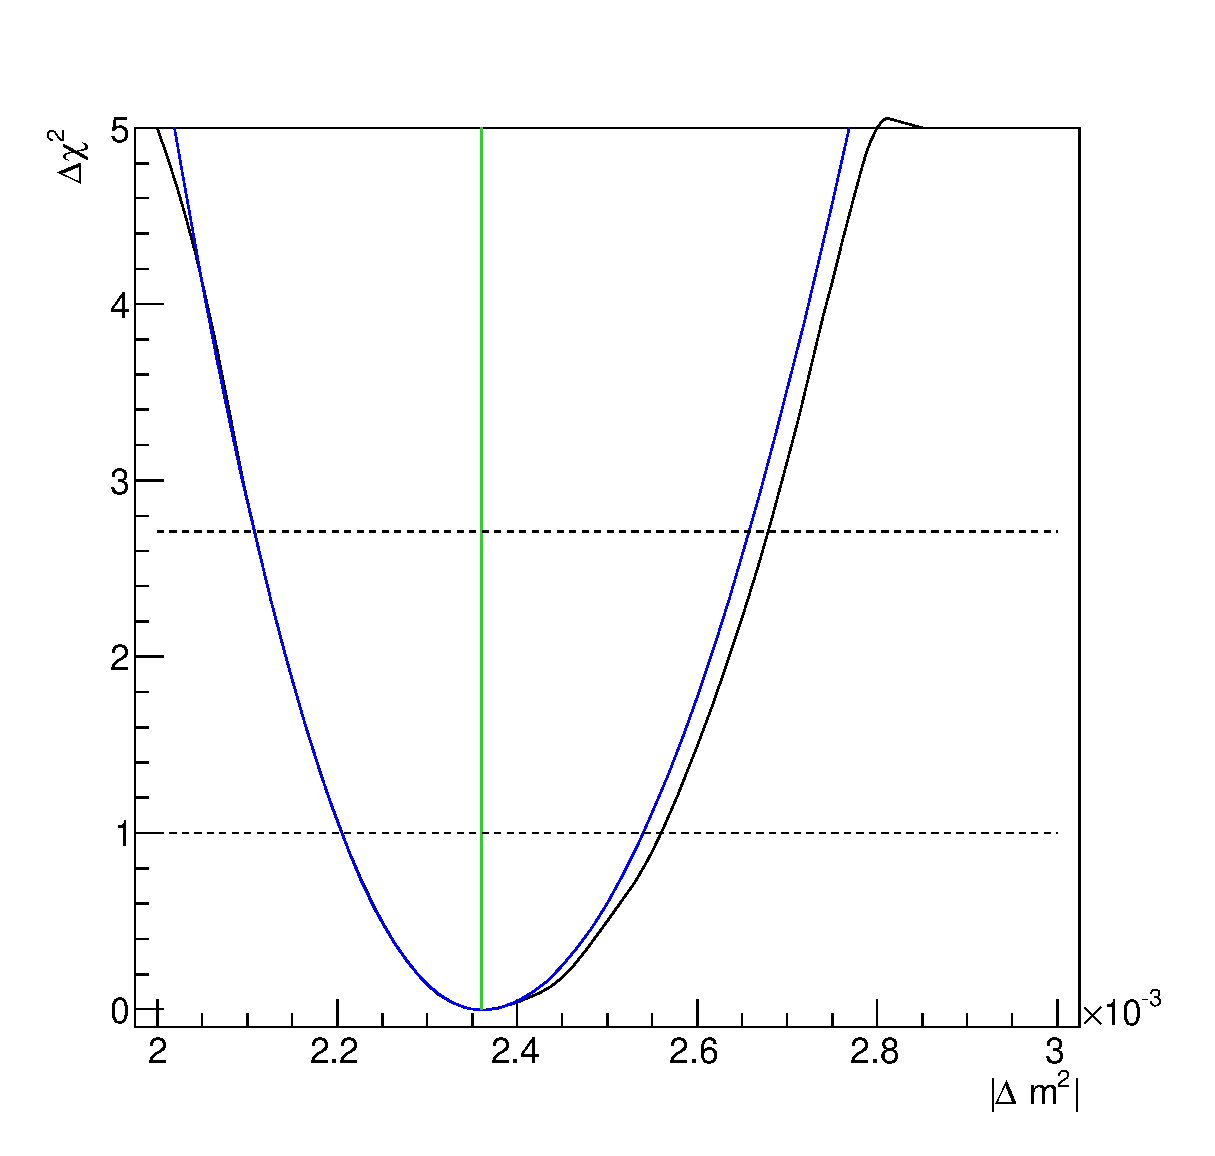
\includegraphics[width=9pc]{./images/appendix/fake_dataset_fits/fake_dataset0_chisq_dm23sq_global_min_new.eps}
\caption {
  $\Delta\chi^2$ as function of $|\Delta m^{2}|$ for fake dataset \#0.
  At each point, $\chi^2$ was minimized with respect to 
  $\sin^{2}\theta_{23}$, $\sin^{2}\theta_{13}$, $\delta_{CP}$
  and all relevant nuisance parameters for the joint analysis (black)
  and with respect to $\sin^{2}\theta_{23}$ and all relevant nuisance
  parameters for the disappearance analysis (blue).
}
\label{fig:toymc0_dchisq_Dmsq}
\end{minipage}
\hspace{0.02\linewidth}
\begin{minipage}[t]{0.22\linewidth}
\center
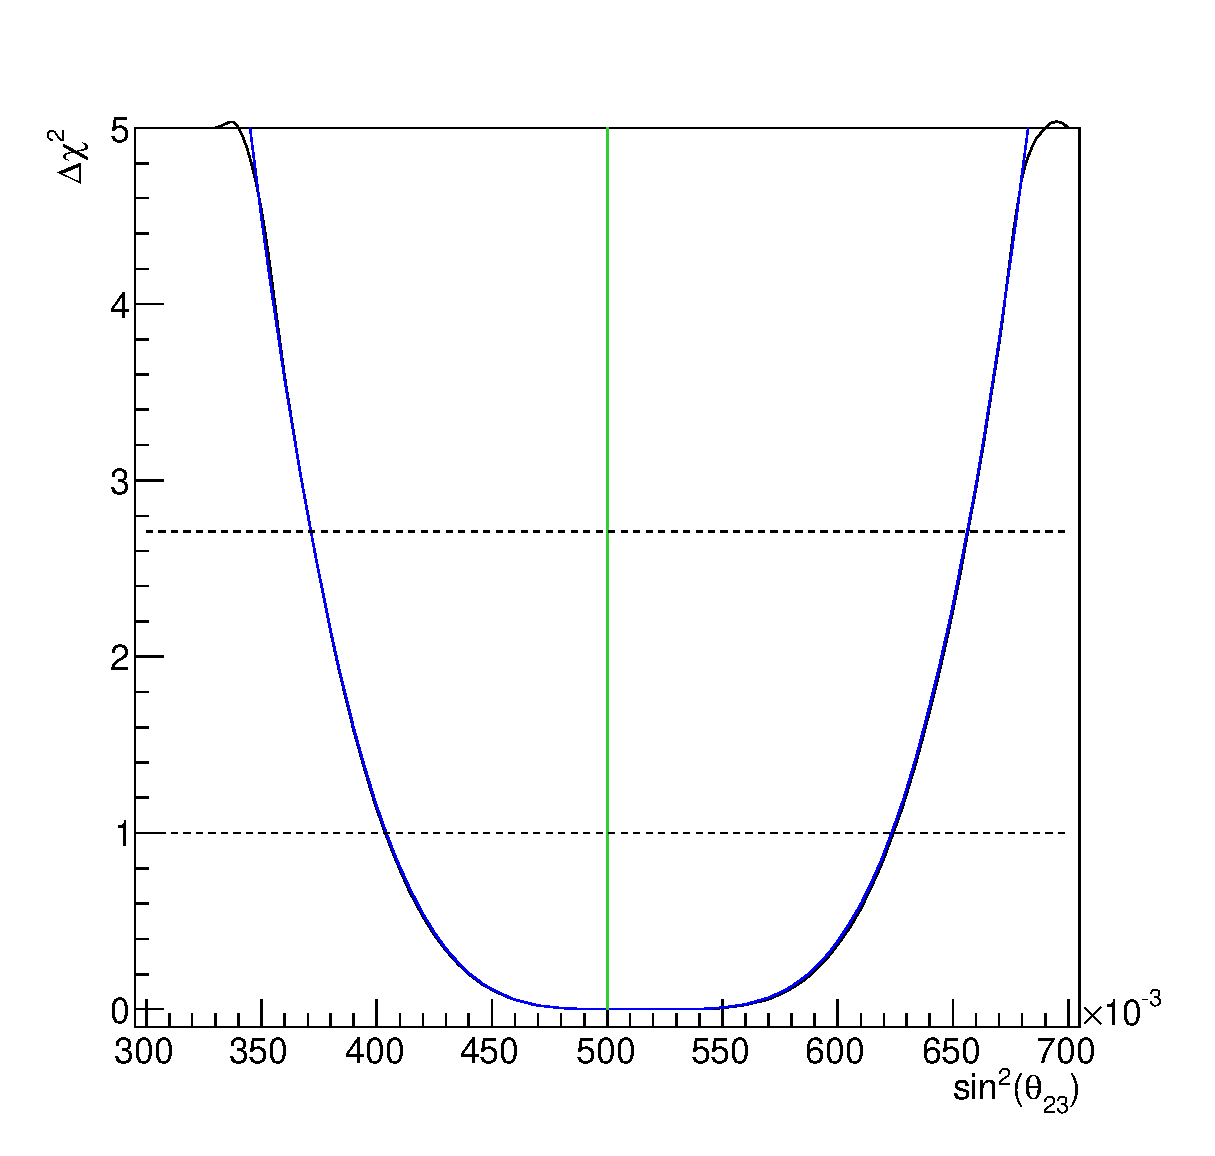
\includegraphics[width=9pc]{./images/appendix/fake_dataset_fits/fake_dataset0_chisq_theta23_global_min_new.eps}
\caption {
  $\Delta\chi^2$ as function of $sin^{2}\theta_{23}$ for fake dataset \#0.
  At each point, $\chi^2$ was minimized with respect to 
  $|\Delta m^{2}|$, $\sin^{2}\theta_{13}$, $\delta_{CP}$
  and all relevant nuisance parameters for the joint analysis (black)
  and with respect to $\sin^{2}\theta_{23}$ and all relevant nuisance
  parameters for the disappearance analysis (blue).
}
\label{fig:toymc0_dchisq_sinsqtheta23}
\end{minipage}
\hspace{0.02\linewidth}
\begin{minipage}[t]{0.22\linewidth}
\center
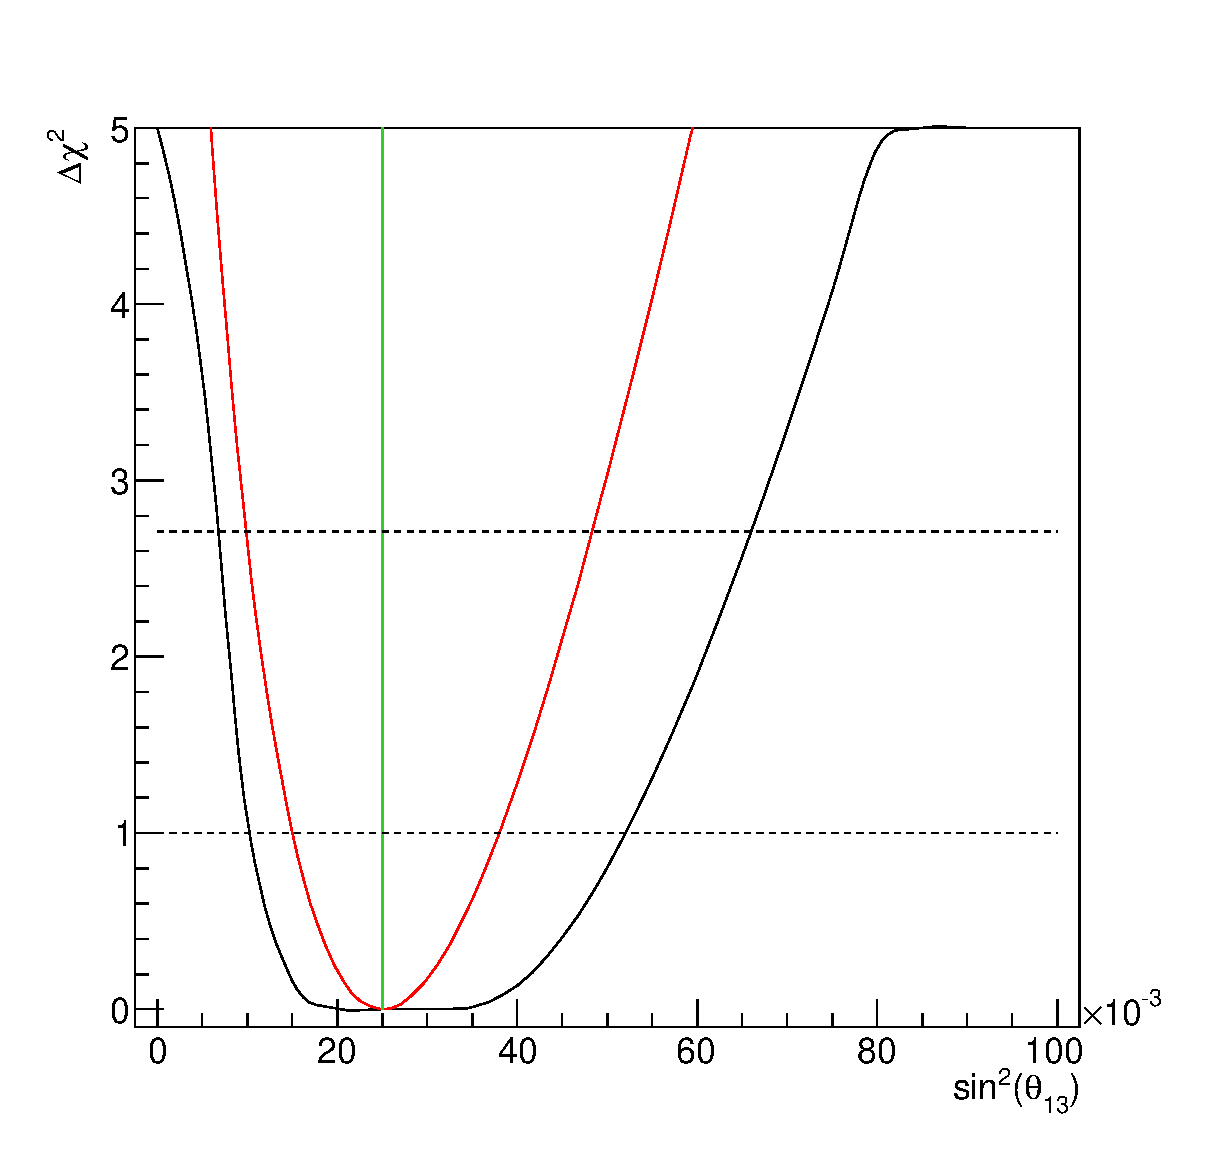
\includegraphics[width=9pc]{./images/appendix/fake_dataset_fits/fake_dataset0_chisq_theta13_global_min_new.eps}
\caption {
  $\Delta\chi^2$ as function of $sin^{2}\theta_{13}$ for fake dataset \#0.
  At each point, $\chi^2$ was minimized with respect to 
  $\sin^{2}\theta_{23}$, $\sin^{2}\theta_{13}$, $\delta_{CP}$
  and all relevant nuisance parameters for the joint analysis (black)
  and with respect to all relevant nuisance parameters 
  ($\delta_{CP}$ is fixed to 0) for the appearance analysis (red).
}
\label{fig:toymc0_dchisq_sinsqtheta13}
\end{minipage}
\hspace{0.02\linewidth}
\begin{minipage}[t]{0.22\linewidth}
\center
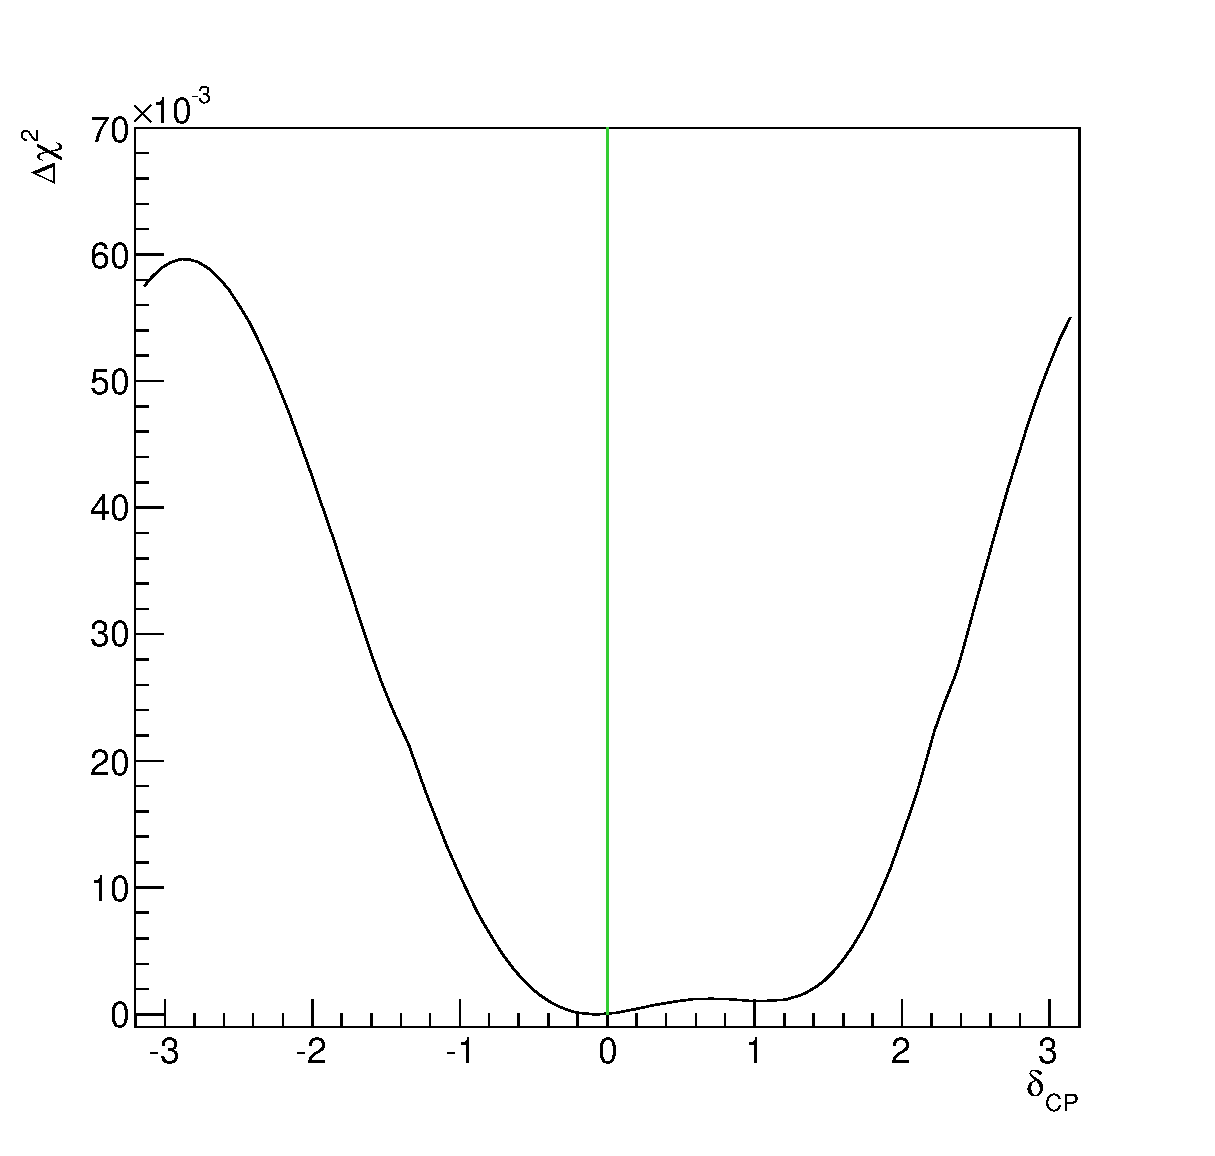
\includegraphics[width=9pc]{.//images/appendix/fake_dataset_fits/fake_dataset0_chisq_deltacp_global_min_new.eps}
\caption {
  $\Delta\chi^2$ as function of $\delta_{CP}$ for fake dataset \#0.
  At each point, $\chi^2$ was minimized with respect to 
  all oscillation parameters not shown (and not considered to be fixed)
  and all relevant nuisance parameters.
}
\label{fig:toymc0_dchisq_deltacp}
\end{minipage}

\vfill
\vspace*{0.7cm}

\begin{minipage}[t]{0.48\linewidth}
\center
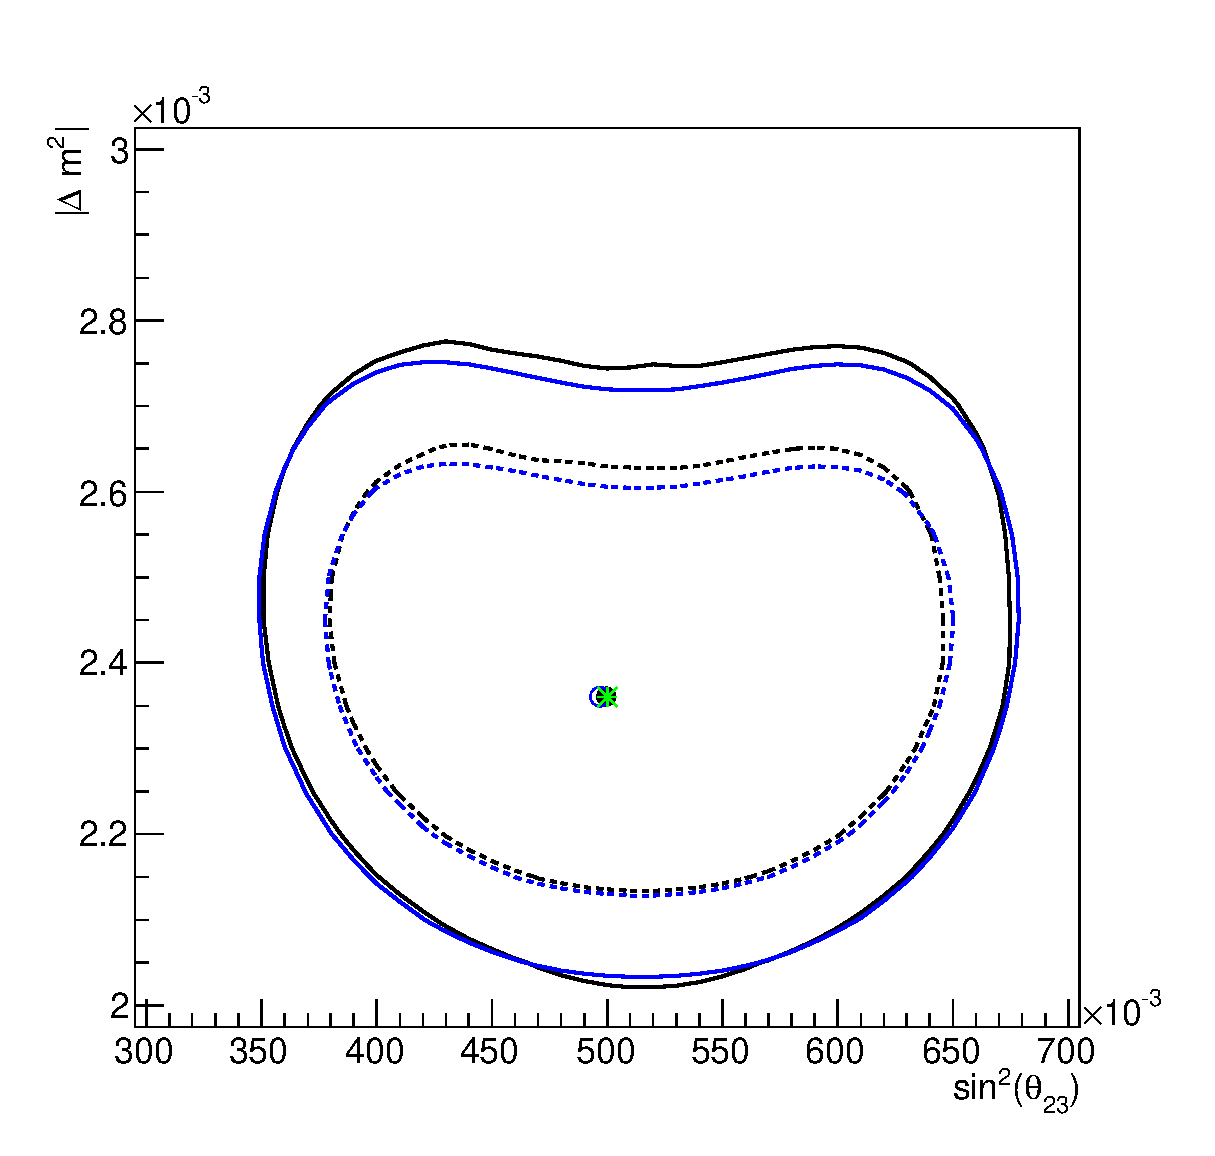
\includegraphics[width=15pc]{./images/appendix/fake_dataset_fits/fake_dataset0_chisq_theta23_dm23sq_global_min_new.eps}
\caption {
  68\% and 90\% CL regions in ($sin^{2}\theta_{23}$, $|\Delta m^{2}|$) space for fake dataset \#0.
  At each point, $\chi^2$ was minimized with respect to 
  $\sin^{2}\theta_{13}$, $\delta_{CP}$
  and all relevant nuisance parameters for the joint analysis (black)
  and with respect to all relevant nuisance parameters for the disappearance analysis (blue). 
}
\label{fig:toymc0_confreg_sinsqtheta23_Dmsq}
\end{minipage}
\hspace{0.03\linewidth}
\begin{minipage}[t]{0.48\linewidth}
\center
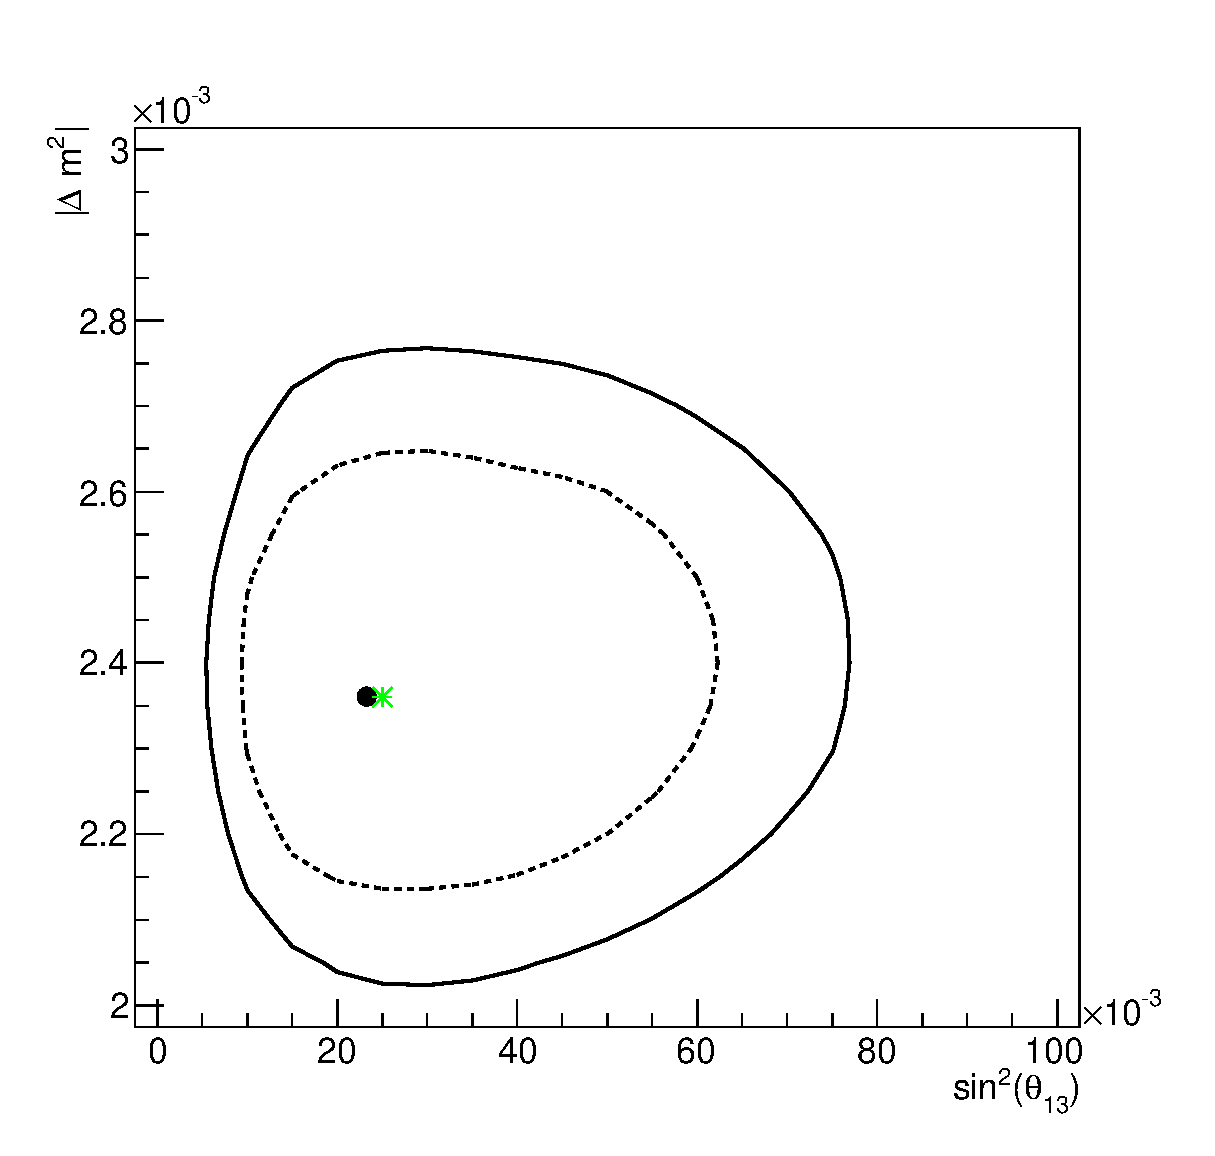
\includegraphics[width=15pc]{./images/appendix/fake_dataset_fits/fake_dataset0_chisq_theta13_dm23sq_global_min_new.eps}
\caption {
  68\% and 90\% CL regions in ($sin^{2}\theta_{13}$, $|\Delta m^{2}|$) space for fake dataset \#0.
  At each point, $\chi^2$ was minimized with respect to 
  all oscillation parameters not shown (and not considered to be fixed)
  and all relevant nuisance parameters.
}
\label{fig:toymc0_confreg_sinsqtheta13_Dmsq}
\end{minipage}

\vfill
\vspace*{0.7cm}

\begin{minipage}[t]{0.48\linewidth}
\center
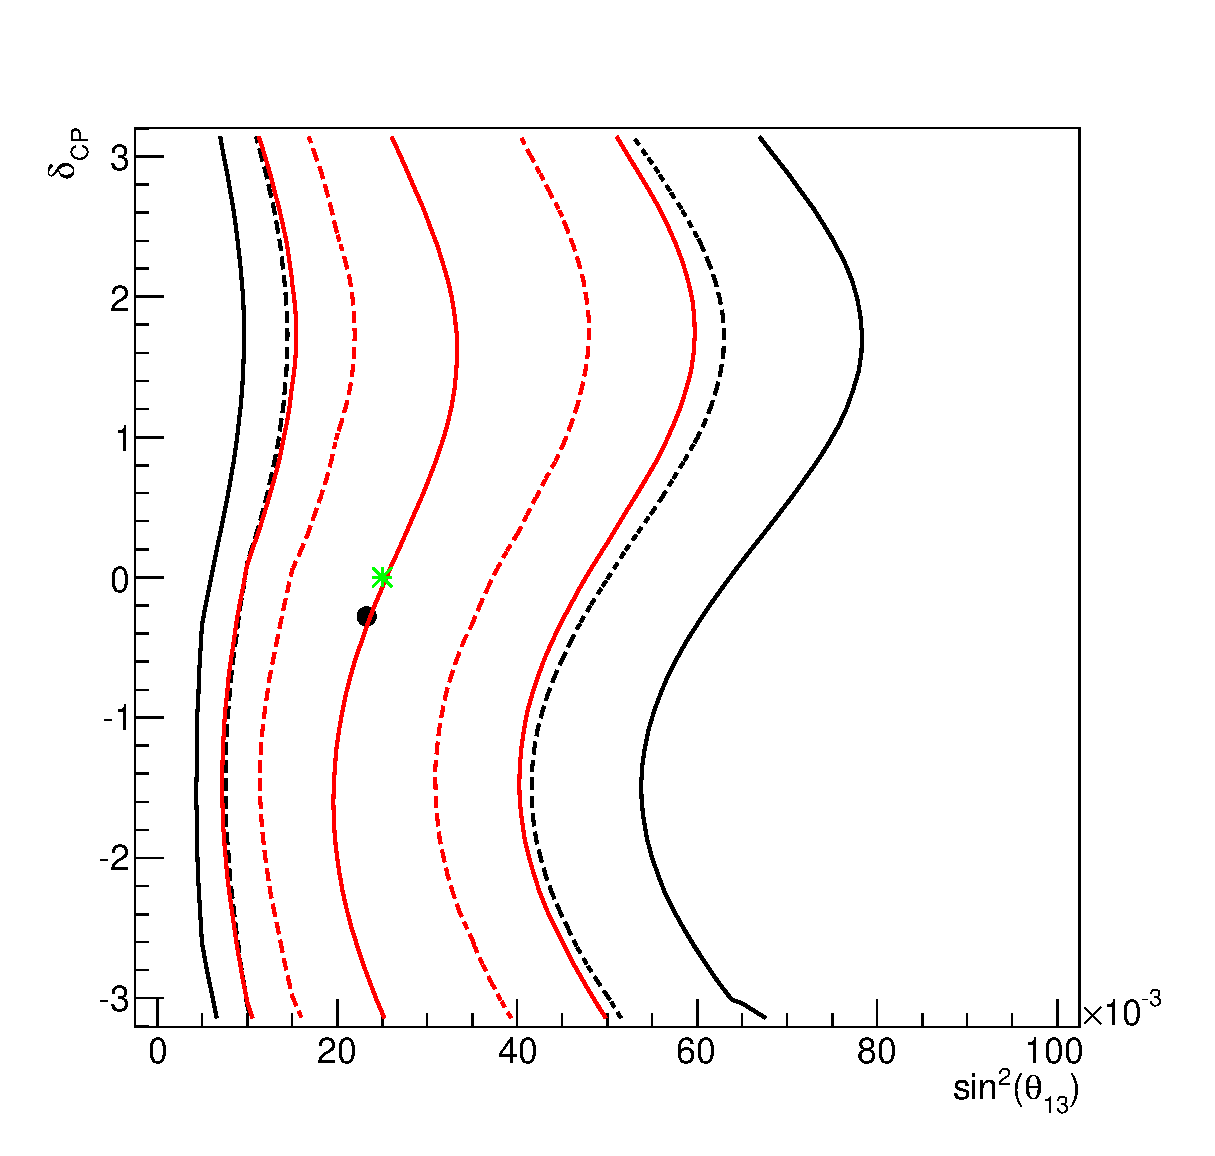
\includegraphics[width=15pc]{./images/appendix/fake_dataset_fits/fake_dataset0_chisq_theta13_deltacp_global_min_new.eps}
\caption {
  68\% and 90\% CL regions in ($sin^{2}\theta_{13}$, $\delta_{CP}$) space for fake dataset \#0.
  At each point, $\chi^2$ was minimized with respect to 
  $|\Delta m^{2}|$, $\sin^{2}\theta_{23}$
  and all relevant nuisance parameters for the joint analysis (black)
  and with respect to all relevant nuisance parameters for the appearance analysis (red).
  Notice that different methods are used to
  construct confidence regions for the joint analysis (global minimum) and for the 
  stand-alone appearance analysis (raster scan).
}
\label{fig:toymc0_confreg_sinsqtheta13_deltacp}
\end{minipage}
\hspace{0.03\linewidth}
\begin{minipage}[t]{0.48\linewidth}
\center
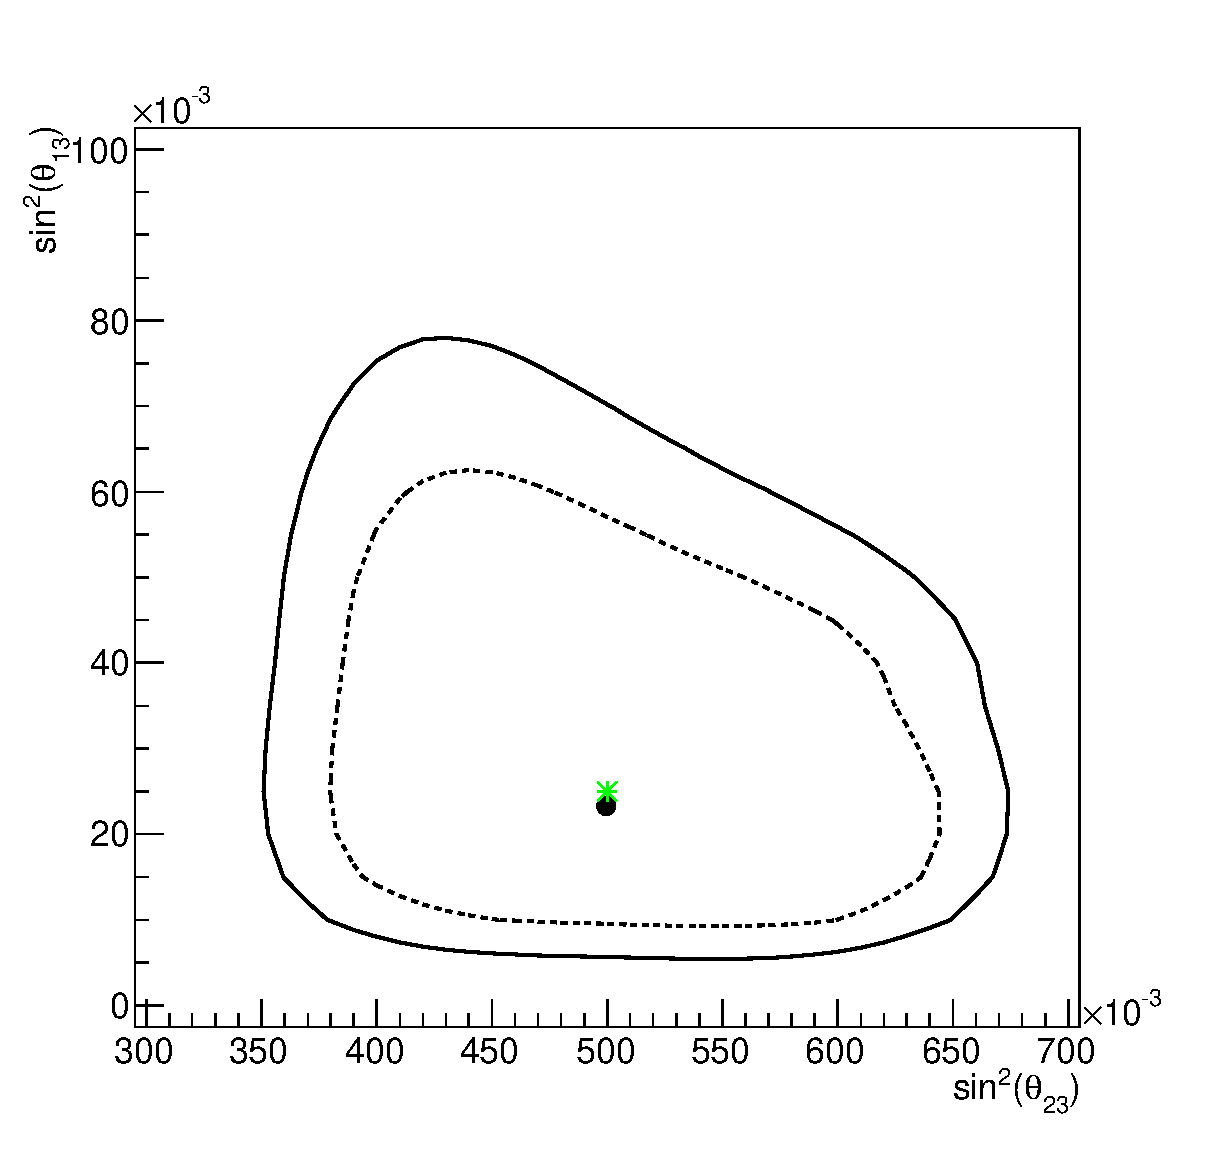
\includegraphics[width=15pc]{./images/appendix/fake_dataset_fits/fake_dataset0_chisq_theta13_theta23_global_min_new.eps}
\caption {
  68\% and 90\% CL regions in ($sin^{2}\theta_{23}$, $sin^{2}\theta_{13}$) space for fake dataset \#0.
  At each point, $\chi^2$ was minimized with respect to 
  all oscillation parameters not shown (and not considered to be fixed)
  and all relevant nuisance parameters.
}
\label{fig:toymc0_confreg_sinsqtheta23_sinsqtheta13}
\end{minipage}

\end{figure*}

\clearpage

%
%
% ..............................................
% Fake dataset #1
%
%


%
% delta\chisq and contours
%

\begin{figure*}[htb]

\begin{minipage}[t]{0.22\linewidth}
\center
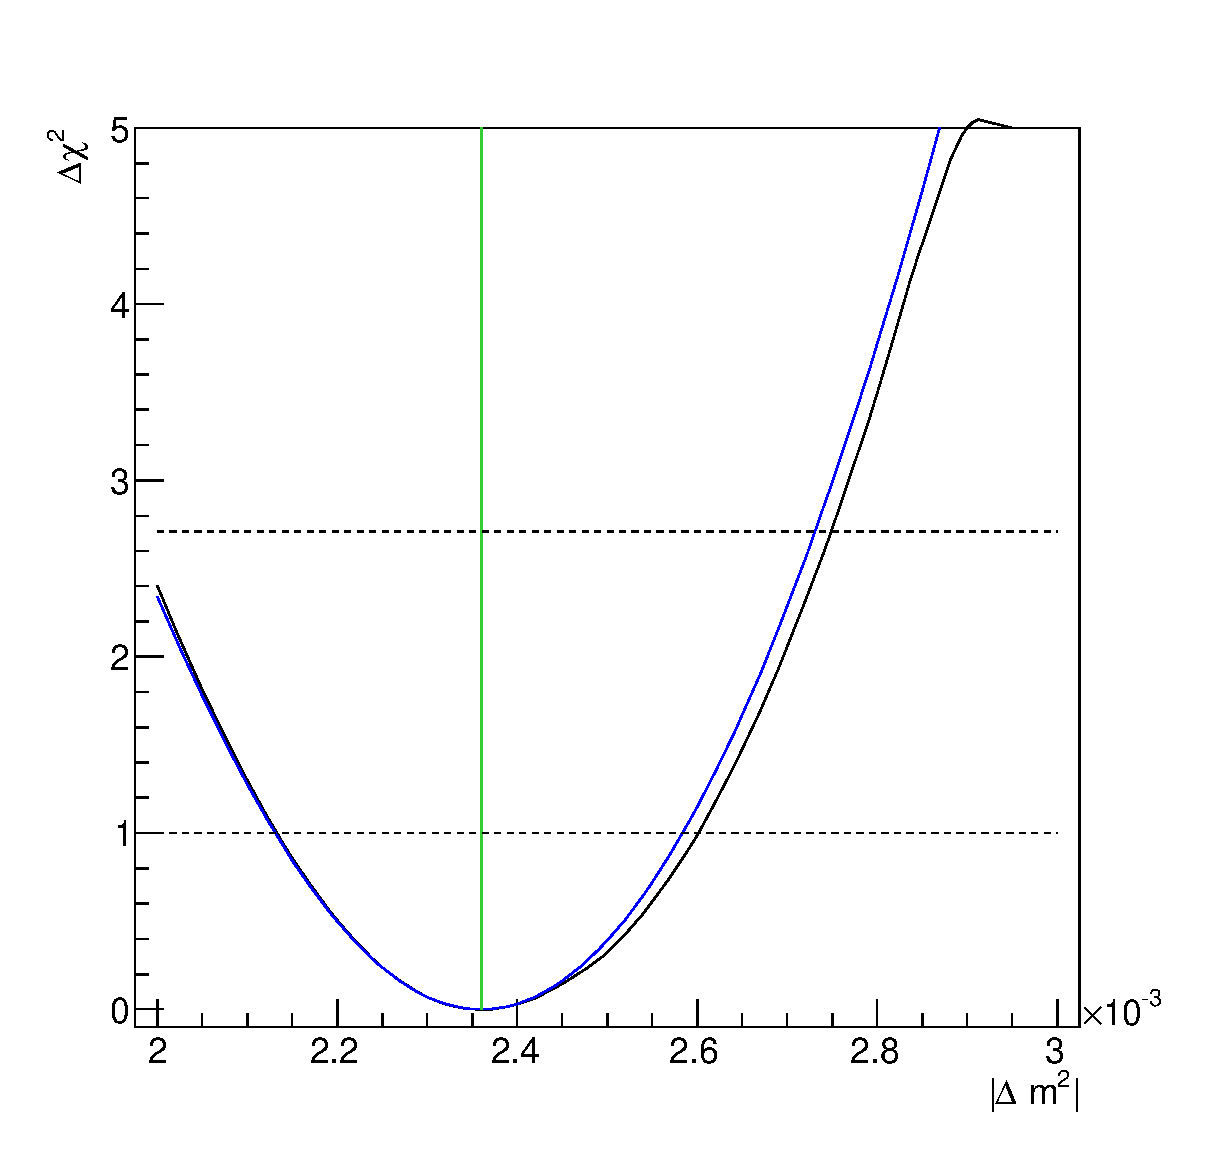
\includegraphics[width=9pc]{./images/appendix/fake_dataset_fits/fake_dataset1_chisq_dm23sq_global_min_new.eps}
\caption {
  $\Delta\chi^2$ as function of $|\Delta m^{2}|$ for fake dataset \#1.
  At each point, $\chi^2$ was minimized with respect to 
  $\sin^{2}\theta_{23}$, $\sin^{2}\theta_{13}$, $\delta_{CP}$
  and all relevant nuisance parameters for the joint analysis (black)
  and with respect to $\sin^{2}\theta_{23}$ and all relevant nuisance
  parameters for the disappearance analysis (blue).
}
\label{fig:toymc1_dchisq_Dmsq}
\end{minipage}
\hspace{0.02\linewidth}
\begin{minipage}[t]{0.22\linewidth}
\center
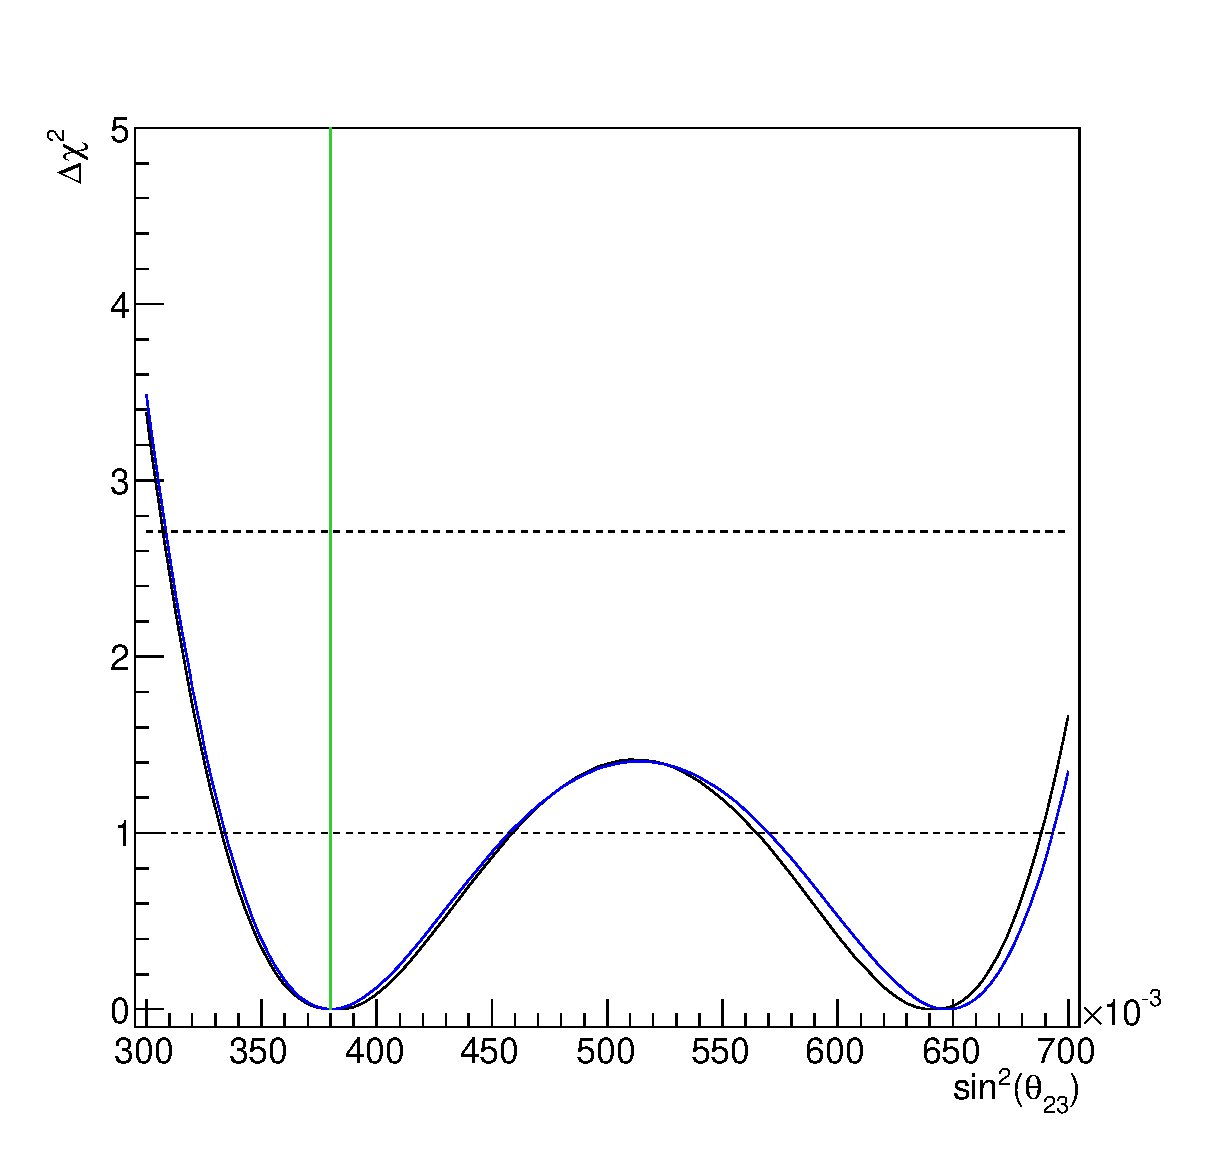
\includegraphics[width=9pc]{./images/appendix/fake_dataset_fits/fake_dataset1_chisq_theta23_global_min_new.eps}
\caption {
  $\Delta\chi^2$ as function of $sin^{2}\theta_{23}$ for fake dataset \#1.
  At each point, $\chi^2$ was minimized with respect to 
  $|\Delta m^{2}|$, $\sin^{2}\theta_{13}$, $\delta_{CP}$
  and all relevant nuisance parameters for the joint analysis (black)
  and with respect to $\sin^{2}\theta_{23}$ and all relevant nuisance
  parameters for the disappearance analysis (blue).
}
\label{fig:toymc1_dchisq_sinsqtheta23}
\end{minipage}
\hspace{0.02\linewidth}
\begin{minipage}[t]{0.22\linewidth}
\center
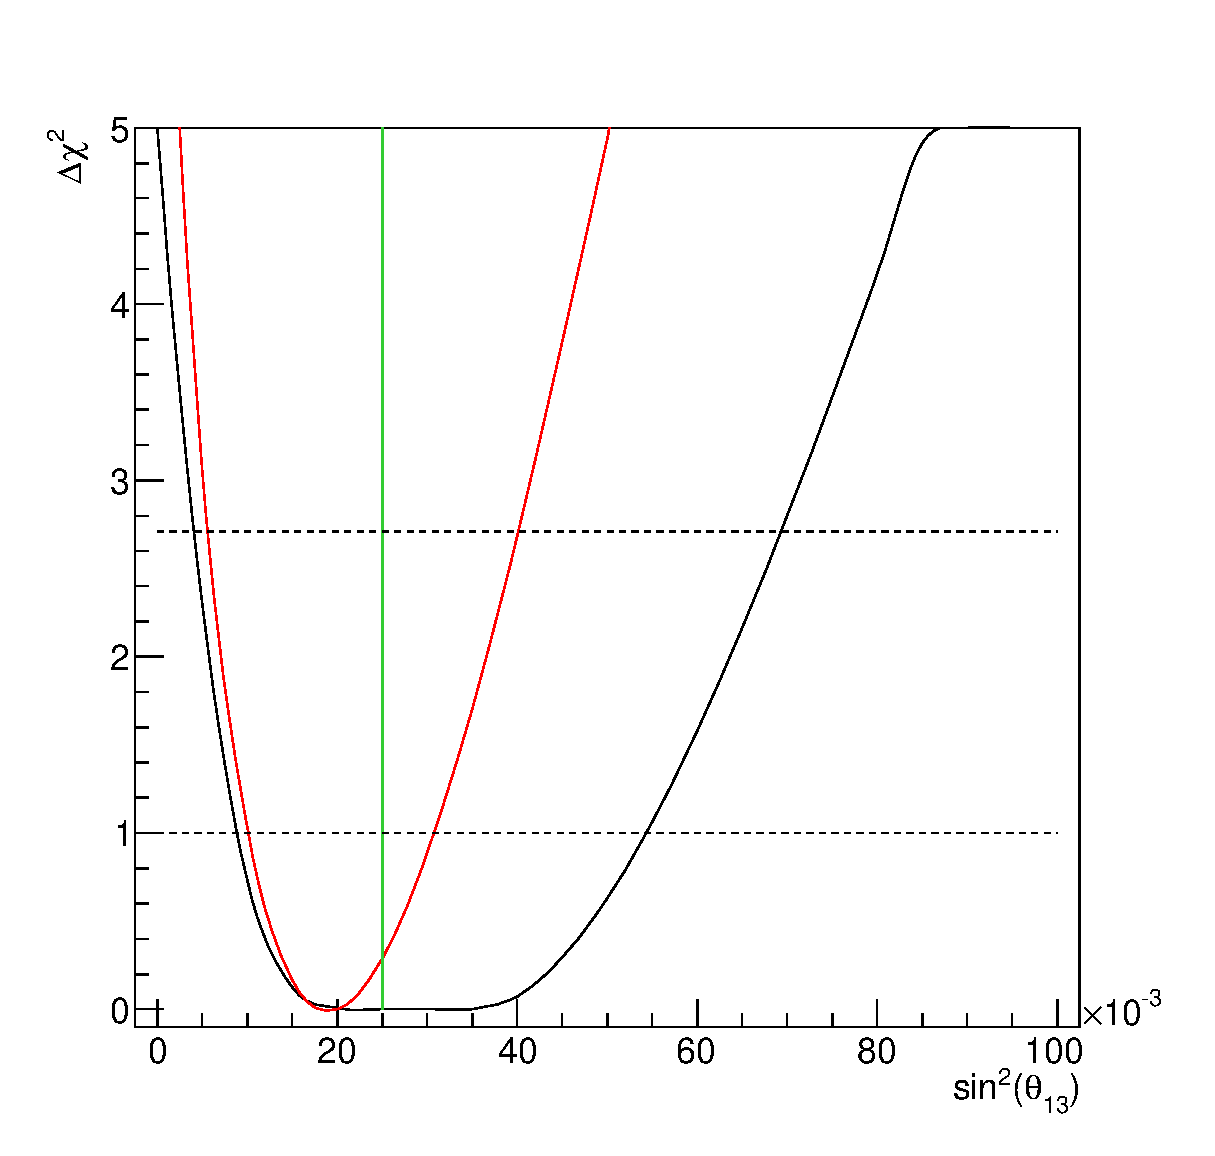
\includegraphics[width=9pc]{./images/appendix/fake_dataset_fits/fake_dataset1_chisq_theta13_global_min_new.eps}
\caption {
  $\Delta\chi^2$ as function of $sin^{2}\theta_{13}$ for fake dataset \#1.
  At each point, $\chi^2$ was minimized with respect to 
  $\sin^{2}\theta_{23}$, $\sin^{2}\theta_{13}$, $\delta_{CP}$
  and all relevant nuisance parameters for the joint analysis (black)
  and with respect to all relevant nuisance parameters 
  ($\delta_{CP}$ is fixed to 0) for the appearance analysis (red).
}
\label{fig:toymc1_dchisq_sinsqtheta13}
\end{minipage}
\hspace{0.02\linewidth}
\begin{minipage}[t]{0.22\linewidth}
\center
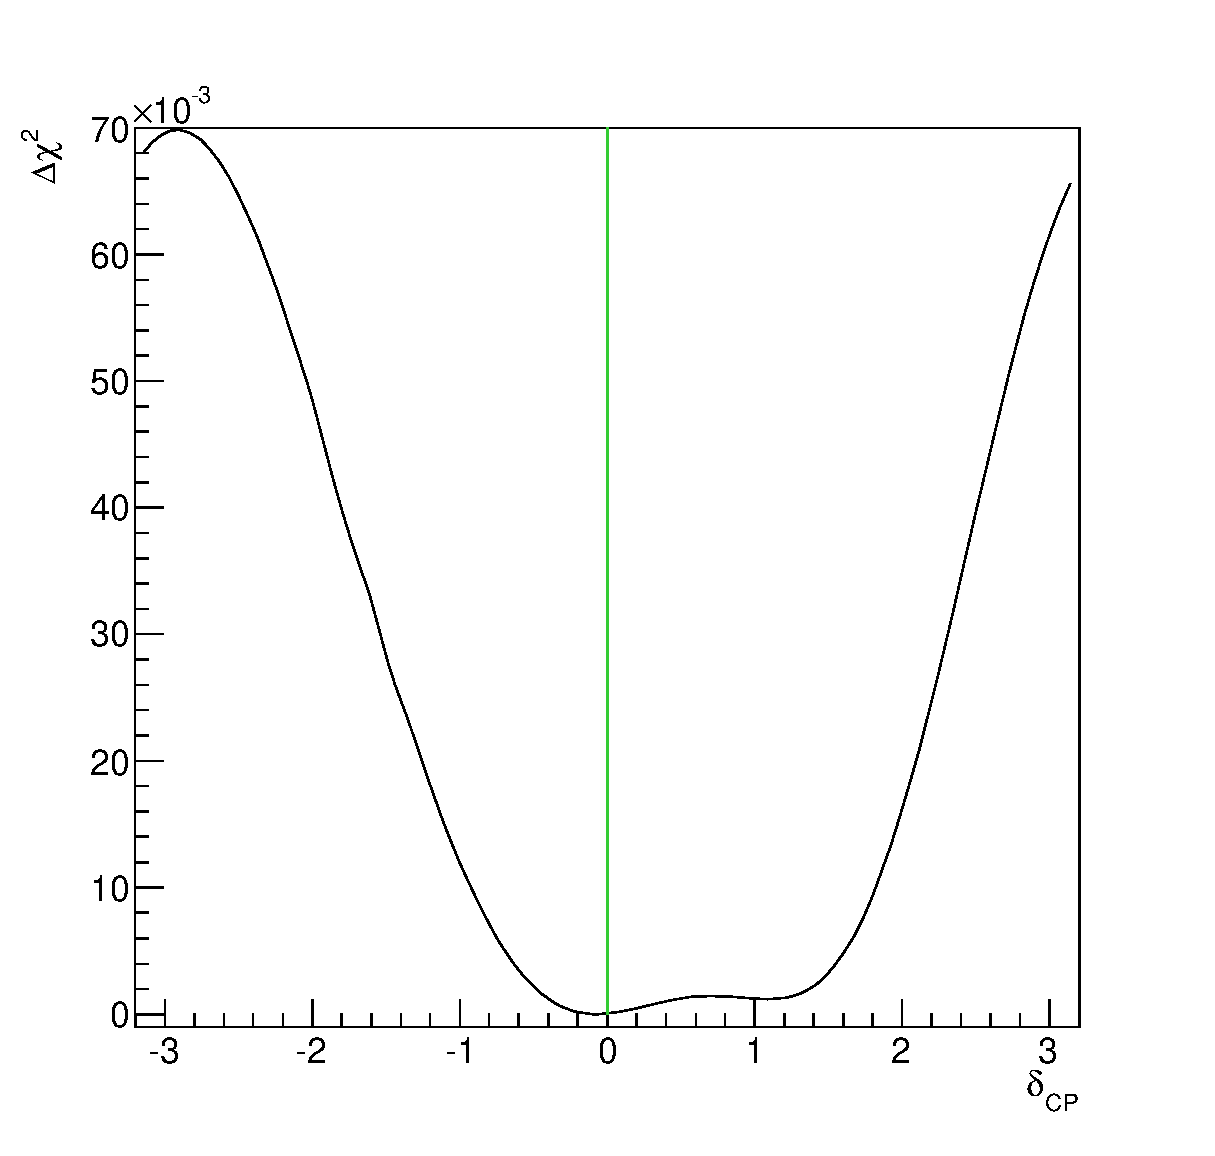
\includegraphics[width=9pc]{.//images/appendix/fake_dataset_fits/fake_dataset1_chisq_deltacp_global_min_new.eps}
\caption {
  $\Delta\chi^2$ as function of $\delta_{CP}$ for fake dataset \#1.
  At each point, $\chi^2$ was minimized with respect to 
  all oscillation parameters not shown (and not considered to be fixed)
  and all relevant nuisance parameters.
}
\label{fig:toymc1_dchisq_deltacp}
\end{minipage}

\vfill
\vspace*{0.7cm}

\begin{minipage}[t]{0.48\linewidth}
\center
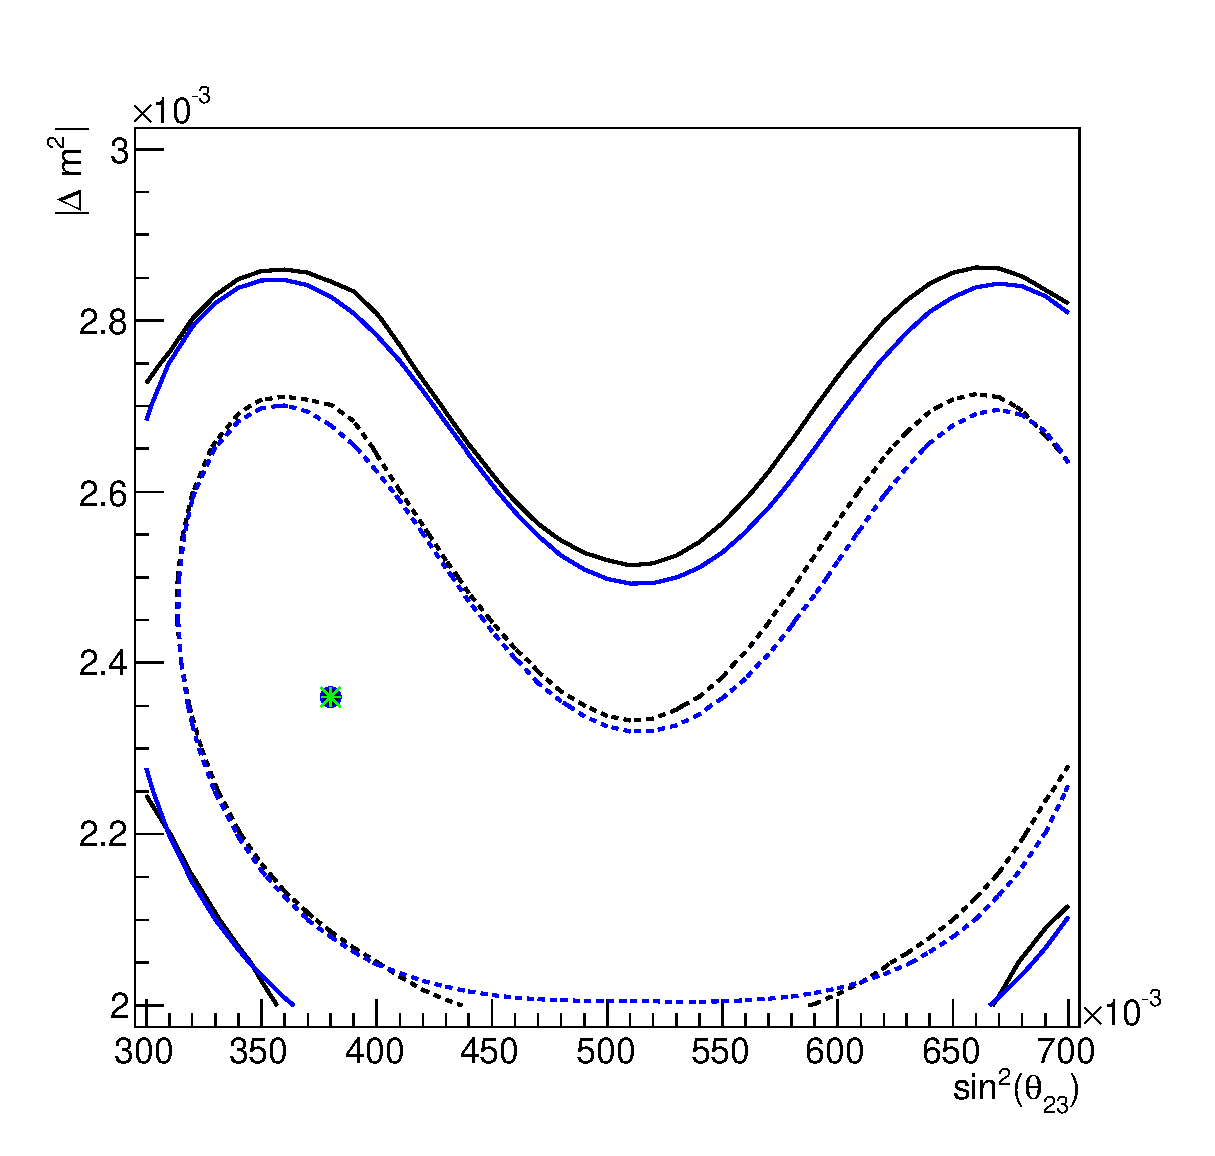
\includegraphics[width=15pc]{./images/appendix/fake_dataset_fits/fake_dataset1_chisq_theta23_dm23sq_global_min_new.eps}
\caption {
  68\% and 90\% CL regions in ($sin^{2}\theta_{23}$, $|\Delta m^{2}|$) space for fake dataset \#1.
  At each point, $\chi^2$ was minimized with respect to 
  $\sin^{2}\theta_{13}$, $\delta_{CP}$
  and all relevant nuisance parameters for the joint analysis (black)
  and with respect to all relevant nuisance parameters for the disappearance analysis (blue).
  }
\label{fig:toymc1_confreg_sinsqtheta23_Dmsq}
\end{minipage}
\hspace{0.03\linewidth}
\begin{minipage}[t]{0.48\linewidth}
\center
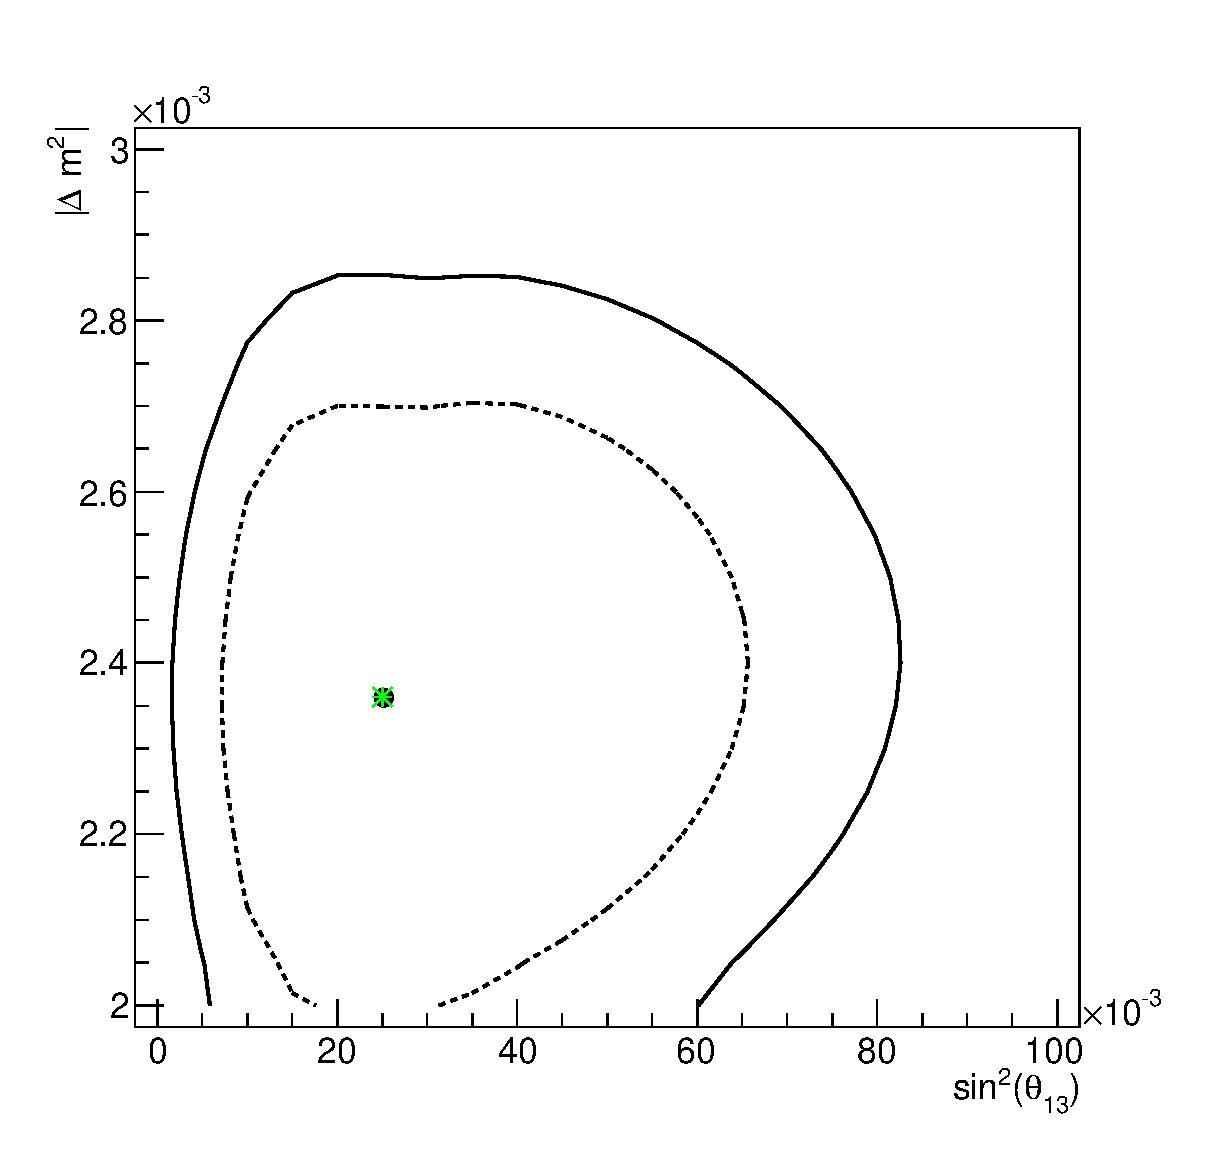
\includegraphics[width=15pc]{./images/appendix/fake_dataset_fits/fake_dataset1_chisq_theta13_dm23sq_global_min_new.eps}
\caption {
  68\% and 90\% CL regions in ($sin^{2}\theta_{13}$, $|\Delta m^{2}|$) space for fake dataset \#1.
  At each point, $\chi^2$ was minimized with respect to 
  all oscillation parameters not shown (and not considered to be fixed)
  and all relevant nuisance parameters.
}
\label{fig:toymc1_confreg_sinsqtheta13_Dmsq}
\end{minipage}

\vfill
\vspace*{0.7cm}

\begin{minipage}[t]{0.48\linewidth}
\center
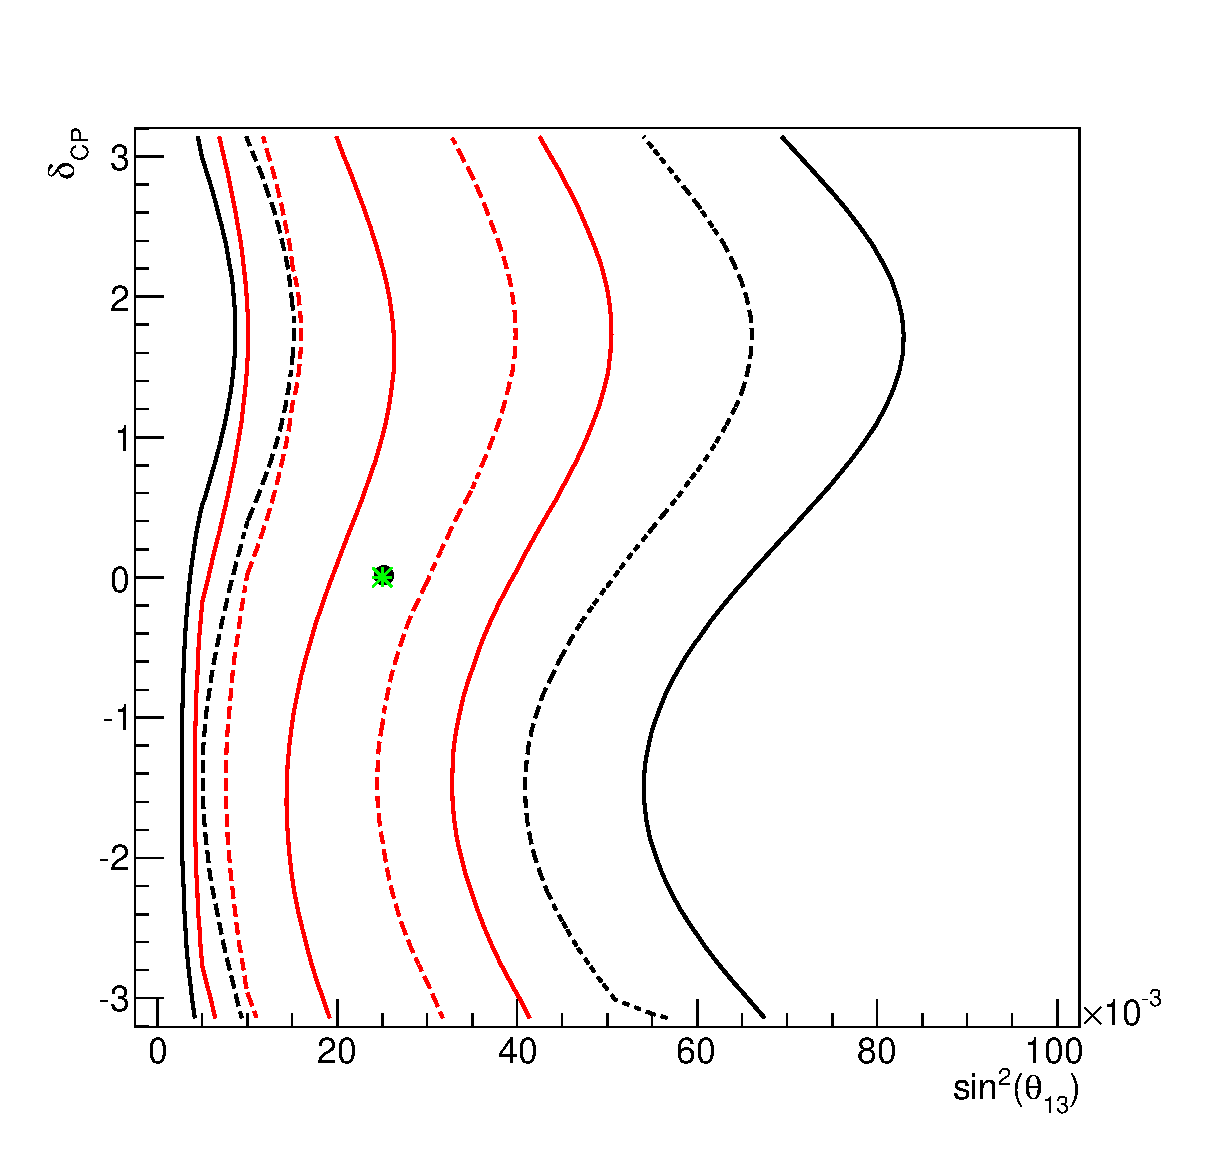
\includegraphics[width=15pc]{./images/appendix/fake_dataset_fits/fake_dataset1_chisq_theta13_deltacp_global_min_new.eps}
\caption {
  68\% and 90\% CL regions in ($sin^{2}\theta_{13}$, $\delta_{CP}$) space for fake dataset \#1.
  At each point, $\chi^2$ was minimized with respect to 
  $|\Delta m^{2}|$, $\sin^{2}\theta_{23}$
  and all relevant nuisance parameters for the joint analysis (black)
  and with respect to all relevant nuisance parameters for the appearance analysis (red).
  Notice that different methods are used to
  construct confidence regions for the joint analysis (global minimum) and for the 
  stand-alone appearance analysis (raster scan).
}
\label{fig:toymc1_confreg_sinsqtheta13_deltacp}
\end{minipage}
\hspace{0.03\linewidth}
\begin{minipage}[t]{0.48\linewidth}
\center
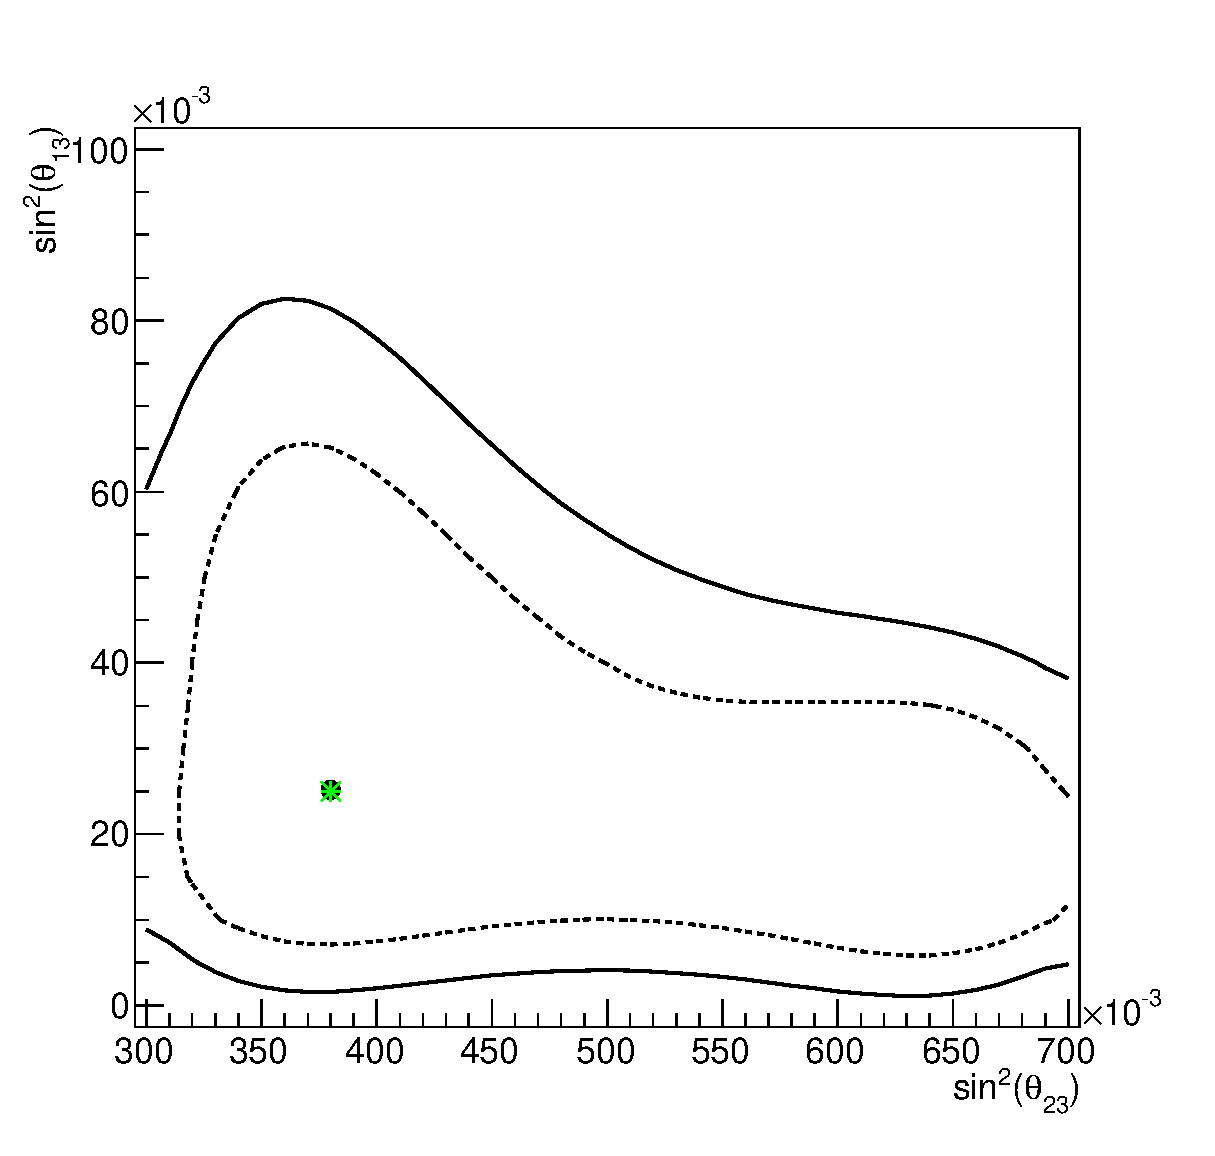
\includegraphics[width=15pc]{./images/appendix/fake_dataset_fits/fake_dataset1_chisq_theta13_theta23_global_min_new.eps}
\caption {
  68\% and 90\% CL regions in ($sin^{2}\theta_{23}$, $sin^{2}\theta_{13}$) space for fake dataset \#1.
  At each point, $\chi^2$ was minimized with respect to 
  all oscillation parameters not shown (and not considered to be fixed)
  and all relevant nuisance parameters.
}
\label{fig:toymc1_confreg_sinsqtheta23_sinsqtheta13}
\end{minipage}

\end{figure*}

%
%
% ..............................................
% Fake dataset #2
%
%

\clearpage

%
% delta\chisq and contours
%

\begin{figure*}[htb]

\begin{minipage}[t]{0.22\linewidth}
\center
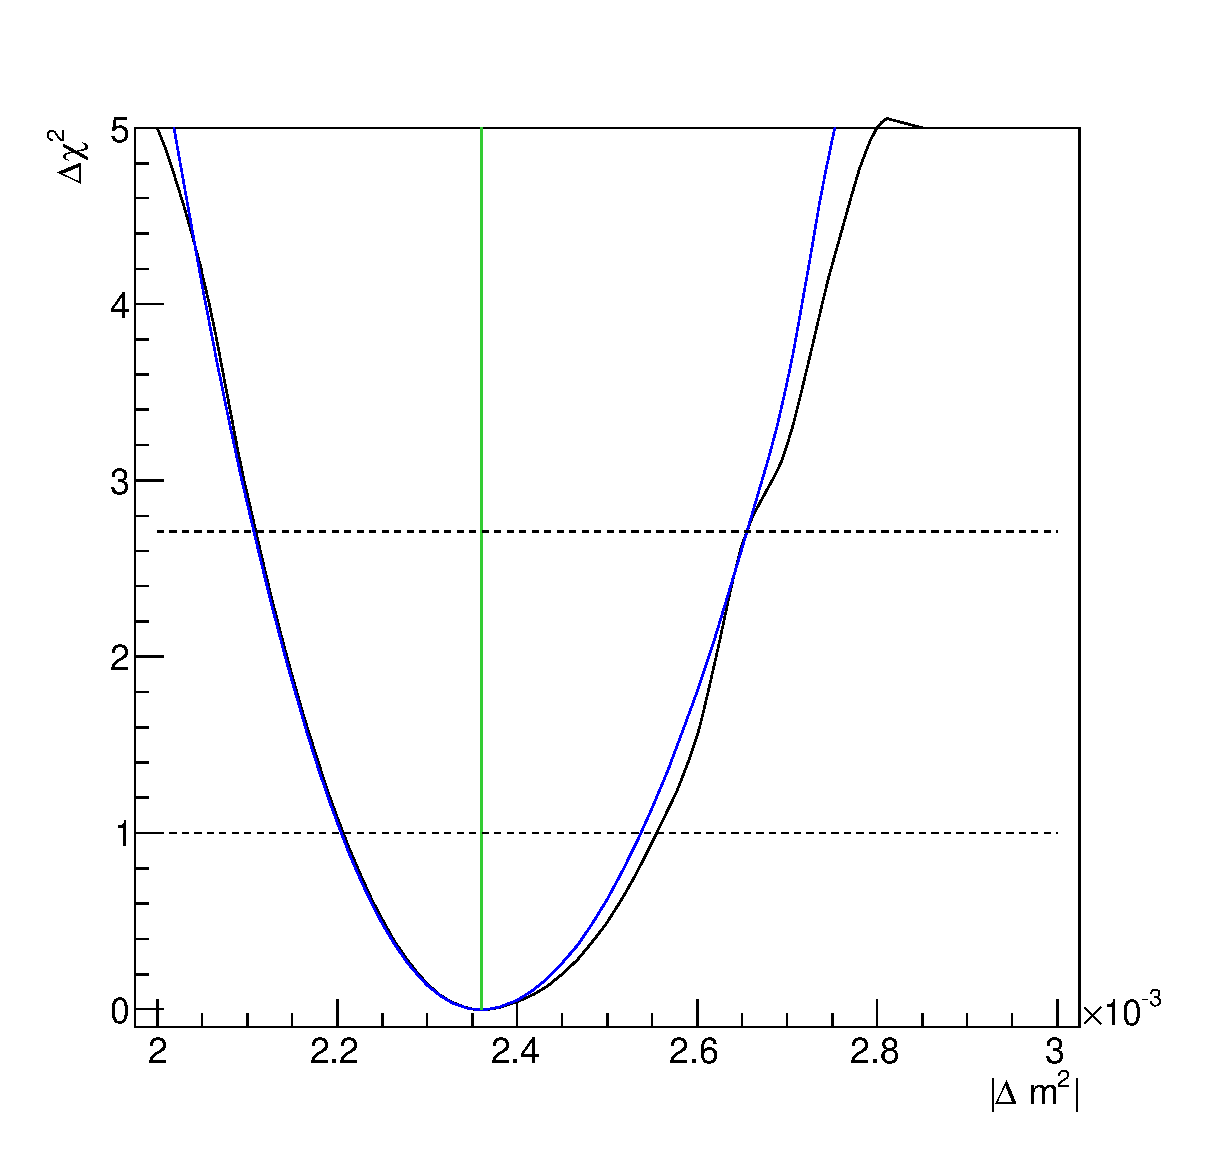
\includegraphics[width=9pc]{./images/appendix/fake_dataset_fits/fake_dataset3_chisq_dm23sq_global_min_new.eps}
\caption {
  $\Delta\chi^2$ as function of $|\Delta m^{2}|$ for fake dataset \#2.
  At each point, $\chi^2$ was minimized with respect to 
  $\sin^{2}\theta_{23}$, $\sin^{2}\theta_{13}$, $\delta_{CP}$
  and all relevant nuisance parameters for the joint analysis (black)
  and with respect to $\sin^{2}\theta_{23}$ and all relevant nuisance
  parameters for the disappearance analysis (blue).
}
\label{fig:toymc2_dchisq_Dmsq}
\end{minipage}
\hspace{0.02\linewidth}
\begin{minipage}[t]{0.22\linewidth}
\center
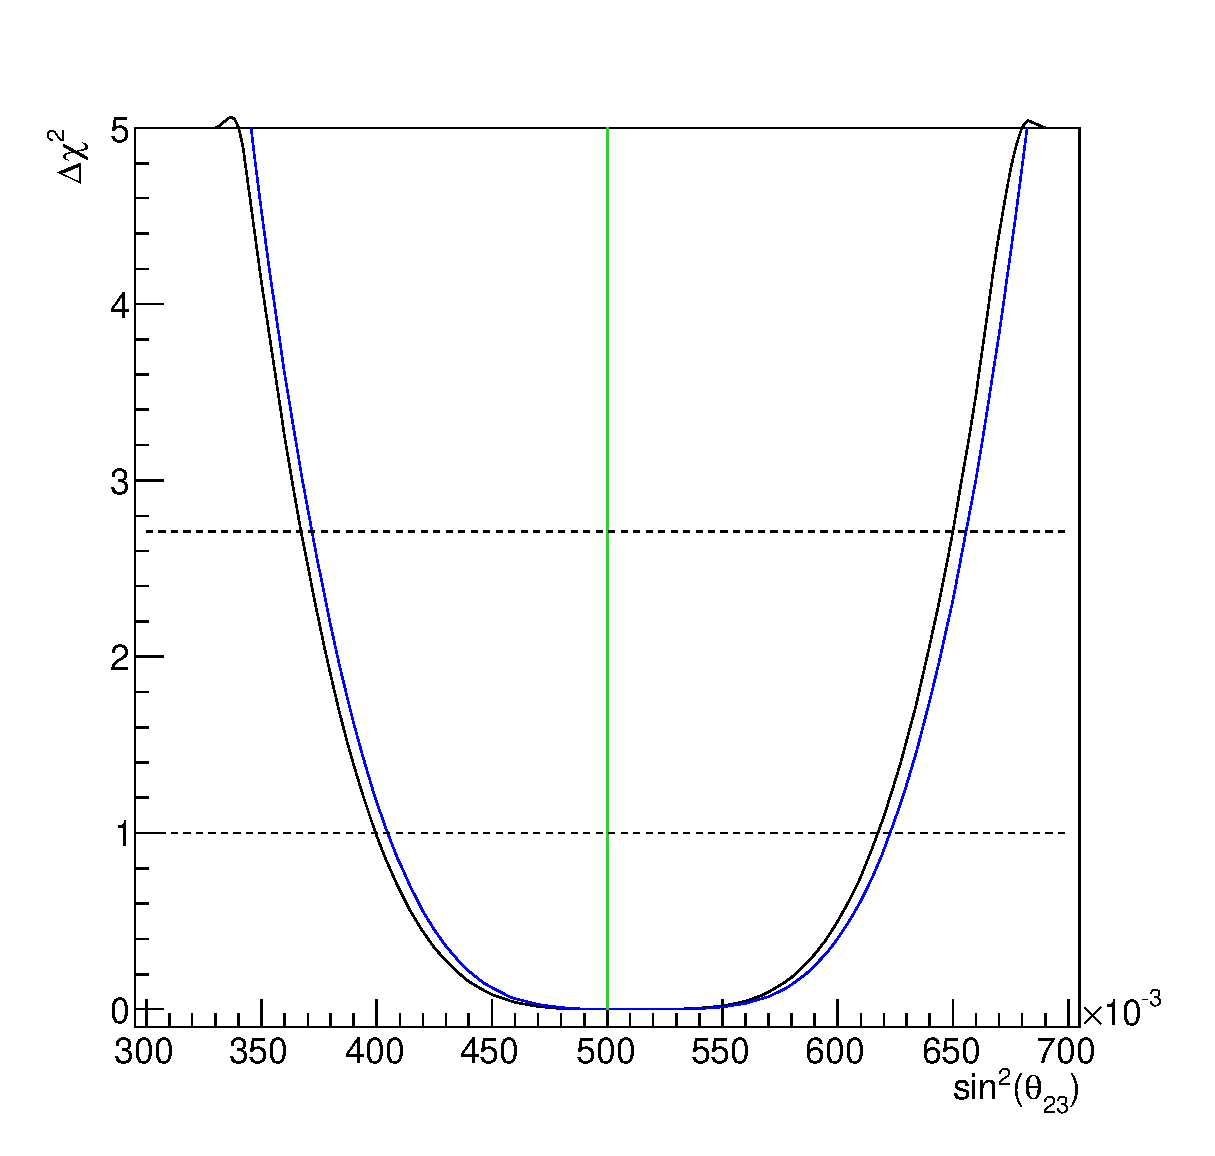
\includegraphics[width=9pc]{./images/appendix/fake_dataset_fits/fake_dataset3_chisq_theta23_global_min_new.eps}
\caption {
  $\Delta\chi^2$ as function of $sin^{2}\theta_{23}$ for fake dataset \#2.
  At each point, $\chi^2$ was minimized with respect to 
  $|\Delta m^{2}|$, $\sin^{2}\theta_{13}$, $\delta_{CP}$
  and all relevant nuisance parameters for the joint analysis (black)
  and with respect to $\sin^{2}\theta_{23}$ and all relevant nuisance
  parameters for the disappearance analysis (blue).
}
\label{fig:toymc2_dchisq_sinsqtheta23}
\end{minipage}
\hspace{0.02\linewidth}
\begin{minipage}[t]{0.22\linewidth}
\center
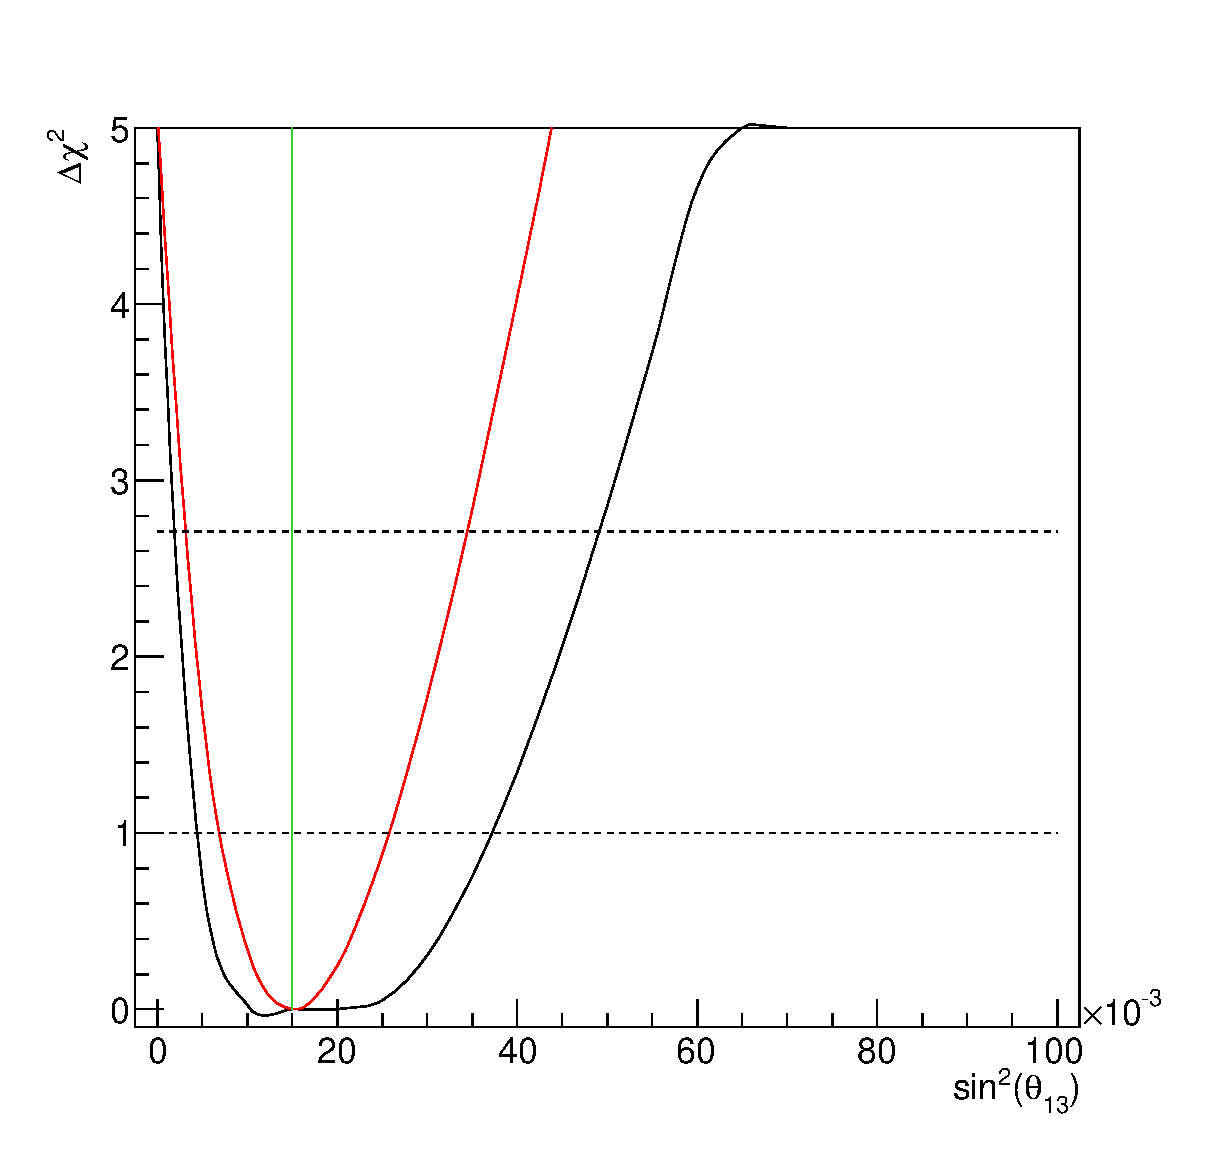
\includegraphics[width=9pc]{./images/appendix/fake_dataset_fits/fake_dataset3_chisq_theta13_global_min_new.eps}
\caption {
  $\Delta\chi^2$ as function of $sin^{2}\theta_{13}$ for fake dataset \#2.
  At each point, $\chi^2$ was minimized with respect to 
  $\sin^{2}\theta_{23}$, $\sin^{2}\theta_{13}$, $\delta_{CP}$
  and all relevant nuisance parameters for the joint analysis (black)
  and with respect to all relevant nuisance parameters 
  ($\delta_{CP}$ is fixed to 0) for the appearance analysis (red).
}
\label{fig:toymc2_dchisq_sinsqtheta13}
\end{minipage}
\hspace{0.02\linewidth}
\begin{minipage}[t]{0.22\linewidth}
\center
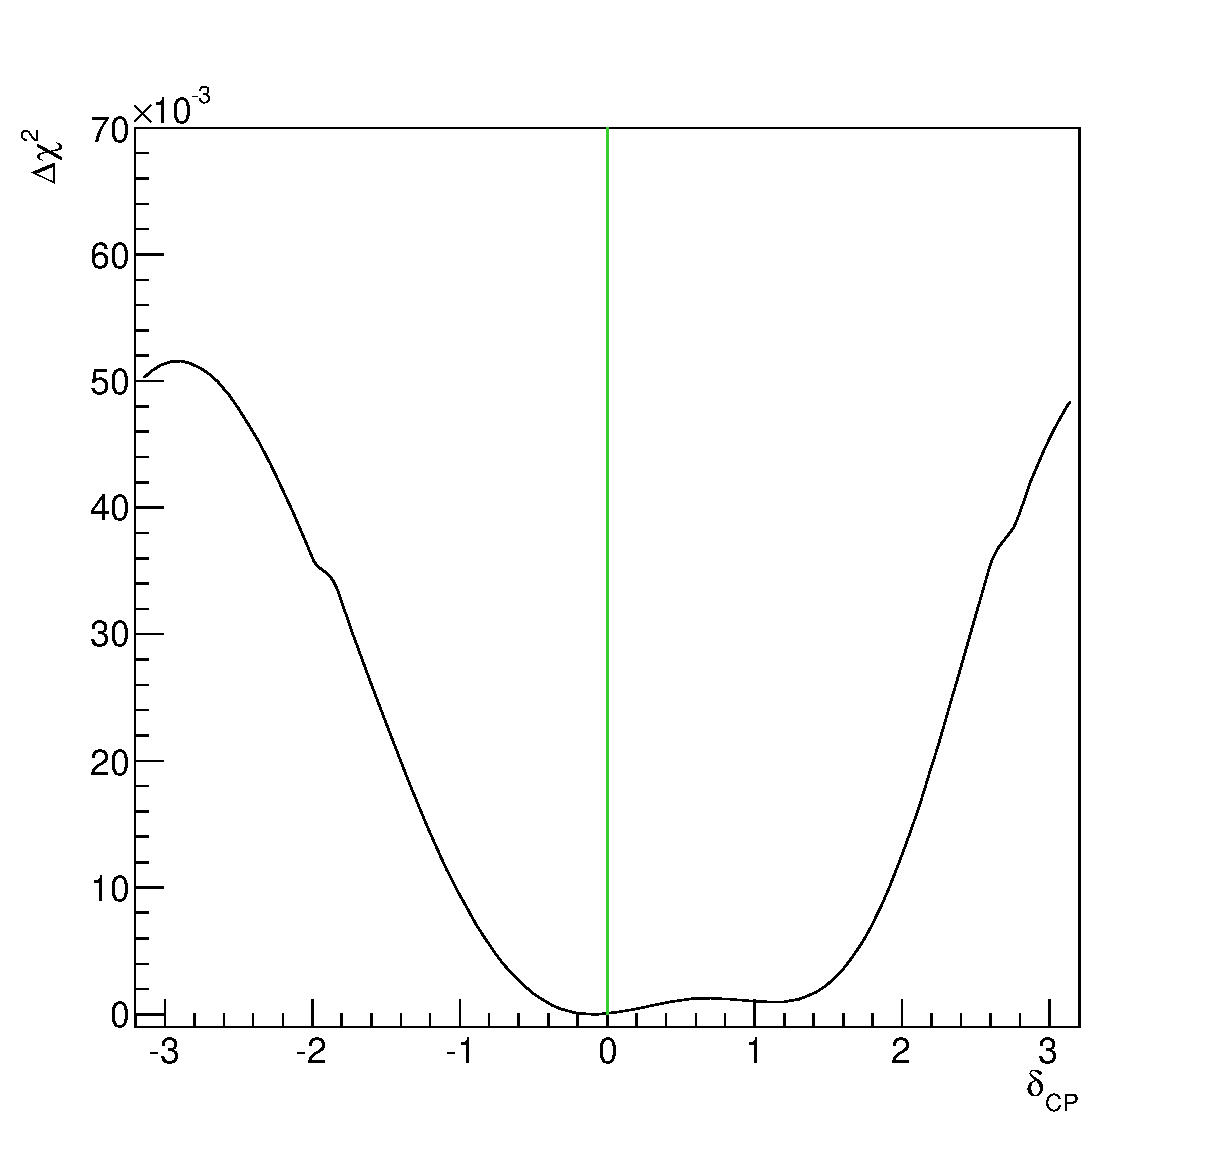
\includegraphics[width=9pc]{.//images/appendix/fake_dataset_fits/fake_dataset3_chisq_deltacp_global_min_new.eps}
\caption {
  $\Delta\chi^2$ as function of $\delta_{CP}$ for fake dataset \#2.
  At each point, $\chi^2$ was minimized with respect to 
  all oscillation parameters not shown (and not considered to be fixed)
  and all relevant nuisance parameters.
}
\label{fig:toymc2_dchisq_deltacp}
\end{minipage}

\vfill
\vspace*{0.7cm}

\begin{minipage}[t]{0.48\linewidth}
\center
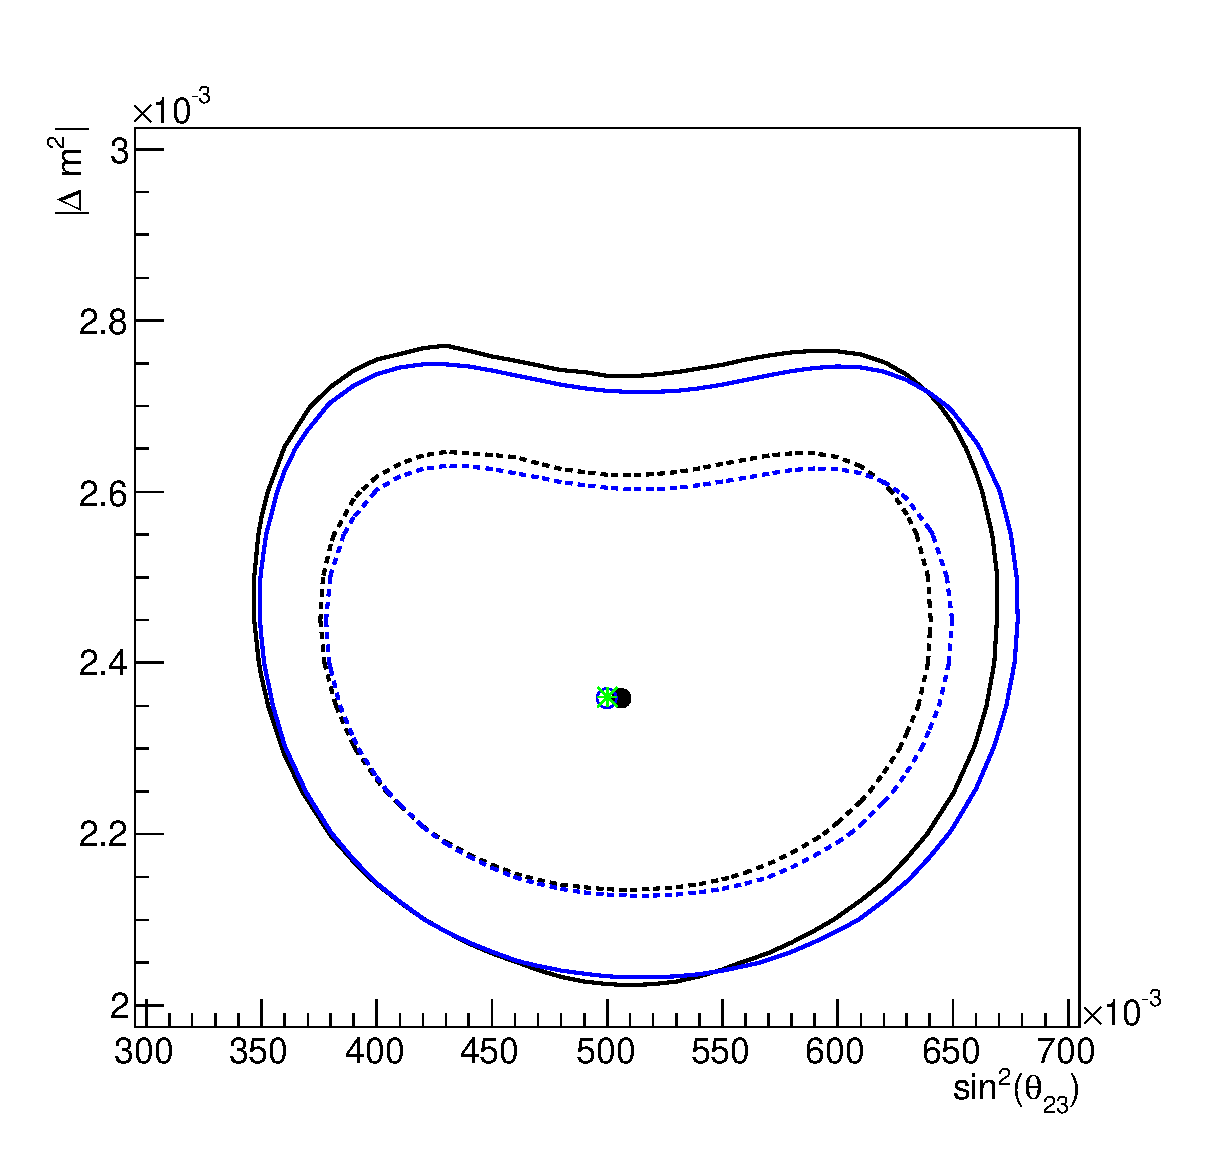
\includegraphics[width=15pc]{./images/appendix/fake_dataset_fits/fake_dataset3_chisq_theta23_dm23sq_global_min_new.eps}
\caption {
  68\% and 90\% CL regions in ($sin^{2}\theta_{23}$, $|\Delta m^{2}|$) space for fake dataset \#2.
  At each point, $\chi^2$ was minimized with respect to 
  $\sin^{2}\theta_{13}$, $\delta_{CP}$
  and all relevant nuisance parameters for the joint analysis (black)
  and with respect to all relevant nuisance parameters for the disappearance analysis (blue).
}
\label{fig:toymc2_confreg_sinsqtheta23_Dmsq}
\end{minipage}
\hspace{0.03\linewidth}
\begin{minipage}[t]{0.48\linewidth}
\center
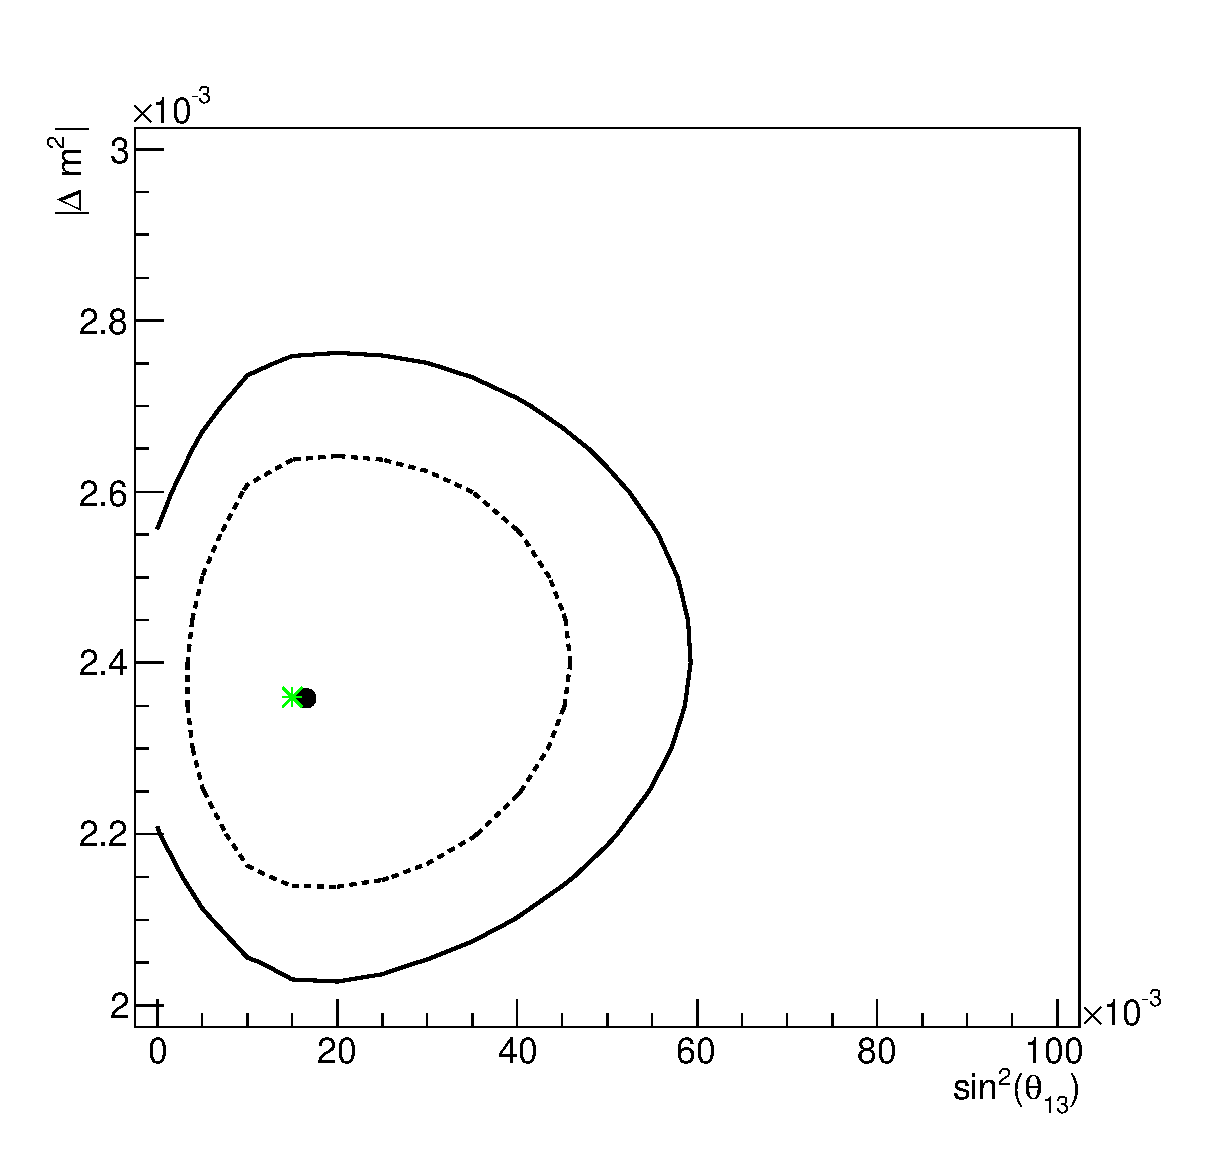
\includegraphics[width=15pc]{./images/appendix/fake_dataset_fits/fake_dataset3_chisq_theta13_dm23sq_global_min_new.eps}
\caption {
  68\% and 90\% CL regions in ($sin^{2}\theta_{13}$, $|\Delta m^{2}|$) space for fake dataset \#2.
  At each point, $\chi^2$ was minimized with respect to 
  all oscillation parameters not shown (and not considered to be fixed)
  and all relevant nuisance parameters.
}
\label{fig:toymc2_confreg_sinsqtheta13_Dmsq}
\end{minipage}

\vfill
\vspace*{0.7cm}

\begin{minipage}[t]{0.48\linewidth}
\center
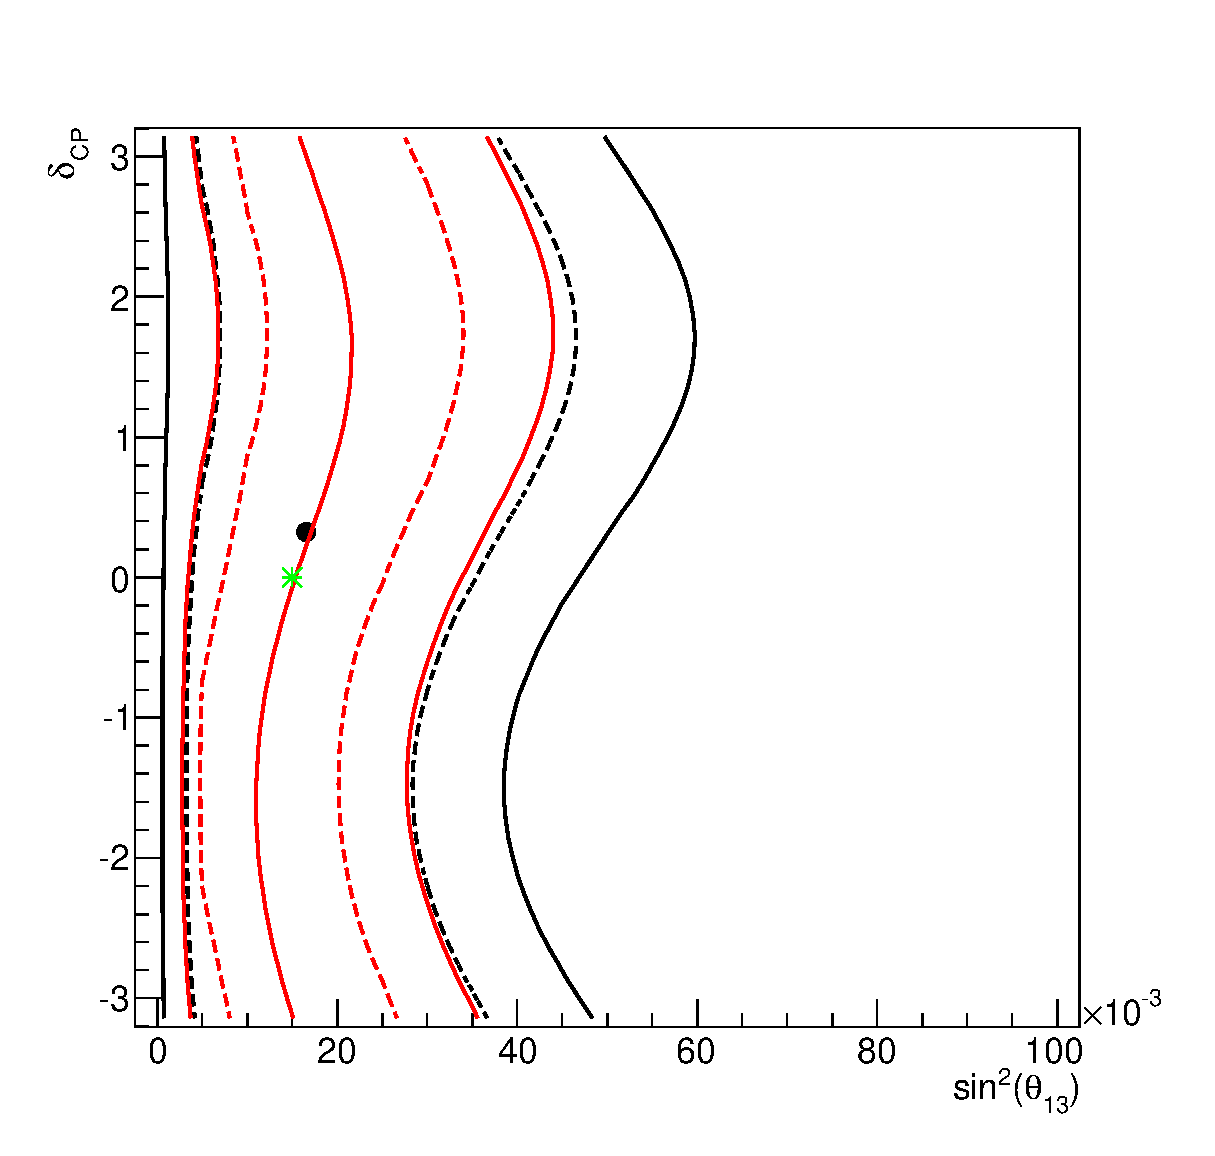
\includegraphics[width=15pc]{./images/appendix/fake_dataset_fits/fake_dataset3_chisq_theta13_deltacp_global_min_new.eps}
\caption {
  68\% and 90\% CL regions in ($sin^{2}\theta_{13}$, $\delta_{CP}$) space for fake dataset \#2.
  At each point, $\chi^2$ was minimized with respect to 
  $|\Delta m^{2}|$, $\sin^{2}\theta_{23}$
  and all relevant nuisance parameters for the joint analysis (black)
  and with respect to all relevant nuisance parameters for the appearance analysis (red).
  Notice that different methods are used to
  construct confidence regions for the joint analysis (global minimum) and for the 
  stand-alone appearance analysis (raster scan).
}
\label{fig:toymc2_confreg_sinsqtheta13_deltacp}
\end{minipage}
\hspace{0.03\linewidth}
\begin{minipage}[t]{0.48\linewidth}
\center
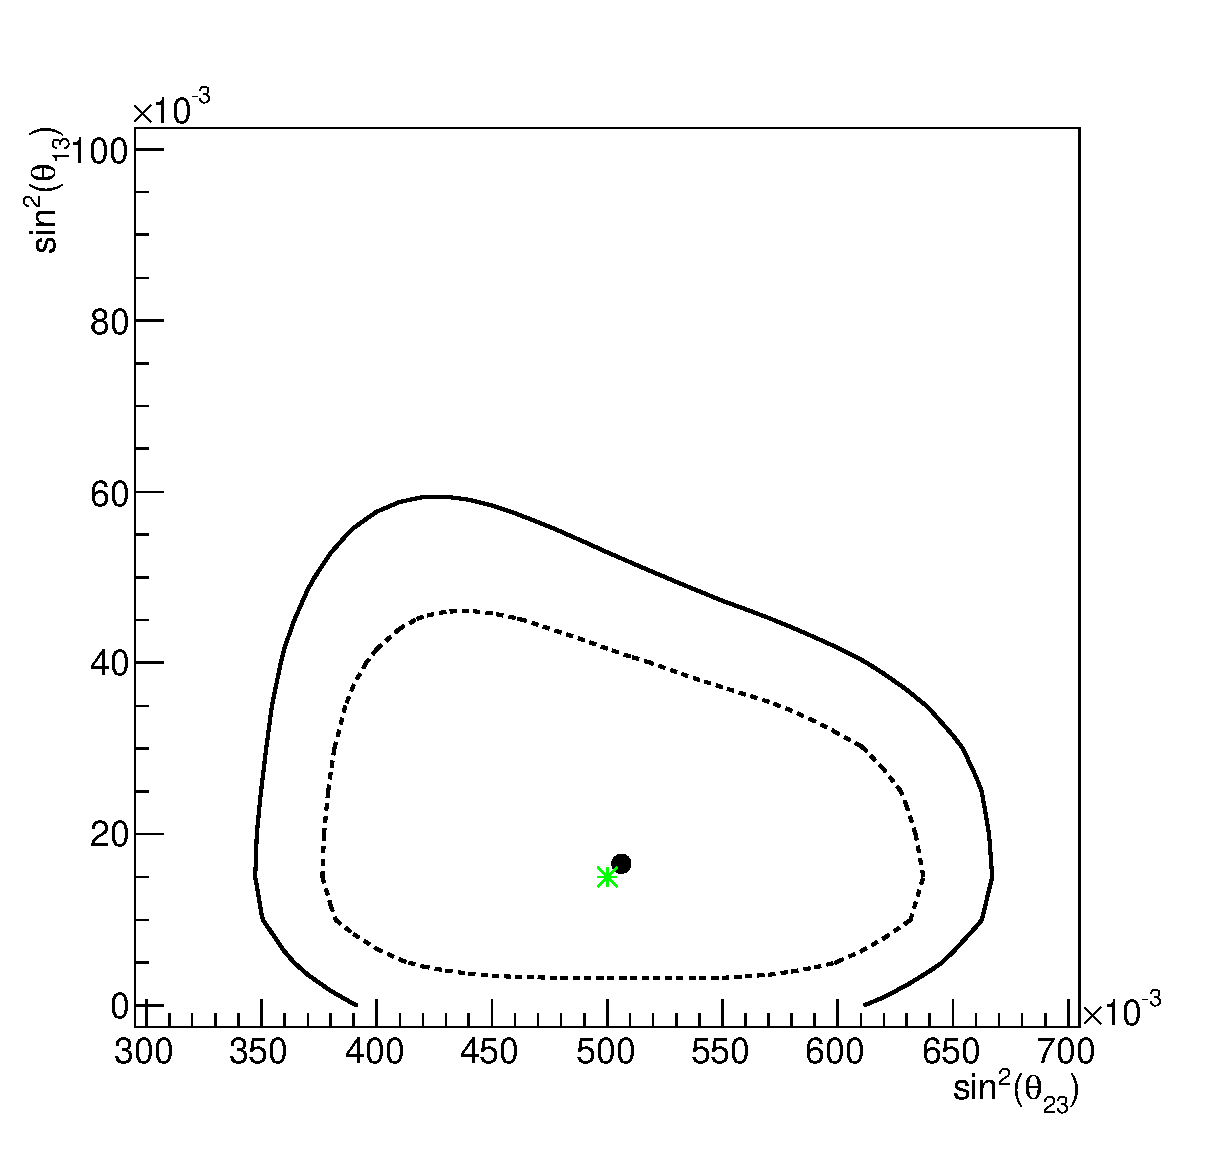
\includegraphics[width=15pc]{./images/appendix/fake_dataset_fits/fake_dataset3_chisq_theta13_theta23_global_min_new.eps}
\caption {
  68\% and 90\% CL regions in ($sin^{2}\theta_{23}$, $sin^{2}\theta_{13}$) space for fake dataset \#2.
  At each point, $\chi^2$ was minimized with respect to 
  all oscillation parameters not shown (and not considered to be fixed)
  and all relevant nuisance parameters.
}
\label{fig:toymc2_confreg_sinsqtheta23_sinsqtheta13}
\end{minipage}

\end{figure*}

%
%
% ..............................................
% Fake dataset #3
%
%

\clearpage

%
% delta\chisq and contours
%

\begin{figure*}[htb]

\begin{minipage}[t]{0.22\linewidth}
\center
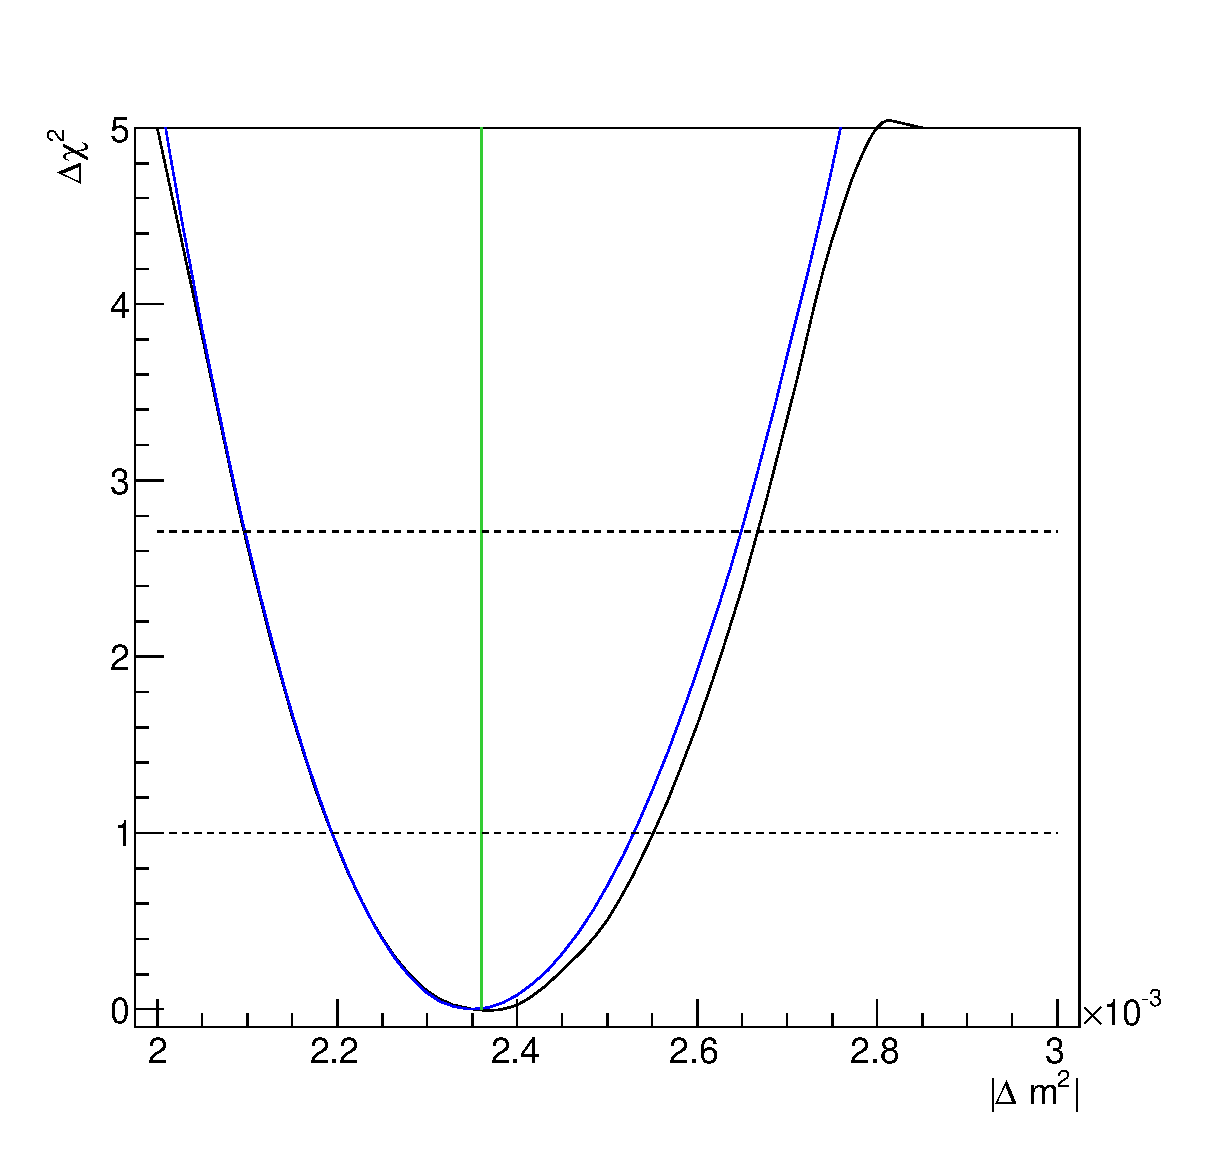
\includegraphics[width=9pc]{./images/appendix/fake_dataset_fits/fake_dataset5_chisq_dm23sq_global_min_new.eps}
\caption {
  $\Delta\chi^2$ as function of $|\Delta m^{2}|$ for fake dataset \#3.
  At each point, $\chi^2$ was minimized with respect to 
  $\sin^{2}\theta_{23}$, $\sin^{2}\theta_{13}$, $\delta_{CP}$
  and all relevant nuisance parameters for the joint analysis (black)
  and with respect to $\sin^{2}\theta_{23}$ and all relevant nuisance
  parameters for the disappearance analysis (blue).
}
\label{fig:toymc3_dchisq_Dmsq}
\end{minipage}
\hspace{0.02\linewidth}
\begin{minipage}[t]{0.22\linewidth}
\center
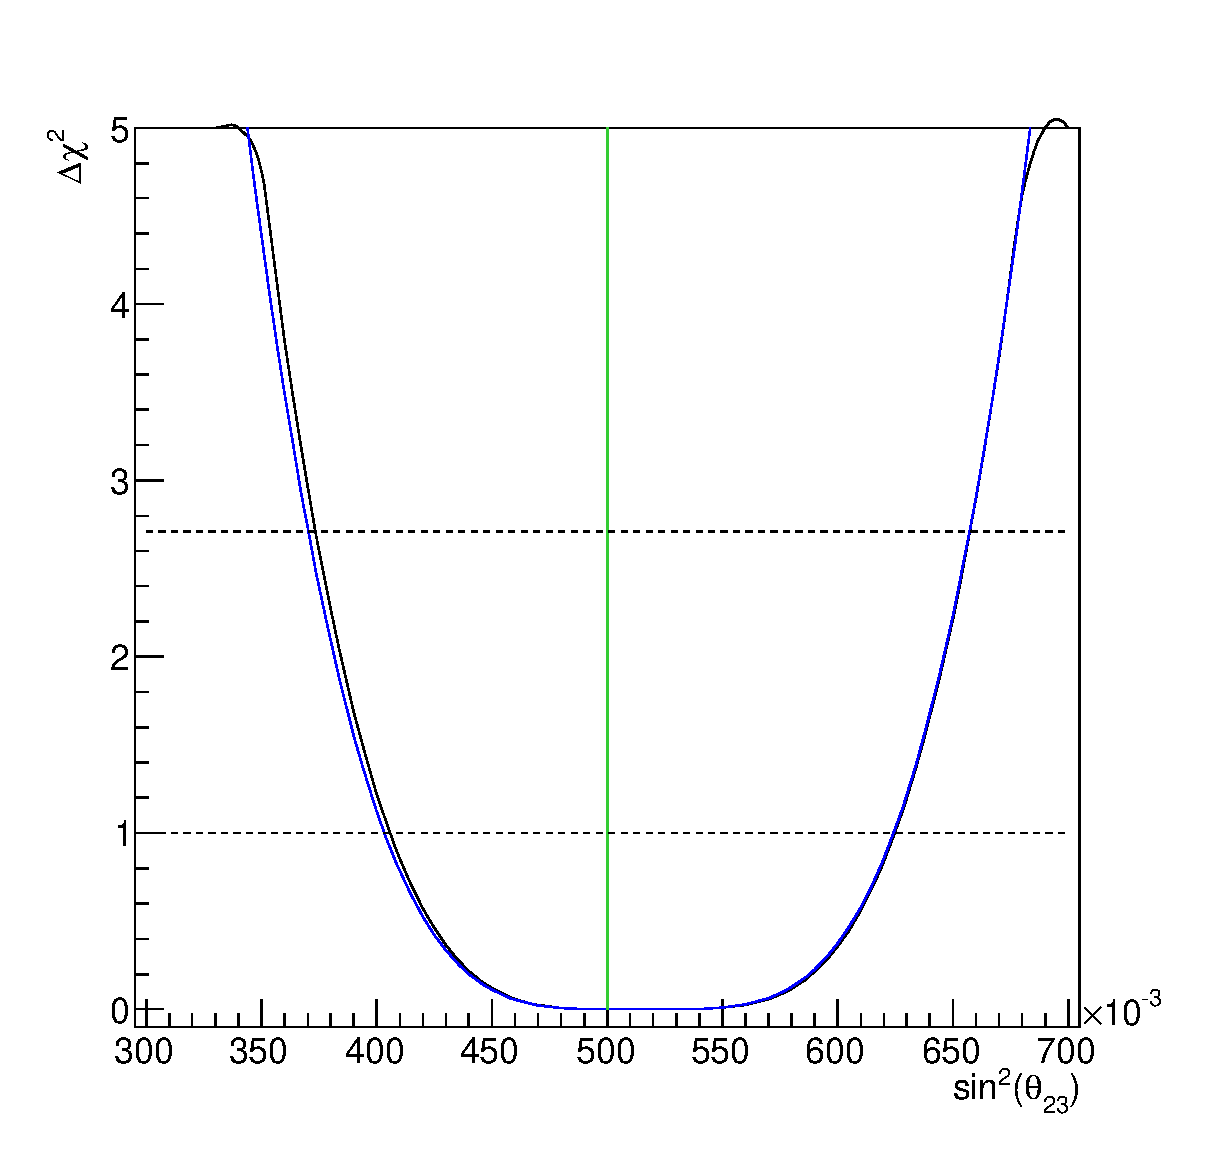
\includegraphics[width=9pc]{./images/appendix/fake_dataset_fits/fake_dataset5_chisq_theta23_global_min_new.eps}
\caption {
  $\Delta\chi^2$ as function of $sin^{2}\theta_{23}$ for fake dataset \#3.
  At each point, $\chi^2$ was minimized with respect to 
  $|\Delta m^{2}|$, $\sin^{2}\theta_{13}$, $\delta_{CP}$
  and all relevant nuisance parameters for the joint analysis (black)
  and with respect to $\sin^{2}\theta_{23}$ and all relevant nuisance
  parameters for the disappearance analysis (blue).
}
\label{fig:toymc3_dchisq_sinsqtheta23}
\end{minipage}
\hspace{0.02\linewidth}
\begin{minipage}[t]{0.22\linewidth}
\center
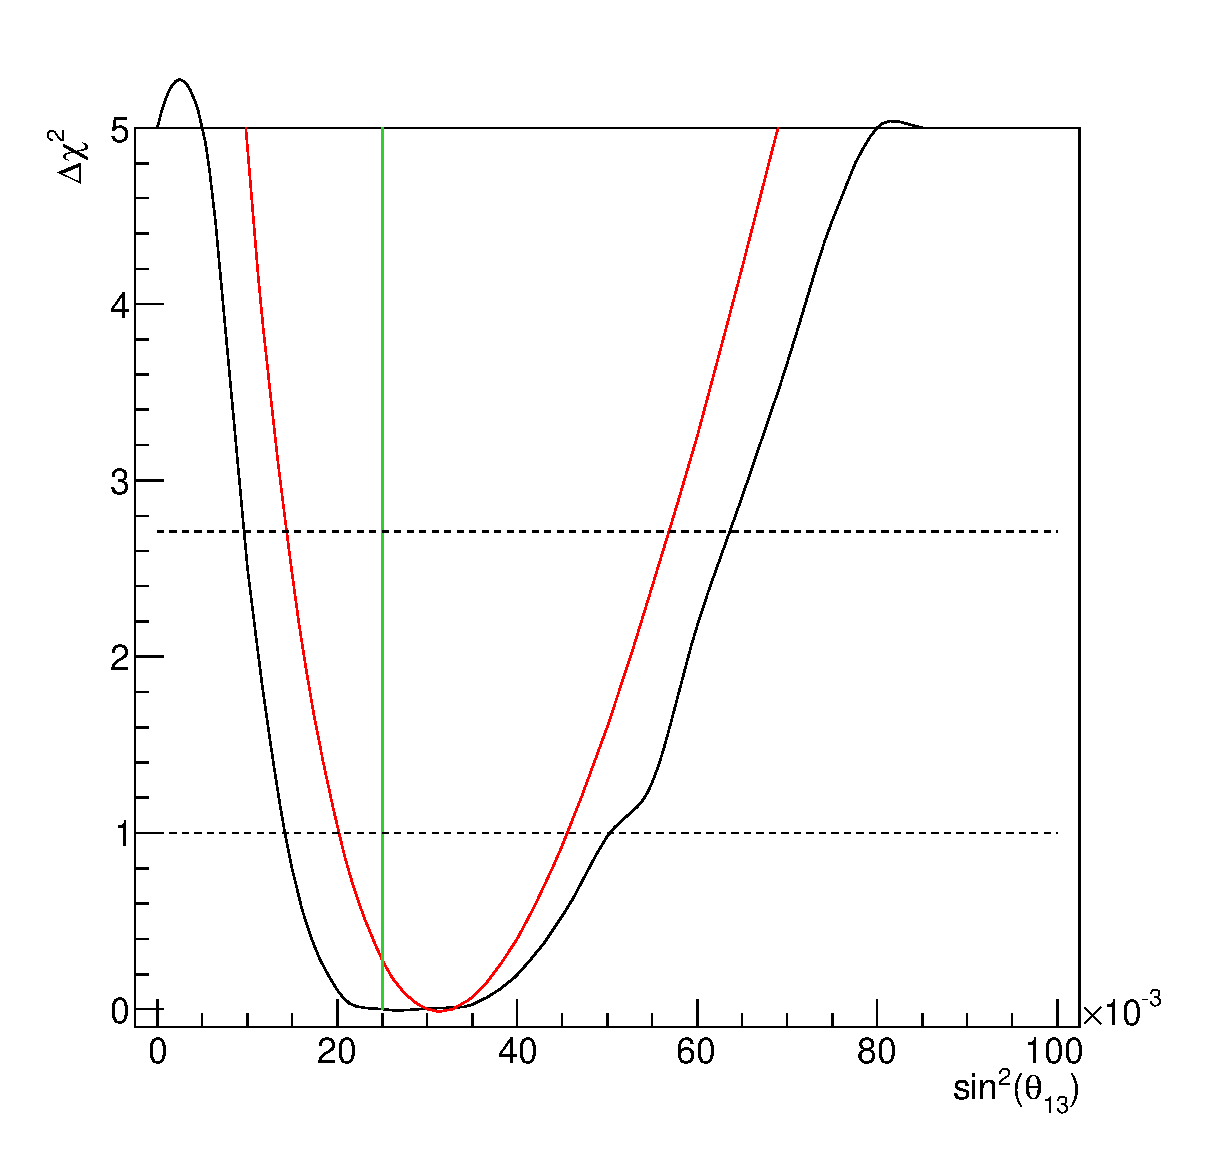
\includegraphics[width=9pc]{./images/appendix/fake_dataset_fits/fake_dataset5_chisq_theta13_global_min_new.eps}
\caption {
  $\Delta\chi^2$ as function of $sin^{2}\theta_{13}$ for fake dataset \#3.
  At each point, $\chi^2$ was minimized with respect to 
  $\sin^{2}\theta_{23}$, $\sin^{2}\theta_{13}$, $\delta_{CP}$
  and all relevant nuisance parameters for the joint analysis (black)
  and with respect to all relevant nuisance parameters 
  ($\delta_{CP}$ is fixed to 0) for the appearance analysis (red).
}
\label{fig:toymc3_dchisq_sinsqtheta13}
\end{minipage}
\hspace{0.02\linewidth}
\begin{minipage}[t]{0.22\linewidth}
\center
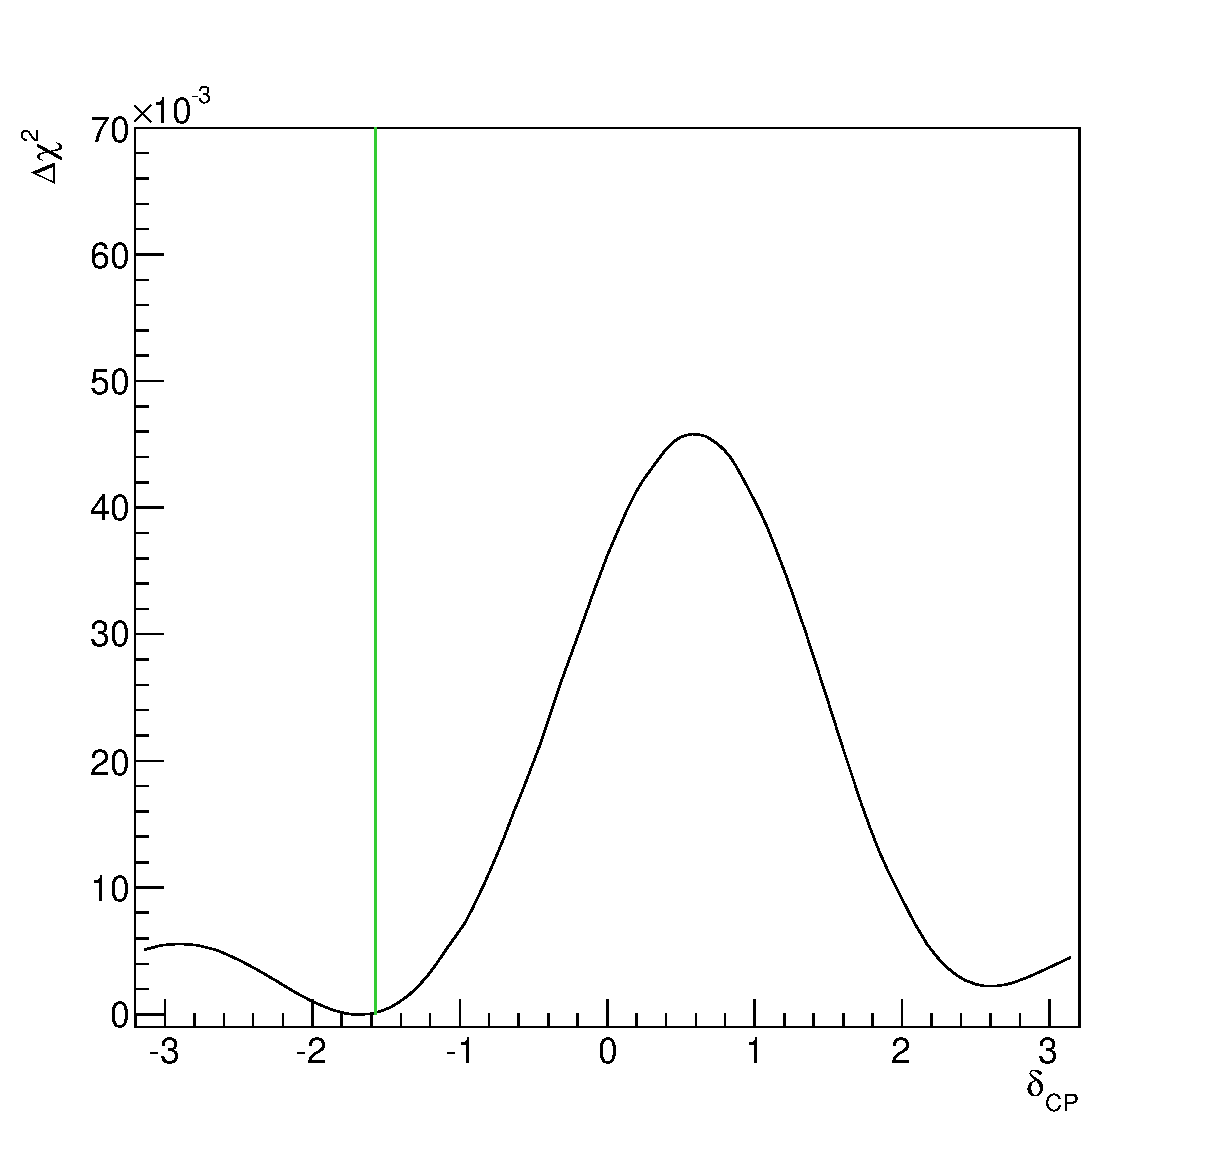
\includegraphics[width=9pc]{.//images/appendix/fake_dataset_fits/fake_dataset5_chisq_deltacp_global_min_new.eps}
\caption {
  $\Delta\chi^2$ as function of $\delta_{CP}$ for fake dataset \#3.
  At each point, $\chi^2$ was minimized with respect to 
  all oscillation parameters not shown (and not considered to be fixed)
  and all relevant nuisance parameters.
}
\label{fig:toymc3_dchisq_deltacp}
\end{minipage}
\vfill
\vspace*{0.7cm}
\begin{minipage}[t]{0.48\linewidth}
\center
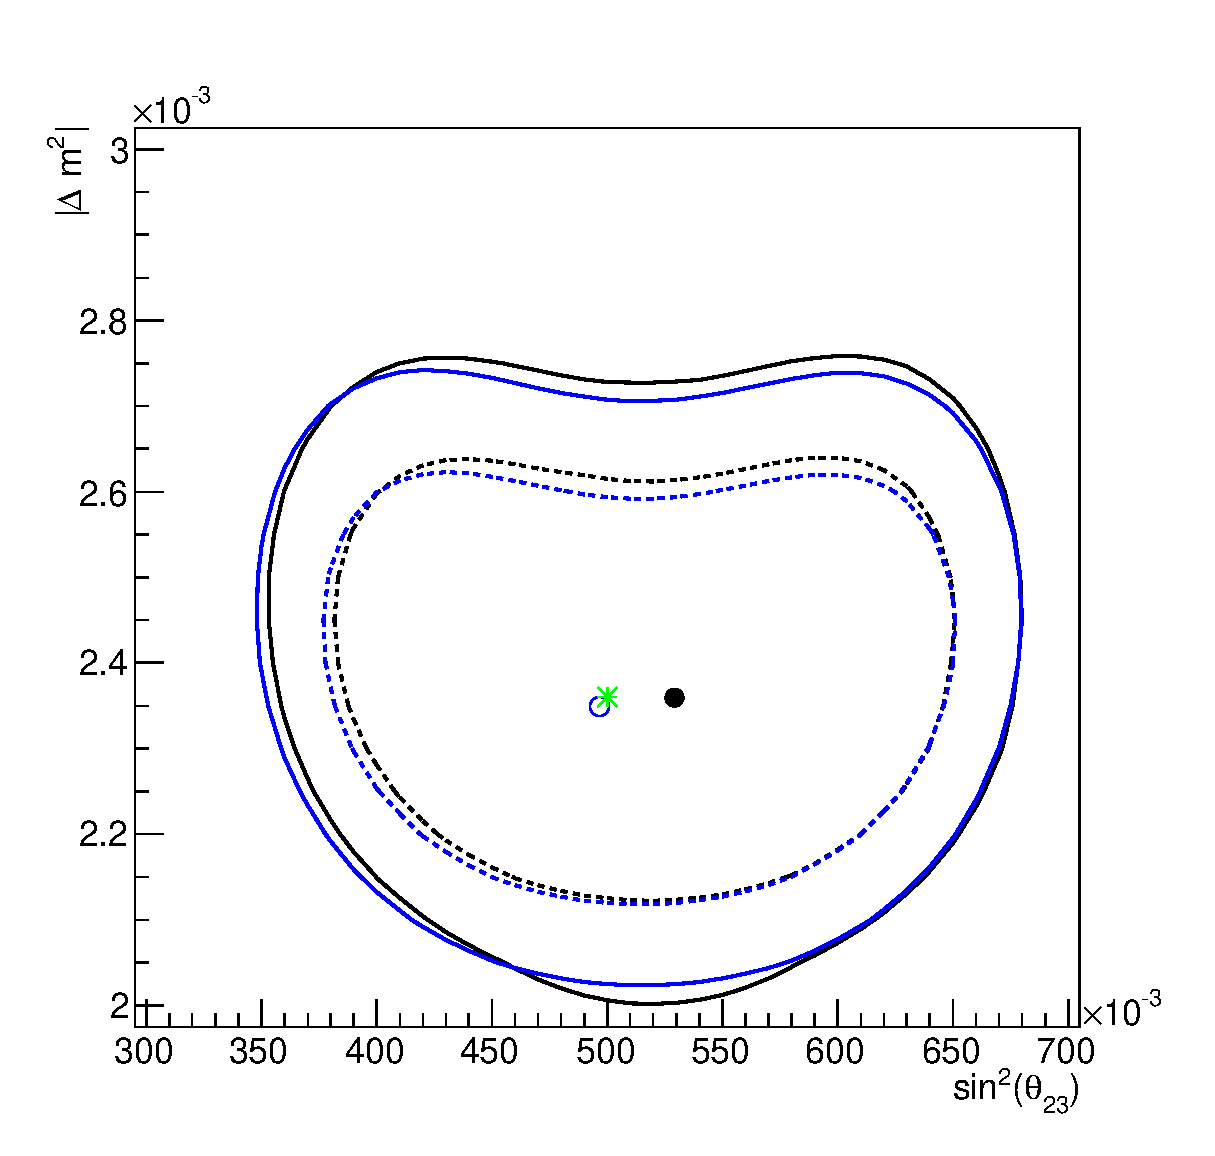
\includegraphics[width=15pc]{./images/appendix/fake_dataset_fits/fake_dataset5_chisq_theta23_dm23sq_global_min_new.eps}
\caption {
  68\% and 90\% CL regions in ($sin^{2}\theta_{23}$, $|\Delta m^{2}|$) space for fake dataset \#3.
  At each point, $\chi^2$ was minimized with respect to 
  $\sin^{2}\theta_{13}$, $\delta_{CP}$
  and all relevant nuisance parameters for the joint analysis (black)
  and with respect to all relevant nuisance parameters for the disappearance analysis (blue).
}
\label{fig:toymc3_confreg_sinsqtheta23_Dmsq}
\end{minipage}
\hspace{0.03\linewidth}
\begin{minipage}[t]{0.48\linewidth}
\center
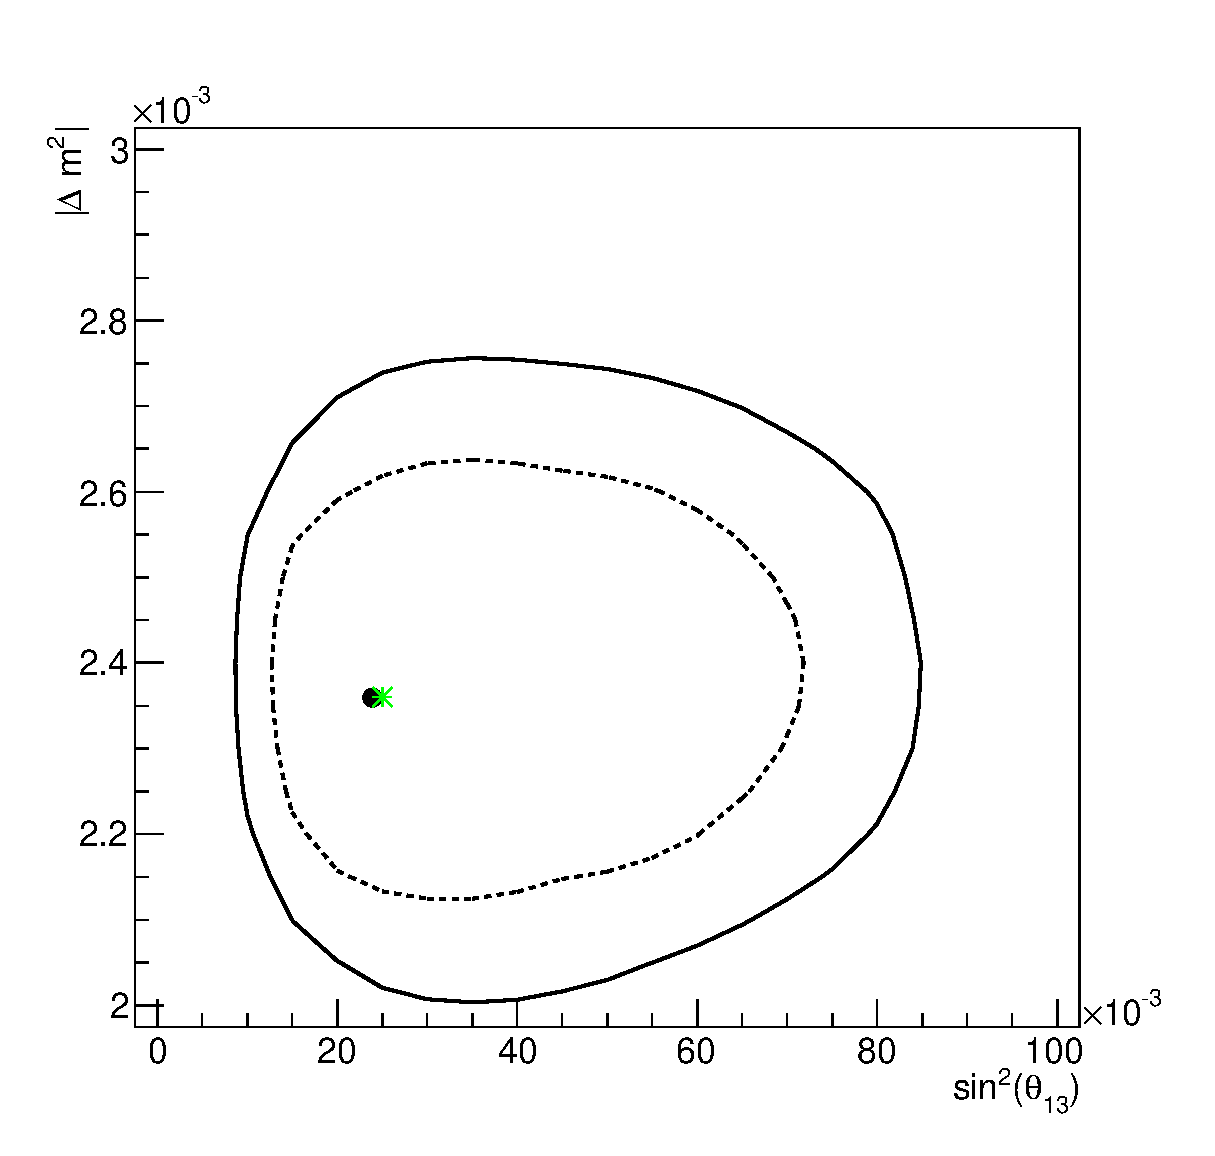
\includegraphics[width=15pc]{./images/appendix/fake_dataset_fits/fake_dataset5_chisq_theta13_dm23sq_global_min_new.eps}
\caption {
  68\% and 90\% CL regions in ($sin^{2}\theta_{13}$, $|\Delta m^{2}|$) space for fake dataset \#3.
  At each point, $\chi^2$ was minimized with respect to 
  all oscillation parameters not shown (and not considered to be fixed)
  and all relevant nuisance parameters.
}
\label{fig:toymc3_confreg_sinsqtheta13_Dmsq}
\end{minipage}
\vfill
\vspace*{0.7cm}
\begin{minipage}[t]{0.48\linewidth}
\center
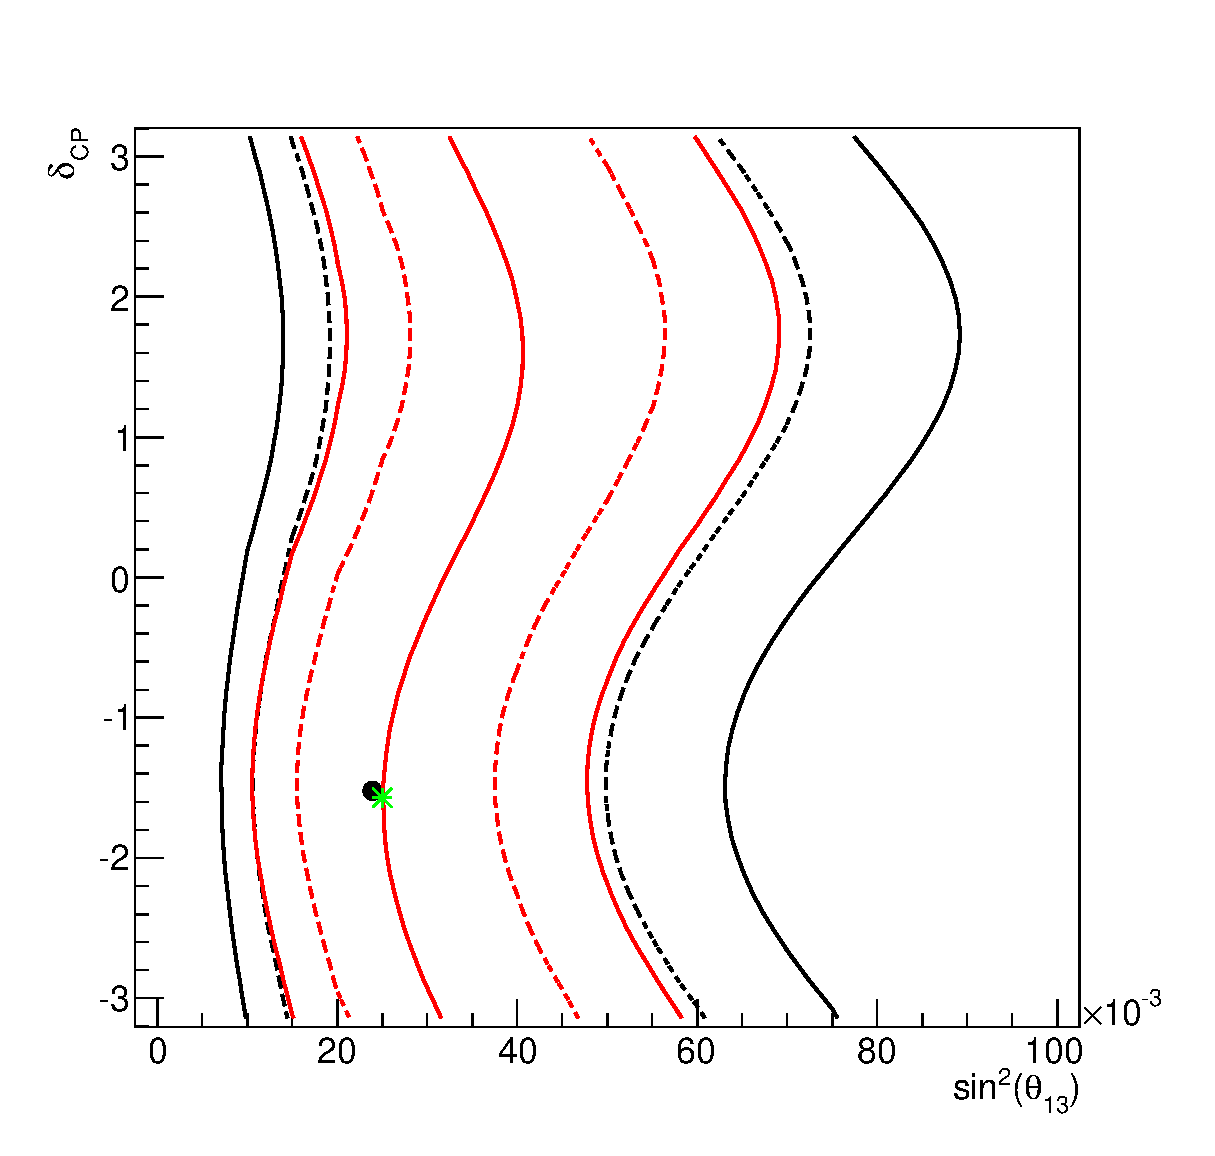
\includegraphics[width=15pc]{./images/appendix/fake_dataset_fits/fake_dataset5_chisq_theta13_deltacp_global_min_new.eps}
\caption {
  68\% and 90\% CL regions in ($sin^{2}\theta_{13}$, $\delta_{CP}$) space for fake dataset \#3.
  At each point, $\chi^2$ was minimized with respect to 
  $|\Delta m^{2}|$, $\sin^{2}\theta_{23}$
  and all relevant nuisance parameters for the joint analysis (black)
  and with respect to all relevant nuisance parameters for the appearance analysis (red).
  Notice that different methods are used to
  construct confidence regions for the joint analysis (global minimum) and for the 
  stand-alone appearance analysis (raster scan).
}
\label{fig:toymc3_confreg_sinsqtheta13_deltacp}
\end{minipage}
\hspace{0.03\linewidth}
\begin{minipage}[t]{0.48\linewidth}
\center
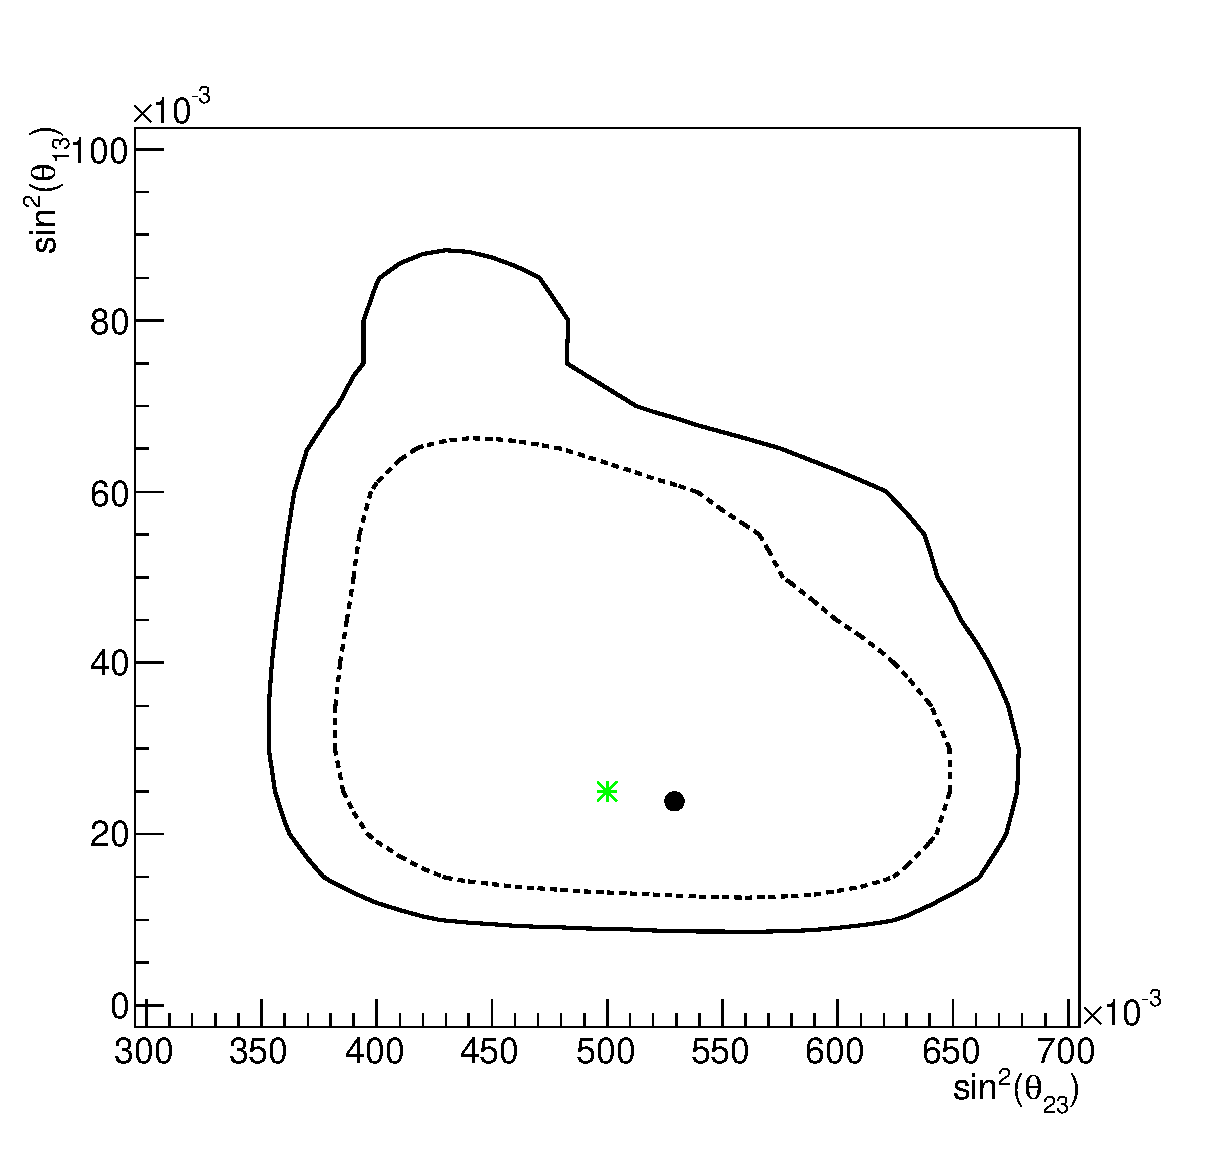
\includegraphics[width=15pc]{./images/appendix/fake_dataset_fits/fake_dataset5_chisq_theta13_theta23_global_min_new.eps}
\caption {
  68\% and 90\% CL regions in ($sin^{2}\theta_{23}$, $sin^{2}\theta_{13}$) space for fake dataset \#3.
  At each point, $\chi^2$ was minimized with respect to 
  all oscillation parameters not shown (and not considered to be fixed)
  and all relevant nuisance parameters.
}
\label{fig:toymc3_confreg_sinsqtheta23_sinsqtheta13}
\end{minipage}

\end{figure*}

%
%
% ..............................................
% Fake dataset #4
%
%

\clearpage

%
% delta\chisq and contours
%

\begin{figure*}[htb]

\begin{minipage}[t]{0.22\linewidth}
\center
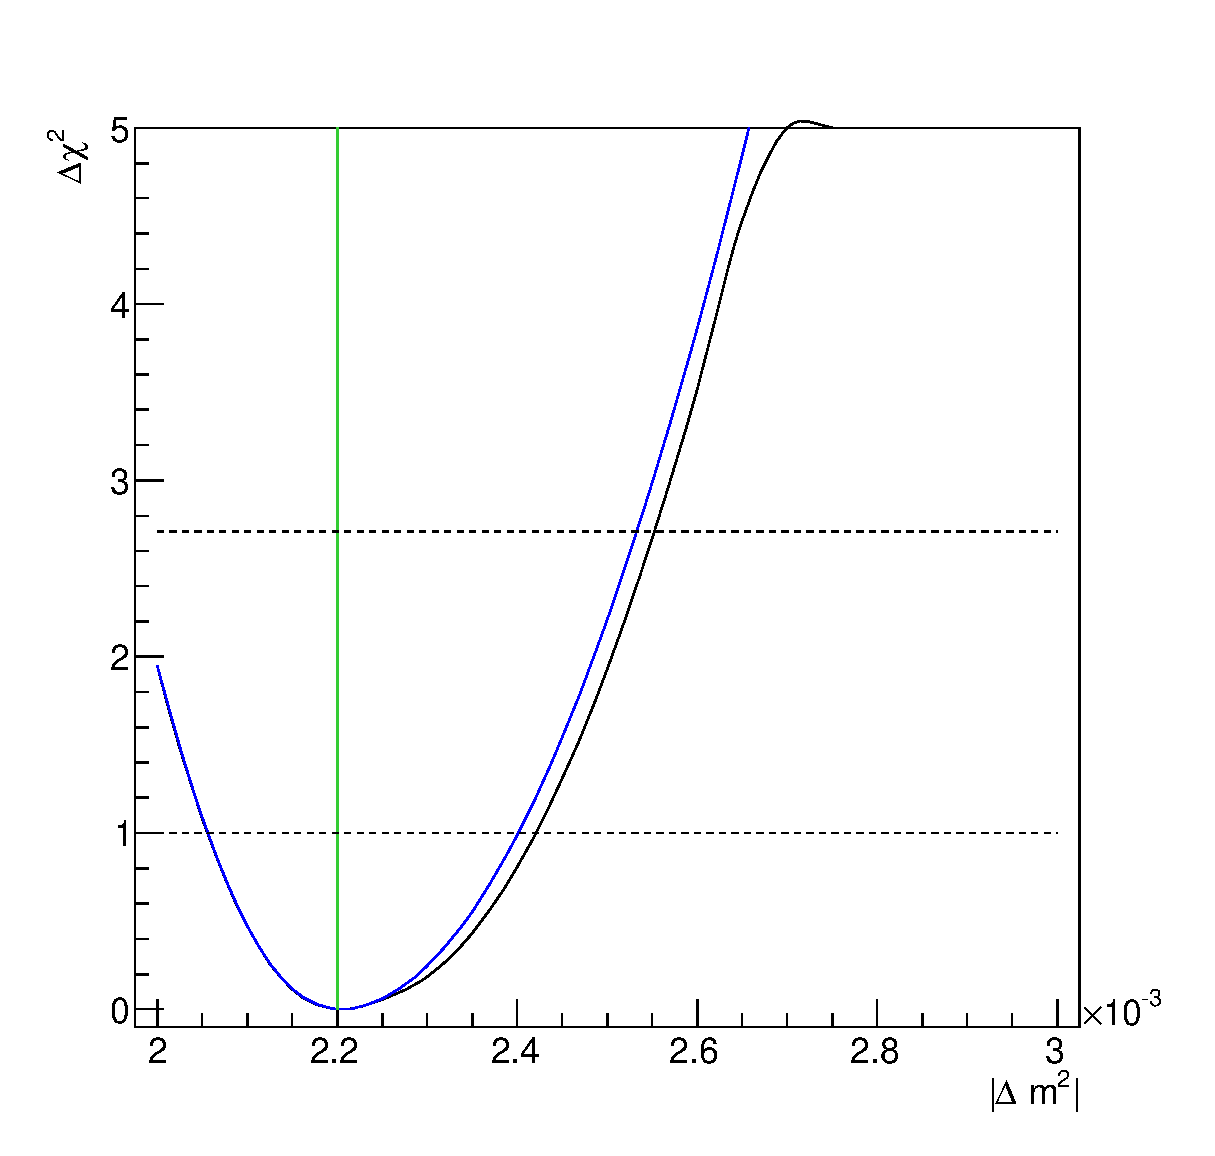
\includegraphics[width=9pc]{./images/appendix/fake_dataset_fits/fake_dataset7_chisq_dm23sq_global_min_new.eps}
\caption {
  $\Delta\chi^2$ as function of $|\Delta m^{2}|$ for fake dataset \#4.
  At each point, $\chi^2$ was minimized with respect to 
  $\sin^{2}\theta_{23}$, $\sin^{2}\theta_{13}$, $\delta_{CP}$
  and all relevant nuisance parameters for the joint analysis (black)
  and with respect to $\sin^{2}\theta_{23}$ and all relevant nuisance
  parameters for the disappearance analysis (blue).
}
\label{fig:toymc4_dchisq_Dmsq}
\end{minipage}
\hspace{0.02\linewidth}
\begin{minipage}[t]{0.22\linewidth}
\center
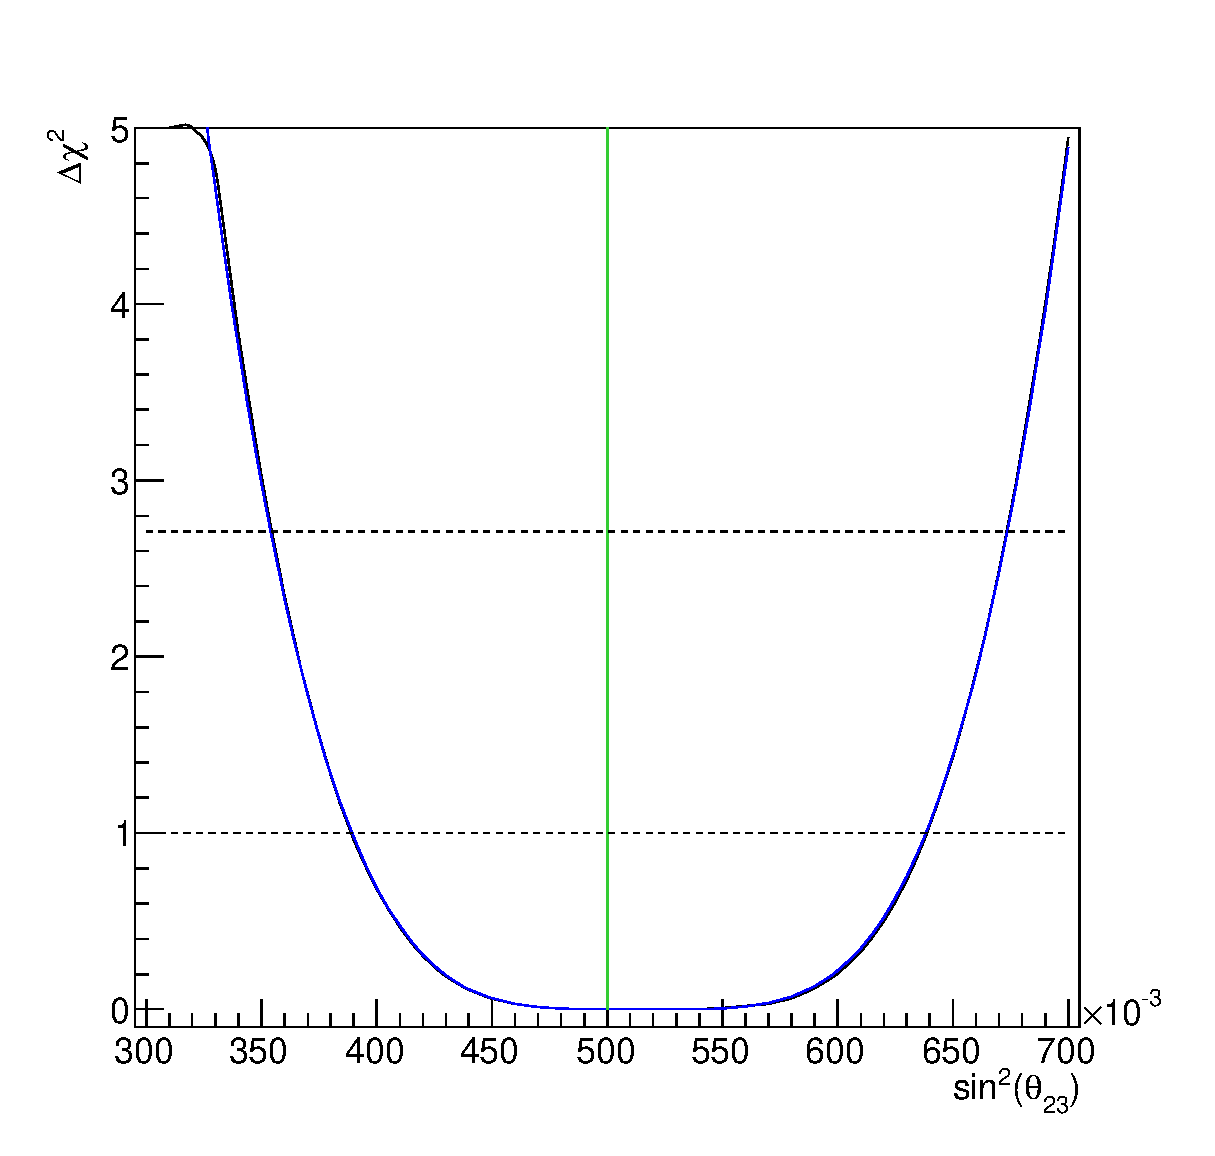
\includegraphics[width=9pc]{./images/appendix/fake_dataset_fits/fake_dataset7_chisq_theta23_global_min_new.eps}
\caption {
  $\Delta\chi^2$ as function of $sin^{2}\theta_{23}$ for fake dataset \#4.
  At each point, $\chi^2$ was minimized with respect to 
  $|\Delta m^{2}|$, $\sin^{2}\theta_{13}$, $\delta_{CP}$
  and all relevant nuisance parameters for the joint analysis (black)
  and with respect to $\sin^{2}\theta_{23}$ and all relevant nuisance
  parameters for the disappearance analysis (blue).
}
\label{fig:toymc4_dchisq_sinsqtheta23}
\end{minipage}
\hspace{0.02\linewidth}
\begin{minipage}[t]{0.22\linewidth}
\center
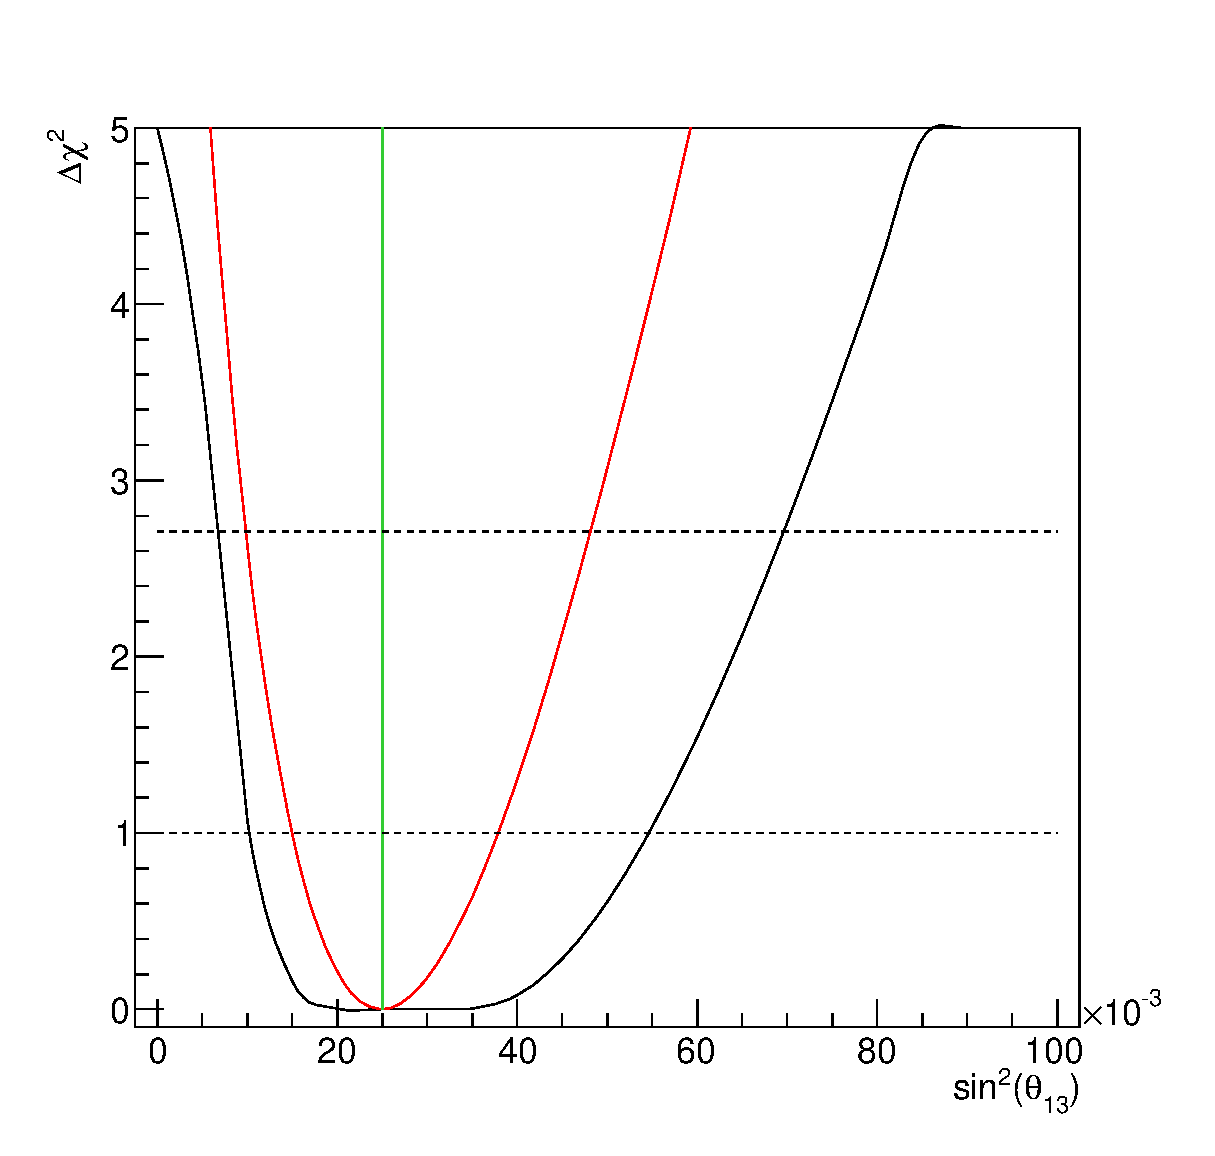
\includegraphics[width=9pc]{./images/appendix/fake_dataset_fits/fake_dataset7_chisq_theta13_global_min_new.eps}
\caption {
  $\Delta\chi^2$ as function of $sin^{2}\theta_{13}$ for fake dataset \#4.
  At each point, $\chi^2$ was minimized with respect to 
  $\sin^{2}\theta_{23}$, $\sin^{2}\theta_{13}$, $\delta_{CP}$
  and all relevant nuisance parameters for the joint analysis (black)
  and with respect to all relevant nuisance parameters 
  ($\delta_{CP}$ is fixed to 0) for the appearance analysis (red).
}
\label{fig:toymc4_dchisq_sinsqtheta13}
\end{minipage}
\hspace{0.02\linewidth}
\begin{minipage}[t]{0.22\linewidth}
\center
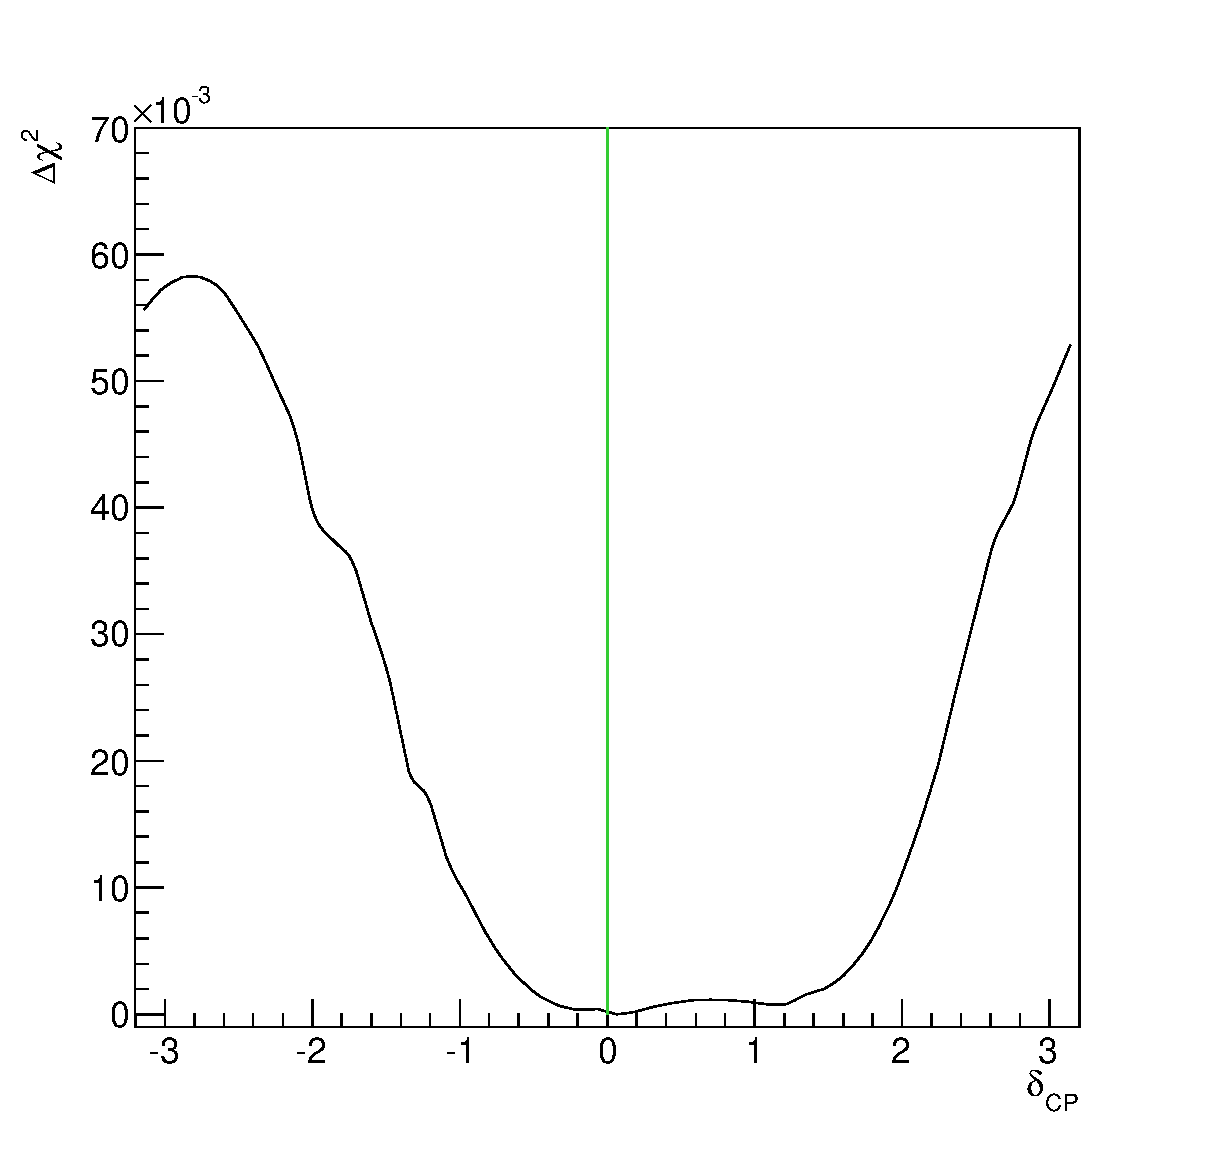
\includegraphics[width=9pc]{.//images/appendix/fake_dataset_fits/fake_dataset7_chisq_deltacp_global_min_new.eps}
\caption {
  $\Delta\chi^2$ as function of $\delta_{CP}$ for fake dataset \#4.
  At each point, $\chi^2$ was minimized with respect to 
  all oscillation parameters not shown (and not considered to be fixed)
  and all relevant nuisance parameters.
}
\label{fig:toymc4_dchisq_deltacp}
\end{minipage}

\vfill
\vspace*{0.7cm}

\begin{minipage}[t]{0.48\linewidth}
\center
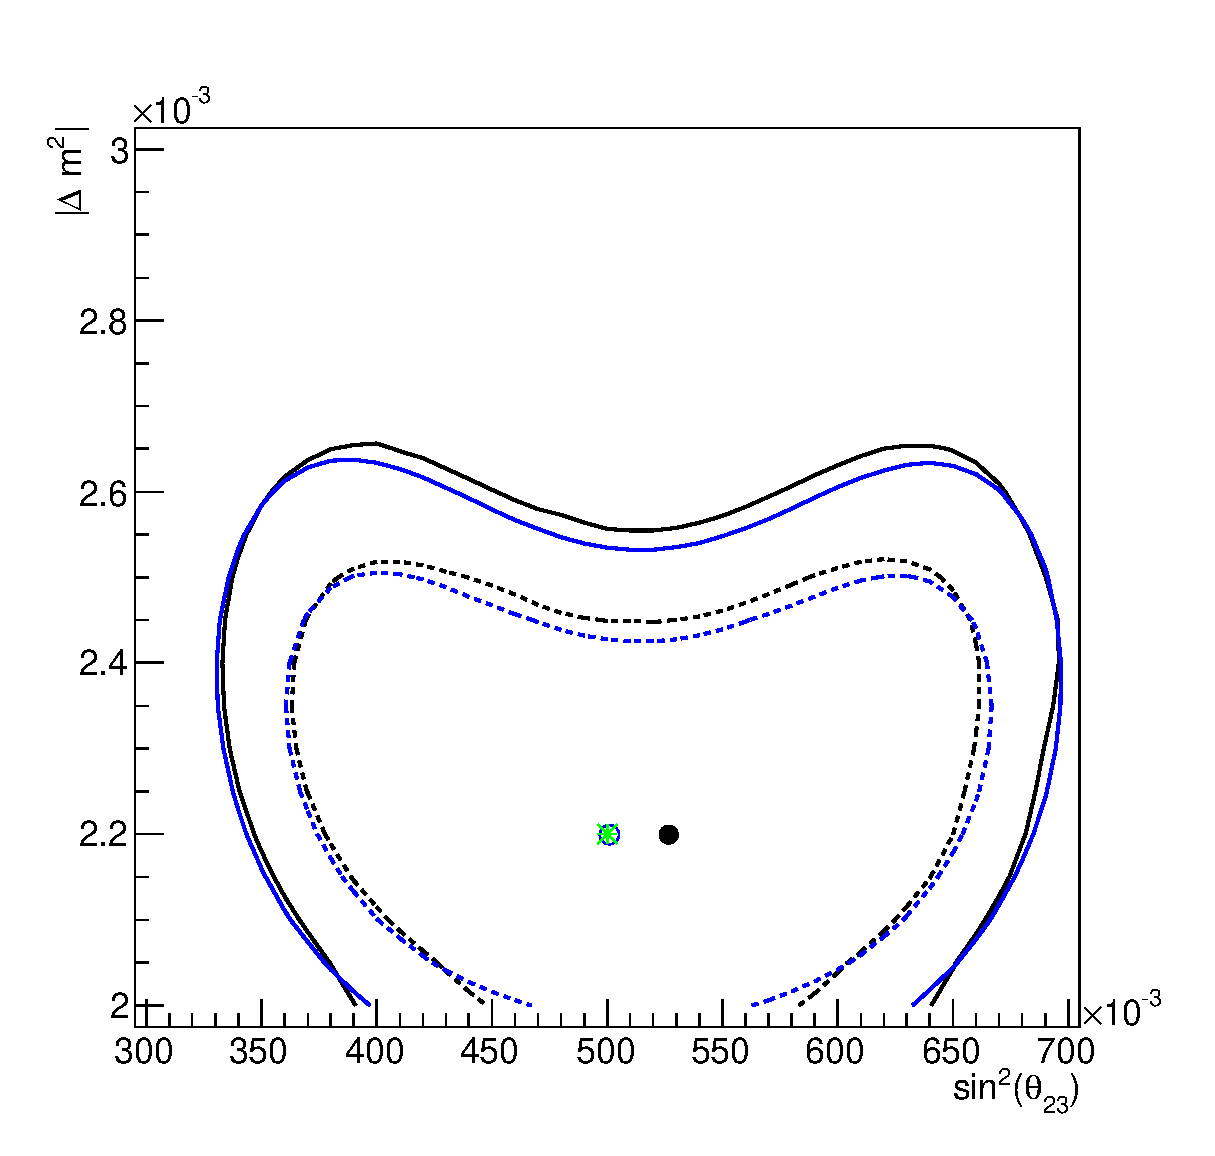
\includegraphics[width=15pc]{./images/appendix/fake_dataset_fits/fake_dataset7_chisq_theta23_dm23sq_global_min_new.eps}
\caption {
  68\% and 90\% CL regions in ($sin^{2}\theta_{23}$, $|\Delta m^{2}|$) space for fake dataset \#4.
  At each point, $\chi^2$ was minimized with respect to 
  $\sin^{2}\theta_{13}$, $\delta_{CP}$
  and all relevant nuisance parameters for the joint analysis (black)
  and with respect to all relevant nuisance parameters for the disappearance analysis (blue).
}
\label{fig:toymc4_confreg_sinsqtheta23_Dmsq}
\end{minipage}
\hspace{0.03\linewidth}
\begin{minipage}[t]{0.48\linewidth}
\center
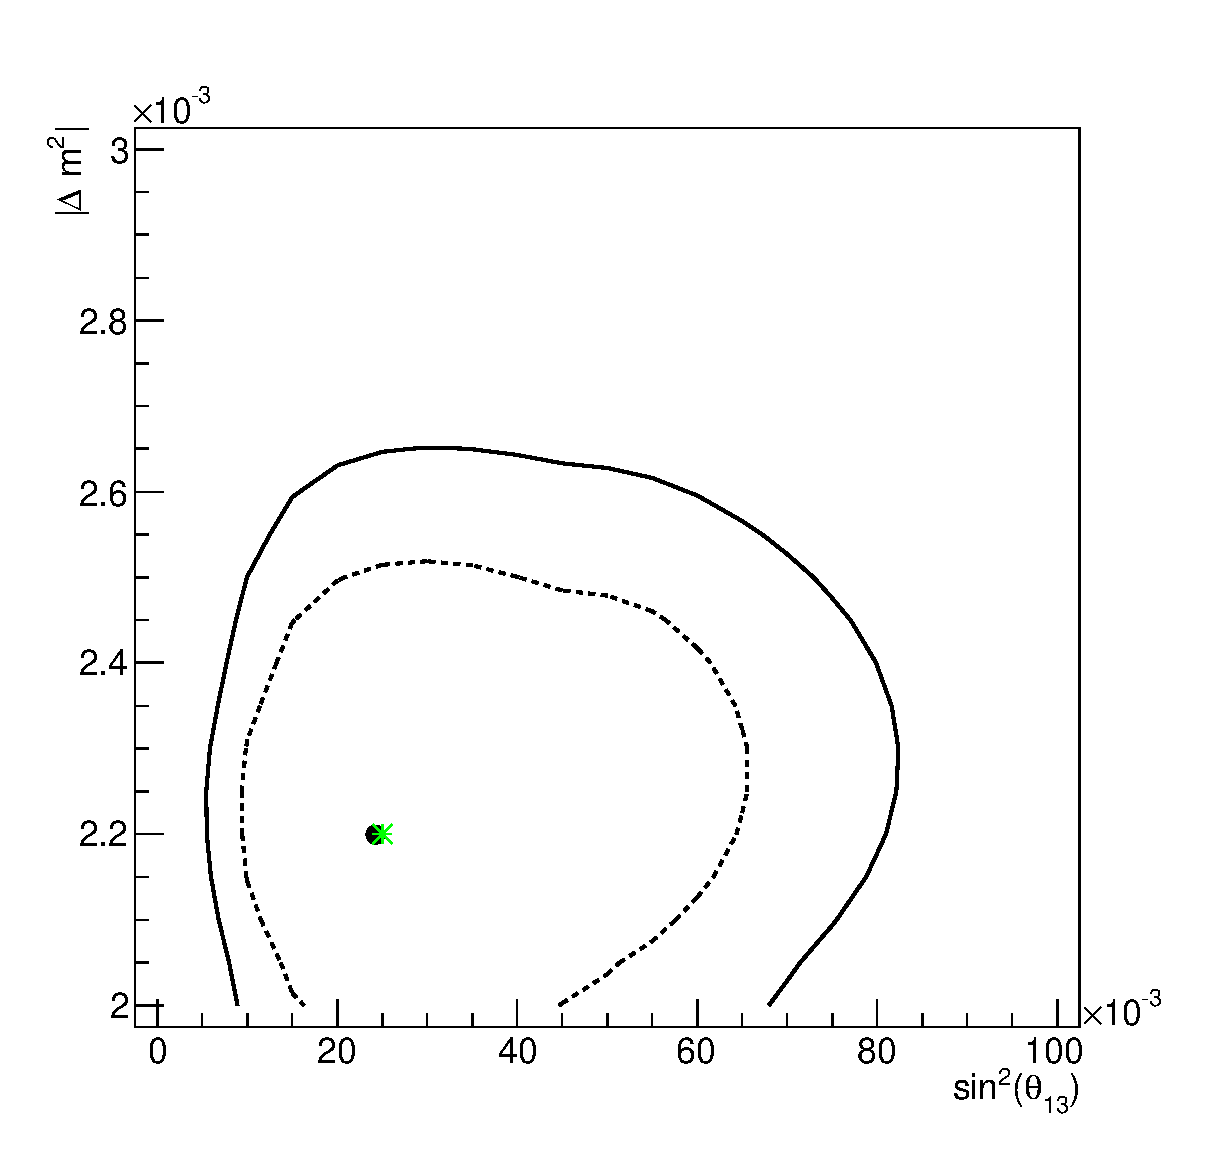
\includegraphics[width=15pc]{./images/appendix/fake_dataset_fits/fake_dataset7_chisq_theta13_dm23sq_global_min_new.eps}
\caption {
  68\% and 90\% CL regions in ($sin^{2}\theta_{13}$, $|\Delta m^{2}|$) space for fake dataset \#4.
  At each point, $\chi^2$ was minimized with respect to 
  all oscillation parameters not shown (and not considered to be fixed)
  and all relevant nuisance parameters.
}
\label{fig:toymc4_confreg_sinsqtheta13_Dmsq}
\end{minipage}

\vfill
\vspace*{0.7cm}

\begin{minipage}[t]{0.48\linewidth}
\center
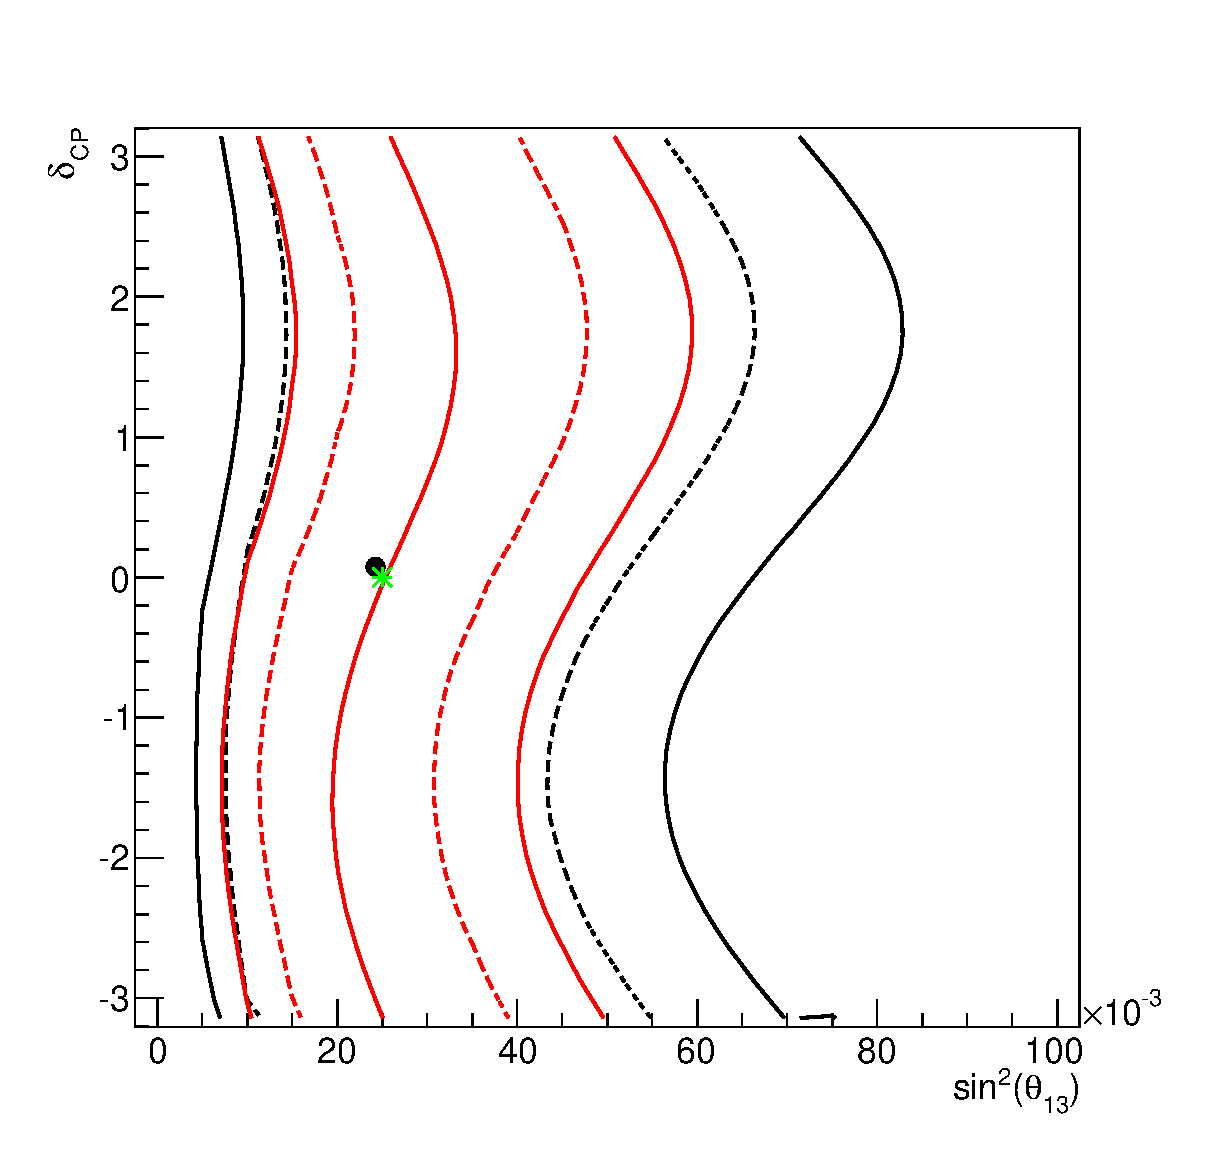
\includegraphics[width=15pc]{./images/appendix/fake_dataset_fits/fake_dataset7_chisq_theta13_deltacp_global_min_new.eps}
\caption {
  68\% and 90\% CL regions in ($sin^{2}\theta_{13}$, $\delta_{CP}$) space for fake dataset \#4.
  At each point, $\chi^2$ was minimized with respect to 
  $|\Delta m^{2}|$, $\sin^{2}\theta_{23}$
  and all relevant nuisance parameters for the joint analysis (black)
  and with respect to all relevant nuisance parameters for the appearance analysis (red).
  Notice that different methods are used to
  construct confidence regions for the joint analysis (global minimum) and for the 
  stand-alone appearance analysis (raster scan).
}
\label{fig:toymc4_confreg_sinsqtheta13_deltacp}
\end{minipage}
\hspace{0.03\linewidth}
\begin{minipage}[t]{0.48\linewidth}
\center
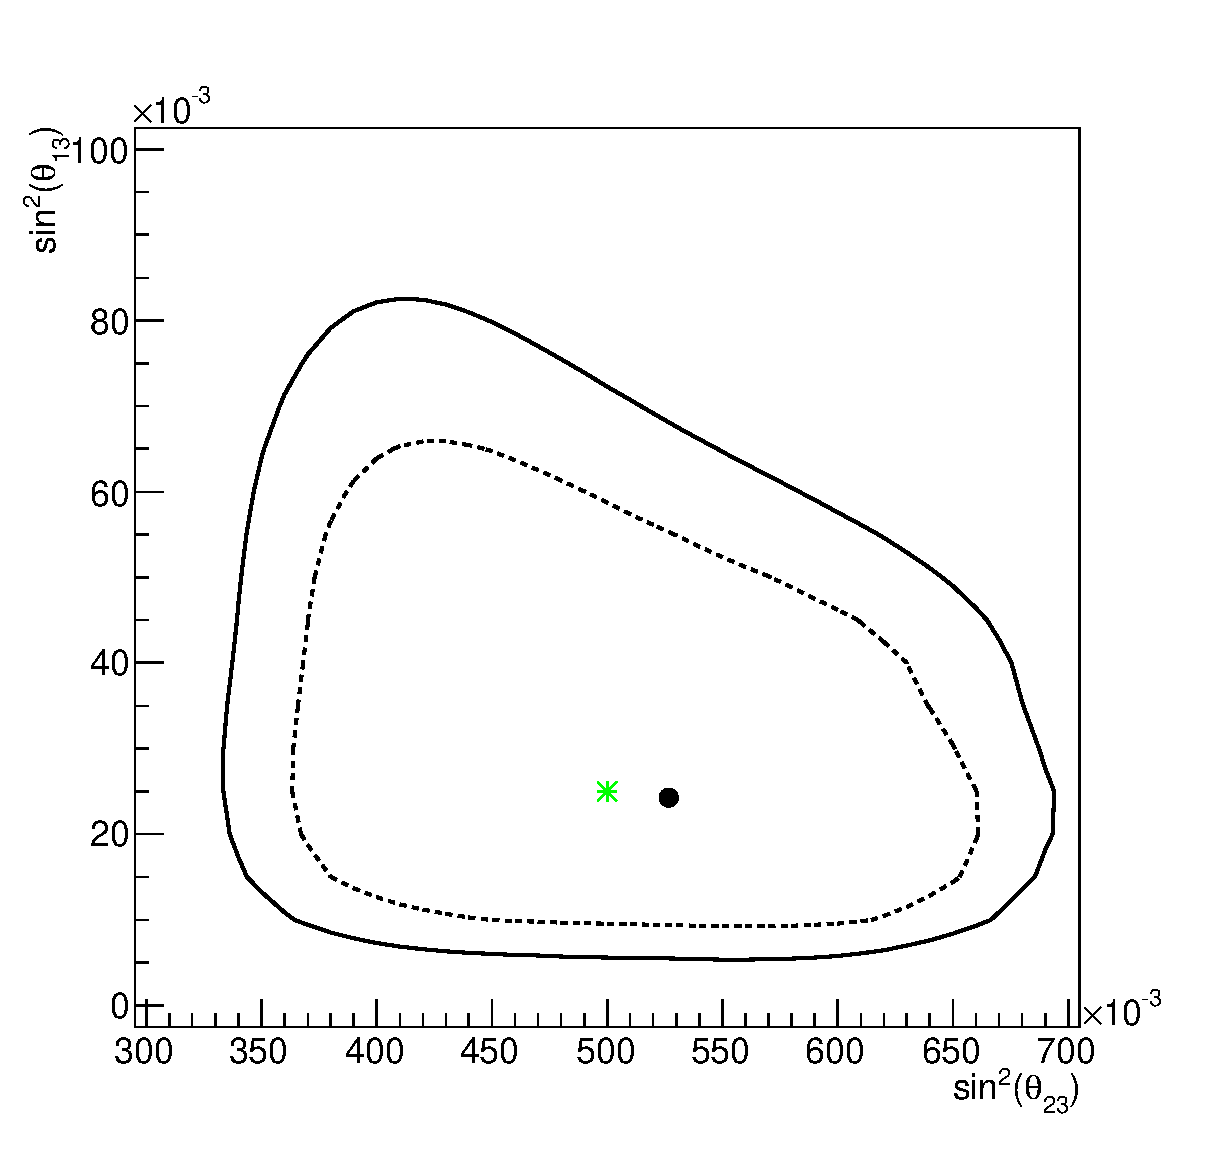
\includegraphics[width=15pc]{./images/appendix/fake_dataset_fits/fake_dataset7_chisq_theta13_theta23_global_min_new.eps}
\caption {
  68\% and 90\% CL regions in ($sin^{2}\theta_{23}$, $sin^{2}\theta_{13}$) space for fake dataset \#4.
  At each point, $\chi^2$ was minimized with respect to 
  all oscillation parameters not shown (and not considered to be fixed)
  and all relevant nuisance parameters.
}
\label{fig:toymc4_confreg_sinsqtheta23_sinsqtheta13}
\end{minipage}

\end{figure*}

% 
% 
% ..............................................
% Fake dataset #5 
% 
%

\clearpage

%
% delta\chisq and contours
%

\begin{figure*}[htb]

\begin{minipage}[t]{0.22\linewidth}
\center
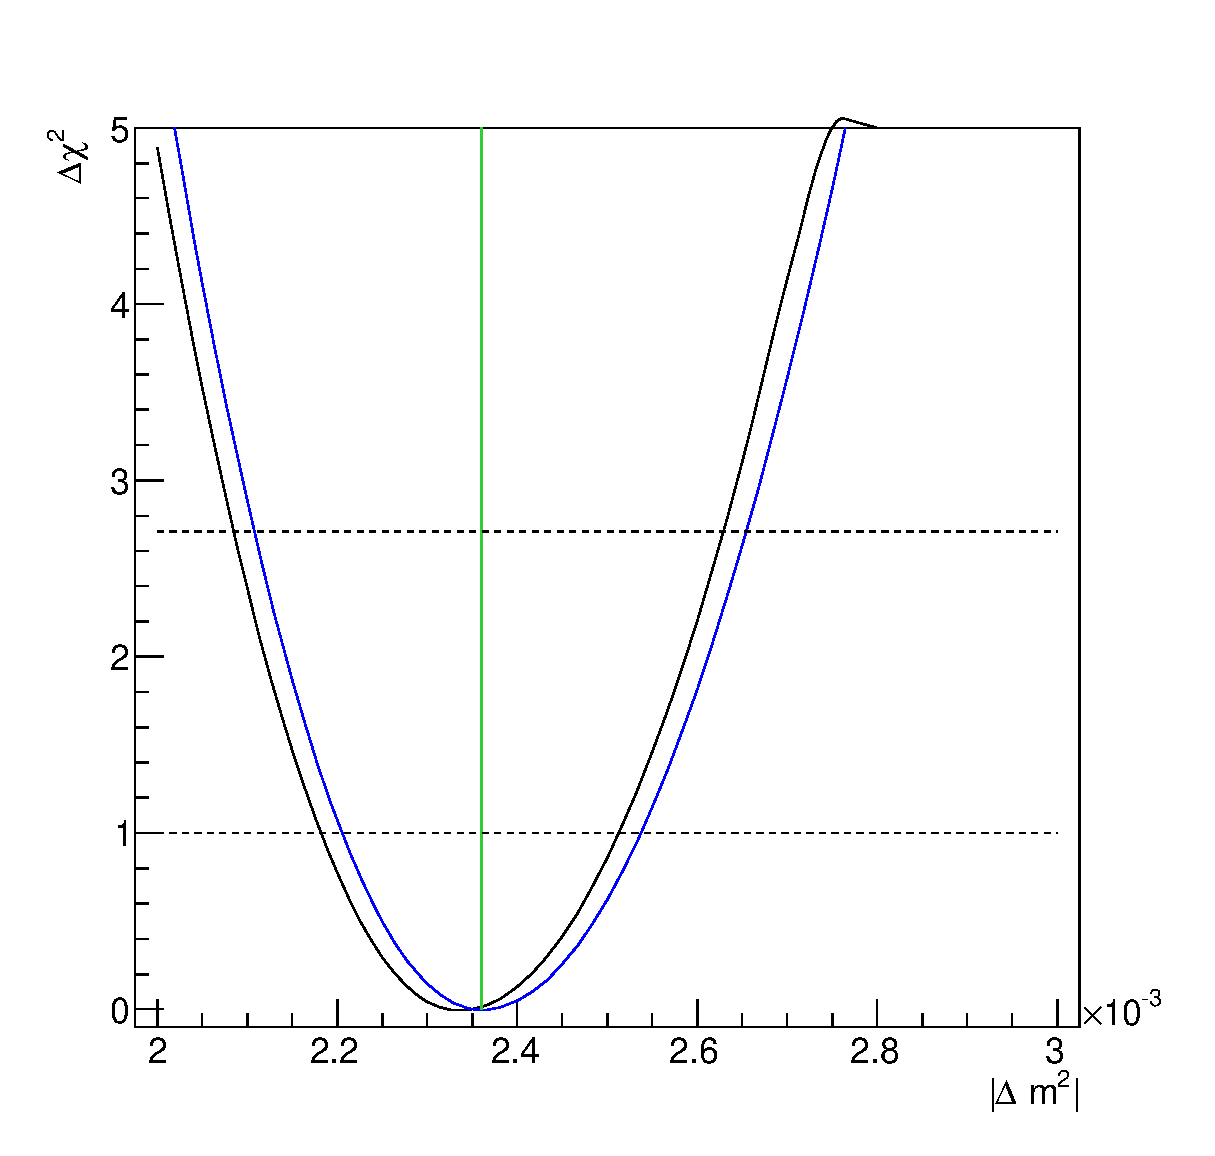
\includegraphics[width=9pc]{./images/appendix/fake_dataset_fits/fake_dataset9_chisq_dm23sq_global_min_new.eps}
\caption {
  $\Delta\chi^2$ as function of $|\Delta m^{2}|$ for fake dataset \#5.
  At each point, $\chi^2$ was minimized with respect to 
  $\sin^{2}\theta_{23}$, $\sin^{2}\theta_{13}$, $\delta_{CP}$
  and all relevant nuisance parameters for the joint analysis (black)
  and with respect to $\sin^{2}\theta_{23}$ and all relevant nuisance
  parameters for the disappearance analysis (blue).
}
\label{fig:toymc5_dchisq_Dmsq}
\end{minipage}
\hspace{0.02\linewidth}
\begin{minipage}[t]{0.22\linewidth}
\center
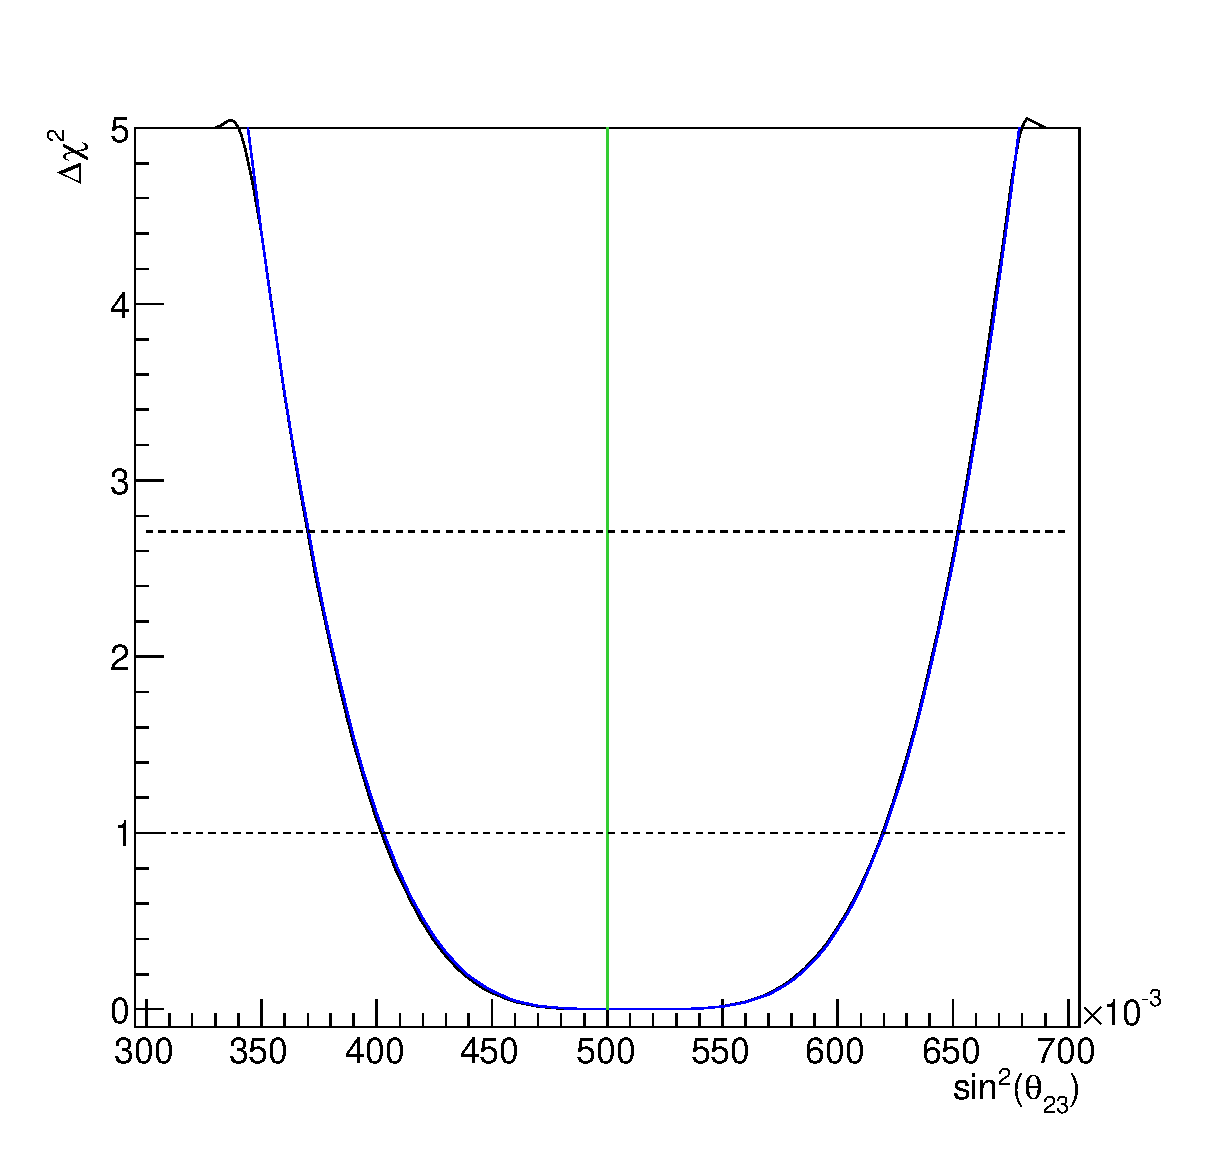
\includegraphics[width=9pc]{./images/appendix/fake_dataset_fits/fake_dataset9_chisq_theta23_global_min_new.eps}
\caption {
  $\Delta\chi^2$ as function of $sin^{2}\theta_{23}$ for fake dataset \#5.
  At each point, $\chi^2$ was minimized with respect to 
  $|\Delta m^{2}|$, $\sin^{2}\theta_{13}$, $\delta_{CP}$
  and all relevant nuisance parameters for the joint analysis (black)
  and with respect to $\sin^{2}\theta_{23}$ and all relevant nuisance
  parameters for the disappearance analysis (blue).
}
\label{fig:toymc5_dchisq_sinsqtheta23}
\end{minipage}
\hspace{0.02\linewidth}
\begin{minipage}[t]{0.22\linewidth}
\center
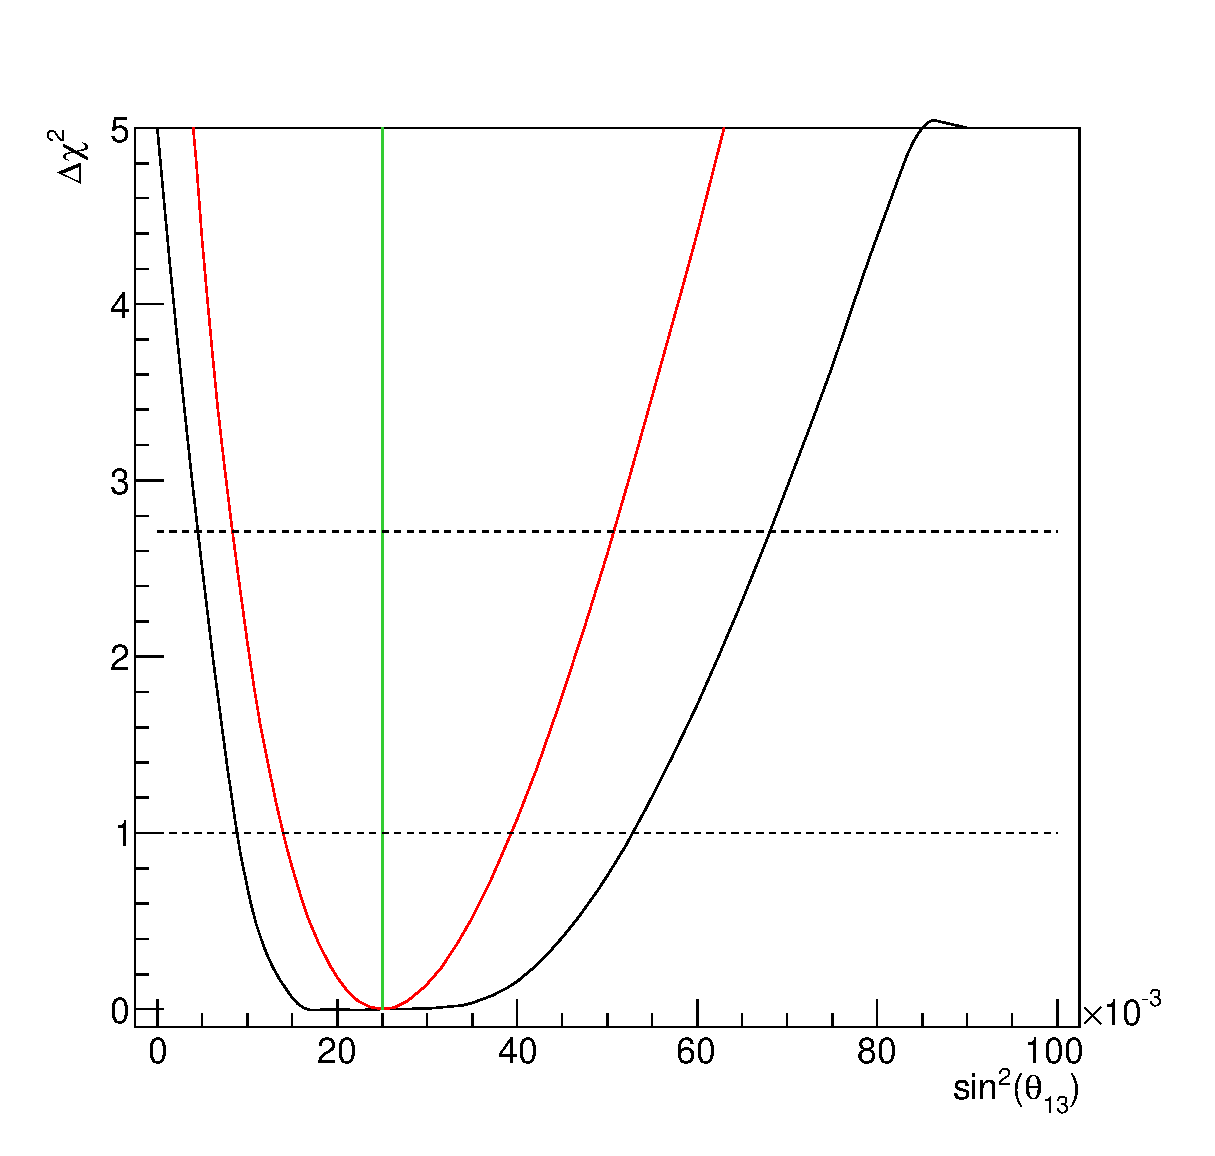
\includegraphics[width=9pc]{./images/appendix/fake_dataset_fits/fake_dataset9_chisq_theta13_global_min_new.eps}
\caption {
  $\Delta\chi^2$ as function of $sin^{2}\theta_{13}$ for fake dataset \#5.
  At each point, $\chi^2$ was minimized with respect to 
  $\sin^{2}\theta_{23}$, $\sin^{2}\theta_{13}$, $\delta_{CP}$
  and all relevant nuisance parameters for the joint analysis (black)
  and with respect to all relevant nuisance parameters 
  ($\delta_{CP}$ is fixed to 0) for the appearance analysis (red).
}
\label{fig:toymc5_dchisq_sinsqtheta13}
\end{minipage}
\hspace{0.02\linewidth}
\begin{minipage}[t]{0.22\linewidth}
\center
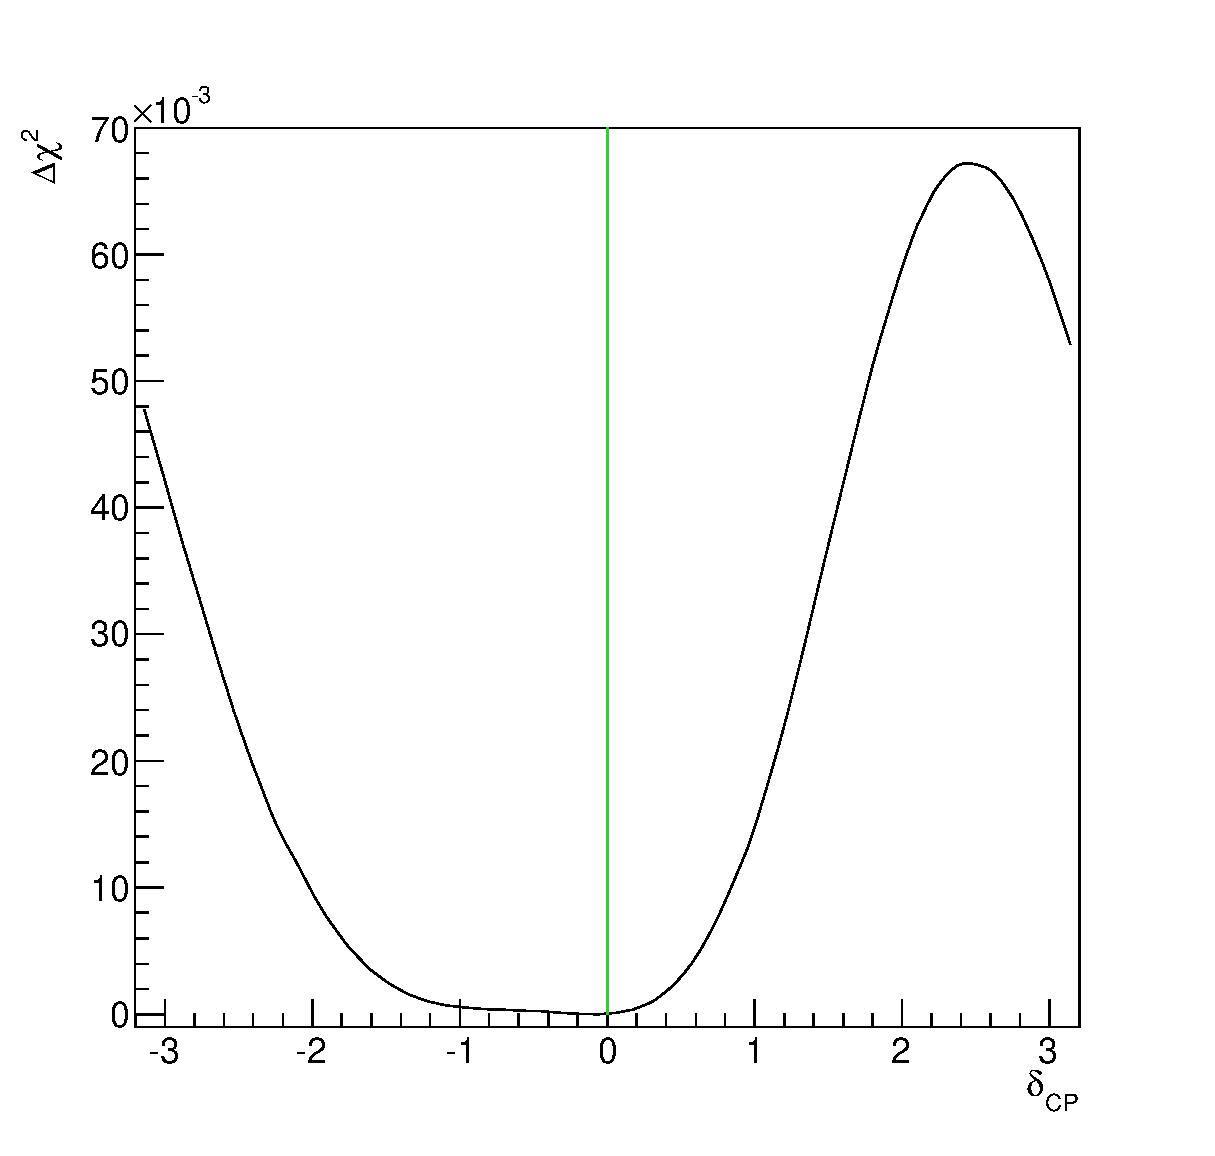
\includegraphics[width=9pc]{.//images/appendix/fake_dataset_fits/fake_dataset9_chisq_deltacp_global_min_new.eps}
\caption {
  $\Delta\chi^2$ as function of $\delta_{CP}$ for fake dataset \#5.
  At each point, $\chi^2$ was minimized with respect to 
  all oscillation parameters not shown (and not considered to be fixed)
  and all relevant nuisance parameters.
}
\label{fig:toymc5_dchisq_deltacp}
\end{minipage}
\vfill
\vspace*{0.7cm}
\begin{minipage}[t]{0.48\linewidth}
\center
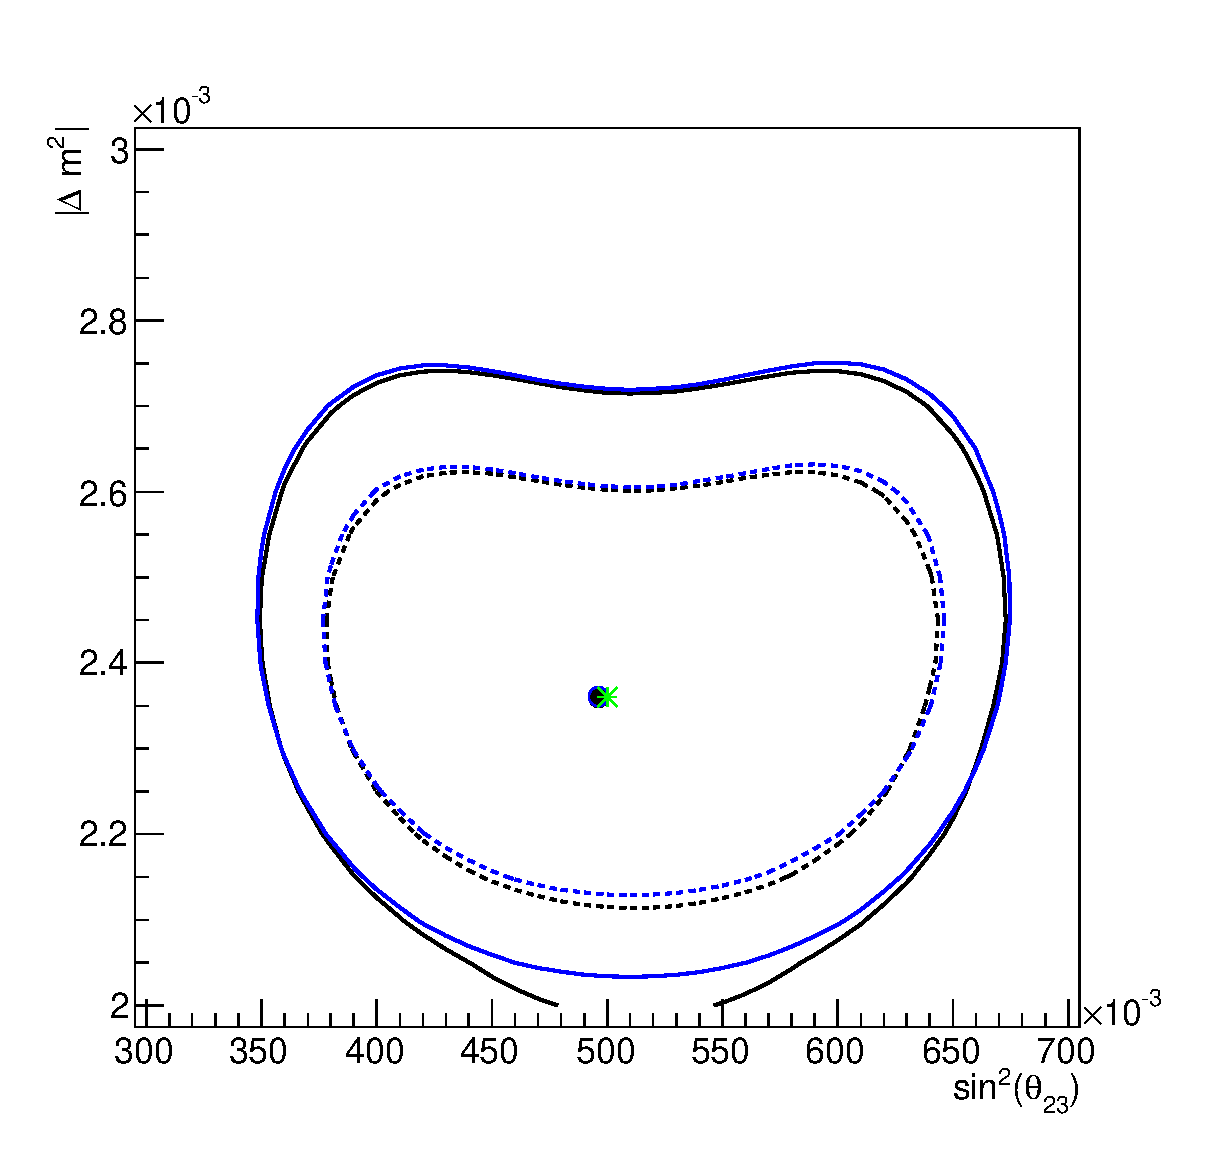
\includegraphics[width=15pc]{./images/appendix/fake_dataset_fits/fake_dataset9_chisq_theta23_dm23sq_global_min_new.eps}
\caption {
  68\% and 90\% CL regions in ($sin^{2}\theta_{23}$, $|\Delta m^{2}|$) space for fake dataset \#5.
  At each point, $\chi^2$ was minimized with respect to 
  $\sin^{2}\theta_{13}$, $\delta_{CP}$
  and all relevant nuisance parameters for the joint analysis (black)
  and with respect to all relevant nuisance parameters for the disappearance analysis (blue).
}
\label{fig:toymc5_confreg_sinsqtheta23_Dmsq}
\end{minipage}
\hspace{0.03\linewidth}
\begin{minipage}[t]{0.48\linewidth}
\center
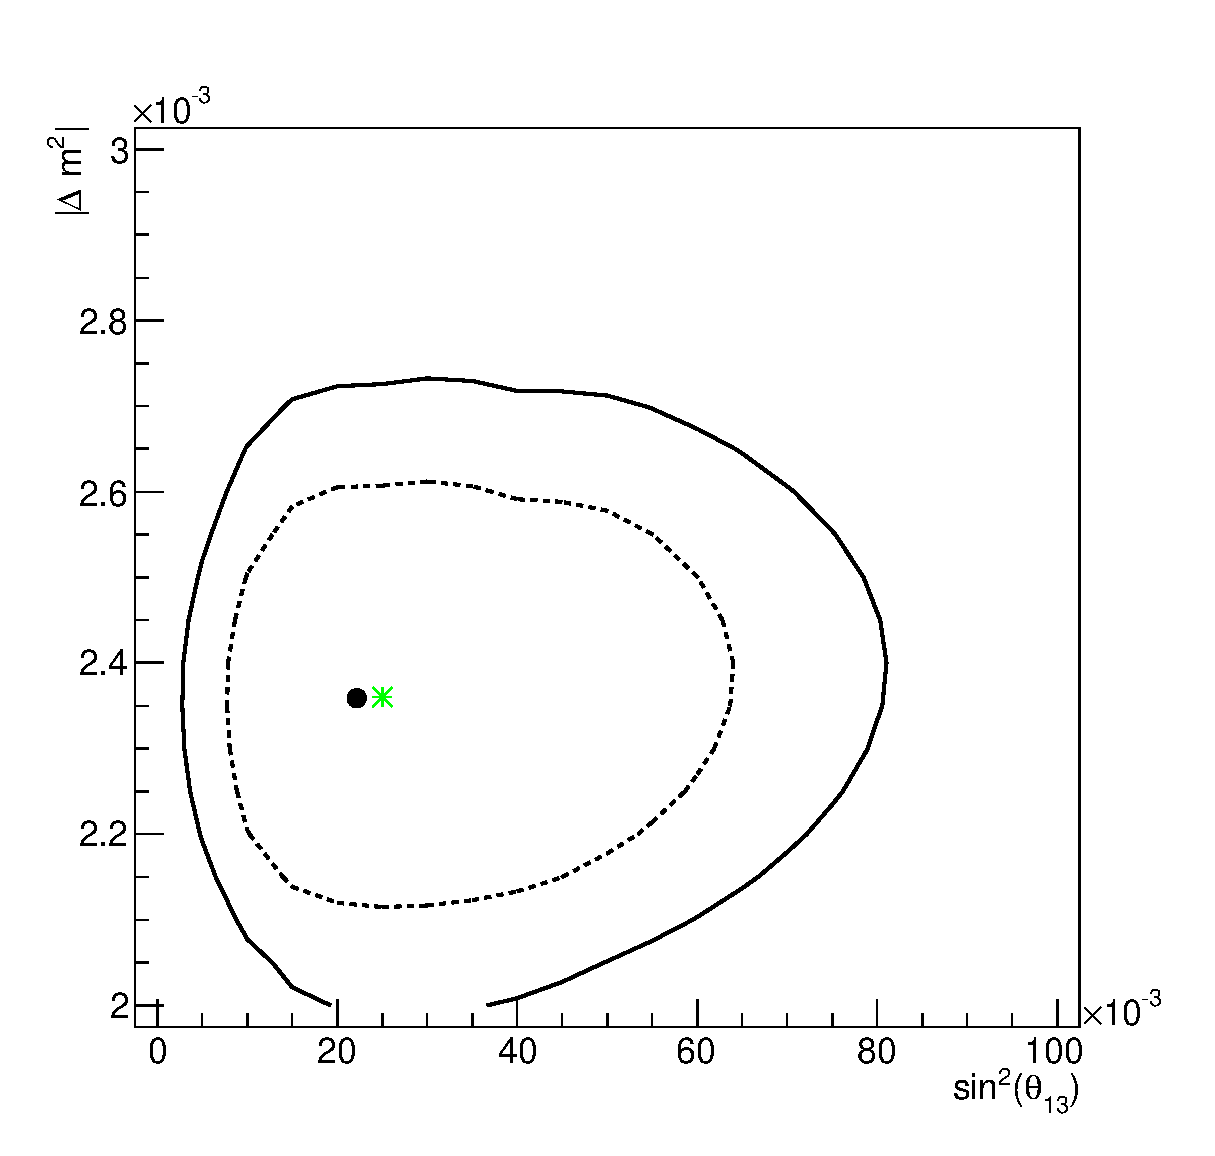
\includegraphics[width=15pc]{./images/appendix/fake_dataset_fits/fake_dataset9_chisq_theta13_dm23sq_global_min_new.eps}
\caption {
  68\% and 90\% CL regions in ($sin^{2}\theta_{13}$, $|\Delta m^{2}|$) space for fake dataset \#5.
  At each point, $\chi^2$ was minimized with respect to 
  all oscillation parameters not shown (and not considered to be fixed)
  and all relevant nuisance parameters.
}
\label{fig:toymc5_confreg_sinsqtheta13_Dmsq}
\end{minipage}

\vfill
\vspace*{0.7cm}

\begin{minipage}[t]{0.48\linewidth}
\center
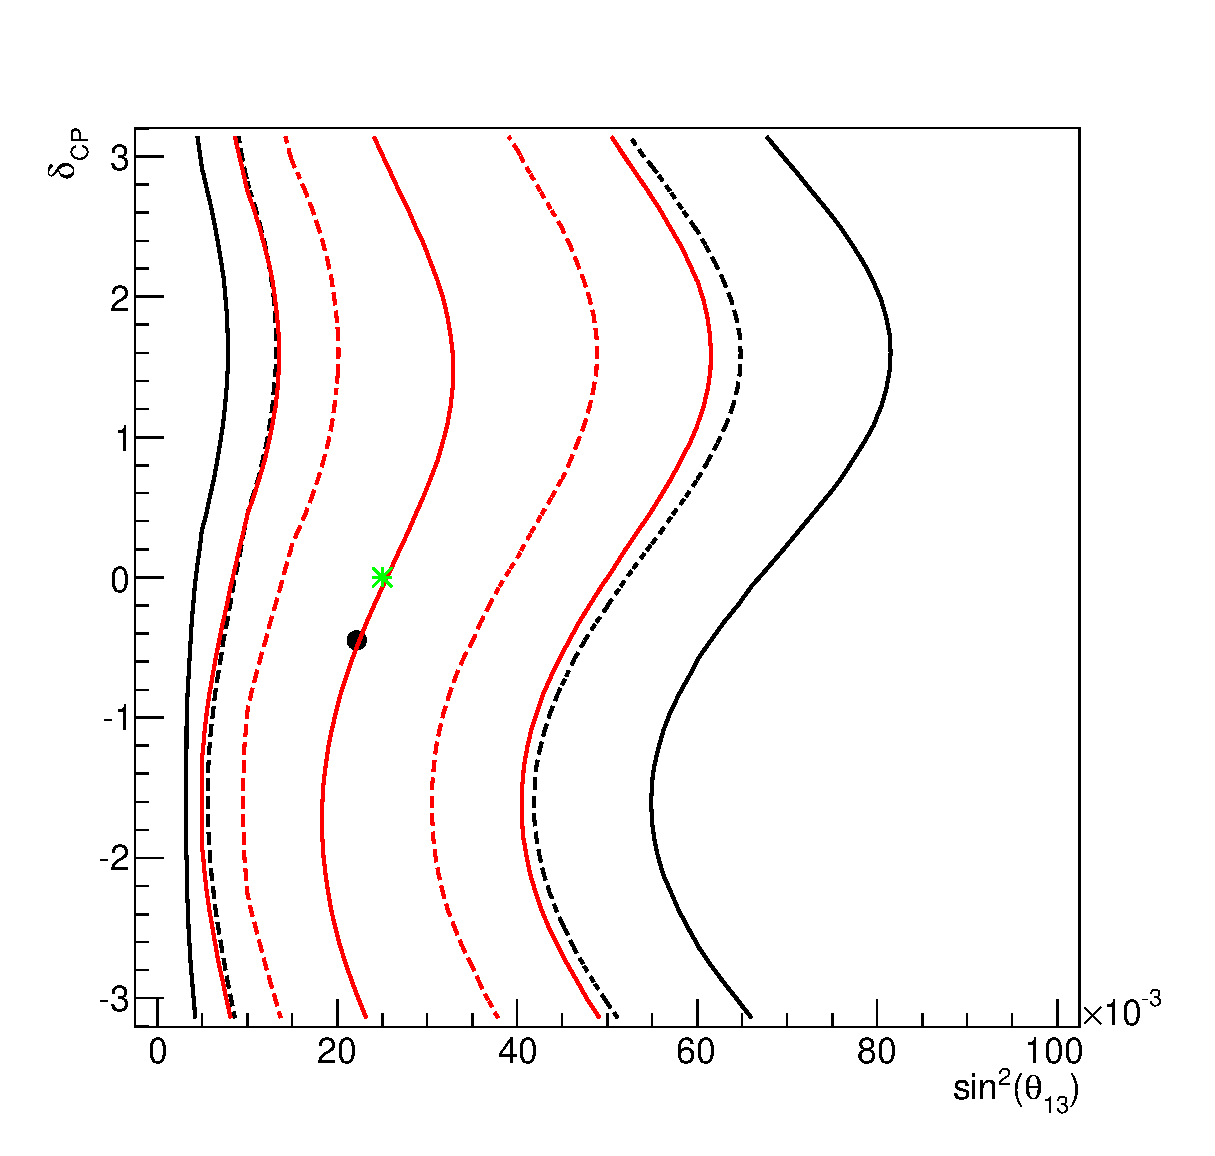
\includegraphics[width=15pc]{./images/appendix/fake_dataset_fits/fake_dataset9_chisq_theta13_deltacp_global_min_new.eps}
\caption {
  68\% and 90\% CL regions in ($sin^{2}\theta_{13}$, $\delta_{CP}$) space for fake dataset \#5.
  At each point, $\chi^2$ was minimized with respect to 
  $|\Delta m^{2}|$, $\sin^{2}\theta_{23}$
  and all relevant nuisance parameters for the joint analysis (black)
  and with respect to all relevant nuisance parameters for the appearance analysis (red).
  Notice that different methods are used to
  construct confidence regions for the joint analysis (global minimum) and for the 
  stand-alone appearance analysis (raster scan).
}
\label{fig:toymc5_confreg_sinsqtheta13_deltacp}
\end{minipage}
\hspace{0.03\linewidth}
\begin{minipage}[t]{0.48\linewidth}
\center
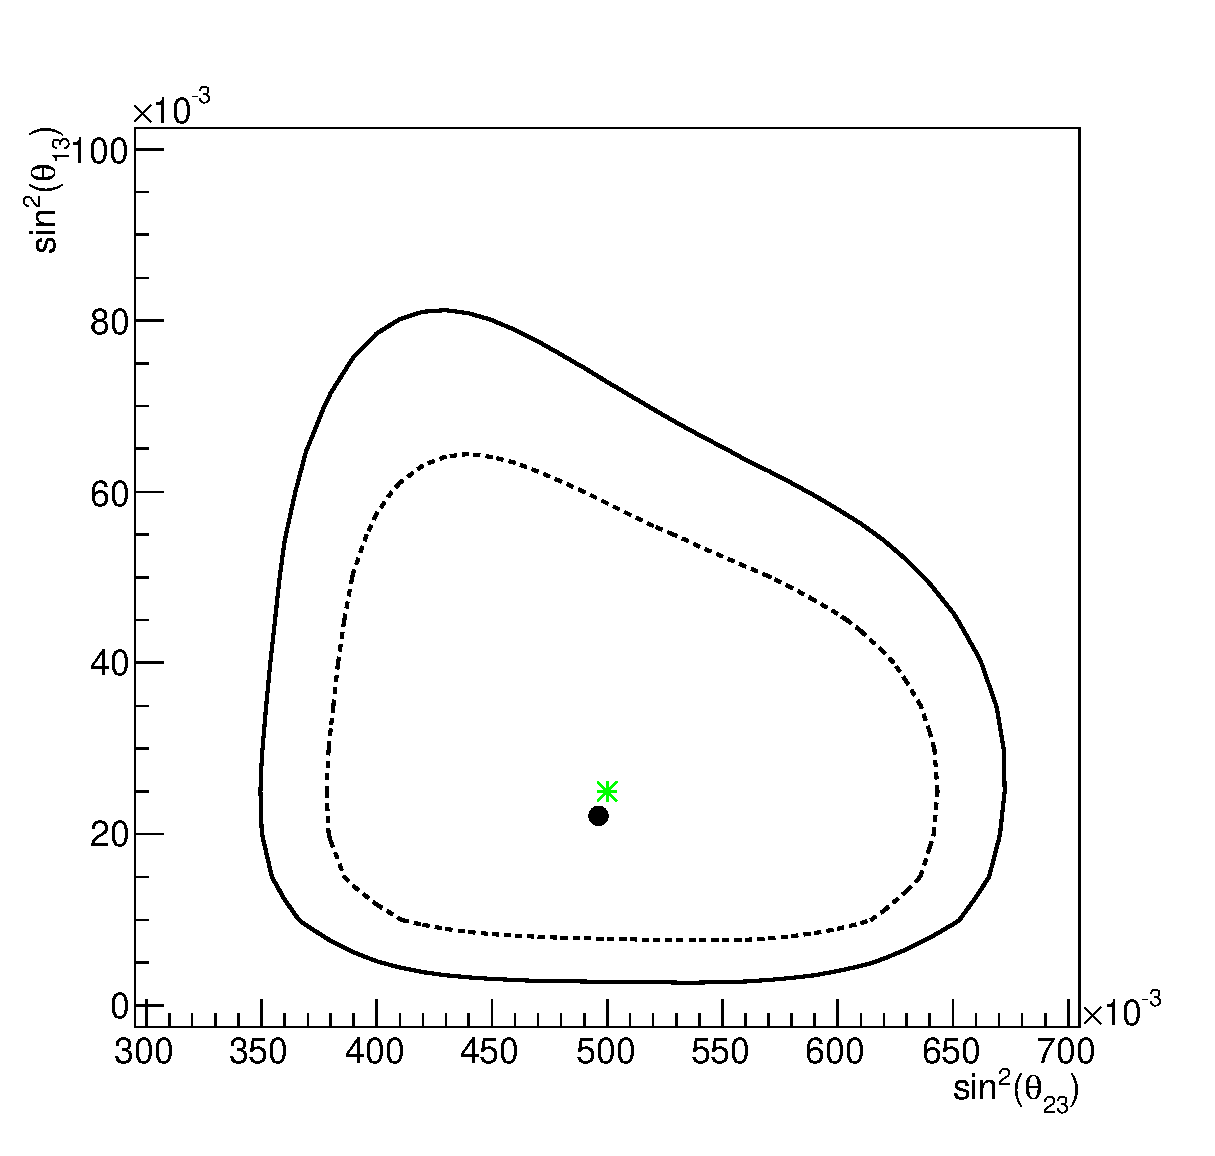
\includegraphics[width=15pc]{./images/appendix/fake_dataset_fits/fake_dataset9_chisq_theta13_theta23_global_min_new.eps}
\caption {
  68\% and 90\% CL regions in ($sin^{2}\theta_{23}$, $sin^{2}\theta_{13}$) space for fake dataset \#5.
  At each point, $\chi^2$ was minimized with respect to 
  all oscillation parameters not shown (and not considered to be fixed)
  and all relevant nuisance parameters.
}
\label{fig:toymc5_confreg_sinsqtheta23_sinsqtheta13}
\end{minipage}

\end{figure*}


\clearpage


%%%%%%%%%%%%%%%%%%%%%%%%%%%%%%%%%%%%%%%%%%%%%%%%%%%%%%%%%%%%%%%%
%%%%%%%%%%%%%%%%%%%%%%%%%%%%%%%%%%%%%%%%%%%%%%%%%%%%%%%%%%%%%%%%
%%%%%%%%%%%% REALISTIC FAKE DATASETS %%%%%%%%%%%%%%%%%%%%%%%%%%%%%%%%%%%%%
%%%%%%%%%%%%%%%%%%%%%%%%%%%%%%%%%%%%%%%%%%%%%%%%%%%%%%%%%%%%%%%%



\begin{sidewaystable}[htb]
\small
\centering
\begin{tabular}{@{}|p{0.1cm}p{2.5cm}|p{1.5cm}p{1cm}p{1cm}p{1cm}|p{1cm}|p{1.0cm}p{1.0cm}|p{1.2cm}p{1.2cm}|p{1.5cm}|@{}}
\hline
Set &   & $|\Delta m^2|$  & sin$^2\theta_{23}$ & sin$^2\theta_{13}$  & $\delta_{CP}$  &  MH & N$_{SK}^{1R\mu}$ & N$_{SK}^{1Re}$ & $\chi^2$/ndf & p-value & Systematics \\
 &   & ( $\times$10$^{-3}$ eV$^{2}$/c$^{4}$) &  &   &  &   &  & &  & &  \\
\hline
6  & true                      & {\bf 2.36 }   & {\bf 0.5}   & {\bf 0.025}   & {\bf 0.0}  & {\bf Normal} & {\bf 63 }   & {\bf 7}    & --        & --   & {\bf Nominal} \\
   & fit (joint)               &    2.369       &  0.509     &   0.016    &   2.110 & (fixed)    &   60.887   &   6.752    &  81.85/94          & 0.95  & See Fig. \ref{fig:toymc6_1Rmu_bestfit_spectrum} -  \\
   & fit ($\nu_{e}$ app.)      & --                             & --         &   0.011    & 0(fixed)  &     & --         &     6.741  &    16.98/24     & 0.98 &  \ref{fig:toymc6_confreg_sinsqtheta23_sinsqtheta13} \\
   & fit ($\nu_{\mu}$ disapp.) &    2.356      &   0.514    & --         & --       &   &   61.010    & --          & 65.09/71    &  0.81 &   \\
\hline
7  & true                      & {\bf 2.36 }   & {\bf 0.5}   & {\bf 0.025}   & {\bf 0.0}  & {\bf Normal} & {\bf 55}   & {\bf 11}    & --          & --   & {\bf Random} \\
   & fit (joint)               &     2.511      &    0.516   &    0.030   &   0.722 & (fixed)    &    54.802  &     10.962  & 73.86/94        & 0.35  & See Fig. \ref{fig:toymc7_1Rmu_bestfit_spectrum} -  \\
   & fit ($\nu_{e}$ app.)      & --                             & --         &    0.026   & 0(fixed)  &     & --         &   10.894    & 22.70/24      & 0.20 &   \ref{fig:toymc7_confreg_sinsqtheta23_sinsqtheta13}\\
   & fit ($\nu_{\mu}$ disapp.) &   2.492       &     0.514  & --         & --       &    &55.406       & --          & 52.24/71    &  0.53  &   \\
   \hline
8  & true                      & {\bf 2.36 }   & {\bf 0.5}   & {\bf 0.025}   & {\bf 0.0}  & {\bf Normal} & {\bf 55}   & {\bf 12}    & --          & --   & {\bf $E_{reco}$ scale: -1$\sigma$} \\
   & fit (joint)               &    2.431       &  0.520     &     0.036  &   0.707 & (fixed)    &    56.166  &  12.679     & 74.34/94        & 0.17  & See Fig. \ref{fig:toymc8_1Rmu_bestfit_spectrum} -  \\
   & fit ($\nu_{e}$ app.)      & --                             & --         &   0.032    & 0(fixed)  &     & --         &  12.695     & 16.65/24      & 0.39 &   \ref{fig:toymc8_confreg_sinsqtheta23_sinsqtheta13}\\
   & fit ($\nu_{\mu}$ disapp.) &     2.431     &    0.514   & --         & --       &    &  56.821     & --          & 58.10/71    & 0.09 &   \\
\hline
9  & true                      & {\bf 2.36 }   & {\bf 0.38}   & {\bf 0.025}   & {\bf 0.0}  & {\bf Normal} & {\bf 53}   & {\bf 11}    & --          & --   & {\bf Nominal} \\
   & fit (joint)               &     2.317      &    0.400   &    0.030   &   -0.263 & (fixed)    &    61.157  &     11.138  & 101.18/94        & 0.73  & See Fig. \ref{fig:toymc9_1Rmu_bestfit_spectrum} -  \\
   & fit ($\nu_{e}$ app.)      & --                             & --         &    0.026   & 0(fixed)  &     & --         &   11.272    & 29.70/24      & 0.71 &   \ref{fig:toymc9_confreg_sinsqtheta23_sinsqtheta13}\\
   & fit ($\nu_{\mu}$ disapp.) &   2.278       &     0.403  & --         & --       &    & 60.964       & --          & 72.07/71    & 0.49 &   \\
   \hline
10  & true                      & {\bf 2.36 }   & {\bf 0.5}   & {\bf 0.015}   & {\bf 0.0}  & {\bf Normal} & {\bf 57}   & {\bf 5}    & --          & --   & {\bf Nominal} \\
   & fit (joint)               &     2.427      &    0.505   &    0.009   &   1.072 & (fixed)    &    56.061  &     5.087  & 78.51/94        & 0.30  & See Fig. \ref{fig:toymc10_1Rmu_bestfit_spectrum} -  \\
   & fit ($\nu_{e}$ app.)      & --                             & --         &    0.006   & 0(fixed)  &     & --         &   5.047    & 17.13/24      & 0.43 &   \ref{fig:toymc10_confreg_sinsqtheta23_sinsqtheta13}\\
   & fit ($\nu_{\mu}$ disapp.) &   2.420       &     0.514  & --         & --       &    & 56.235       & --          & 62.16/71    & 0.27 &   \\
   \hline
11  & true                      & {\bf 2.36 }   & {\bf 0.5}   & {\bf 0.025}   & {\bf -$\pi/2$}  & {\bf Normal} & {\bf 69}   & {\bf 13}    & --          & --   & {\bf Nominal} \\
   & fit (joint)               &     2.455      &    0.389   &    0.048   &   0.706 & (fixed)    &    68.012  &     12.594  & 75.27/94        & 0.25 & See Fig. \ref{fig:toymc11_1Rmu_bestfit_spectrum} -  \\
   & fit ($\nu_{e}$ app.)      & --                             & --         &    0.031   & 0(fixed)  &     & --         &   12.541    & 24.58/24      & 0.08 &   \ref{fig:toymc11_confreg_sinsqtheta23_sinsqtheta13}\\
   & fit ($\nu_{\mu}$ disapp.) &   2.411       &     0.384  & --         & --       &    & 68.452       & --          & 50.88/71    & 0.80 &   \\
   \hline
12  & true                      & {\bf 2.2 }   & {\bf 0.5}   & {\bf 0.025}   & {\bf 0.0}  & {\bf Normal} & {\bf 53}   & {\bf 7}    & --          & --   & {\bf Nominal} \\
   & fit (joint)               &     2.234      &    0.506   &    0.013   &   3.141 & (fixed)    &    57.620  &     6.972  & 90.38/94        & 0.93  & See Fig. \ref{fig:toymc12_1Rmu_bestfit_spectrum} -  \\
   & fit ($\nu_{e}$ app.)      & --                             & --         &    0.012   & 0(fixed)  &     & --         &   6.961    & 18.67/24      & 0.85 &   \ref{fig:toymc12_confreg_sinsqtheta23_sinsqtheta13}\\
   & fit ($\nu_{\mu}$ disapp.) &   2.220       &     0.513  & --         & --       &    & 57.665       & --          & 72.36/71    & 0.76 &   \\
     \hline
13  & true                      & {\bf 2.36 }   & {\bf 0.5}   & {\bf 0.025}   & {\bf 0.0}  & {\bf Inverted} & {\bf 52}   & {\bf 11}    & --          & --   & {\bf Nominal} \\
   & fit (joint)               &     2.503      &    0.513   &    0.029   &   -0.379  & (fixed)    &    54.485  &     11.374  & 73.72/94        & 0.58  & See Fig. \ref{fig:toymc13_1Rmu_bestfit_spectrum} -  \\
   & fit ($\nu_{e}$ app.)      & --                             & --         &    0.033   & 0(fixed)  &     & --         &   11.450    & 15.82/24      & 0.60 &   \ref{fig:toymc13_confreg_sinsqtheta23_sinsqtheta13}\\
   & fit ($\nu_{\mu}$ disapp.) &   2.513       &     0.511  & --         & --       &    & 54.708       & --          & 58.09/71    & 0.53 &   \\


\hline
\end{tabular}
\caption{
  True input values (shown in bold) and VALOR best-fit values for a test ensemble of 7 fake datasets with statistical fluctuations
}
\label{tab:toymc_fits:best_fit_values_realistic}
\end{sidewaystable}

\clearpage
% 
% 
% ..............................................
% Fake dataset #6 
% 
%

%
% best-fit spectra and pulls
%

\begin{figure*}[htb]

\begin{minipage}[t]{0.46\linewidth}
\center
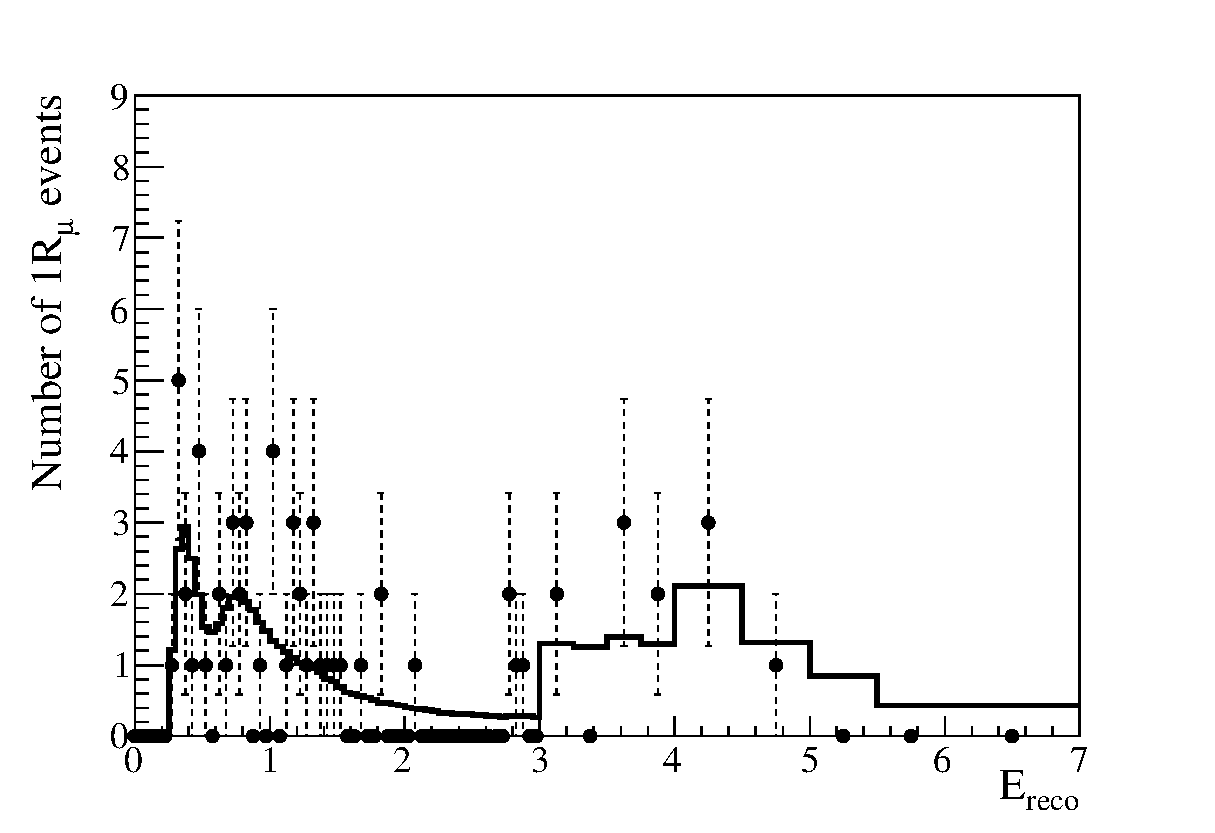
\includegraphics[width=15pc]{./images/appendix/fake_dataset_fits/realistic_fake_dataset0_nh_1st_1Rmu.eps}
\caption {
  Single $\mu$-like ring event best-fit reconstructed energy spectrum
  to fake dataset \#6.
}
\label{fig:toymc6_1Rmu_bestfit_spectrum}
\end{minipage}
\hspace{0.03\linewidth}
\begin{minipage}[t]{0.46\linewidth}
\center
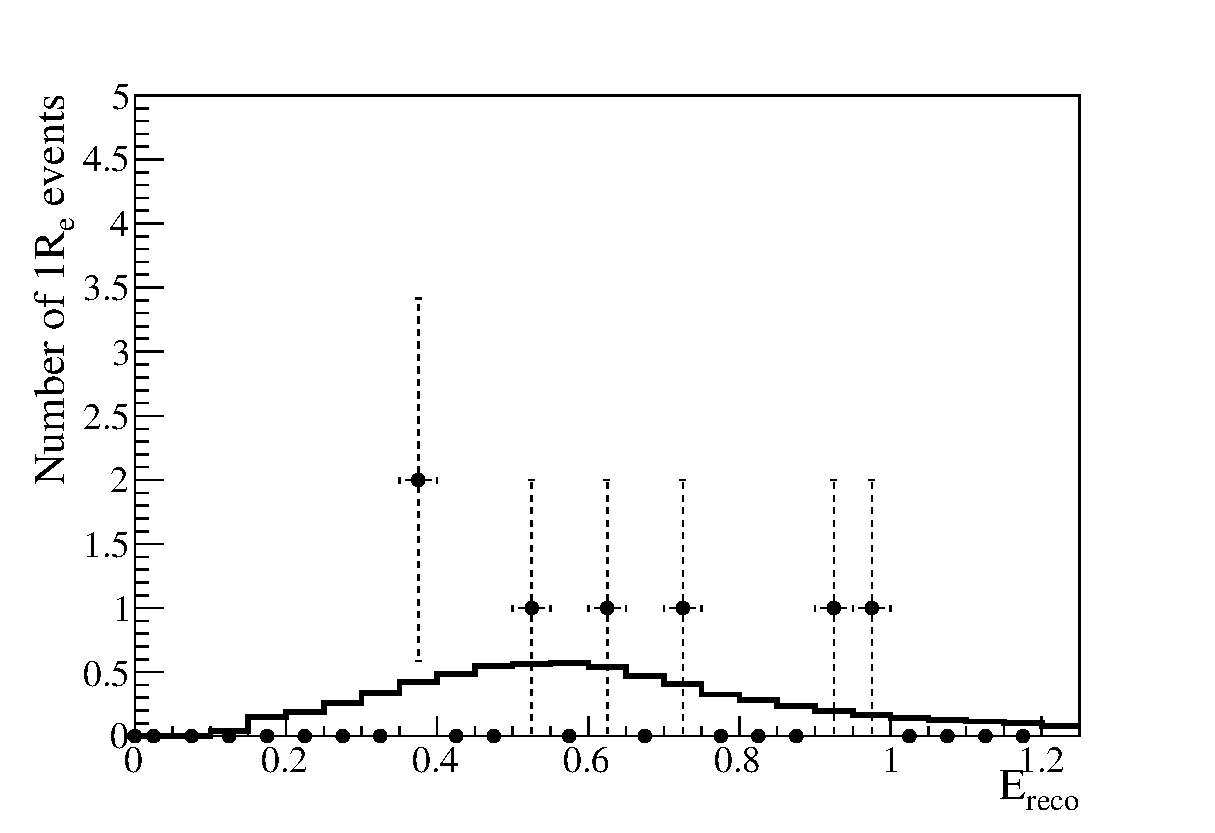
\includegraphics[width=15pc]{./images/appendix/fake_dataset_fits/realistic_fake_dataset0_nh_1st_1Re.eps}
\caption {
  Single e-like ring event best-fit reconstructed energy spectrum
  to fake dataset \#6.
}
\label{fig:toymc6_1Re_bestfit_spectrum}
\end{minipage}

\vfill
\vspace*{0.7cm}

\begin{minipage}[t]{0.90\linewidth}
\center
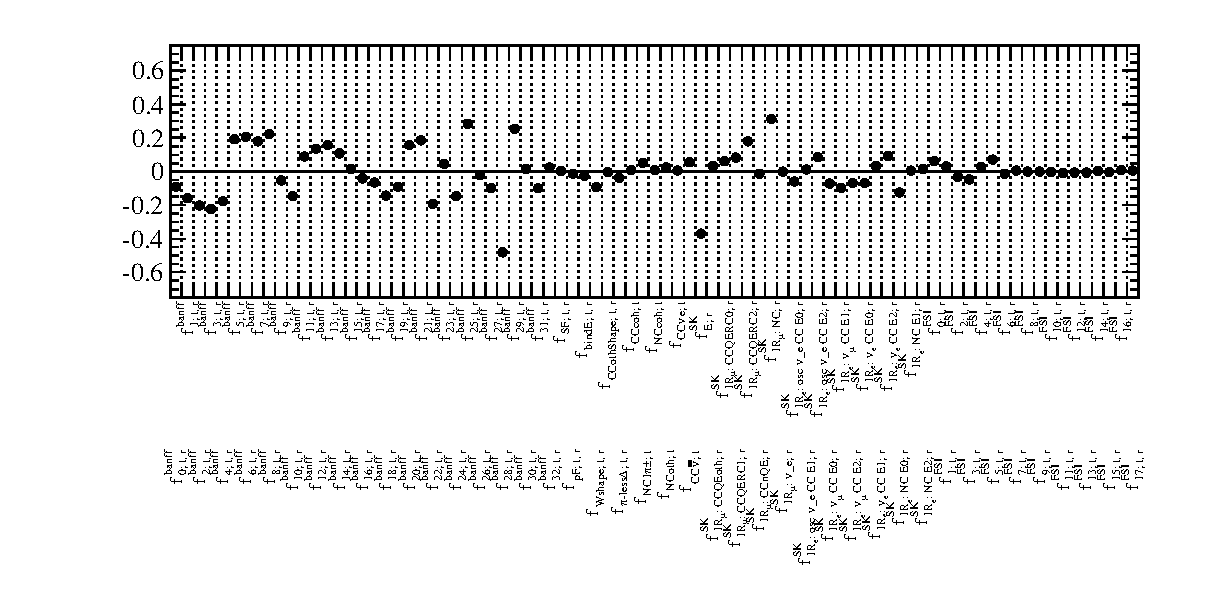
\includegraphics[width=30pc,angle=270]{./images/appendix/fake_dataset_fits/pulls_realistic_fake_dataset0_nh_1st.eps}
\caption {
  Systematic parameter pulls for the oscillation fit to fake dataset \#6.
}
\label{fig:toymc6_pulls}
\end{minipage}

\end{figure*}

\clearpage


%...........................................................
%
% chisq distributions used for calculating the fit p-values
%

\begin{figure*}[htb]

\begin{minipage}[t]{0.90\linewidth}
\center
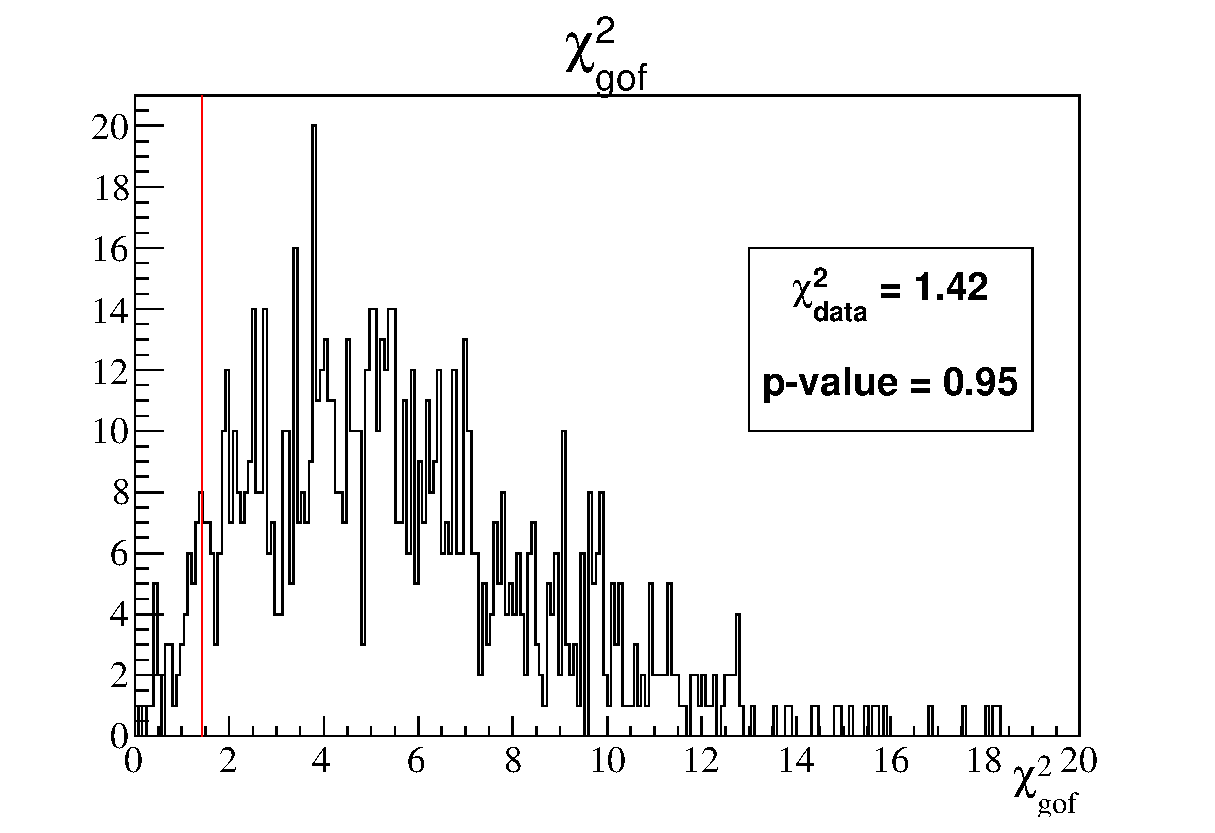
\includegraphics[width=30pc]{./images/appendix/fake_dataset_fits/realistic_fake_dataset0_nh_1st_gof_new.eps}
\caption {
  Distribution of $\chi^2_{gof}$, the goodness-of-fit (gof) $\chi^2$, 
  from 1k toy MC experiments generated at dataset \#6 joint 3-flavour analysis best-fit oscillation point.
  The $\chi^2_{gof}$ value for the dataset \#6 ($\chi^2_{data}$) is highlighted.
  All $\chi^2_{gof}$ values were computed 
  using the 5 (single $\mu$-like ring) + 1 (single e-like ring) 
  reconstructed energy binning scheme described in Sec.\ \ref{sec:goodness_of_fit},
}
\label{fig:toymc6_gofchisq}
\end{minipage}

\vfill
\vspace*{0.7cm}

\begin{minipage}[t]{0.46\linewidth}
\center
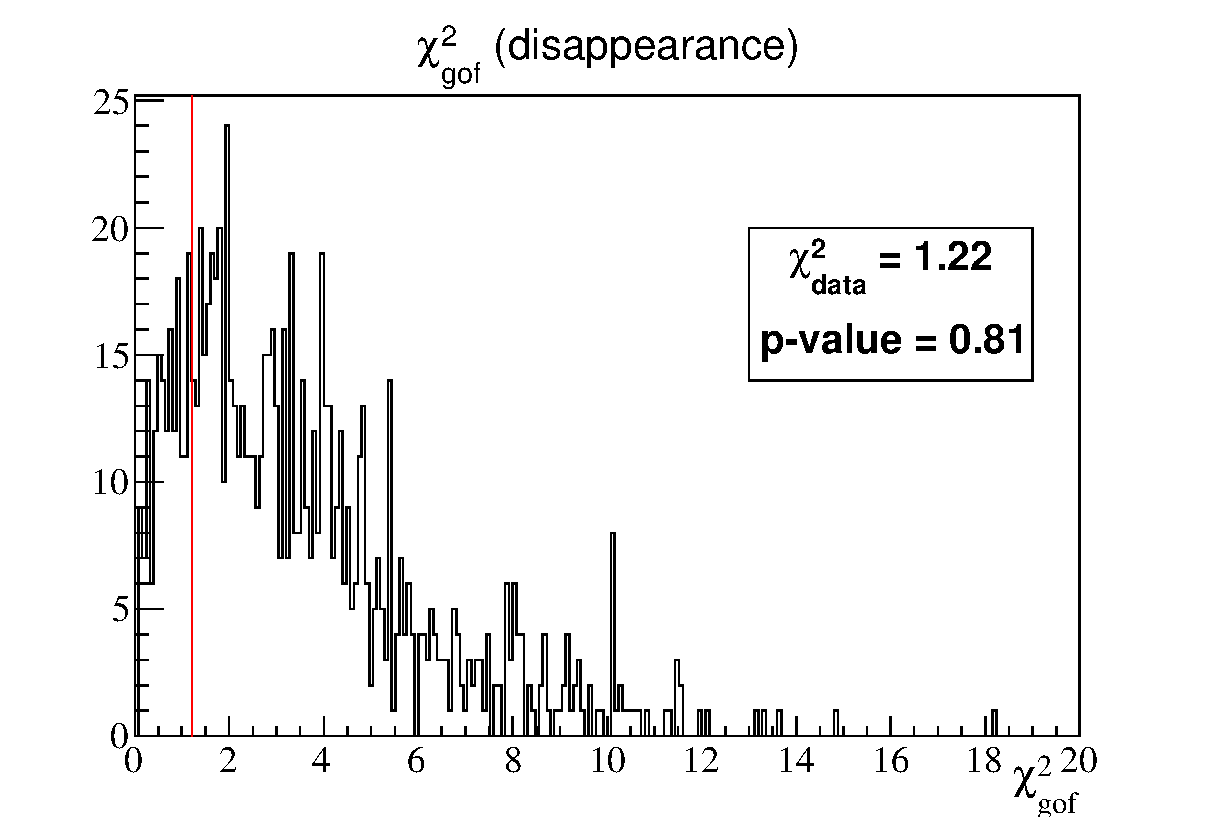
\includegraphics[width=18pc]{./images/appendix/fake_dataset_fits/realistic_fake_dataset0_nh_1st_gof_disap_new.eps}
\caption {
  Distribution of $\chi^2_{gof}$
  from 1k toy MC experiments generated at the dataset \#6 stand-alone 3-flavour $\nu_{\mu}$ disappearance analysis best-fit oscillation point.
  The $\chi^2_{gof}$ value for the dataset \#6 ($\chi^2_{data}$) is highlighted.
  All $\chi^2_{gof}$ values were computed 
  using the 5 (single $\mu$-like ring) 
  reconstructed energy binning scheme described in Sec.\ \ref{sec:goodness_of_fit},
}
\label{fig:toymc6_gofchisq_disapp}
\end{minipage}
\hspace{0.03\linewidth}
\begin{minipage}[t]{0.46\linewidth}
\center
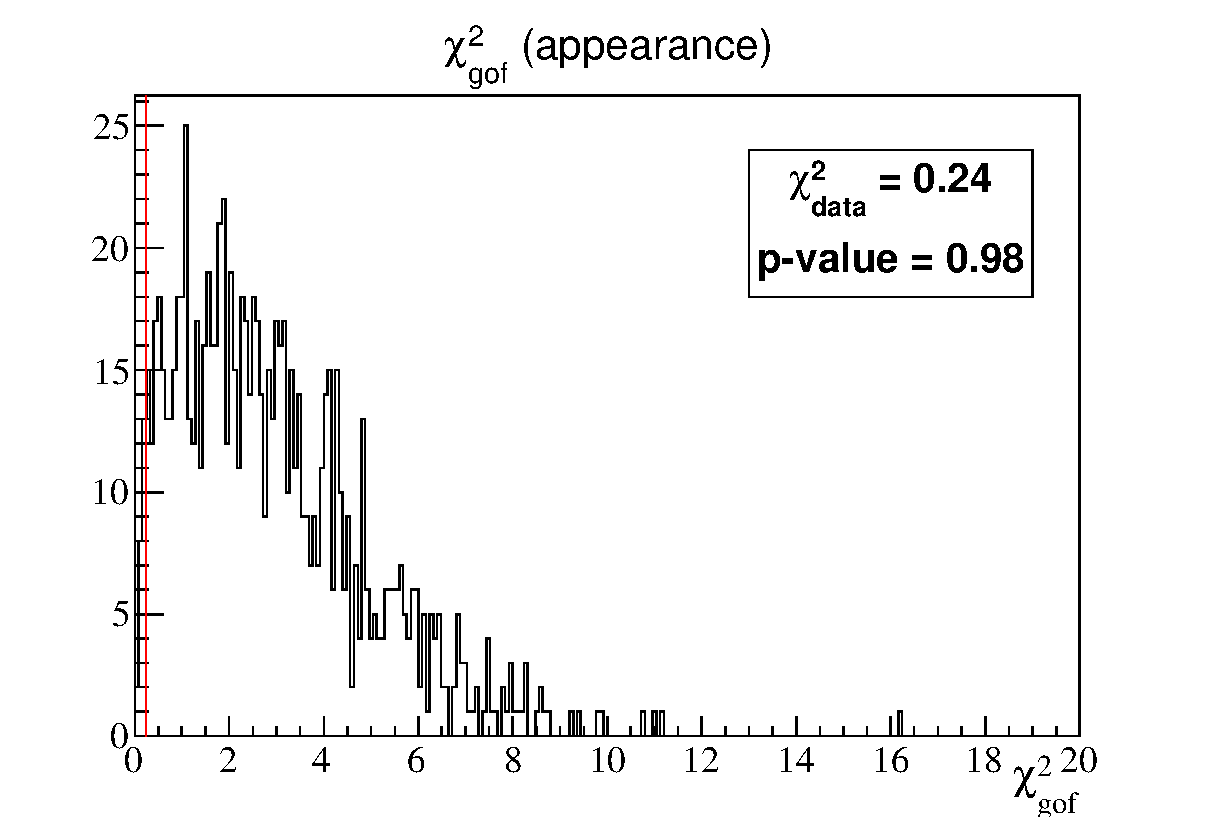
\includegraphics[width=18pc]{./images/appendix/fake_dataset_fits/realistic_fake_dataset0_nh_1st_gof_app_new.eps}
\caption {
  Distribution of $\chi^2_{gof}$
  from 1k toy MC experiments generated at the dataset \#6 stand-alone 3-flavour $\nu_{e}$ appearance analysis best-fit oscillation point.
  The $\chi^2_{gof}$ value for the dataset \#6 ($\chi^2_{data}$) is highlighted.
  All $\chi^2_{gof}$ values were computed 
  using a single reconstructed energy bin, as described in Sec.\ \ref{sec:goodness_of_fit},
}
\label{fig:toymc6_gofchisq_app}
\end{minipage}

\end{figure*}



%
% delta\chisq and contours
%

\begin{figure*}[htb]

\begin{minipage}[t]{0.22\linewidth}
\center
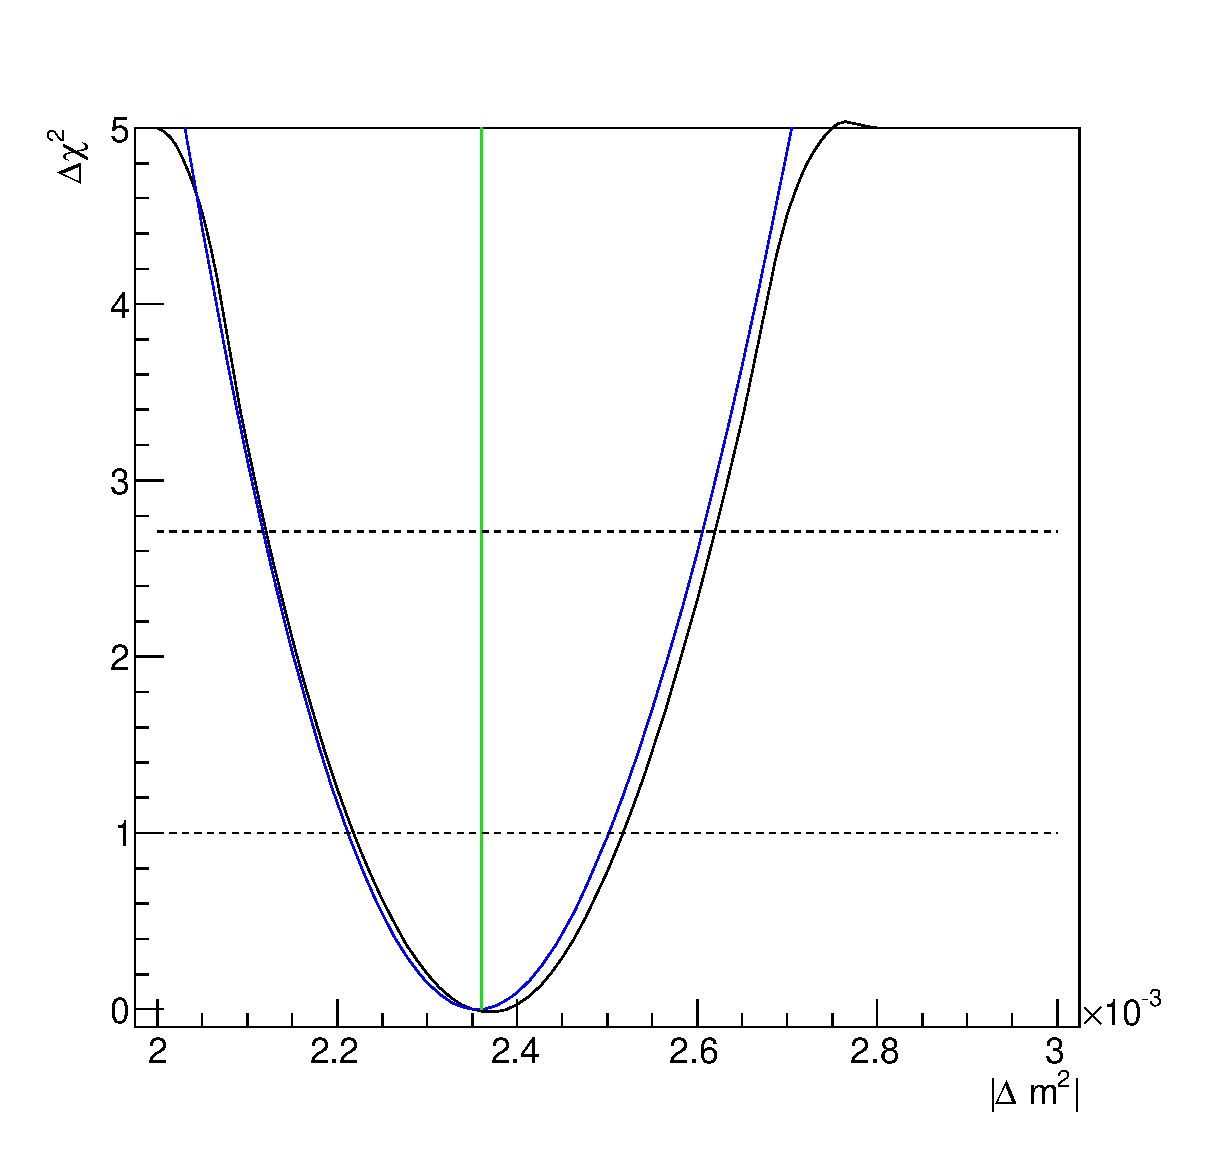
\includegraphics[width=9pc]{./images/appendix/fake_dataset_fits/realistic_fake_dataset0_chisq_dm23sq_global_min.eps}
\caption {
  $\Delta\chi^2$ as function of $|\Delta m^{2}|$ for fake dataset \#6.
  At each point, $\chi^2$ was minimized with respect to 
  $\sin^{2}\theta_{23}$, $\sin^{2}\theta_{13}$, $\delta_{CP}$
  and all relevant nuisance parameters for the joint analysis (black)
  and with respect to $\sin^{2}\theta_{23}$ and all relevant nuisance
  parameters for the disappearance analysis (blue).
}
\label{fig:toymc6_dchisq_Dmsq}
\end{minipage}
\hspace{0.02\linewidth}
\begin{minipage}[t]{0.22\linewidth}
\center
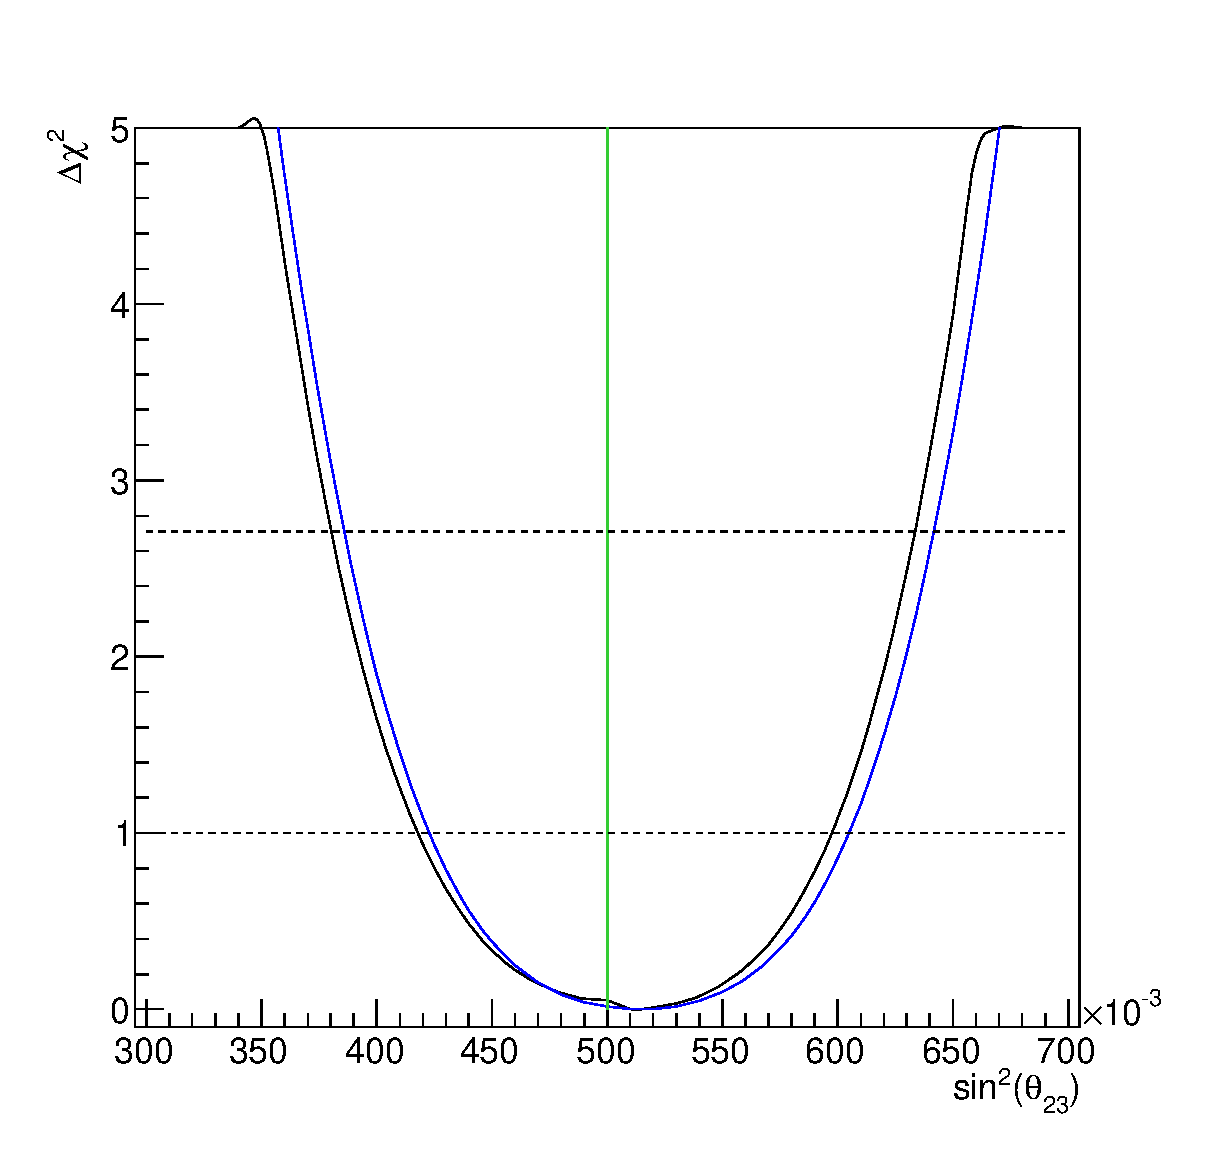
\includegraphics[width=9pc]{./images/appendix/fake_dataset_fits/realistic_fake_dataset0_chisq_theta23_global_min.eps}
\caption {
  $\Delta\chi^2$ as function of $sin^{2}\theta_{23}$ for fake dataset \#6.
  At each point, $\chi^2$ was minimized with respect to 
  $|\Delta m^{2}|$, $\sin^{2}\theta_{13}$, $\delta_{CP}$
  and all relevant nuisance parameters for the joint analysis (black)
  and with respect to $\sin^{2}\theta_{23}$ and all relevant nuisance
  parameters for the disappearance analysis (blue).
}
\label{fig:toymc6_dchisq_sinsqtheta23}
\end{minipage}
\hspace{0.02\linewidth}
\begin{minipage}[t]{0.22\linewidth}
\center
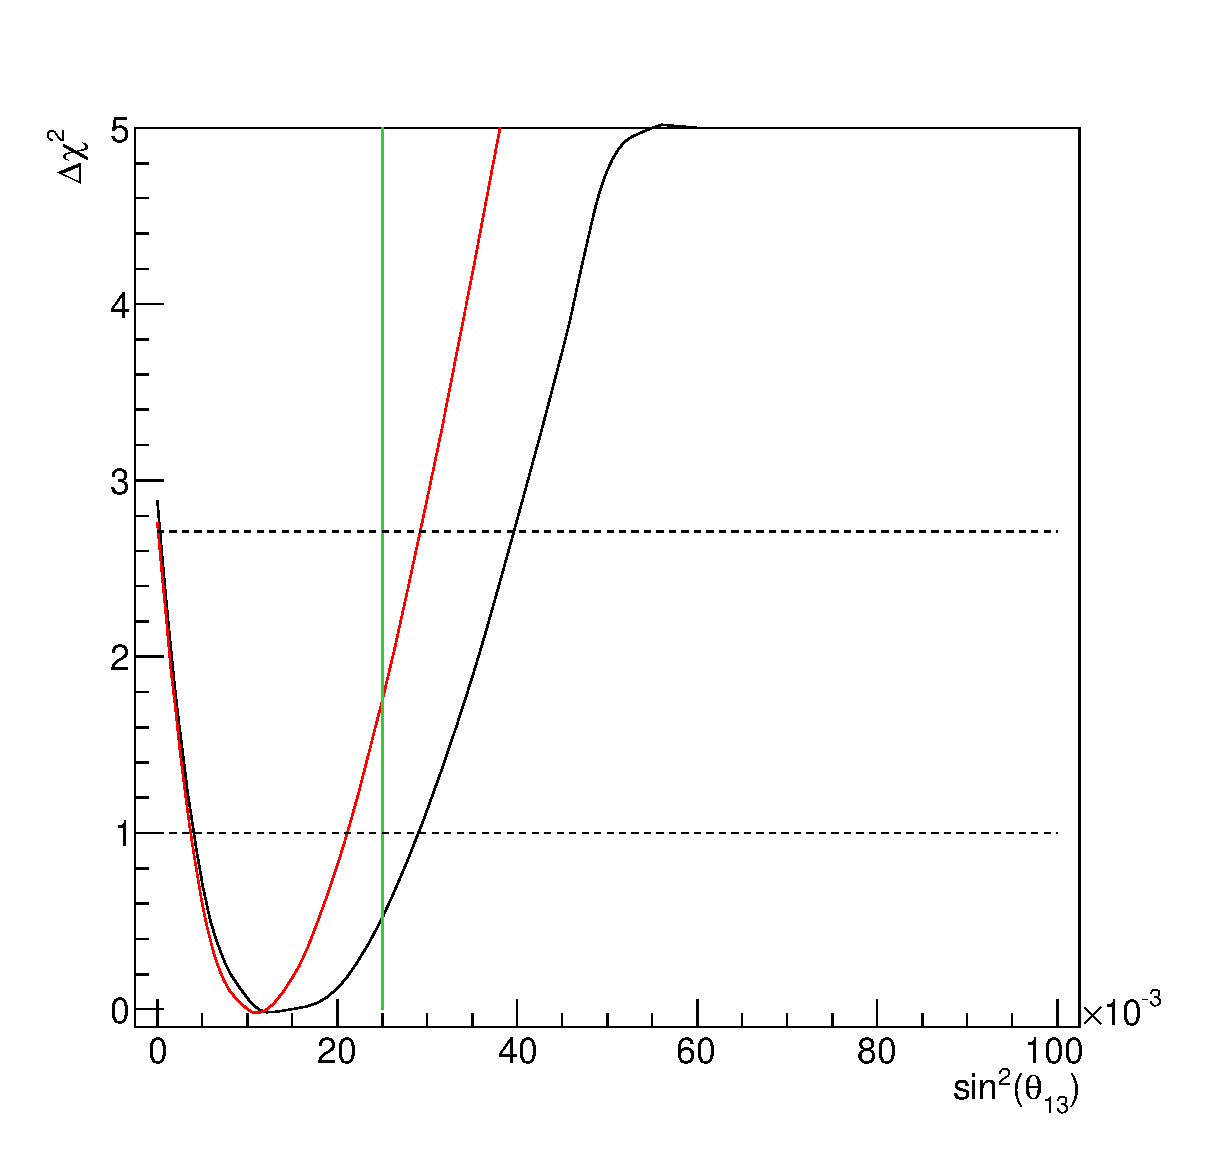
\includegraphics[width=9pc]{./images/appendix/fake_dataset_fits/realistic_fake_dataset0_chisq_theta13_global_min.eps}
\caption {
  $\Delta\chi^2$ as function of $sin^{2}\theta_{13}$ for fake dataset \#6.
  At each point, $\chi^2$ was minimized with respect to 
  $\sin^{2}\theta_{23}$, $\sin^{2}\theta_{13}$, $\delta_{CP}$
  and all relevant nuisance parameters for the joint analysis (black)
  and with respect to all relevant nuisance parameters 
  ($\delta_{CP}$ is fixed to 0) for the appearance analysis (red).
}
\label{fig:toymc6_dchisq_sinsqtheta13}
\end{minipage}
\hspace{0.02\linewidth}
\begin{minipage}[t]{0.22\linewidth}
\center
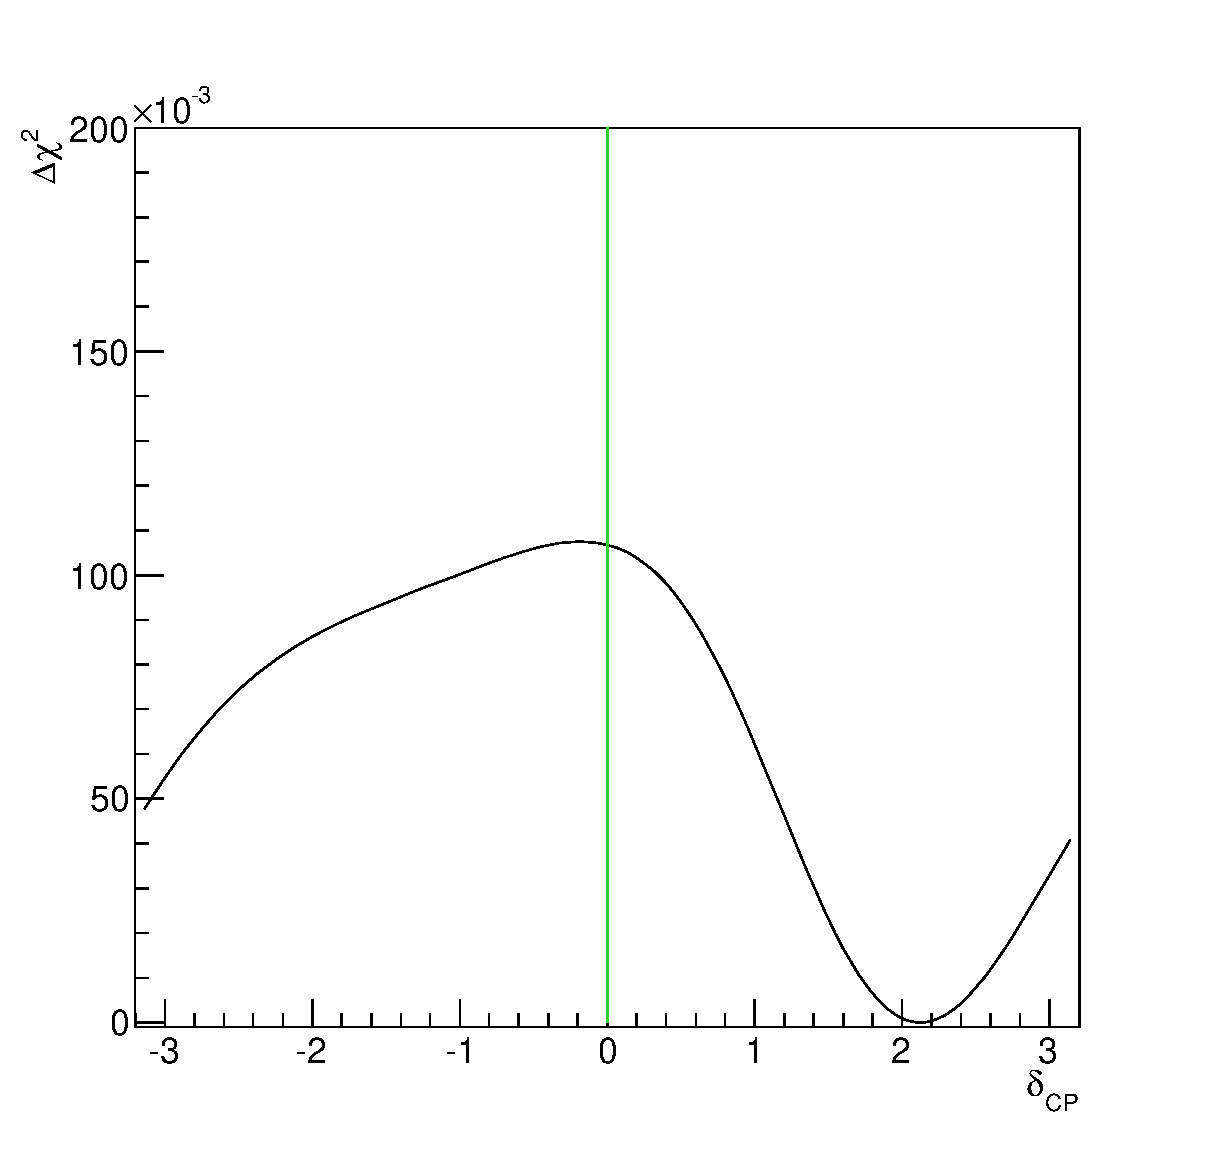
\includegraphics[width=9pc]{.//images/appendix/fake_dataset_fits/realistic_fake_dataset0_chisq_deltacp_global_min.eps}
\caption {
  $\Delta\chi^2$ as function of $\delta_{CP}$ for fake dataset \#6.
  At each point, $\chi^2$ was minimized with respect to 
  all oscillation parameters not shown (and not considered to be fixed)
  and all relevant nuisance parameters.
}
\label{fig:toymc6_dchisq_deltacp}
\end{minipage}
\vfill
\vspace*{0.7cm}
\begin{minipage}[t]{0.48\linewidth}
\center
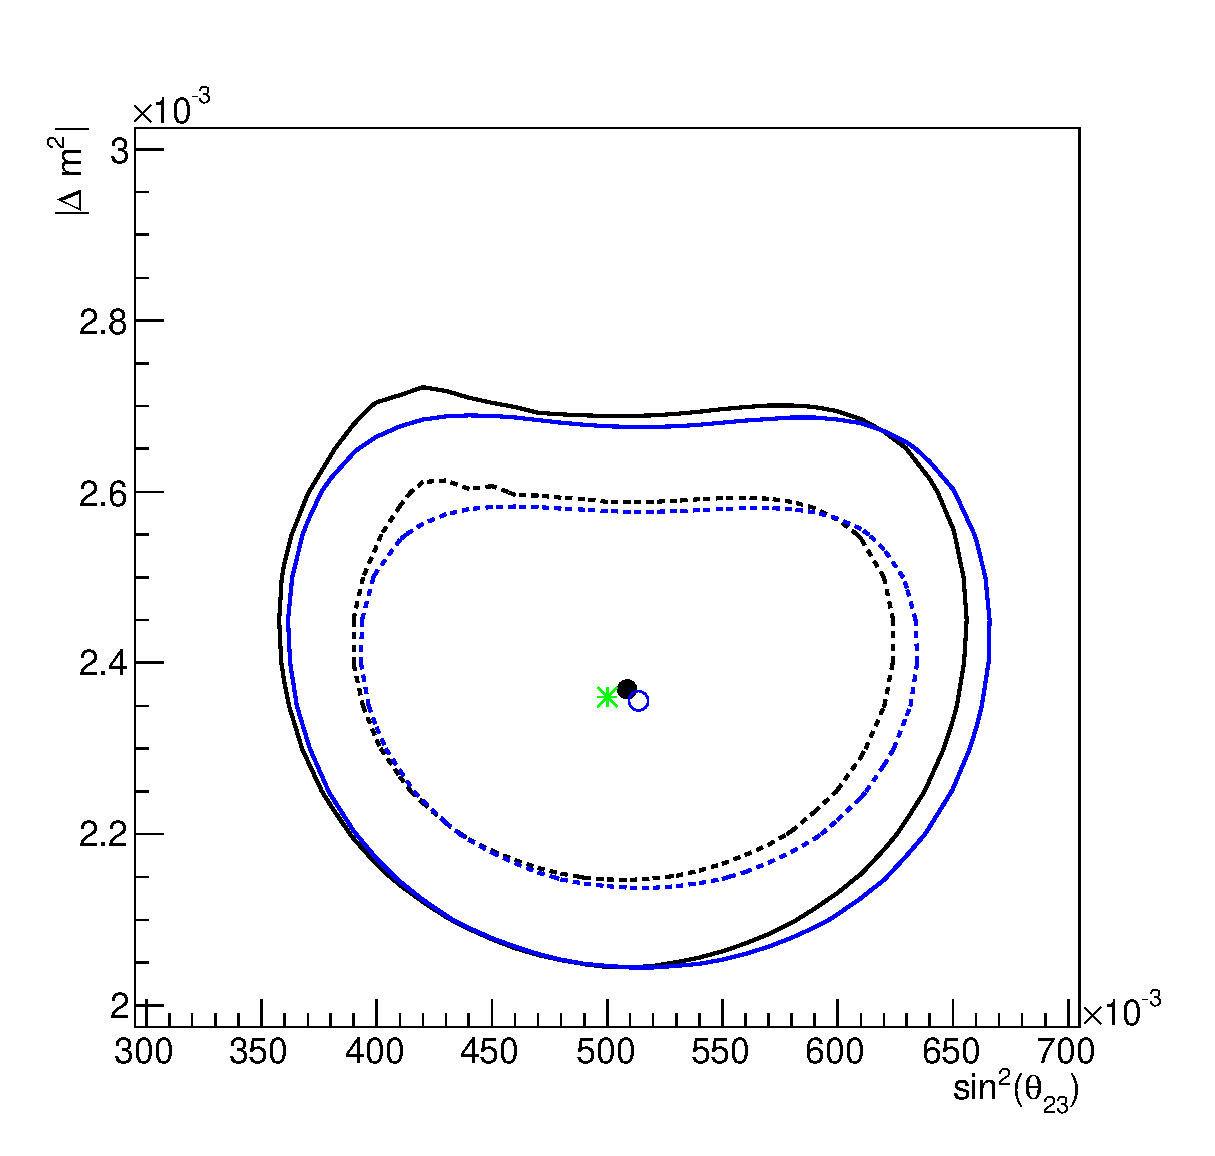
\includegraphics[width=15pc]{./images/appendix/fake_dataset_fits/realistic_fake_dataset0_chisq_theta23_dm23sq_global_min.eps}
\caption {
  68\% and 90\% CL regions in ($sin^{2}\theta_{23}$, $|\Delta m^{2}|$) space for fake dataset \#6.
  At each point, $\chi^2$ was minimized with respect to 
  $\sin^{2}\theta_{13}$, $\delta_{CP}$
  and all relevant nuisance parameters for the joint analysis (black)
  and with respect to all relevant nuisance parameters for the disappearance analysis (blue).
}
\label{fig:toymc6_confreg_sinsqtheta23_Dmsq}
\end{minipage}
\hspace{0.03\linewidth}
\begin{minipage}[t]{0.48\linewidth}
\center
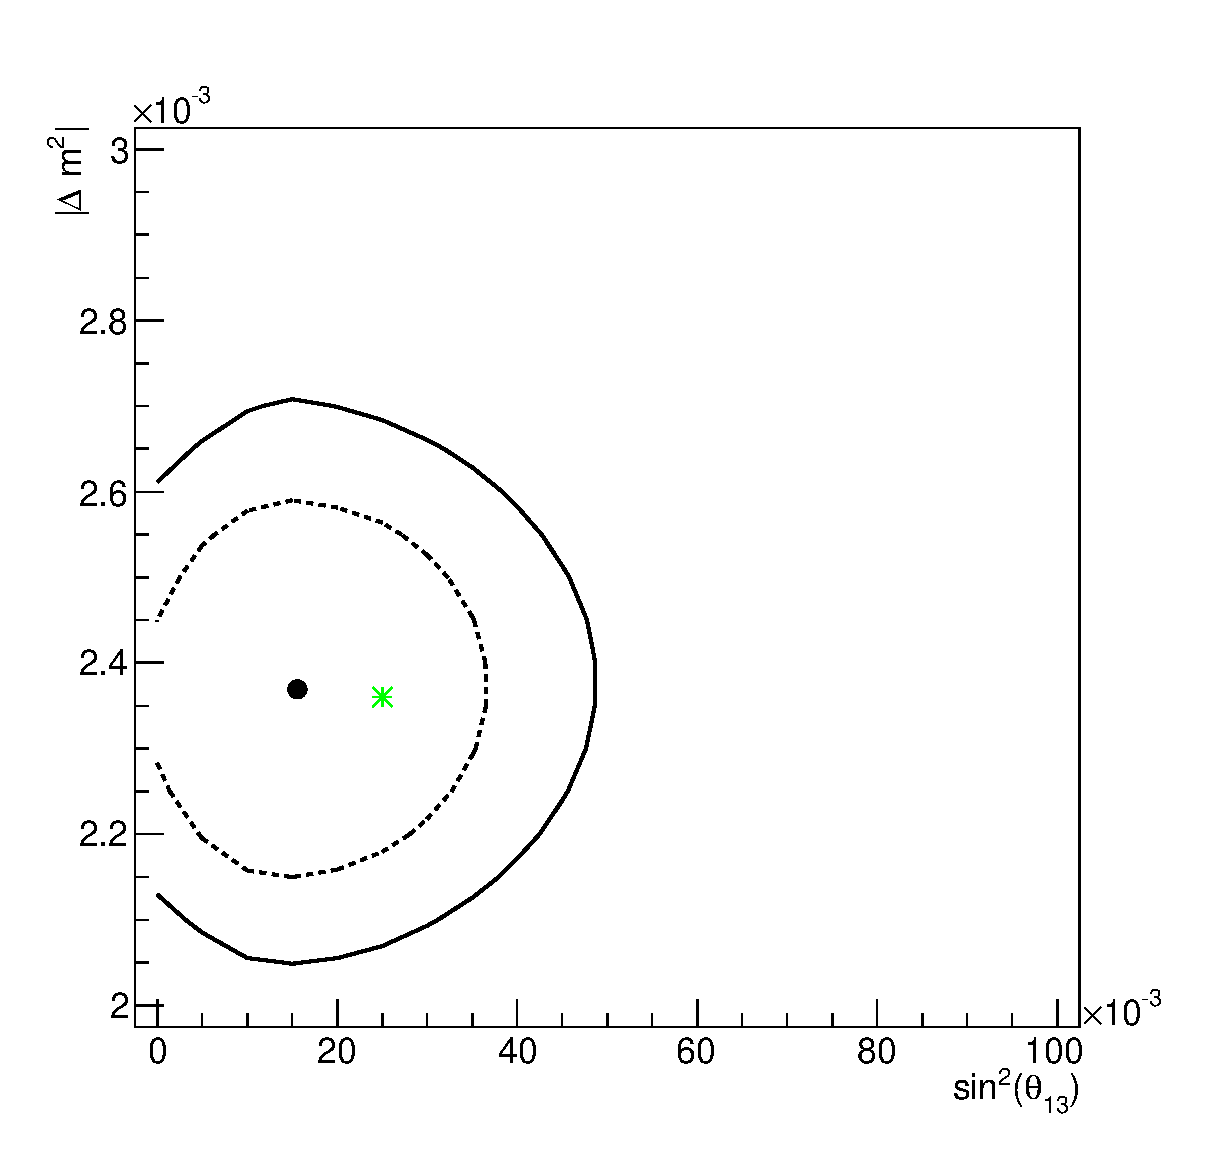
\includegraphics[width=15pc]{./images/appendix/fake_dataset_fits/realistic_fake_dataset0_chisq_theta13_dm23sq_global_min.eps}
\caption {
  68\% and 90\% CL regions in ($sin^{2}\theta_{13}$, $|\Delta m^{2}|$) space for fake dataset \#6.
  At each point, $\chi^2$ was minimized with respect to 
  all oscillation parameters not shown (and not considered to be fixed)
  and all relevant nuisance parameters.
}
\label{fig:toymc6_confreg_sinsqtheta13_Dmsq}
\end{minipage}

\vfill
\vspace*{0.7cm}

\begin{minipage}[t]{0.48\linewidth}
\center
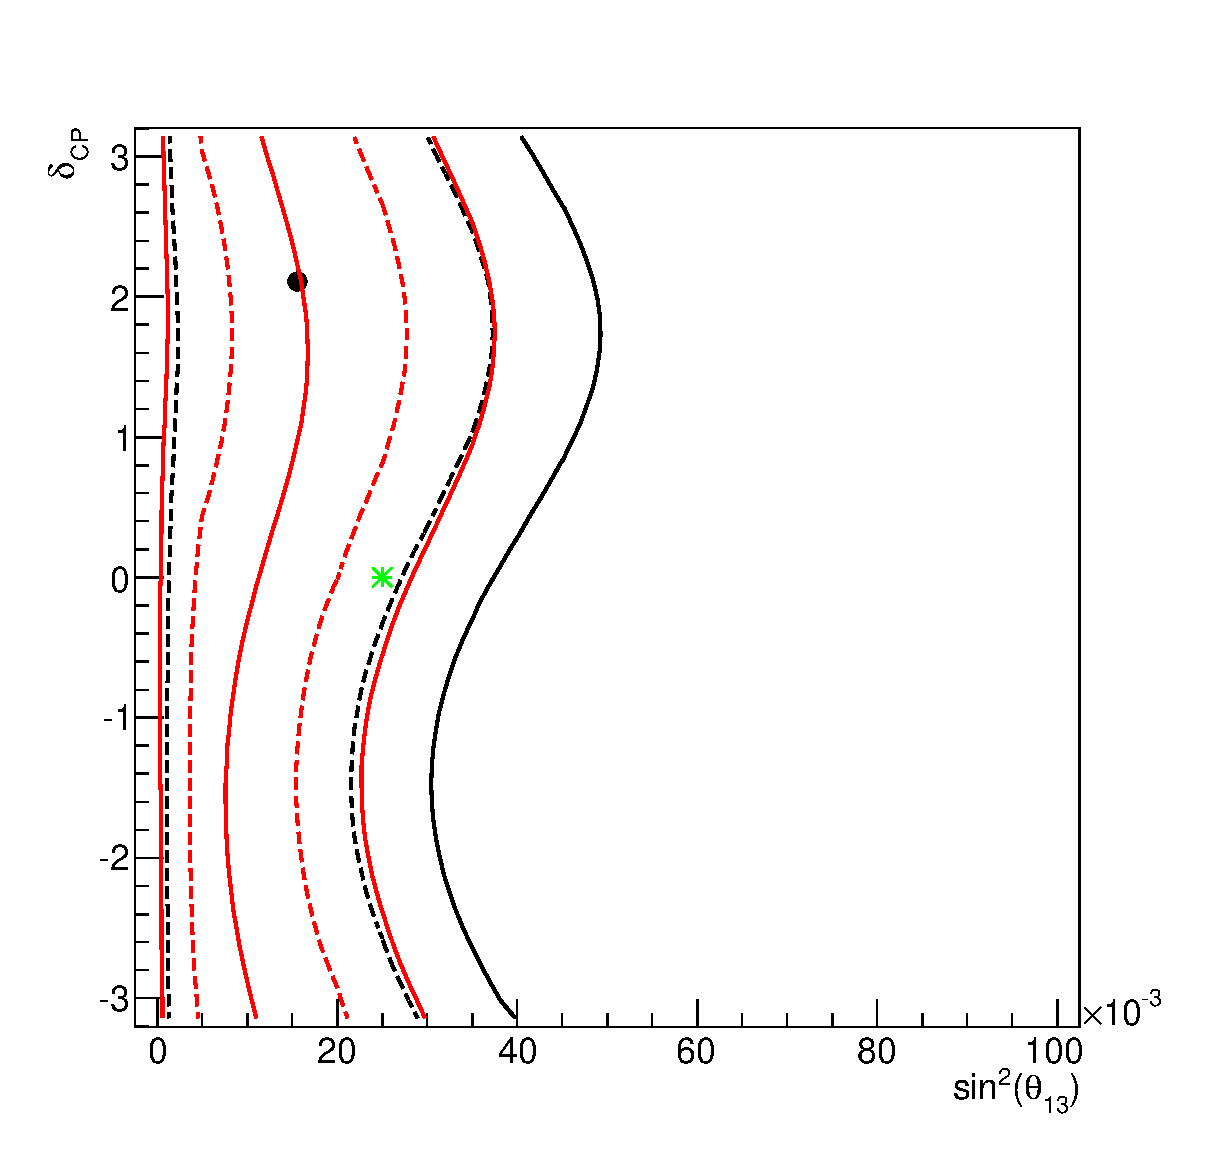
\includegraphics[width=15pc]{./images/appendix/fake_dataset_fits/realistic_fake_dataset0_chisq_theta13_deltacp_global_min.eps}
\caption {
  68\% and 90\% CL regions in ($sin^{2}\theta_{13}$, $\delta_{CP}$) space for fake dataset \#6.
  At each point, $\chi^2$ was minimized with respect to 
  $|\Delta m^{2}|$, $\sin^{2}\theta_{23}$
  and all relevant nuisance parameters for the joint analysis (black)
  and with respect to all relevant nuisance parameters for the appearance analysis (red).
  Notice that different methods are used to
  construct confidence regions for the joint analysis (global minimum) and for the 
  stand-alone appearance analysis (raster scan).
}
\label{fig:toymc6_confreg_sinsqtheta13_deltacp}
\end{minipage}
\hspace{0.03\linewidth}
\begin{minipage}[t]{0.48\linewidth}
\center
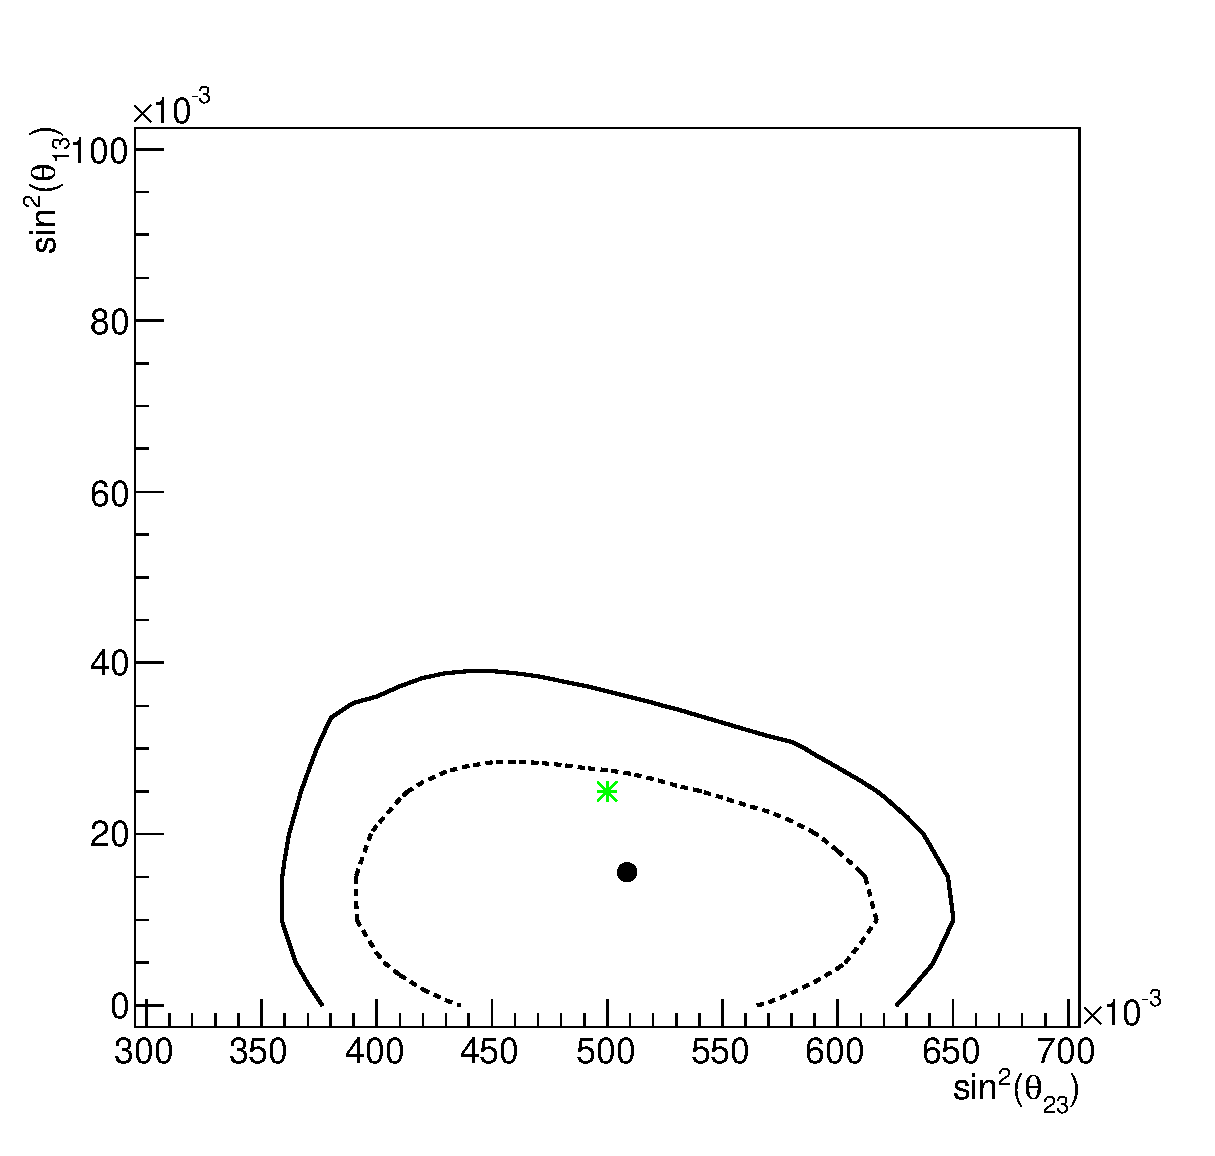
\includegraphics[width=15pc]{./images/appendix/fake_dataset_fits/realistic_fake_dataset0_chisq_theta13_theta23_global_min.eps}
\caption {
  68\% and 90\% CL regions in ($sin^{2}\theta_{23}$, $sin^{2}\theta_{13}$) space for fake dataset \#6.
  At each point, $\chi^2$ was minimized with respect to 
  all oscillation parameters not shown (and not considered to be fixed)
  and all relevant nuisance parameters.
}
\label{fig:toymc6_confreg_sinsqtheta23_sinsqtheta13}
\end{minipage}

\end{figure*}




% 
% 
% ..............................................
% Fake dataset #7
% 
%
\clearpage

\begin{figure*}[htb]

\begin{minipage}[t]{0.46\linewidth}
\center
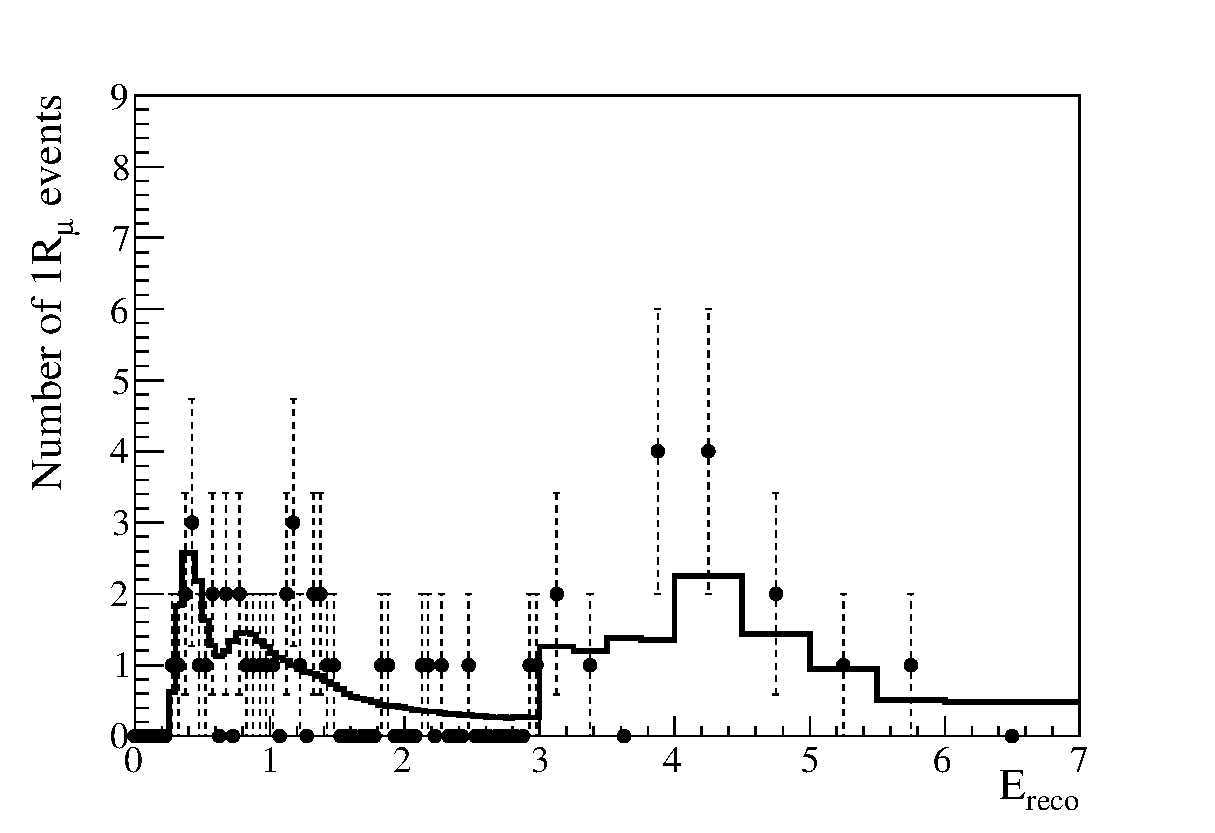
\includegraphics[width=15pc]{./images/appendix/fake_dataset_fits/realistic_fake_dataset1_nh_1st_1Rmu.eps}
\caption {
  Single $\mu$-like ring event best-fit reconstructed energy spectrum
  to fake dataset \#7.
}
\label{fig:toymc7_1Rmu_bestfit_spectrum}
\end{minipage}
\hspace{0.03\linewidth}
\begin{minipage}[t]{0.46\linewidth}
\center
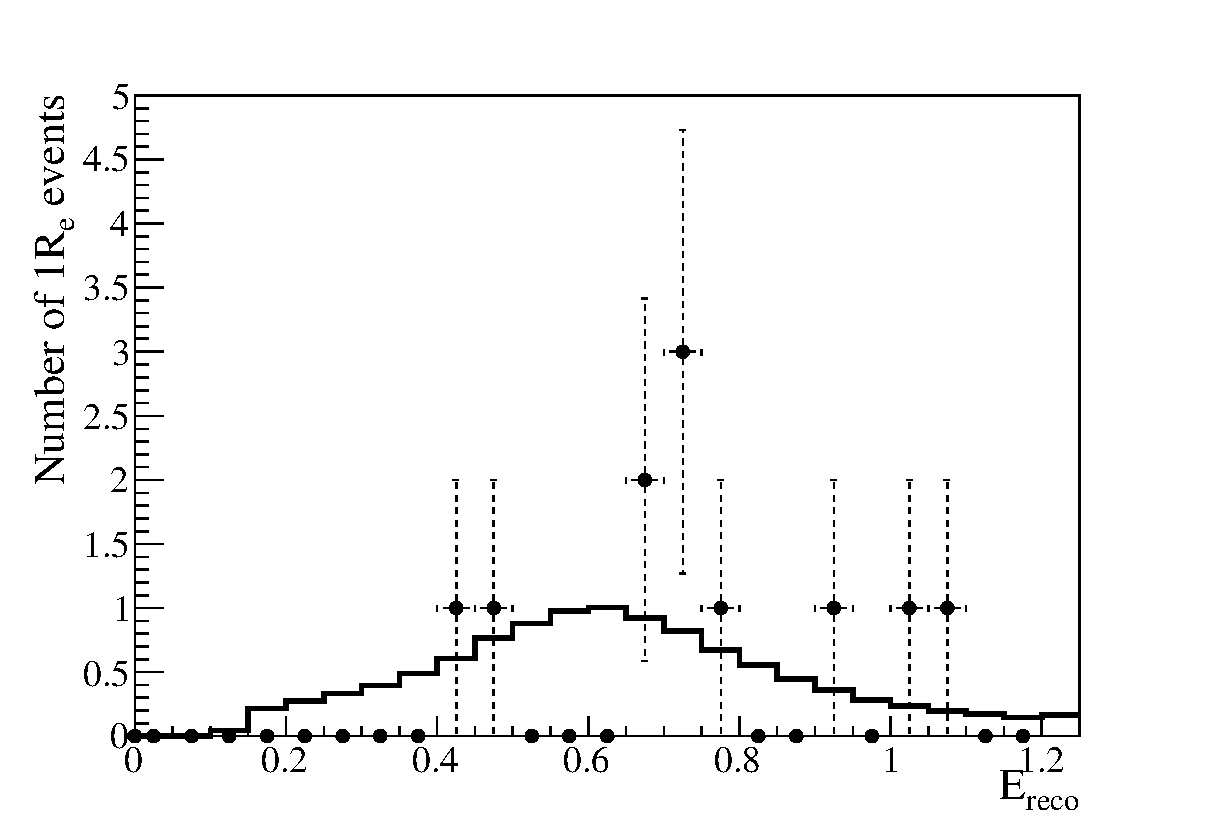
\includegraphics[width=15pc]{./images/appendix/fake_dataset_fits/realistic_fake_dataset1_nh_1st_1Re.eps}
\caption {
  Single e-like ring event best-fit reconstructed energy spectrum
  to fake dataset \#7.
}
\label{fig:toymc7_1Re_bestfit_spectrum}
\end{minipage}

\vfill
\vspace*{0.7cm}

\begin{minipage}[t]{0.90\linewidth}
\center
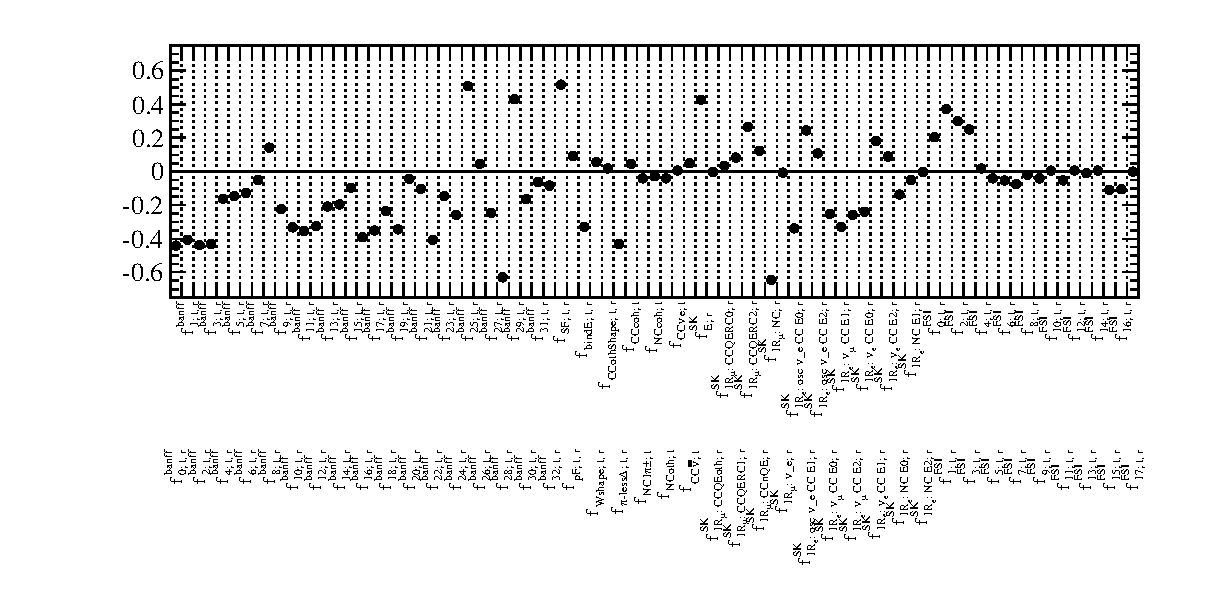
\includegraphics[width=30pc,angle=270]{./images/appendix/fake_dataset_fits/pulls_realistic_fake_dataset1_nh_1st.eps}
\caption {
  Systematic parameter pulls for the oscillation fit to fake dataset \#7.
}
\label{fig:toymc7_pulls}
\end{minipage}

\end{figure*}



%...........................................................
%
% chisq distributions used for calculating the fit p-values
%

\begin{figure*}[htb]

\begin{minipage}[t]{0.90\linewidth}
\center
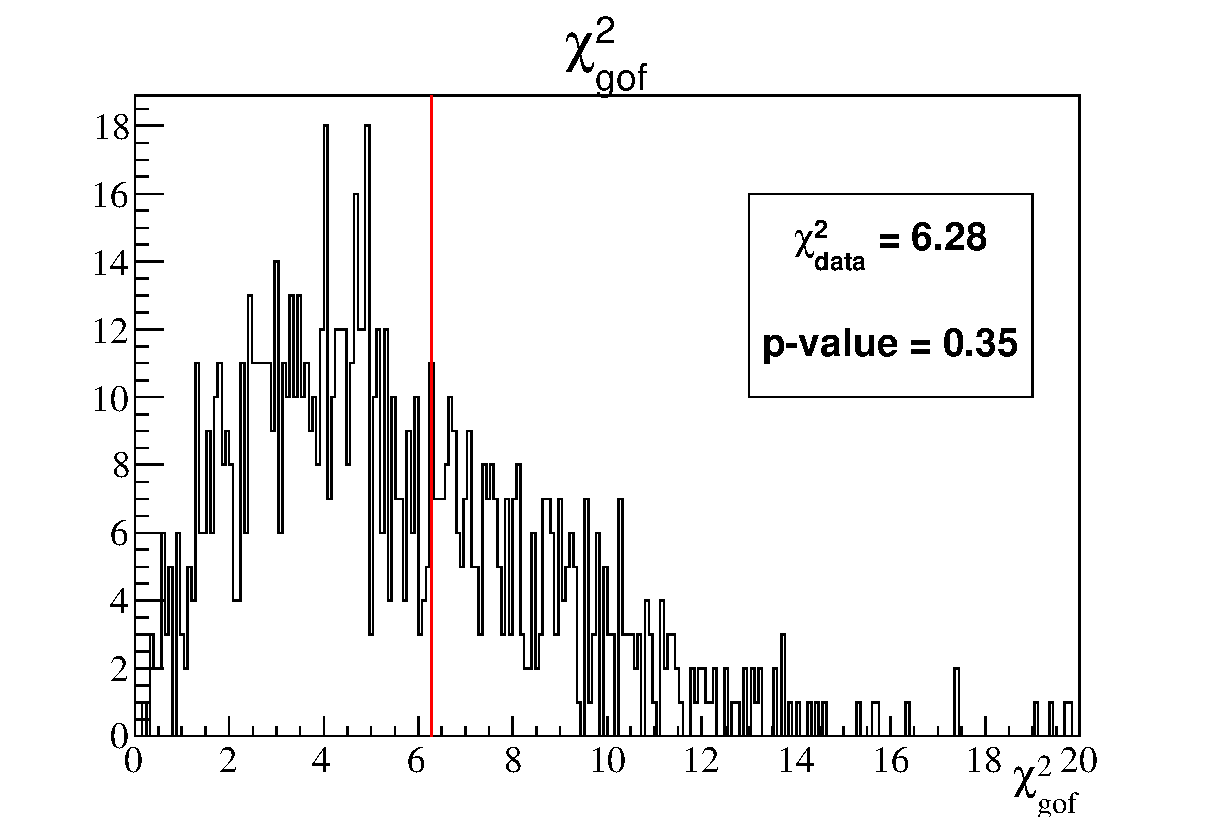
\includegraphics[width=30pc]{./images/appendix/fake_dataset_fits/realistic_fake_dataset1_nh_1st_gof_new.eps}
\caption {
  Distribution of $\chi^2_{gof}$, the goodness-of-fit (gof) $\chi^2$, 
  from 1k toy MC experiments generated at dataset \#7 joint 3-flavour analysis best-fit oscillation point.
  The $\chi^2_{gof}$ value for the dataset \#7 ($\chi^2_{data}$) is highlighted.
  All $\chi^2_{gof}$ values were computed 
  using the 5 (single $\mu$-like ring) + 3 (single e-like ring) 
  reconstructed energy binning scheme described in Sec.\ \ref{sec:goodness_of_fit}.
}
\label{fig:toymc7_gofchisq}
\end{minipage}

\vfill
\vspace*{0.7cm}

\begin{minipage}[t]{0.46\linewidth}
\center
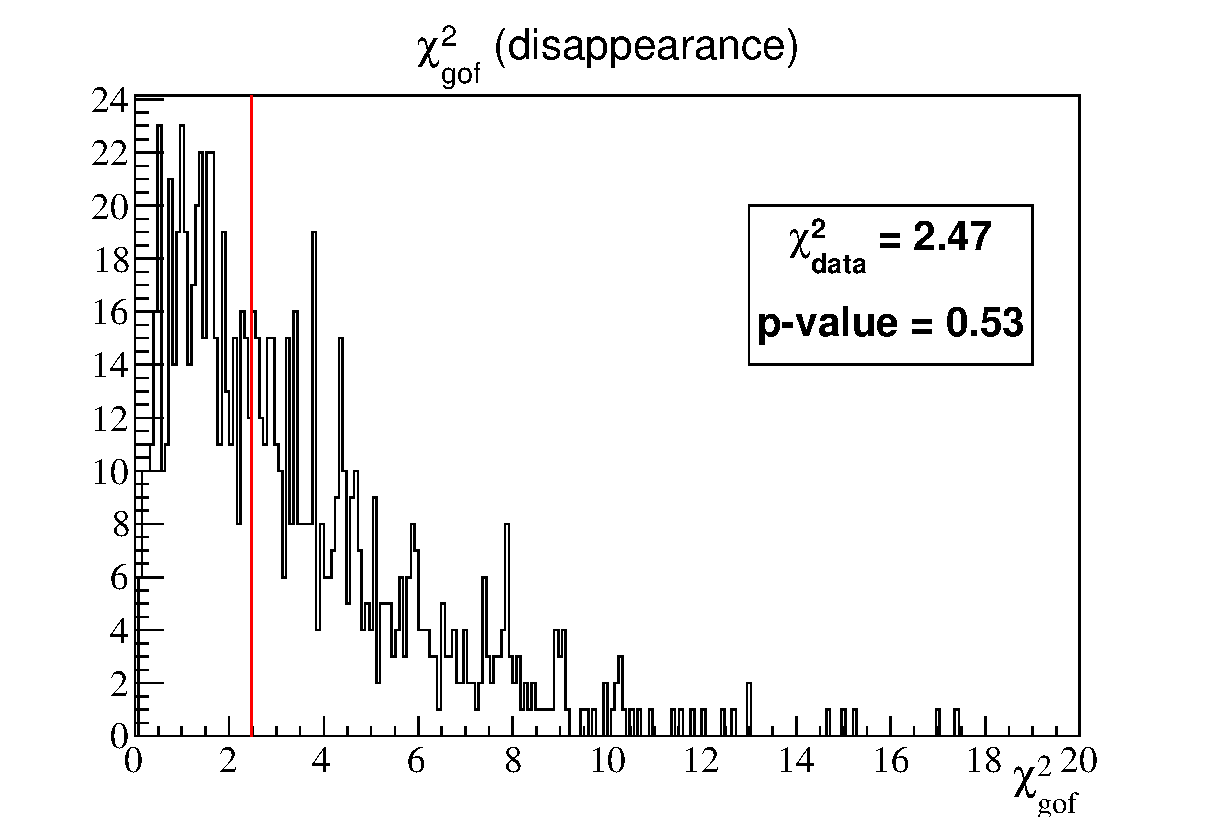
\includegraphics[width=18pc]{./images/appendix/fake_dataset_fits/realistic_fake_dataset1_nh_1st_gof_disap_new.eps}
\caption {
  Distribution of $\chi^2_{gof}$
  from 1k toy MC experiments generated at the dataset \#7 stand-alone 3-flavour $\nu_{\mu}$ disappearance analysis best-fit oscillation point.
  The $\chi^2_{gof}$ value for the dataset \#7 ($\chi^2_{data}$) is highlighted.
  All $\chi^2_{gof}$ values were computed 
  using the 5 (single $\mu$-like ring) 
  reconstructed energy binning scheme described in Sec.\ \ref{sec:goodness_of_fit}.
}
\label{fig:toymc7_gofchisq_disapp}
\end{minipage}
\hspace{0.03\linewidth}
\begin{minipage}[t]{0.46\linewidth}
\center
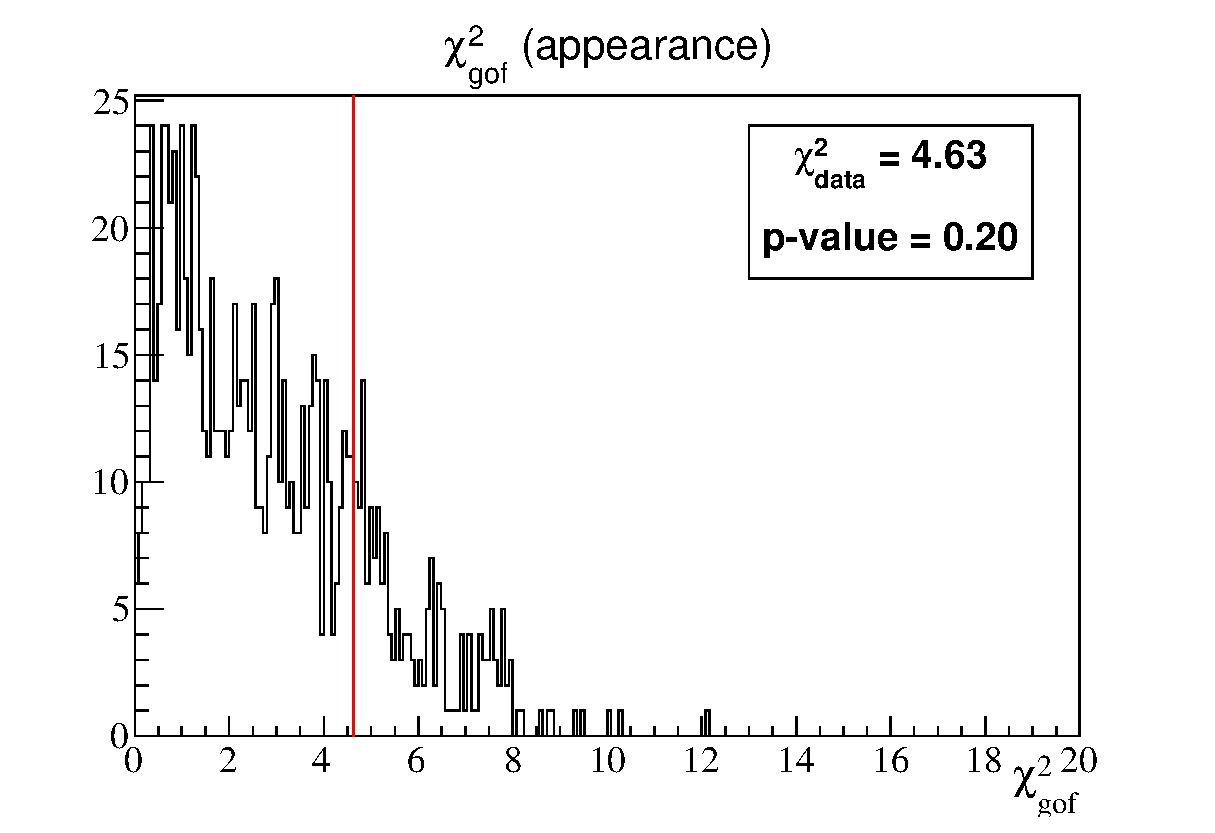
\includegraphics[width=18pc]{./images/appendix/fake_dataset_fits/realistic_fake_dataset1_nh_1st_gof_app_new.eps}
\caption {
  Distribution of $\chi^2_{gof}$
  from 1k toy MC experiments generated at the dataset \#7 stand-alone 3-flavour $\nu_{e}$ appearance analysis best-fit oscillation point.
  The $\chi^2_{gof}$ value for the dataset \#7 ($\chi^2_{data}$) is highlighted.
  All $\chi^2_{gof}$ values were computed 
  using the 3 (single e-like ring) 
  reconstructed energy binning scheme  as described in Sec.\ \ref{sec:goodness_of_fit}.
}
\label{fig:toymc7_gofchisq_app}
\end{minipage}

\end{figure*}



%
% delta\chisq and contours
%

\begin{figure*}[htb]

\begin{minipage}[t]{0.22\linewidth}
\center
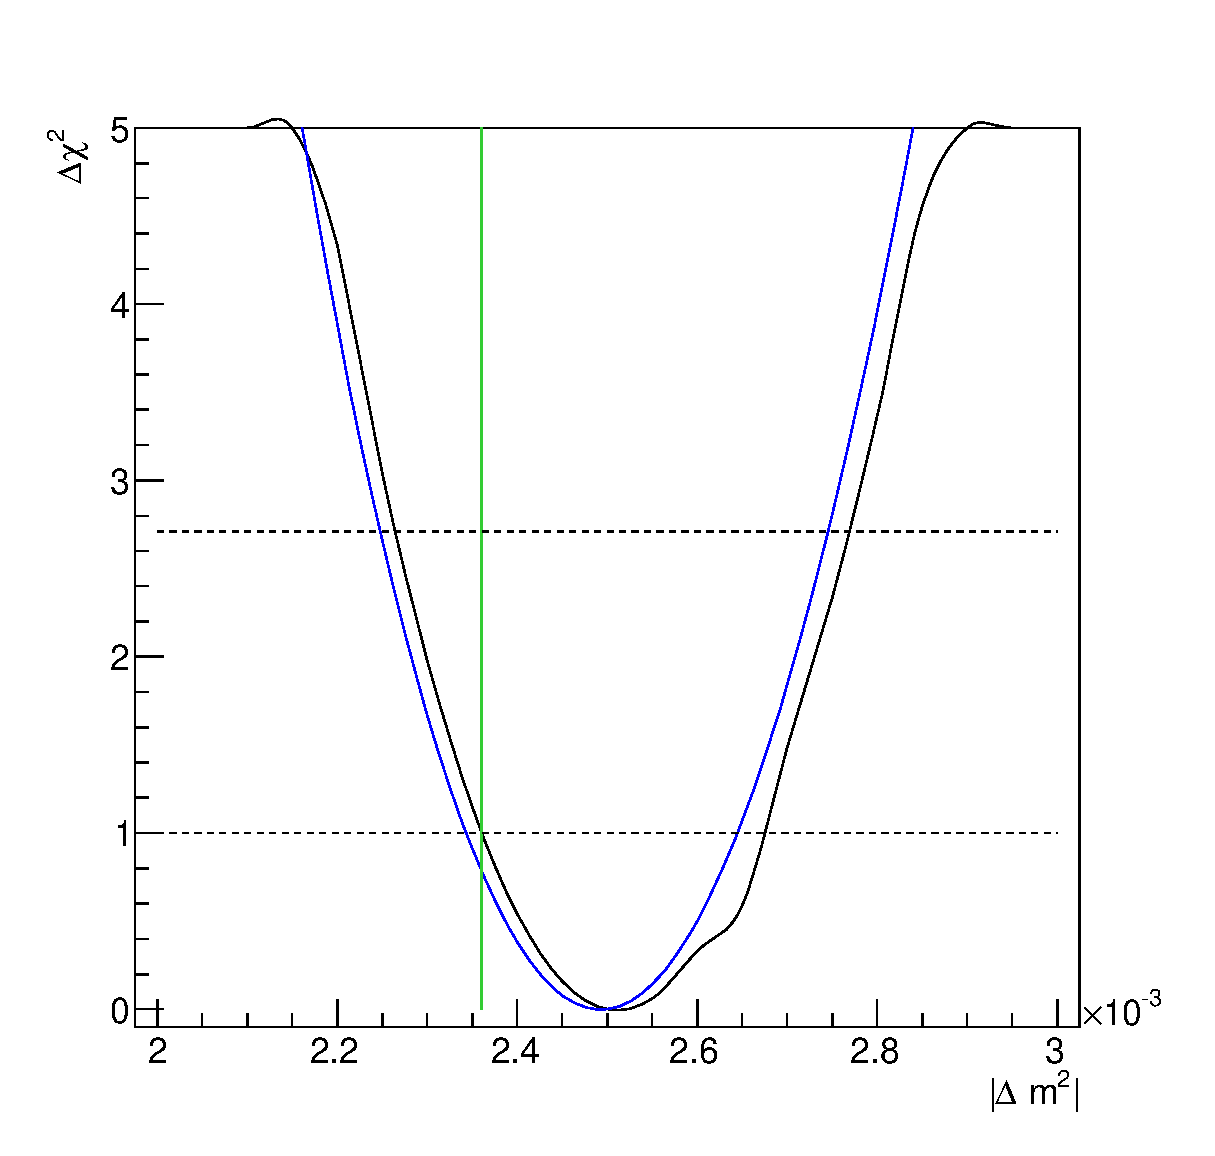
\includegraphics[width=9pc]{./images/appendix/fake_dataset_fits/realistic_fake_dataset1_chisq_dm23sq_global_min.eps}
\caption {
  $\Delta\chi^2$ as function of $|\Delta m^{2}|$ for fake dataset \#7.
  At each point, $\chi^2$ was minimized with respect to 
  $\sin^{2}\theta_{23}$, $\sin^{2}\theta_{13}$, $\delta_{CP}$
  and all relevant nuisance parameters for the joint analysis (black)
  and with respect to $\sin^{2}\theta_{23}$ and all relevant nuisance
  parameters for the disappearance analysis (blue).
}
\label{fig:toymc7_dchisq_Dmsq}
\end{minipage}
\hspace{0.02\linewidth}
\begin{minipage}[t]{0.22\linewidth}
\center
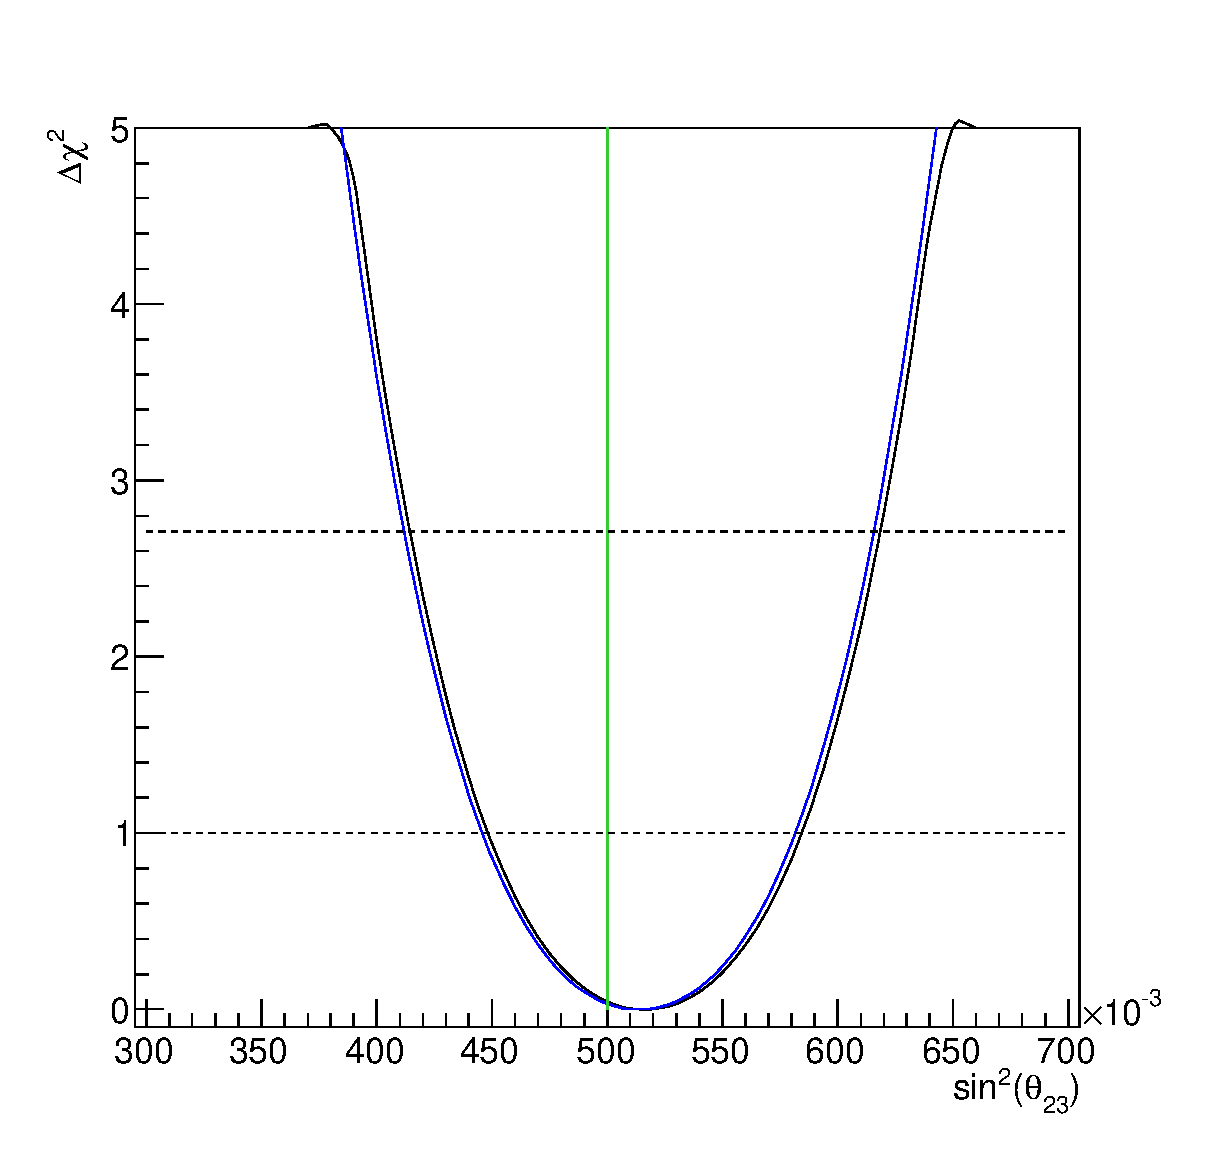
\includegraphics[width=9pc]{./images/appendix/fake_dataset_fits/realistic_fake_dataset1_chisq_theta23_global_min.eps}
\caption {
  $\Delta\chi^2$ as function of $sin^{2}\theta_{23}$ for fake dataset \#7.
  At each point, $\chi^2$ was minimized with respect to 
  $|\Delta m^{2}|$, $\sin^{2}\theta_{13}$, $\delta_{CP}$
  and all relevant nuisance parameters for the joint analysis (black)
  and with respect to $\sin^{2}\theta_{23}$ and all relevant nuisance
  parameters for the disappearance analysis (blue).
}
\label{fig:toymc7_dchisq_sinsqtheta23}
\end{minipage}
\hspace{0.02\linewidth}
\begin{minipage}[t]{0.22\linewidth}
\center
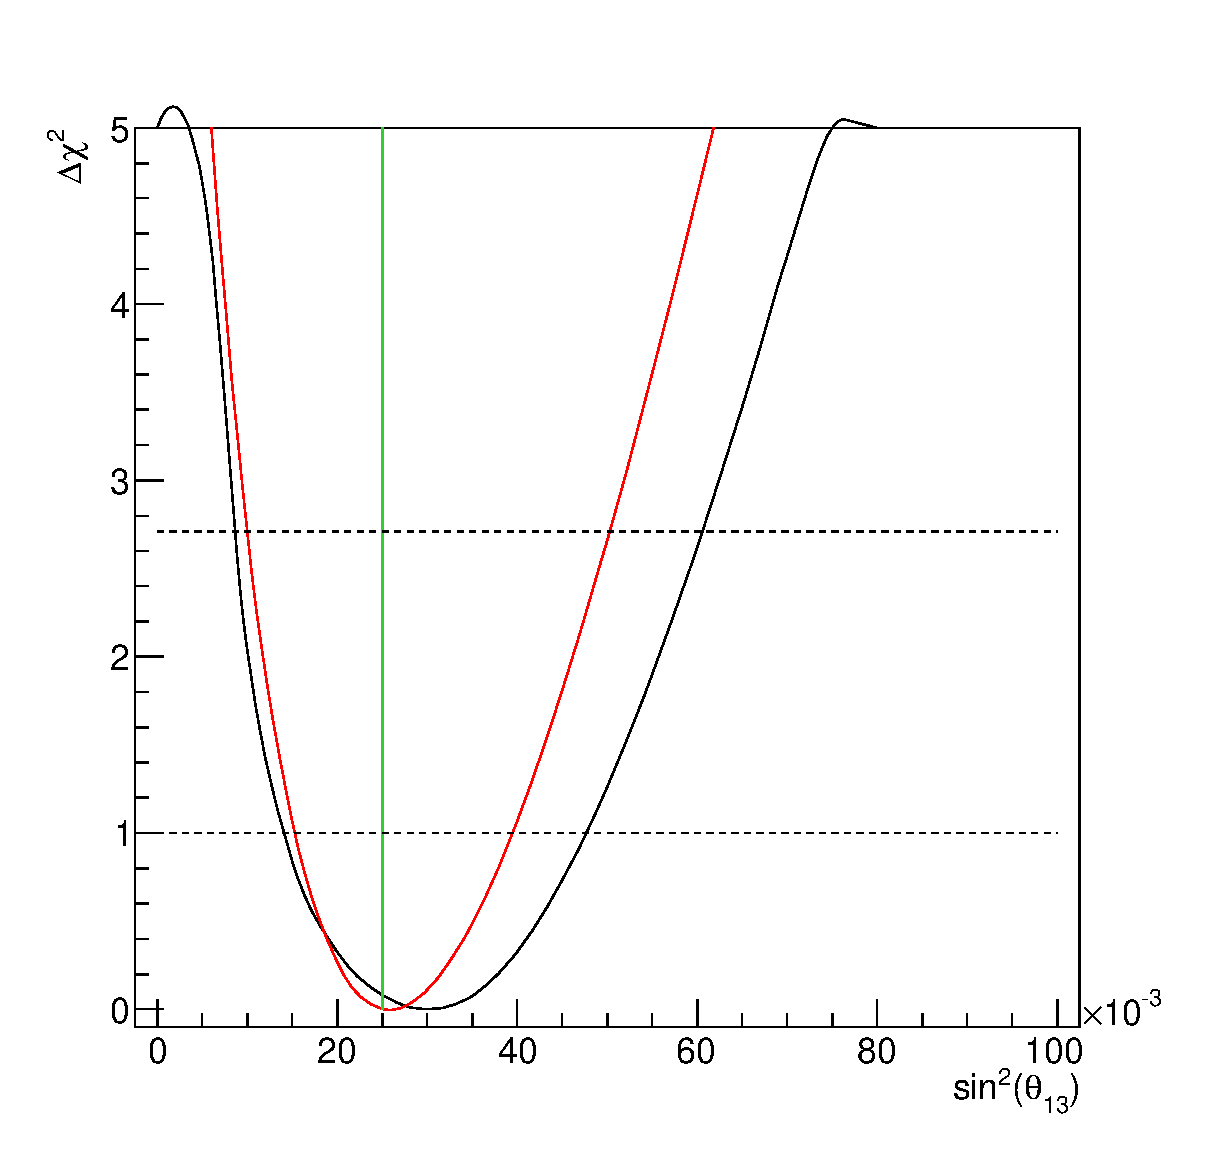
\includegraphics[width=9pc]{./images/appendix/fake_dataset_fits/realistic_fake_dataset1_chisq_theta13_global_min.eps}
\caption {
  $\Delta\chi^2$ as function of $sin^{2}\theta_{13}$ for fake dataset \#7.
  At each point, $\chi^2$ was minimized with respect to 
  $\sin^{2}\theta_{23}$, $\sin^{2}\theta_{13}$, $\delta_{CP}$
  and all relevant nuisance parameters for the joint analysis (black)
  and with respect to all relevant nuisance parameters 
  ($\delta_{CP}$ is fixed to 0) for the appearance analysis (red).
}
\label{fig:toymc7_dchisq_sinsqtheta13}
\end{minipage}
\hspace{0.02\linewidth}
\begin{minipage}[t]{0.22\linewidth}
\center
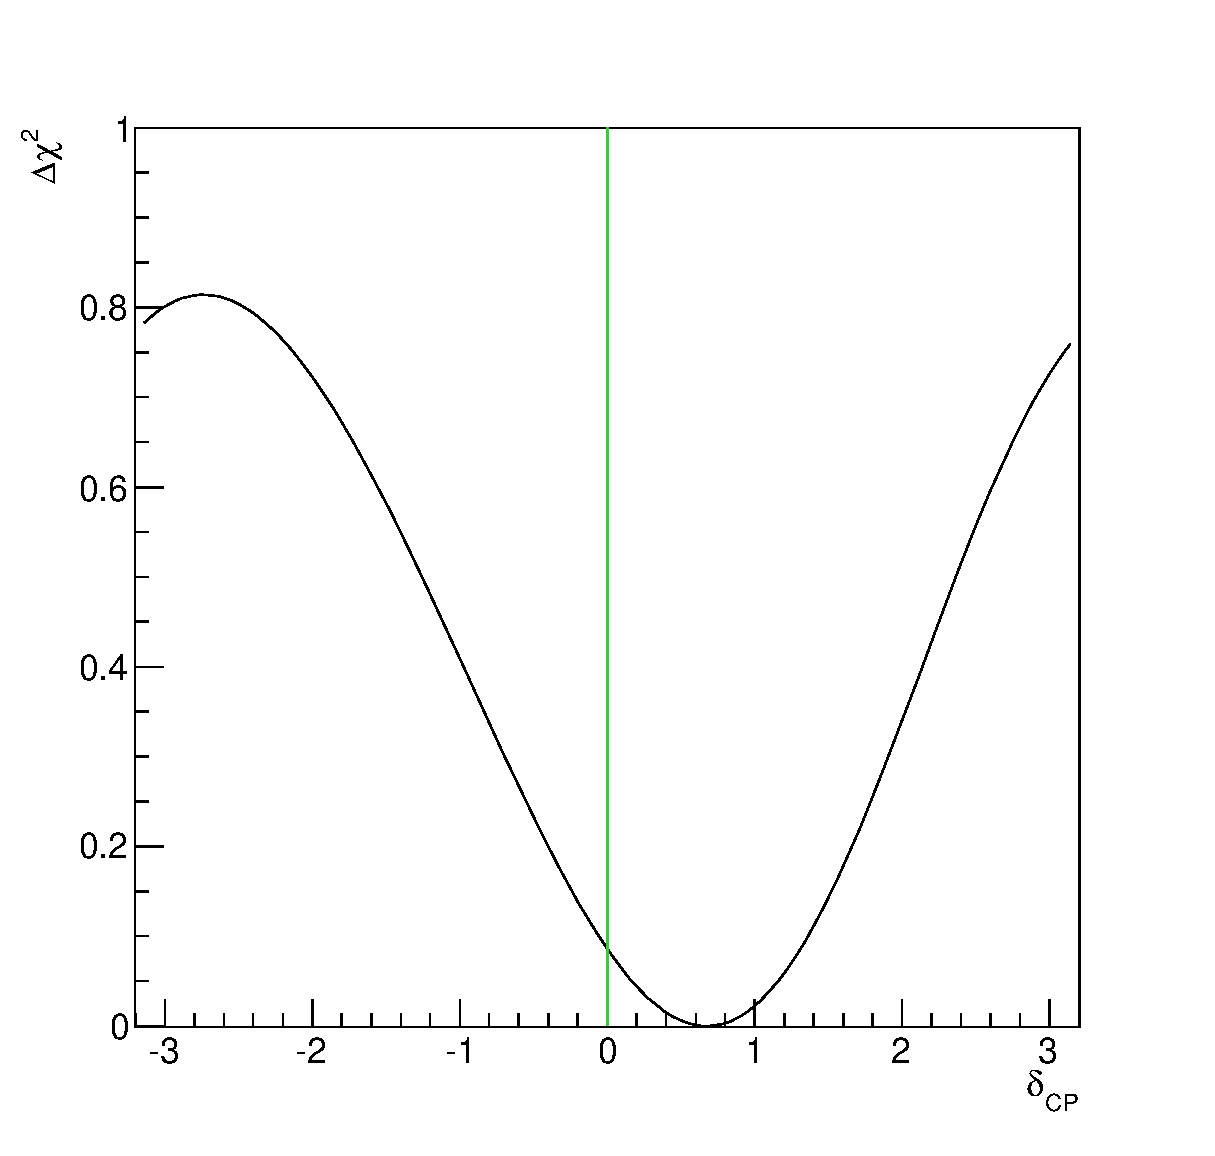
\includegraphics[width=9pc]{.//images/appendix/fake_dataset_fits/realistic_fake_dataset1_chisq_deltacp_global_min.eps}
\caption {
  $\Delta\chi^2$ as function of $\delta_{CP}$ for fake dataset \#7.
  At each point, $\chi^2$ was minimized with respect to 
  all oscillation parameters not shown (and not considered to be fixed)
  and all relevant nuisance parameters.
}
\label{fig:toymc7_dchisq_deltacp}
\end{minipage}
\vfill
\vspace*{0.7cm}
\begin{minipage}[t]{0.48\linewidth}
\center
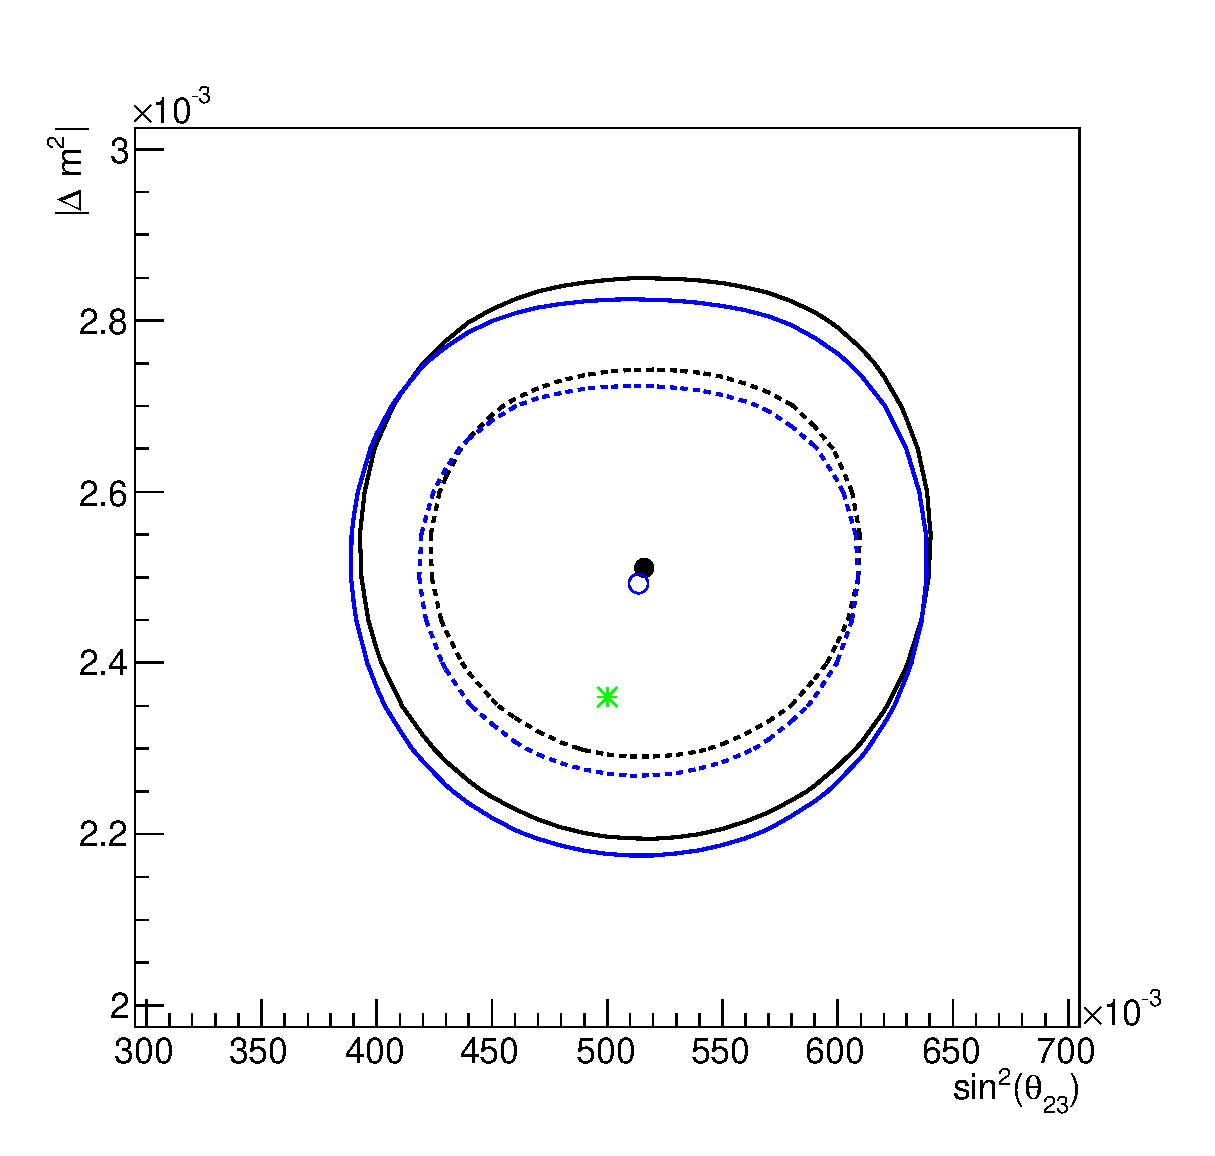
\includegraphics[width=15pc]{./images/appendix/fake_dataset_fits/realistic_fake_dataset1_chisq_theta23_dm23sq_global_min.eps}
\caption {
  68\% and 90\% CL regions in ($sin^{2}\theta_{23}$, $|\Delta m^{2}|$) space for fake dataset \#7.
  At each point, $\chi^2$ was minimized with respect to 
  $\sin^{2}\theta_{13}$, $\delta_{CP}$
  and all relevant nuisance parameters for the joint analysis (black)
  and with respect to all relevant nuisance parameters for the disappearance analysis (blue).
}
\label{fig:toymc7_confreg_sinsqtheta23_Dmsq}
\end{minipage}
\hspace{0.03\linewidth}
\begin{minipage}[t]{0.48\linewidth}
\center
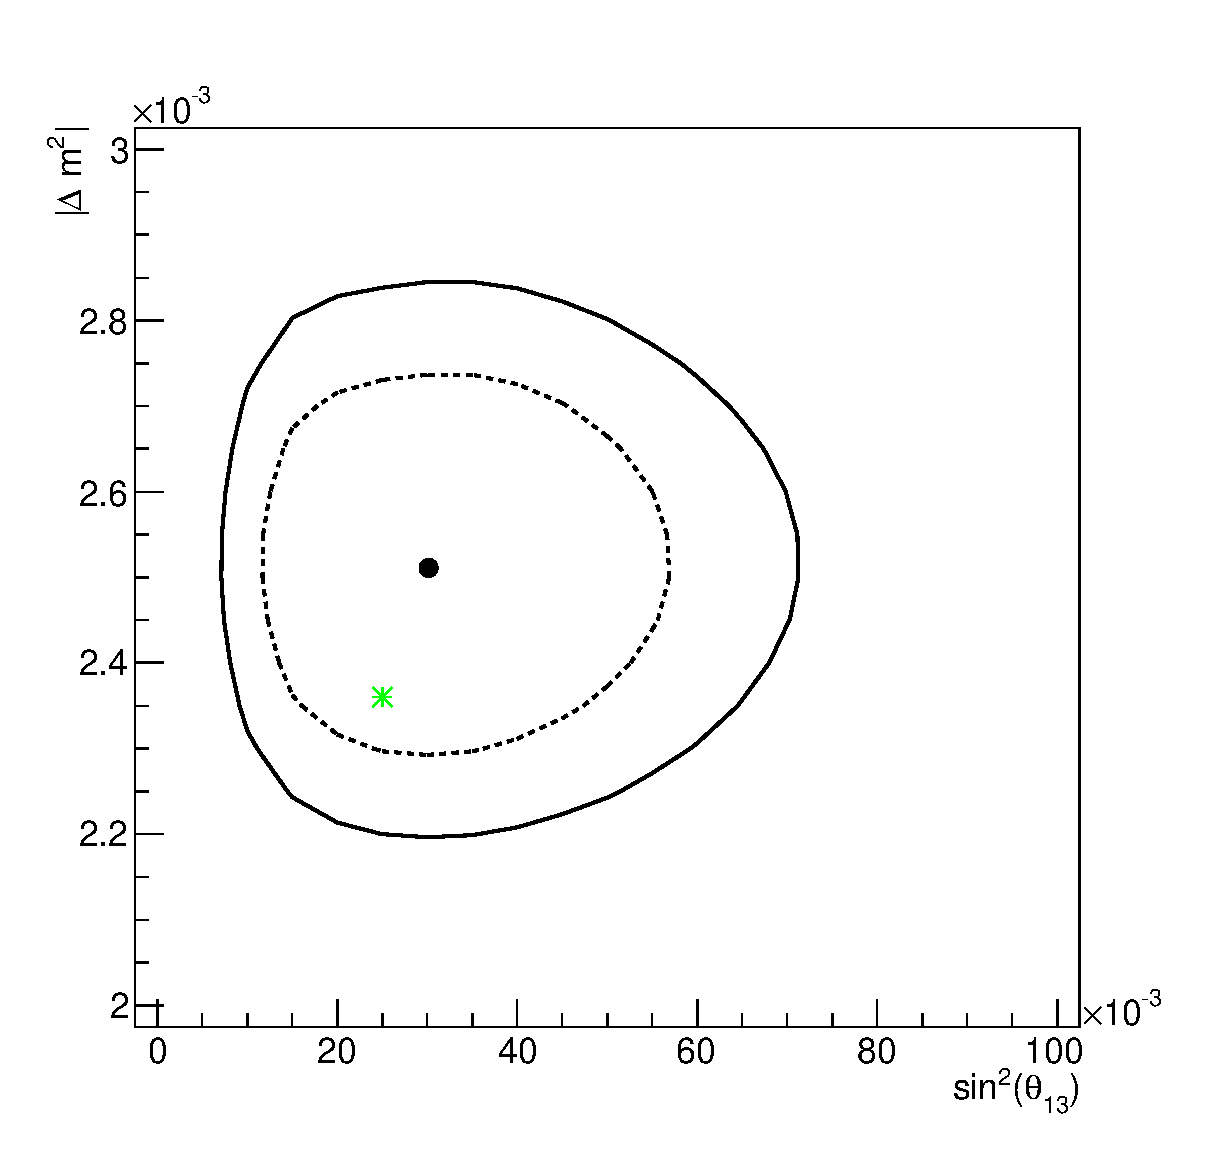
\includegraphics[width=15pc]{./images/appendix/fake_dataset_fits/realistic_fake_dataset1_chisq_theta13_dm23sq_global_min.eps}
\caption {
  68\% and 90\% CL regions in ($sin^{2}\theta_{13}$, $|\Delta m^{2}|$) space for fake dataset \#7.
  At each point, $\chi^2$ was minimized with respect to 
  all oscillation parameters not shown (and not considered to be fixed)
  and all relevant nuisance parameters.
}
\label{fig:toymc7_confreg_sinsqtheta13_Dmsq}
\end{minipage}

\vfill
\vspace*{0.7cm}

\begin{minipage}[t]{0.48\linewidth}
\center
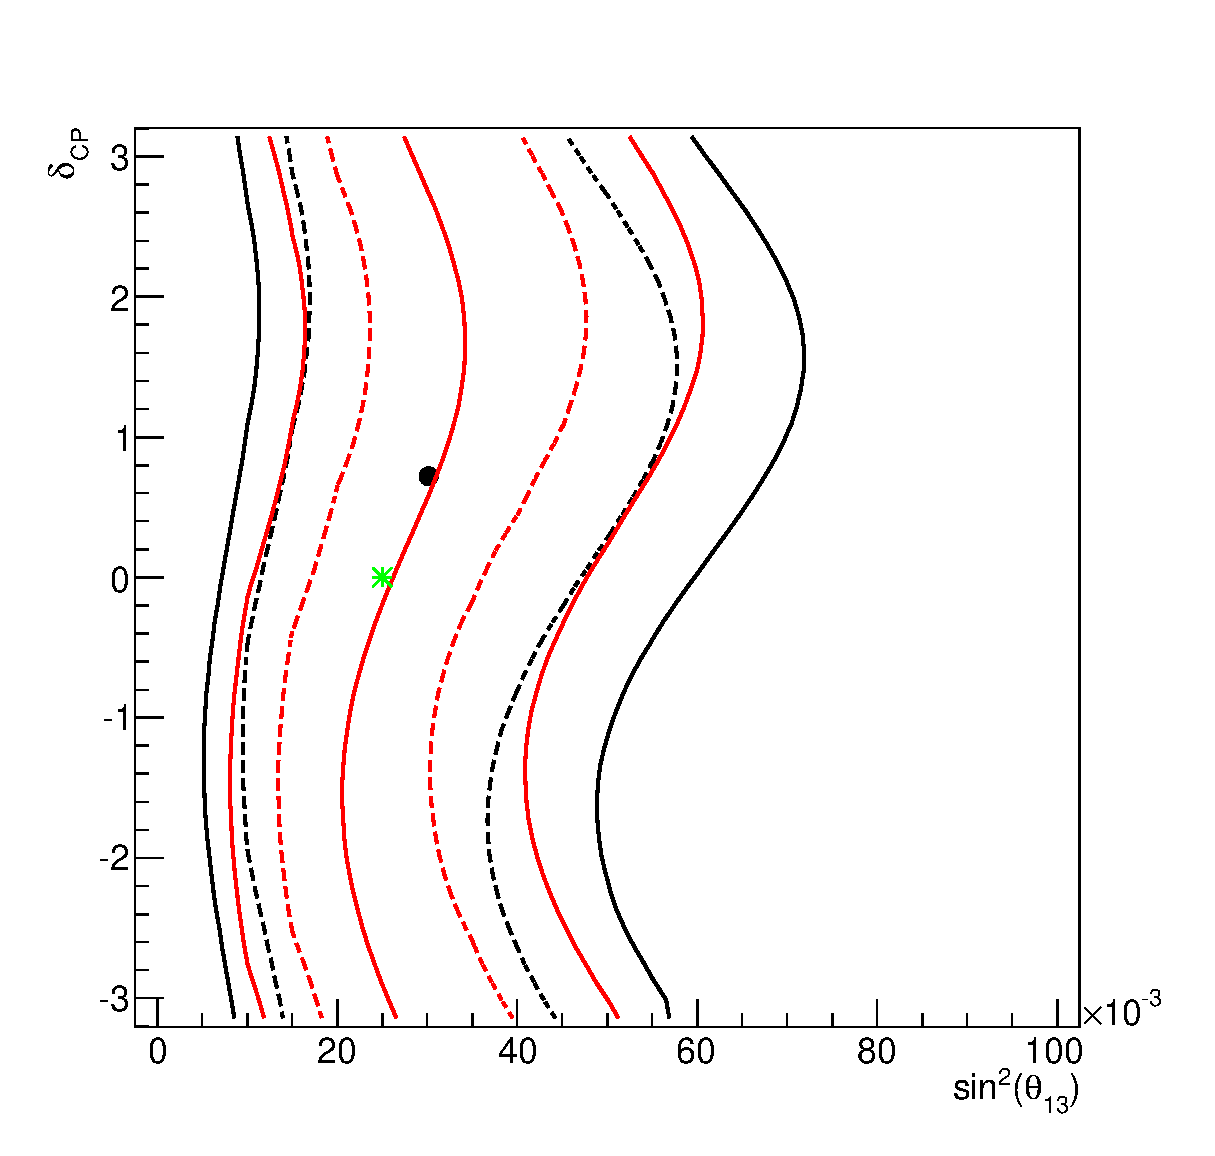
\includegraphics[width=15pc]{./images/appendix/fake_dataset_fits/realistic_fake_dataset1_chisq_theta13_deltacp_global_min.eps}
\caption {
  68\% and 90\% CL regions in ($sin^{2}\theta_{13}$, $\delta_{CP}$) space for fake dataset \#7.
  At each point, $\chi^2$ was minimized with respect to 
  $|\Delta m^{2}|$, $\sin^{2}\theta_{23}$
  and all relevant nuisance parameters for the joint analysis (black)
  and with respect to all relevant nuisance parameters for the appearance analysis (red).
  Notice that different methods are used to
  construct confidence regions for the joint analysis (global minimum) and for the 
  stand-alone appearance analysis (raster scan).
}
\label{fig:toymc7_confreg_sinsqtheta13_deltacp}
\end{minipage}
\hspace{0.03\linewidth}
\begin{minipage}[t]{0.48\linewidth}
\center
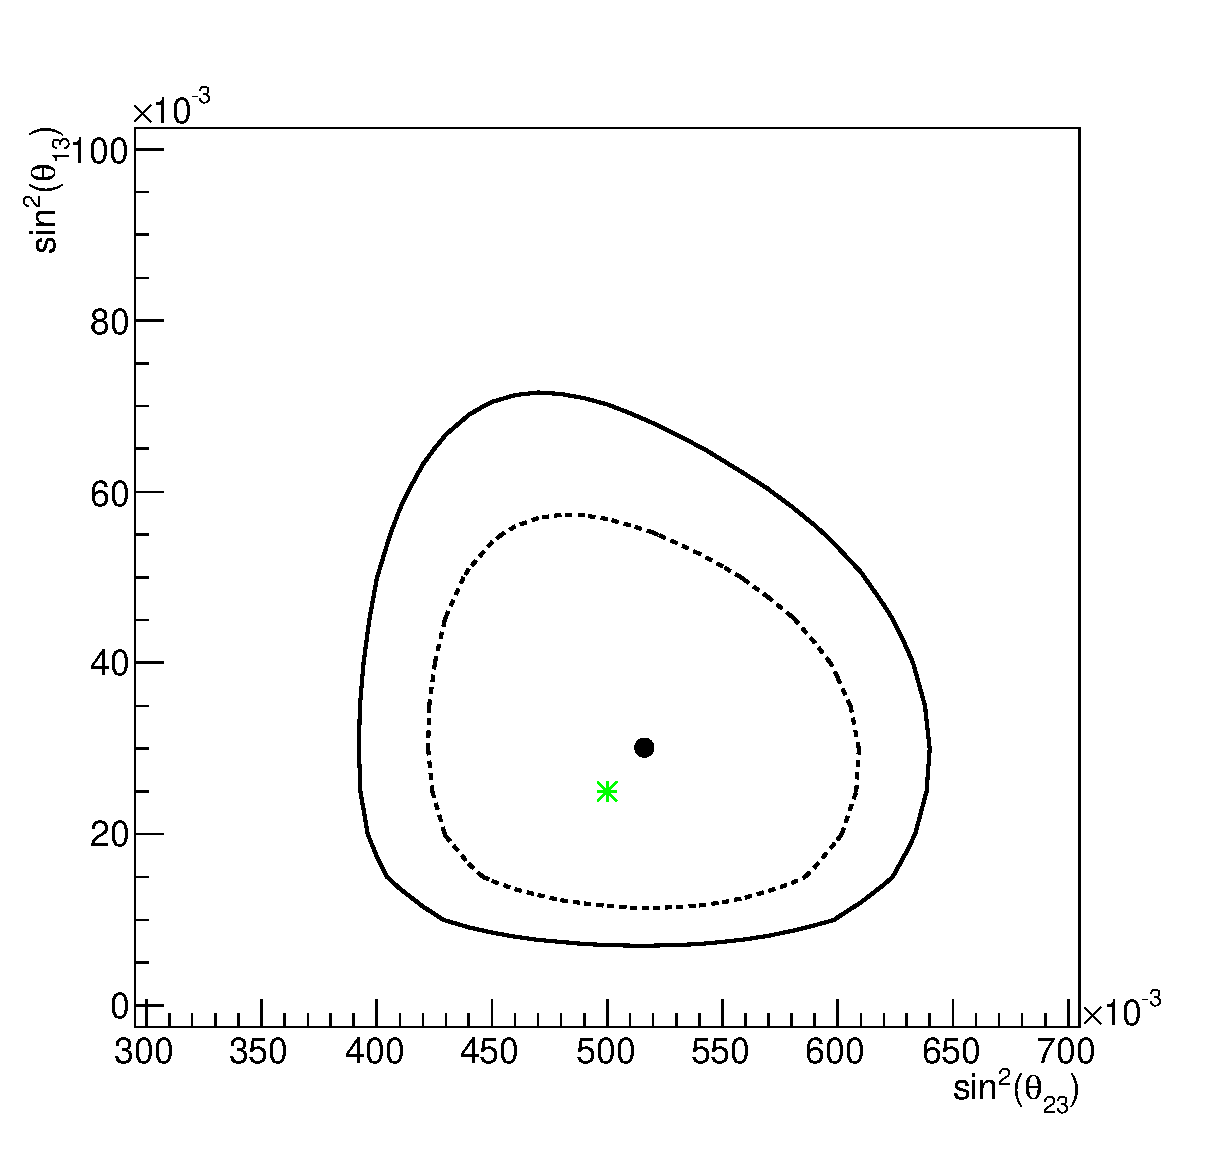
\includegraphics[width=15pc]{./images/appendix/fake_dataset_fits/realistic_fake_dataset1_chisq_theta13_theta23_global_min.eps}
\caption {
  68\% and 90\% CL regions in ($sin^{2}\theta_{23}$, $sin^{2}\theta_{13}$) space for fake dataset \#7.
  At each point, $\chi^2$ was minimized with respect to 
  all oscillation parameters not shown (and not considered to be fixed)
  and all relevant nuisance parameters.
}
\label{fig:toymc7_confreg_sinsqtheta23_sinsqtheta13}
\end{minipage}

\end{figure*}



% 
% 
% ..............................................
% Fake dataset #8
% 
%
\clearpage

\begin{figure*}[htb]

\begin{minipage}[t]{0.46\linewidth}
\center
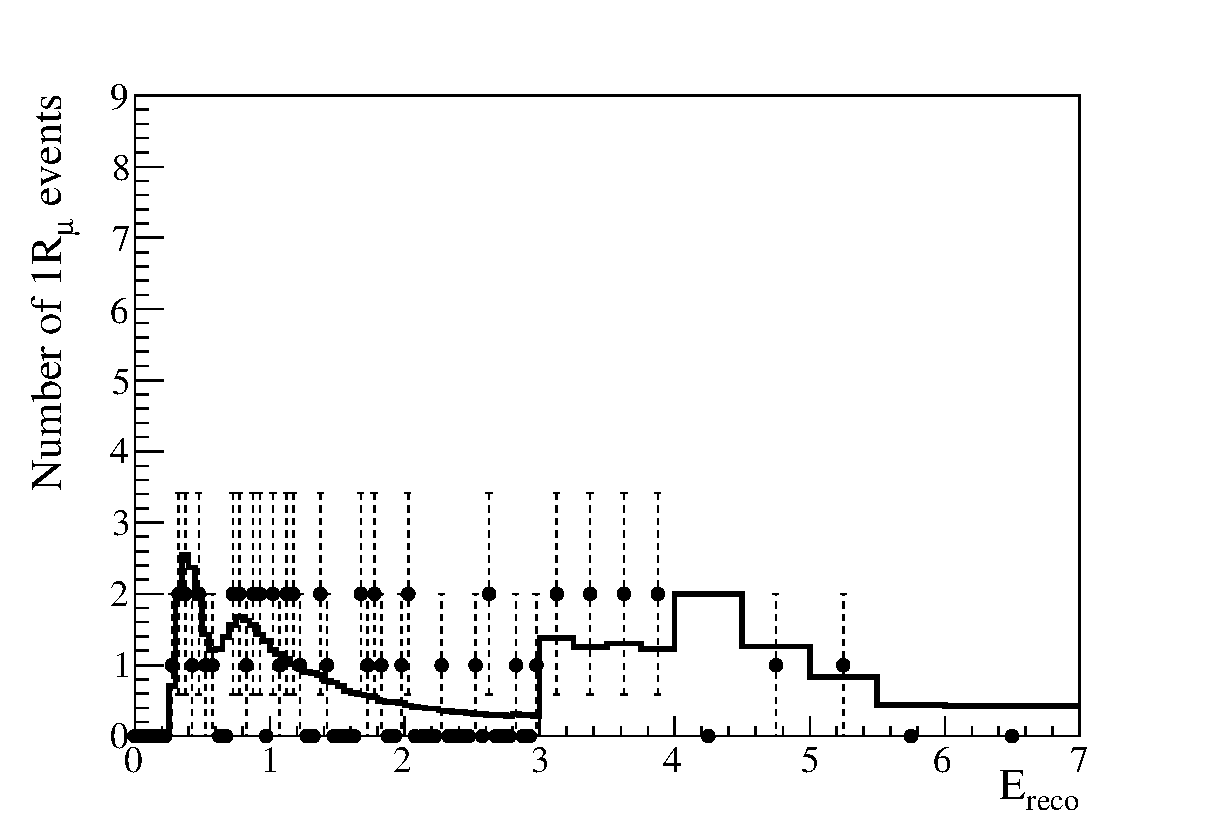
\includegraphics[width=15pc]{./images/appendix/fake_dataset_fits/realistic_fake_dataset7_nh_1st_1Rmu.eps}
\caption {
  Single $\mu$-like ring event best-fit reconstructed energy spectrum
  to fake dataset \#8.
}
\label{fig:toymc8_1Rmu_bestfit_spectrum}
\end{minipage}
\hspace{0.03\linewidth}
\begin{minipage}[t]{0.46\linewidth}
\center
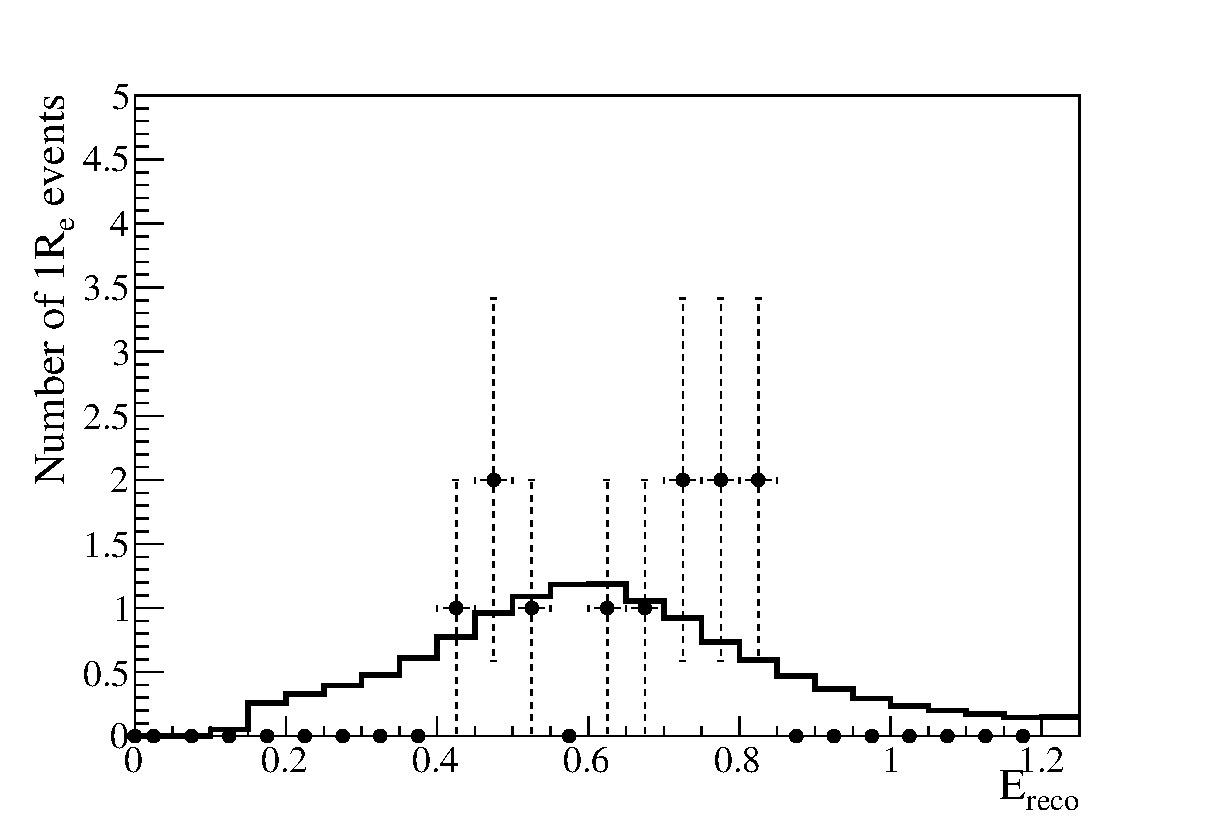
\includegraphics[width=15pc]{./images/appendix/fake_dataset_fits/realistic_fake_dataset7_nh_1st_1Re.eps}
\caption {
  Single e-like ring event best-fit reconstructed energy spectrum
  to fake dataset \#8.
}
\label{fig:toymc8_1Re_bestfit_spectrum}
\end{minipage}

\vfill
\vspace*{0.7cm}

\begin{minipage}[t]{0.90\linewidth}
\center
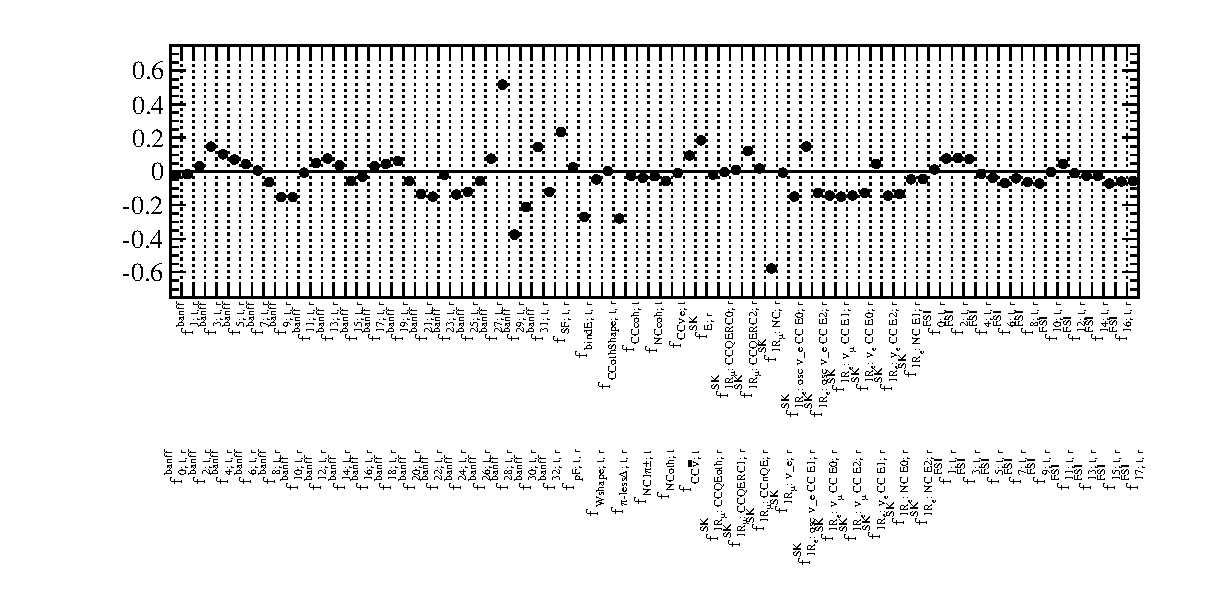
\includegraphics[width=30pc,angle=270]{./images/appendix/fake_dataset_fits/pulls_realistic_fake_dataset7_nh_1st.eps}
\caption {
  Systematic parameter pulls for the oscillation fit to fake dataset \#8.
}
\label{fig:toymc8_pulls}
\end{minipage}

\end{figure*}


%...........................................................
%
% chisq distributions used for calculating the fit p-values
%

\begin{figure*}[htb]

\begin{minipage}[t]{0.90\linewidth}
\center
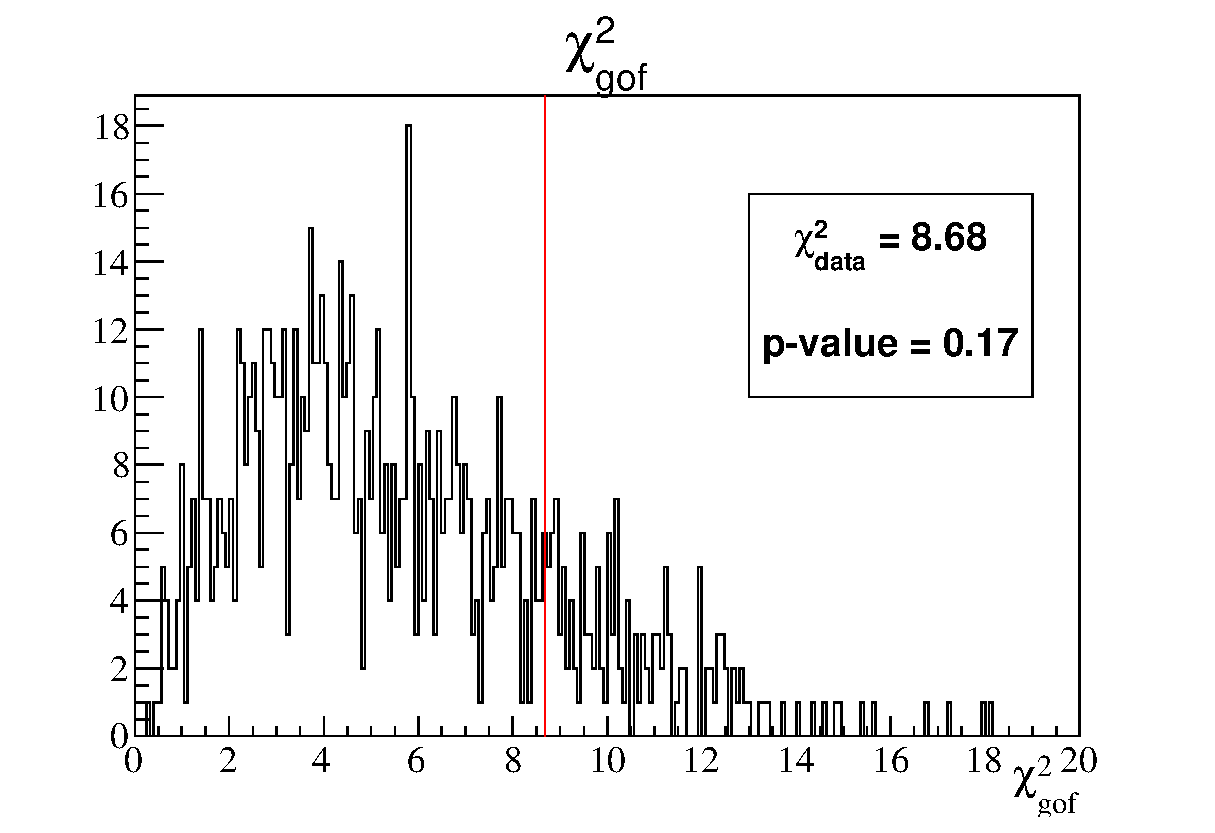
\includegraphics[width=30pc]{./images/appendix/fake_dataset_fits/realistic_fake_dataset7_nh_1st_gof_new.eps}
\caption {
  Distribution of $\chi^2_{gof}$, the goodness-of-fit (gof) $\chi^2$, 
  from 1k toy MC experiments generated at dataset \#8 joint 3-flavour analysis best-fit oscillation point.
  The $\chi^2_{gof}$ value for the dataset \#8 ($\chi^2_{data}$) is highlighted.
  All $\chi^2_{gof}$ values were computed 
  using the 5 (single $\mu$-like ring) + 3 (single e-like ring) 
  reconstructed energy binning scheme described in Sec.\ \ref{sec:goodness_of_fit}.
}
\label{fig:toymc8_gofchisq}
\end{minipage}

\vfill
\vspace*{0.7cm}

\begin{minipage}[t]{0.46\linewidth}
\center
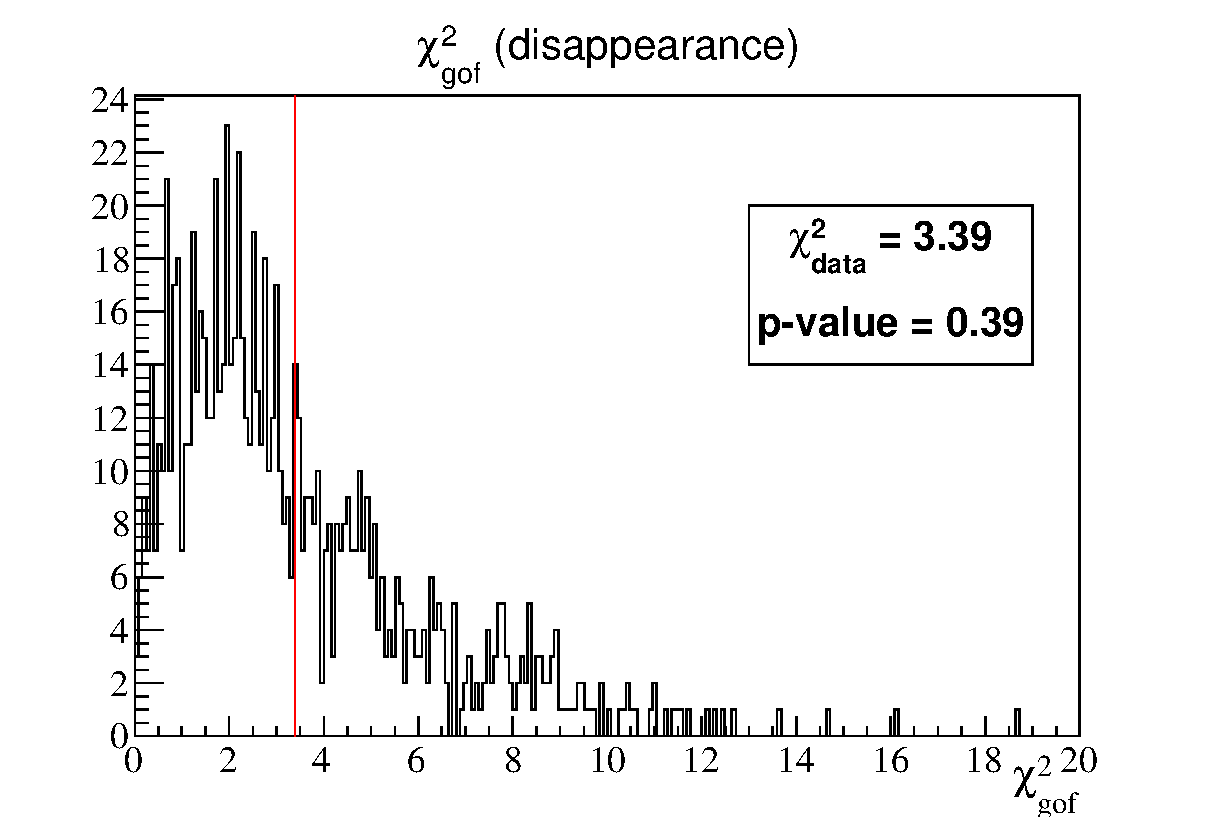
\includegraphics[width=18pc]{./images/appendix/fake_dataset_fits/realistic_fake_dataset7_nh_1st_gof_disap_new.eps}
\caption {
  Distribution of $\chi^2_{gof}$
  from 1k toy MC experiments generated at the dataset \#8 stand-alone 3-flavour $\nu_{\mu}$ disappearance analysis best-fit oscillation point.
  The $\chi^2_{gof}$ value for the dataset \#8 ($\chi^2_{data}$) is highlighted.
  All $\chi^2_{gof}$ values were computed 
  using the 5 (single $\mu$-like ring) 
  reconstructed energy binning scheme described in Sec.\ \ref{sec:goodness_of_fit}.
}
\label{fig:toymc8_gofchisq_disapp}
\end{minipage}
\hspace{0.03\linewidth}
\begin{minipage}[t]{0.46\linewidth}
\center
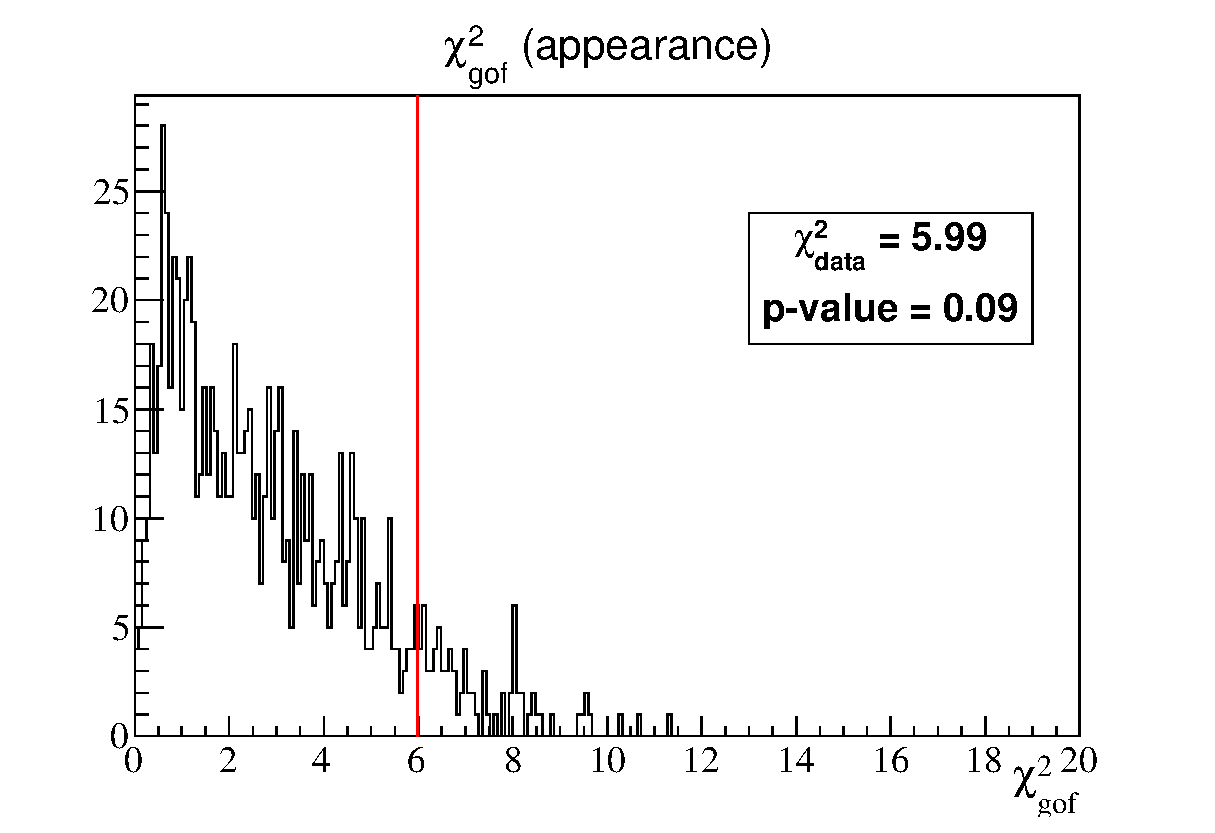
\includegraphics[width=18pc]{./images/appendix/fake_dataset_fits/realistic_fake_dataset7_nh_1st_gof_app_new.eps}
\caption {
  Distribution of $\chi^2_{gof}$
  from 1k toy MC experiments generated at the dataset \#8 stand-alone 3-flavour $\nu_{e}$ appearance analysis best-fit oscillation point.
  The $\chi^2_{gof}$ value for the dataset \#8 ($\chi^2_{data}$) is highlighted.
   All $\chi^2_{gof}$ values were computed 
  using the 3 (single e-like ring) 
  reconstructed energy binning scheme  as described in Sec.\ \ref{sec:goodness_of_fit}.
}
\label{fig:toymc8_gofchisq_app}
\end{minipage}

\end{figure*}



%
% delta\chisq and contours
%

\begin{figure*}[htb]

\begin{minipage}[t]{0.22\linewidth}
\center
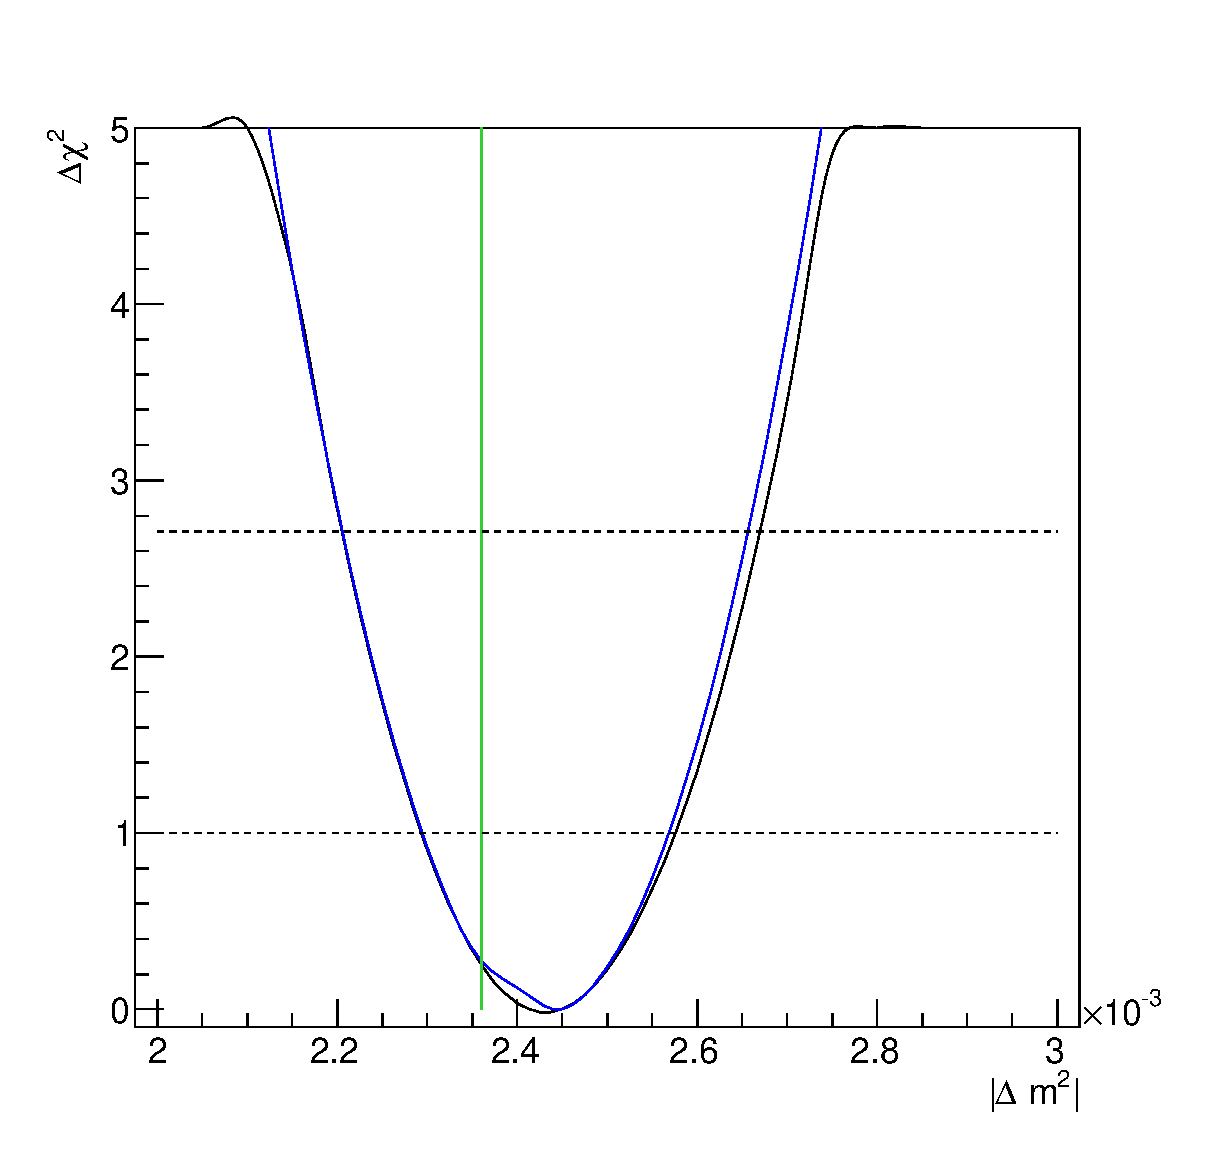
\includegraphics[width=9pc]{./images/appendix/fake_dataset_fits/realistic_fake_dataset7_chisq_dm23sq_global_min.eps}
\caption {
  $\Delta\chi^2$ as function of $|\Delta m^{2}|$ for fake dataset \#8.
  At each point, $\chi^2$ was minimized with respect to 
  $\sin^{2}\theta_{23}$, $\sin^{2}\theta_{13}$, $\delta_{CP}$
  and all relevant nuisance parameters for the joint analysis (black)
  and with respect to $\sin^{2}\theta_{23}$ and all relevant nuisance
  parameters for the disappearance analysis (blue).
}
\label{fig:toymc8_dchisq_Dmsq}
\end{minipage}
\hspace{0.02\linewidth}
\begin{minipage}[t]{0.22\linewidth}
\center
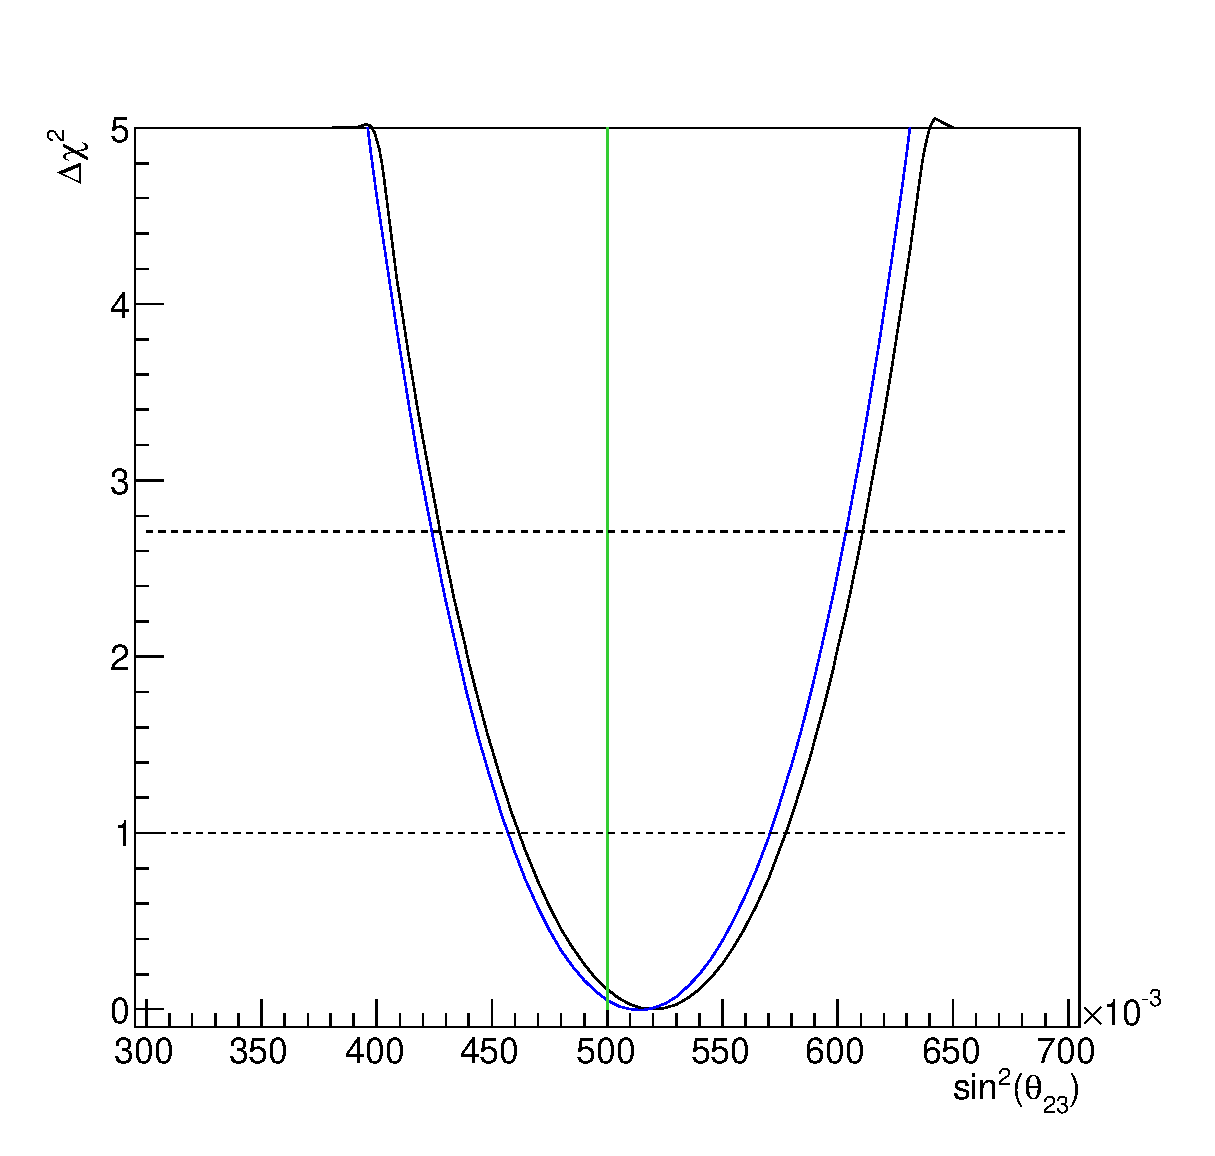
\includegraphics[width=9pc]{./images/appendix/fake_dataset_fits/realistic_fake_dataset7_chisq_theta23_global_min.eps}
\caption {
  $\Delta\chi^2$ as function of $sin^{2}\theta_{23}$ for fake dataset \#8.
  At each point, $\chi^2$ was minimized with respect to 
  $|\Delta m^{2}|$, $\sin^{2}\theta_{13}$, $\delta_{CP}$
  and all relevant nuisance parameters for the joint analysis (black)
  and with respect to $\sin^{2}\theta_{23}$ and all relevant nuisance
  parameters for the disappearance analysis (blue).
}
\label{fig:toymc8_dchisq_sinsqtheta23}
\end{minipage}
\hspace{0.02\linewidth}
\begin{minipage}[t]{0.22\linewidth}
\center
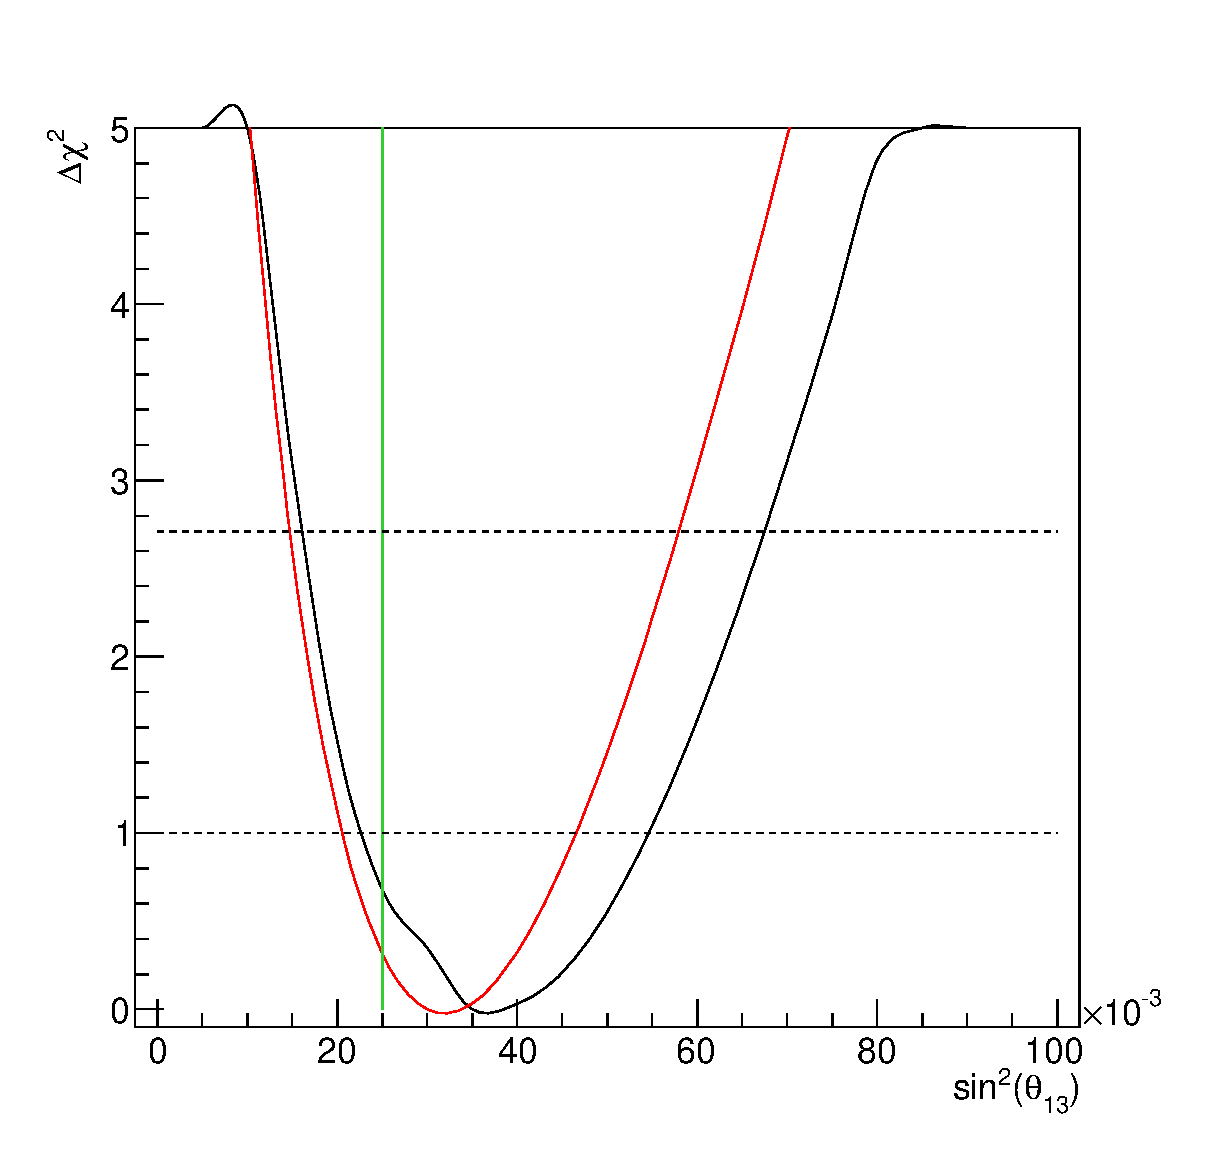
\includegraphics[width=9pc]{./images/appendix/fake_dataset_fits/realistic_fake_dataset7_chisq_theta13_global_min.eps}
\caption {
  $\Delta\chi^2$ as function of $sin^{2}\theta_{13}$ for fake dataset \#8.
  At each point, $\chi^2$ was minimized with respect to 
  $\sin^{2}\theta_{23}$, $\sin^{2}\theta_{13}$, $\delta_{CP}$
  and all relevant nuisance parameters for the joint analysis (black)
  and with respect to all relevant nuisance parameters 
  ($\delta_{CP}$ is fixed to 0) for the appearance analysis (red).
}
\label{fig:toymc8_dchisq_sinsqtheta13}
\end{minipage}
\hspace{0.02\linewidth}
\begin{minipage}[t]{0.22\linewidth}
\center
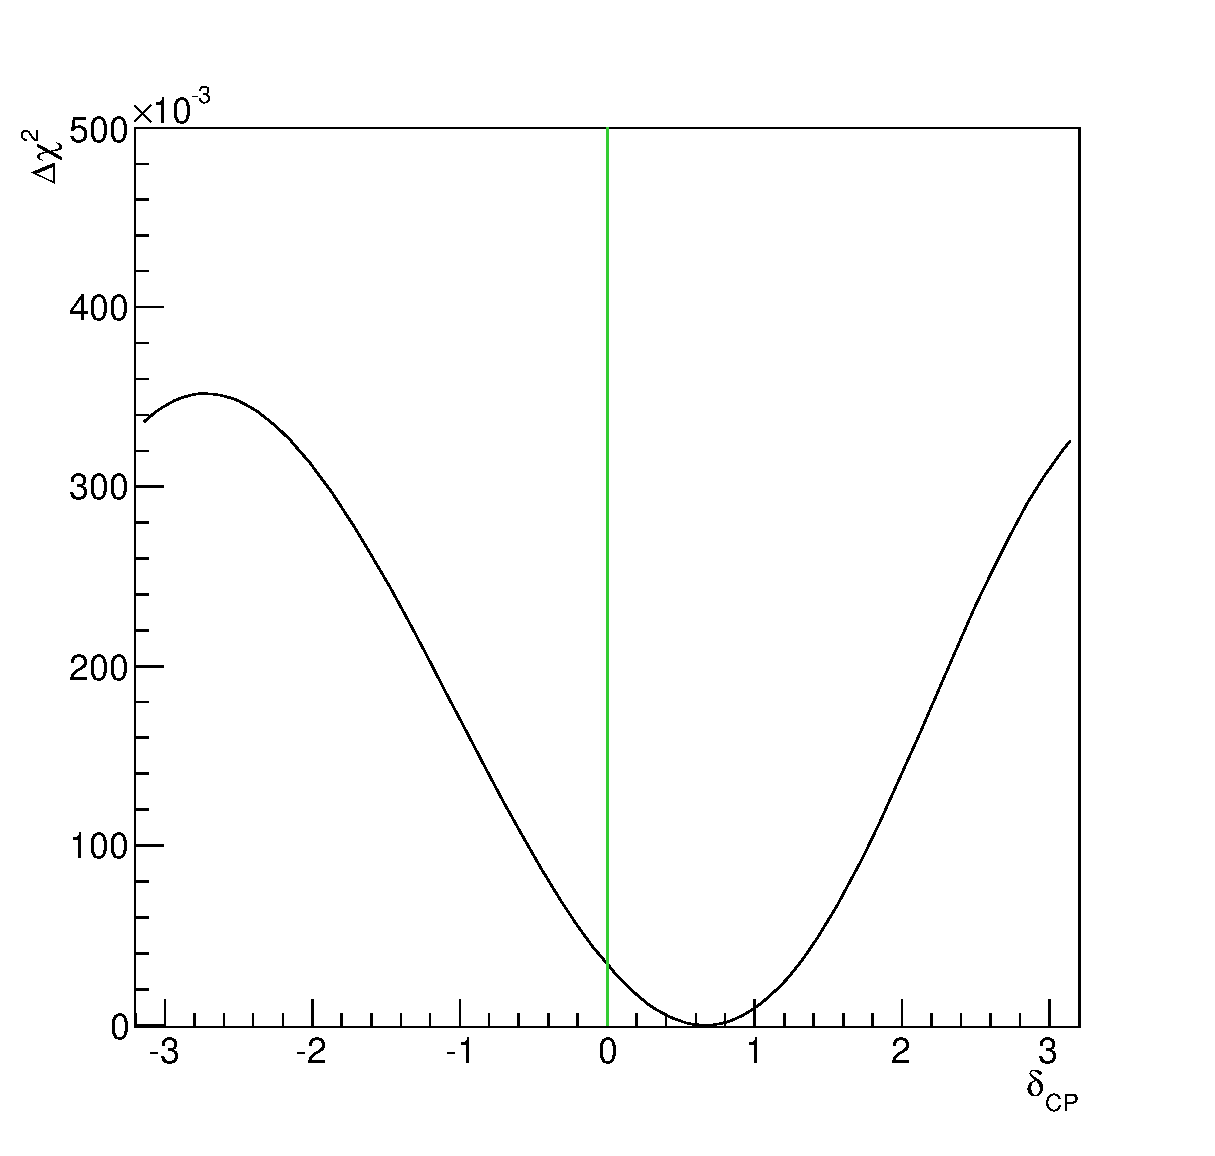
\includegraphics[width=9pc]{.//images/appendix/fake_dataset_fits/realistic_fake_dataset7_chisq_deltacp_global_min.eps}
\caption {
  $\Delta\chi^2$ as function of $\delta_{CP}$ for fake dataset \#8.
  At each point, $\chi^2$ was minimized with respect to 
  all oscillation parameters not shown (and not considered to be fixed)
  and all relevant nuisance parameters.
}
\label{fig:toymc8_dchisq_deltacp}
\end{minipage}
\vfill
\vspace*{0.7cm}
\begin{minipage}[t]{0.48\linewidth}
\center
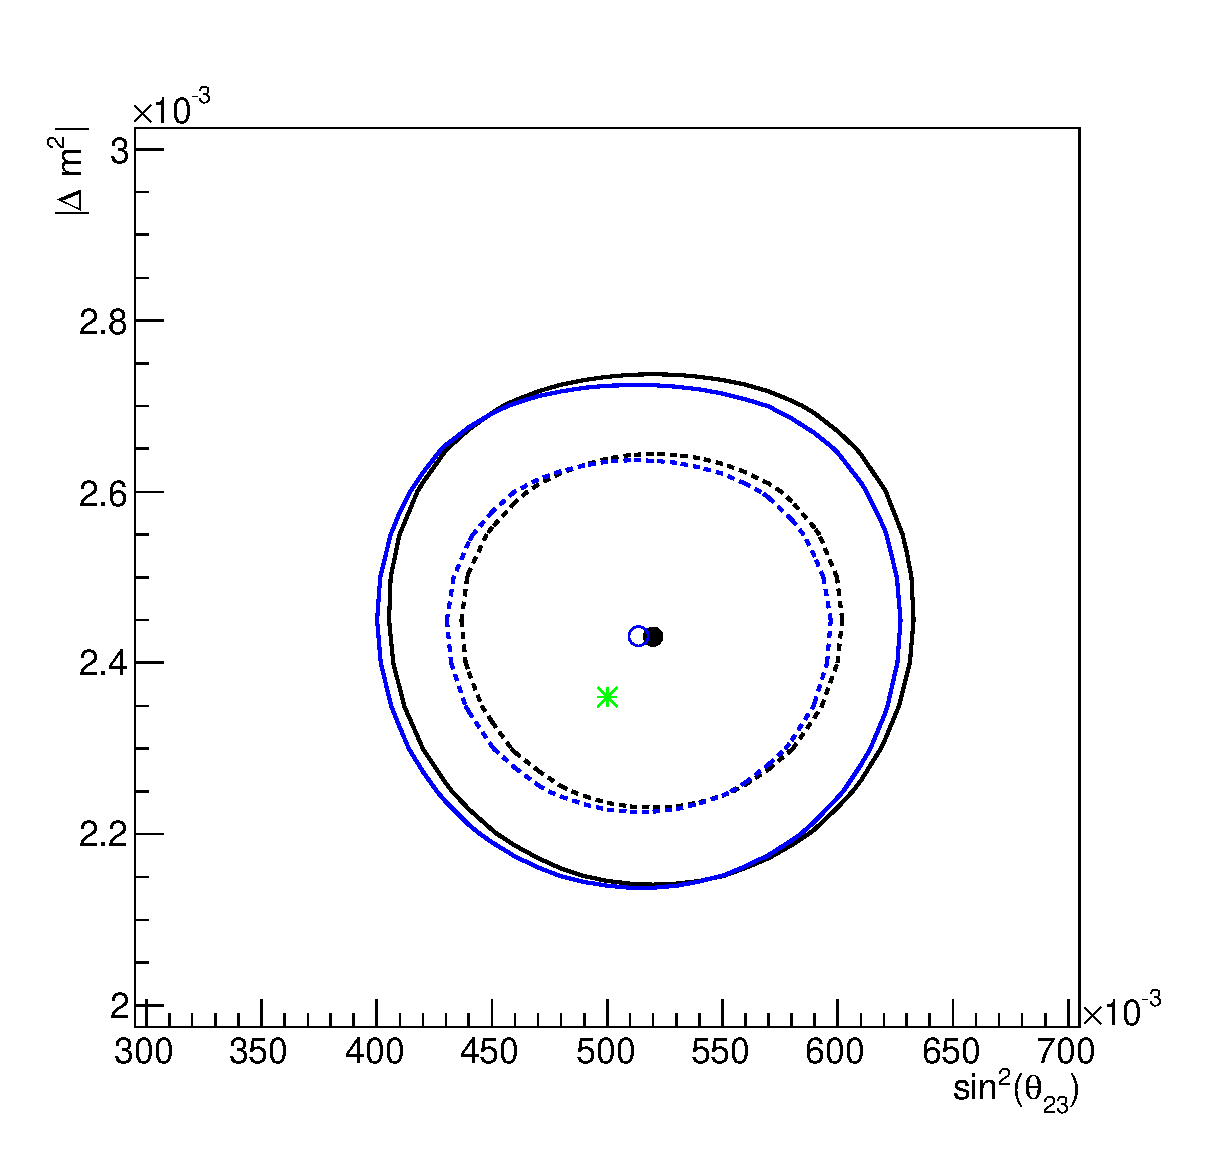
\includegraphics[width=15pc]{./images/appendix/fake_dataset_fits/realistic_fake_dataset7_chisq_theta23_dm23sq_global_min.eps}
\caption {
  68\% and 90\% CL regions in ($sin^{2}\theta_{23}$, $|\Delta m^{2}|$) space for fake dataset \#8.
  At each point, $\chi^2$ was minimized with respect to 
  $\sin^{2}\theta_{13}$, $\delta_{CP}$
  and all relevant nuisance parameters for the joint analysis (black)
  and with respect to all relevant nuisance parameters for the disappearance analysis (blue).
}
\label{fig:toymc8_confreg_sinsqtheta23_Dmsq}
\end{minipage}
\hspace{0.03\linewidth}
\begin{minipage}[t]{0.48\linewidth}
\center
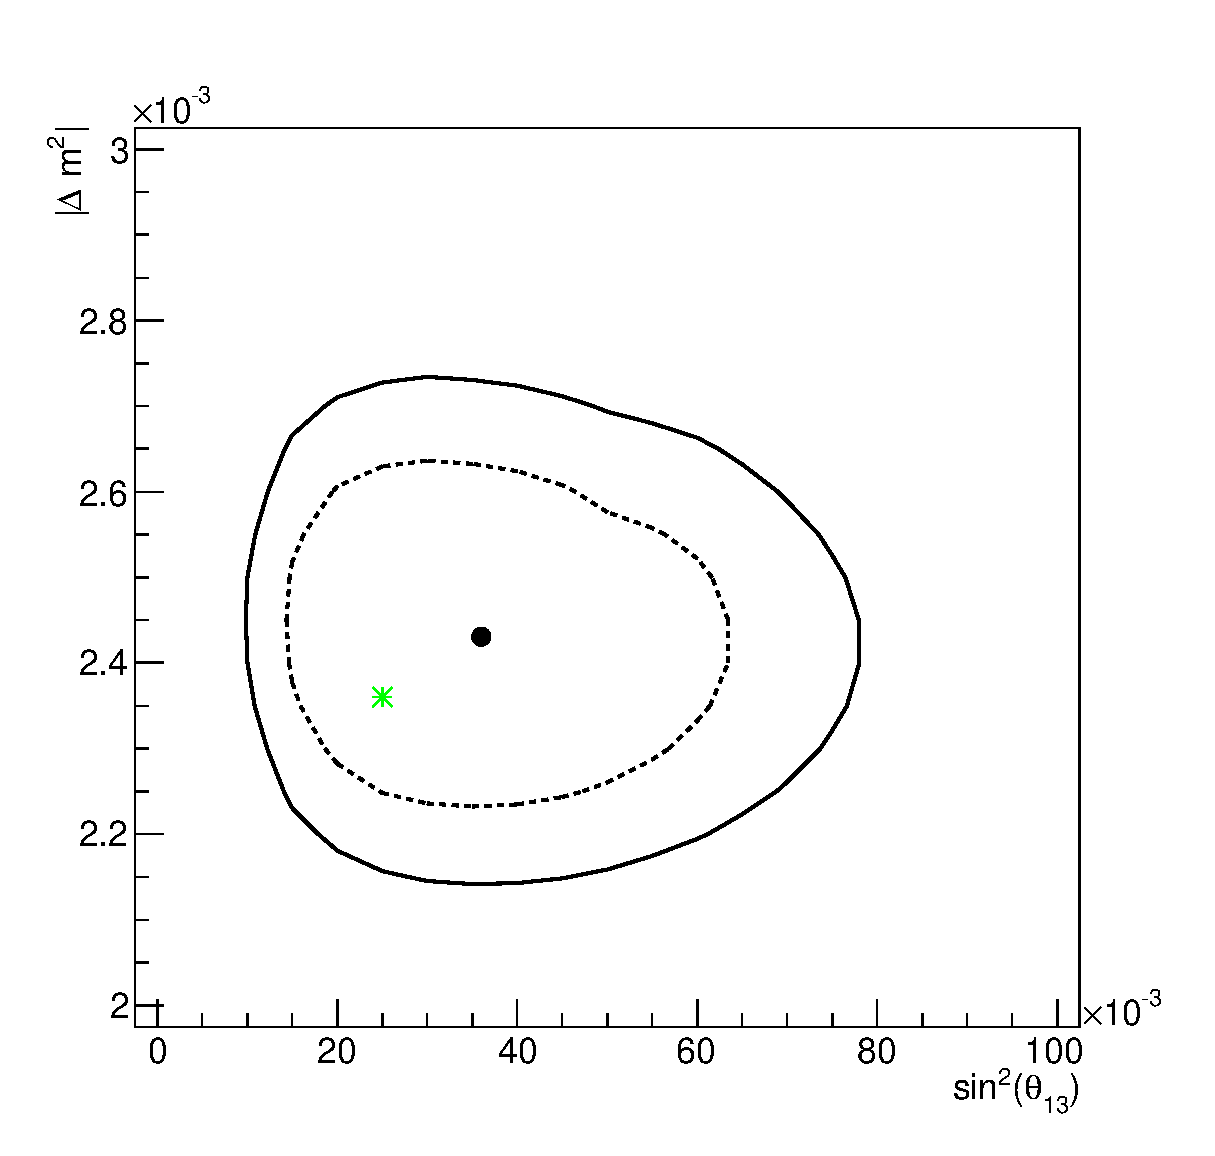
\includegraphics[width=15pc]{./images/appendix/fake_dataset_fits/realistic_fake_dataset7_chisq_theta13_dm23sq_global_min.eps}
\caption {
  68\% and 90\% CL regions in ($sin^{2}\theta_{13}$, $|\Delta m^{2}|$) space for fake dataset \#8.
  At each point, $\chi^2$ was minimized with respect to 
  all oscillation parameters not shown (and not considered to be fixed)
  and all relevant nuisance parameters.
}
\label{fig:toymc8_confreg_sinsqtheta13_Dmsq}
\end{minipage}

\vfill
\vspace*{0.7cm}

\begin{minipage}[t]{0.48\linewidth}
\center
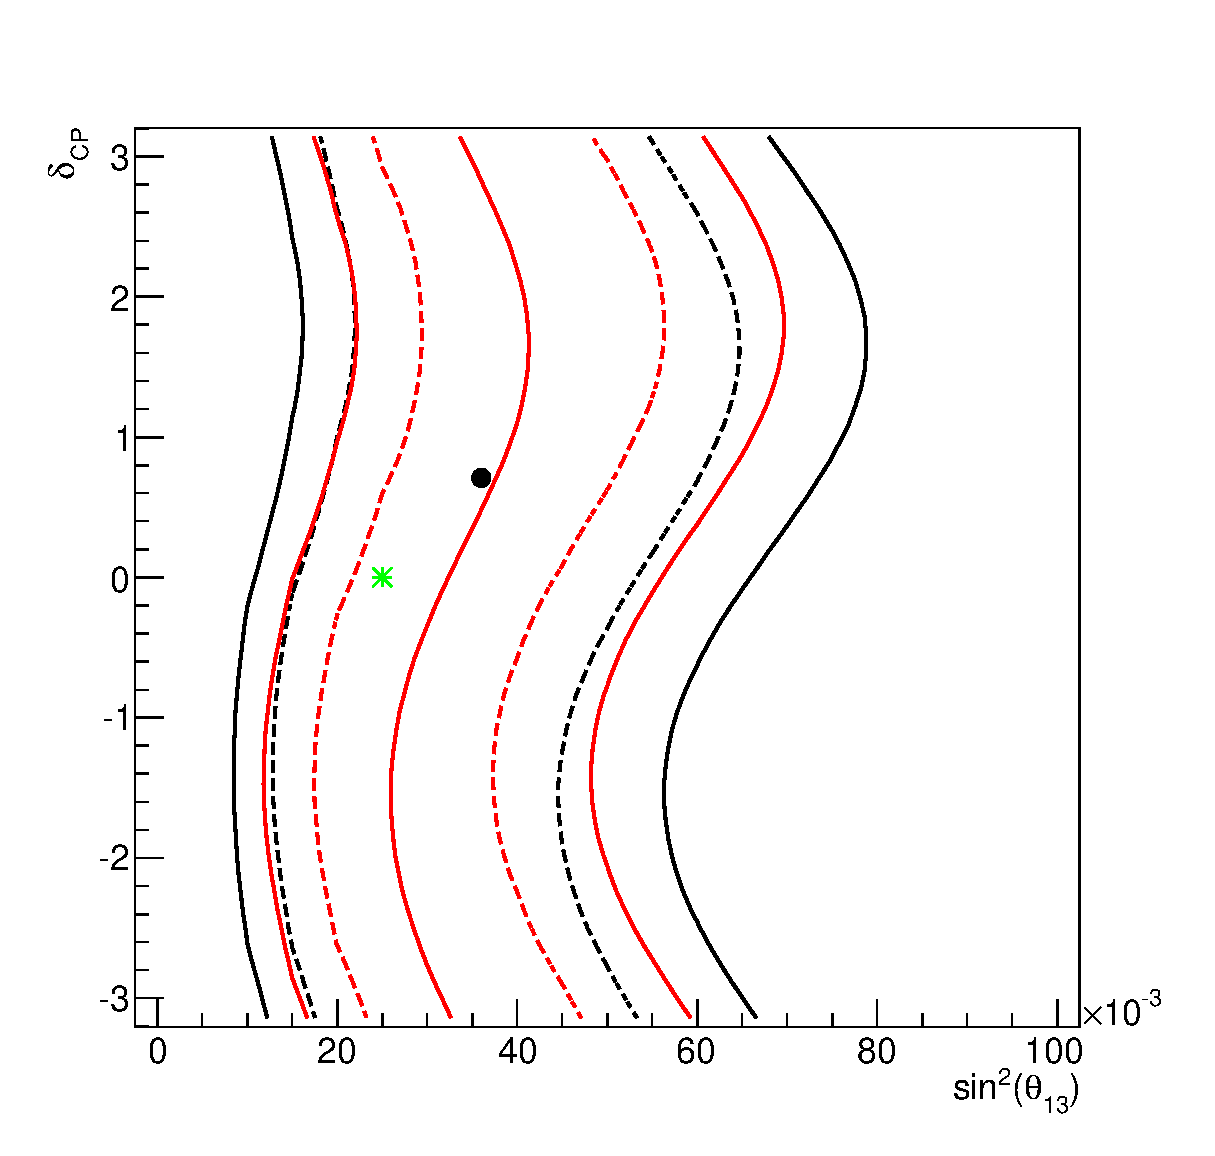
\includegraphics[width=15pc]{./images/appendix/fake_dataset_fits/realistic_fake_dataset7_chisq_theta13_deltacp_global_min.eps}
\caption {
  68\% and 90\% CL regions in ($sin^{2}\theta_{13}$, $\delta_{CP}$) space for fake dataset \#8.
  At each point, $\chi^2$ was minimized with respect to 
  $|\Delta m^{2}|$, $\sin^{2}\theta_{23}$
  and all relevant nuisance parameters for the joint analysis (black)
  and with respect to all relevant nuisance parameters for the appearance analysis (red).
  Notice that different methods are used to
  construct confidence regions for the joint analysis (global minimum) and for the 
  stand-alone appearance analysis (raster scan).
}
\label{fig:toymc8_confreg_sinsqtheta13_deltacp}
\end{minipage}
\hspace{0.03\linewidth}
\begin{minipage}[t]{0.48\linewidth}
\center
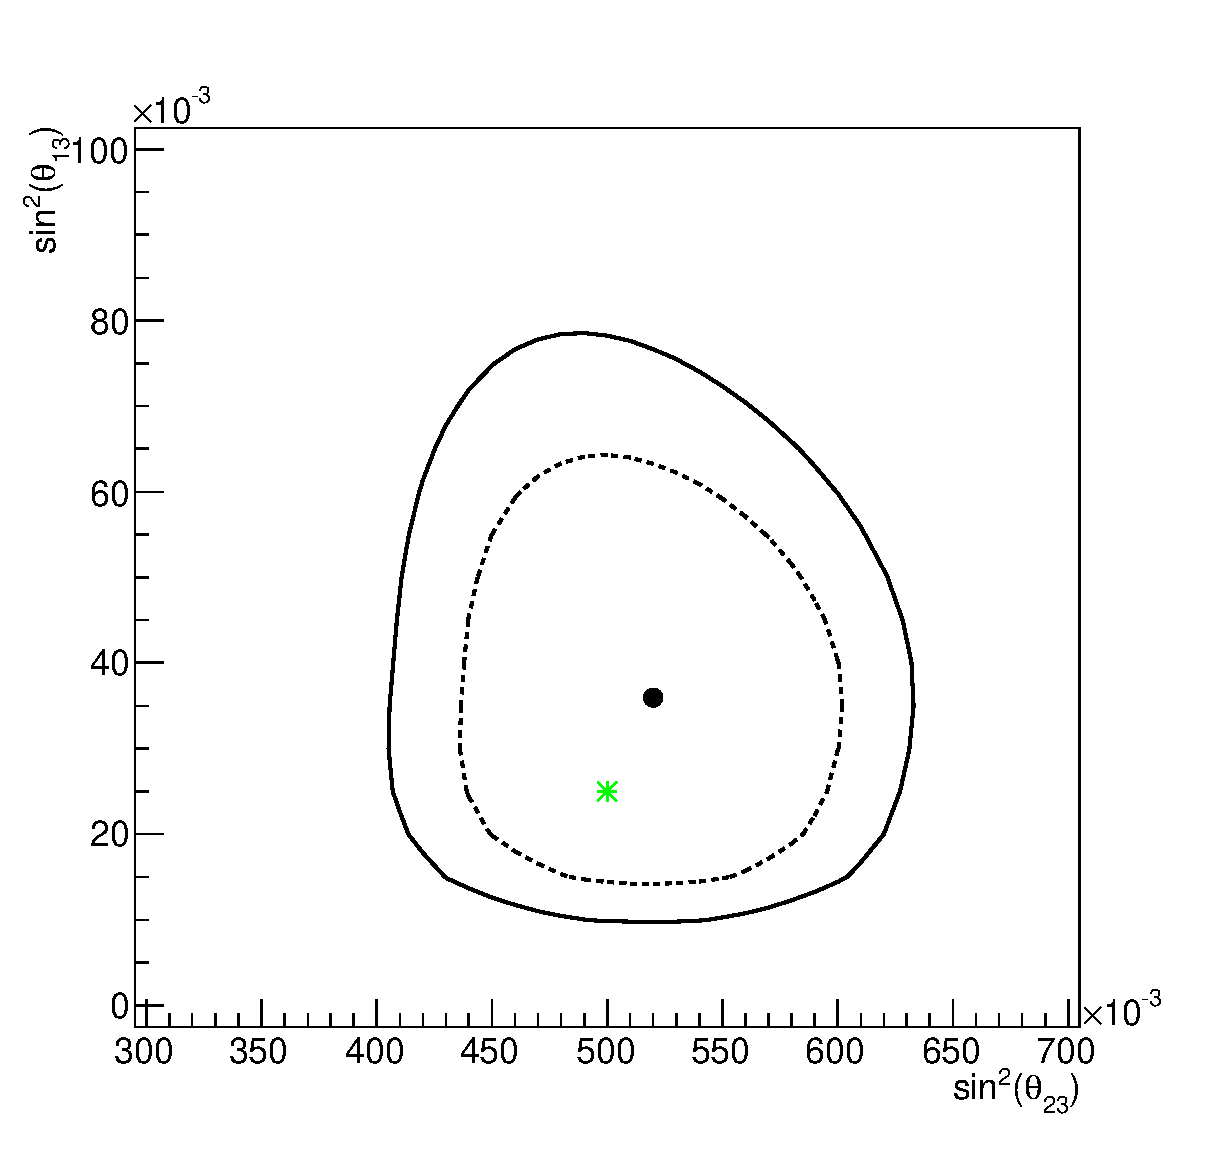
\includegraphics[width=15pc]{./images/appendix/fake_dataset_fits/realistic_fake_dataset7_chisq_theta13_theta23_global_min.eps}
\caption {
  68\% and 90\% CL regions in ($sin^{2}\theta_{23}$, $sin^{2}\theta_{13}$) space for fake dataset \#8.
  At each point, $\chi^2$ was minimized with respect to 
  all oscillation parameters not shown (and not considered to be fixed)
  and all relevant nuisance parameters.
}
\label{fig:toymc8_confreg_sinsqtheta23_sinsqtheta13}
\end{minipage}

\end{figure*}




% 
% 
% ..............................................
% Fake dataset #9
% 
%

\clearpage
\begin{figure*}[htb]

\begin{minipage}[t]{0.46\linewidth}
\center
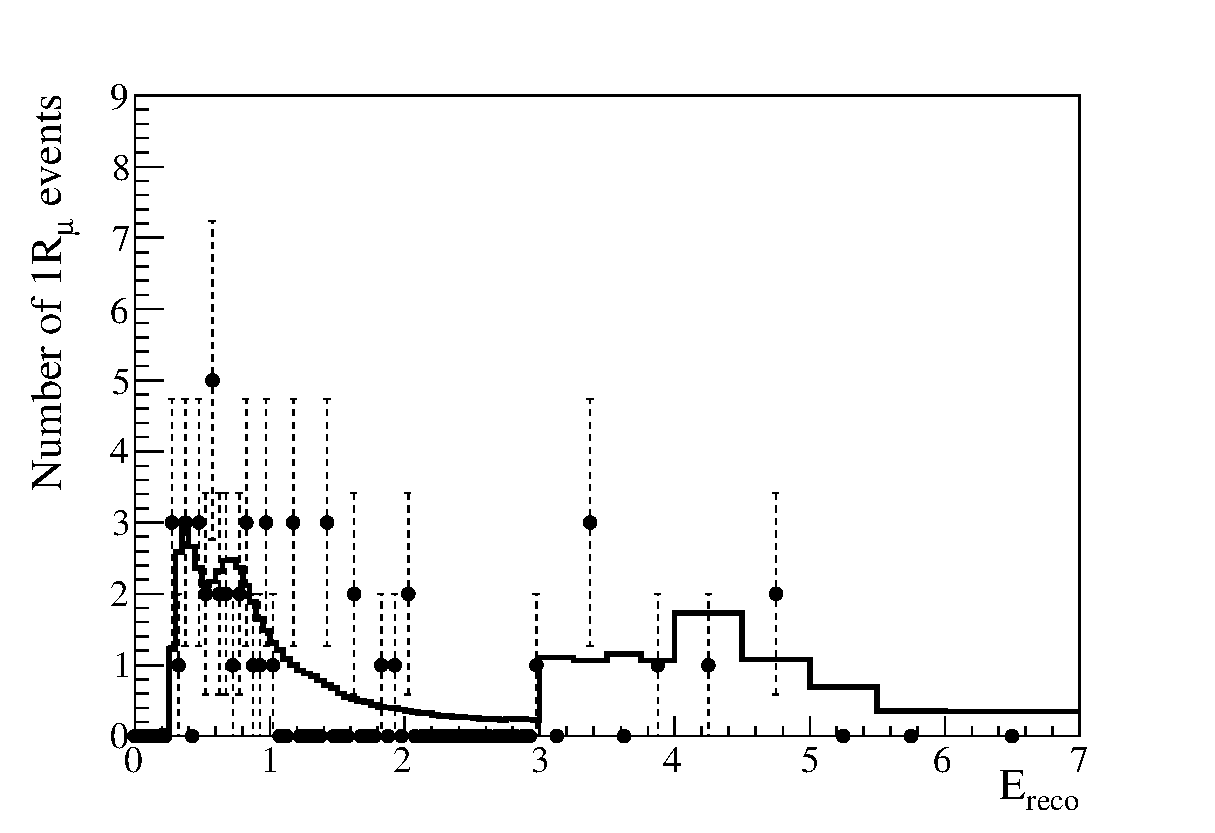
\includegraphics[width=15pc]{./images/appendix/fake_dataset_fits/realistic_fake_dataset2_nh_1st_1Rmu.eps}
\caption {
  Single $\mu$-like ring event best-fit reconstructed energy spectrum
  to fake dataset \#9.
}
\label{fig:toymc9_1Rmu_bestfit_spectrum}
\end{minipage}
\hspace{0.03\linewidth}
\begin{minipage}[t]{0.46\linewidth}
\center
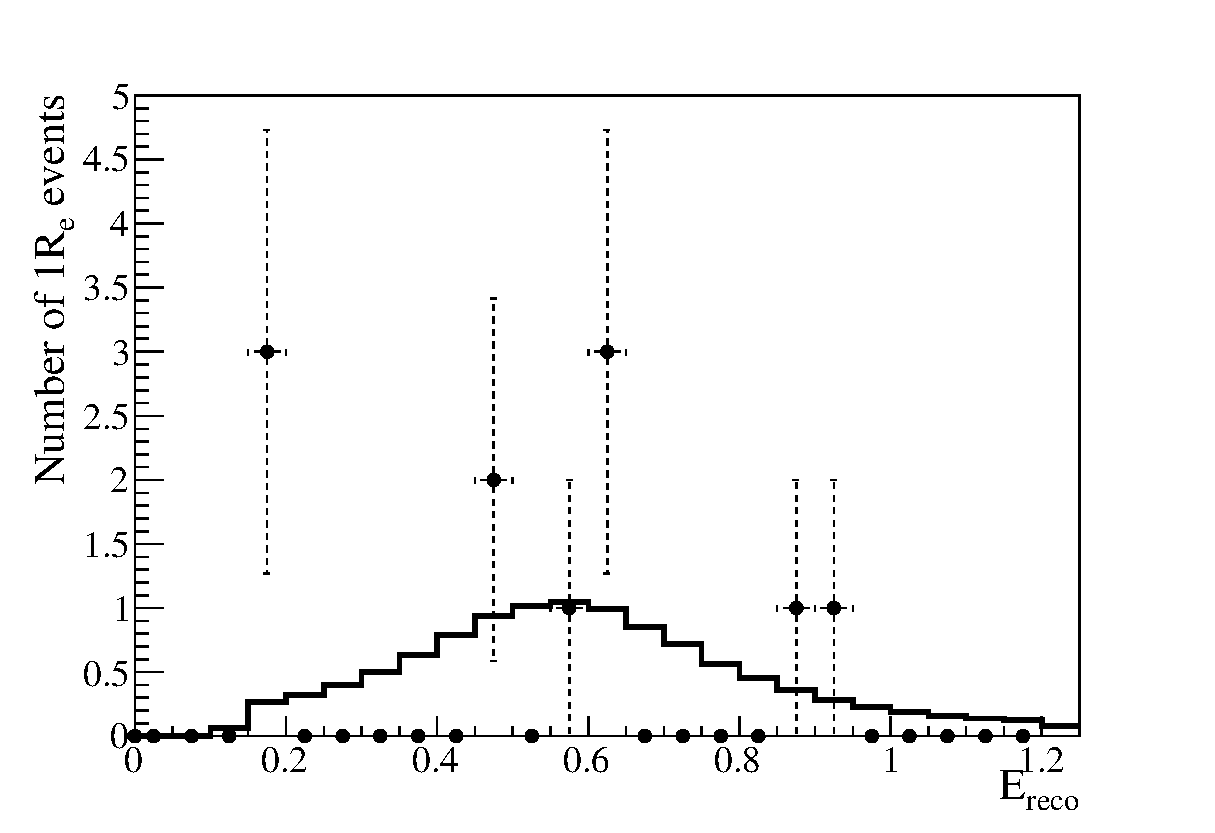
\includegraphics[width=15pc]{./images/appendix/fake_dataset_fits/realistic_fake_dataset2_nh_1st_1Re.eps}
\caption {
  Single e-like ring event best-fit reconstructed energy spectrum
  to fake dataset \#9.
}
\label{fig:toymc9_1Re_bestfit_spectrum}
\end{minipage}

\vfill
\vspace*{0.7cm}

\begin{minipage}[t]{0.90\linewidth}
\center
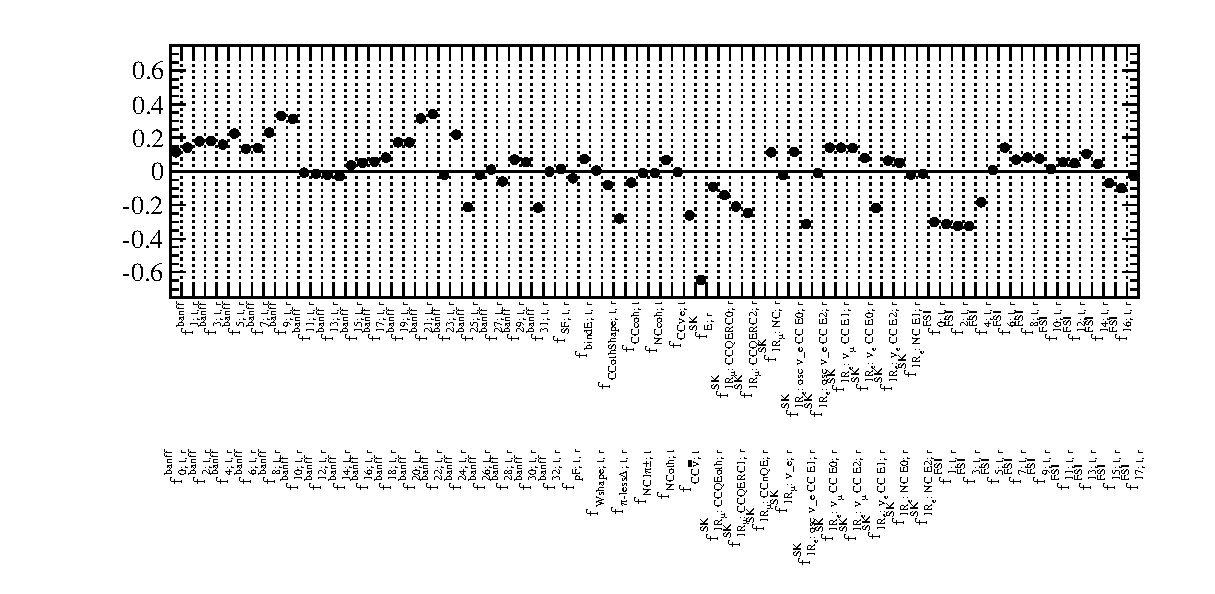
\includegraphics[width=30pc,angle=270]{./images/appendix/fake_dataset_fits/pulls_realistic_fake_dataset2_nh_1st.eps}
\caption {
  Systematic parameter pulls for the oscillation fit to fake dataset \#9.
}
\label{fig:toymc9_pulls}
\end{minipage}

\end{figure*}


%...........................................................
%
% chisq distributions used for calculating the fit p-values
%

\begin{figure*}[htb]

\begin{minipage}[t]{0.90\linewidth}
\center
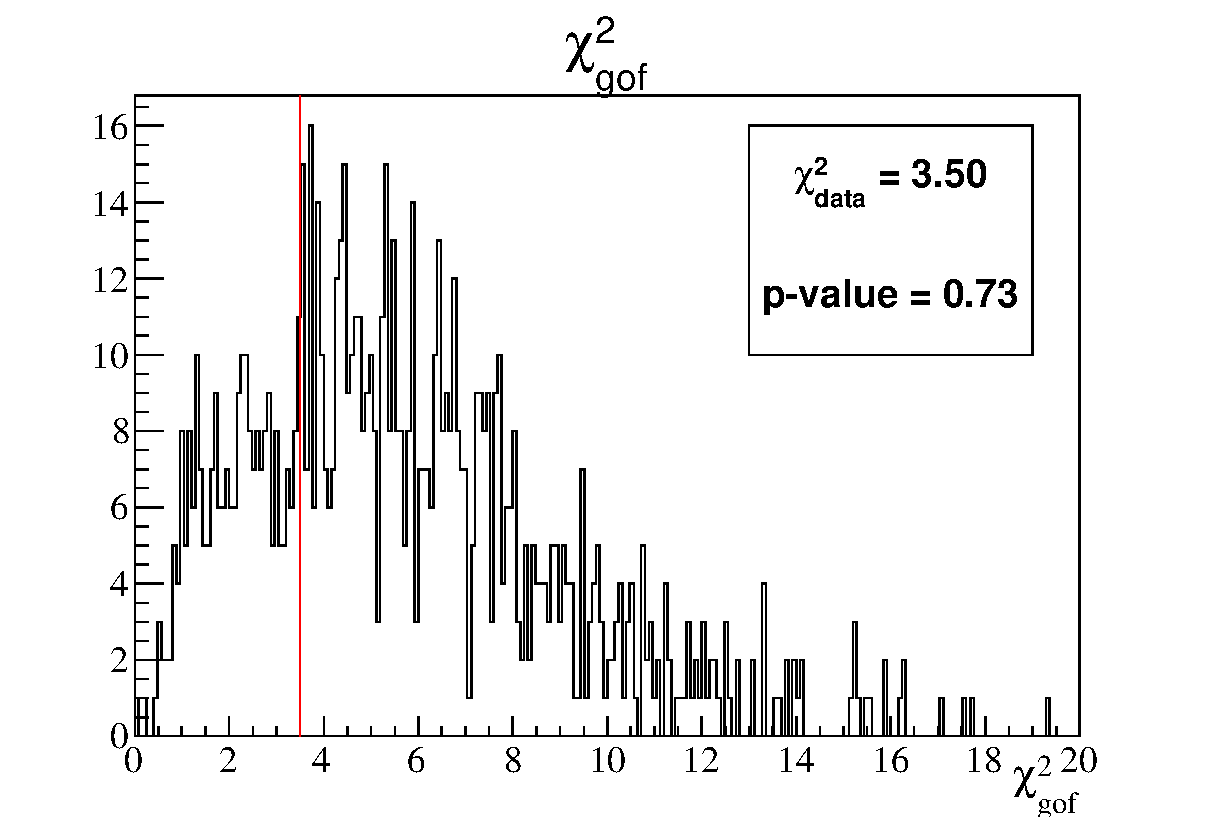
\includegraphics[width=30pc]{./images/appendix/fake_dataset_fits/realistic_fake_dataset2_nh_1st_gof_new.eps}
\caption {
  Distribution of $\chi^2_{gof}$, the goodness-of-fit (gof) $\chi^2$, 
  from 1k toy MC experiments generated at dataset \#9 joint 3-flavour analysis best-fit oscillation point.
  The $\chi^2_{gof}$ value for the dataset \#9 ($\chi^2_{data}$) is highlighted.
  All $\chi^2_{gof}$ values were computed 
  using the 5 (single $\mu$-like ring) + 3 (single e-like ring) 
  reconstructed energy binning scheme described in Sec.\ \ref{sec:goodness_of_fit}.
}
\label{fig:toymc9_gofchisq}
\end{minipage}

\vfill
\vspace*{0.7cm}

\begin{minipage}[t]{0.46\linewidth}
\center
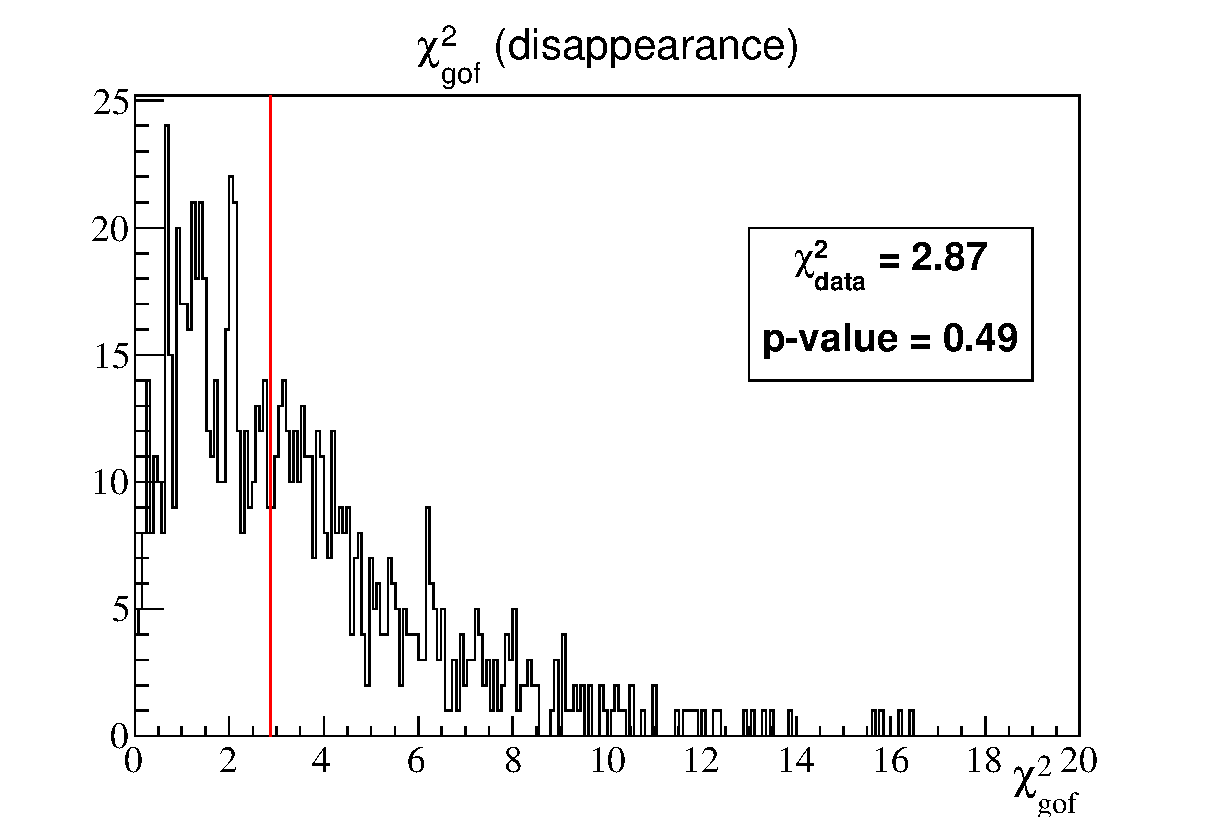
\includegraphics[width=18pc]{./images/appendix/fake_dataset_fits/realistic_fake_dataset2_nh_1st_gof_disap_new.eps}
\caption {
  Distribution of $\chi^2_{gof}$
  from 1k toy MC experiments generated at the dataset \#9 stand-alone 3-flavour $\nu_{\mu}$ disappearance analysis best-fit oscillation point.
  The $\chi^2_{gof}$ value for the dataset \#9 ($\chi^2_{data}$) is highlighted.
  All $\chi^2_{gof}$ values were computed 
  using the 5 (single $\mu$-like ring) 
  reconstructed energy binning scheme described in Sec.\ \ref{sec:goodness_of_fit}.
}
\label{fig:toymc9_gofchisq_disapp}
\end{minipage}
\hspace{0.03\linewidth}
\begin{minipage}[t]{0.46\linewidth}
\center
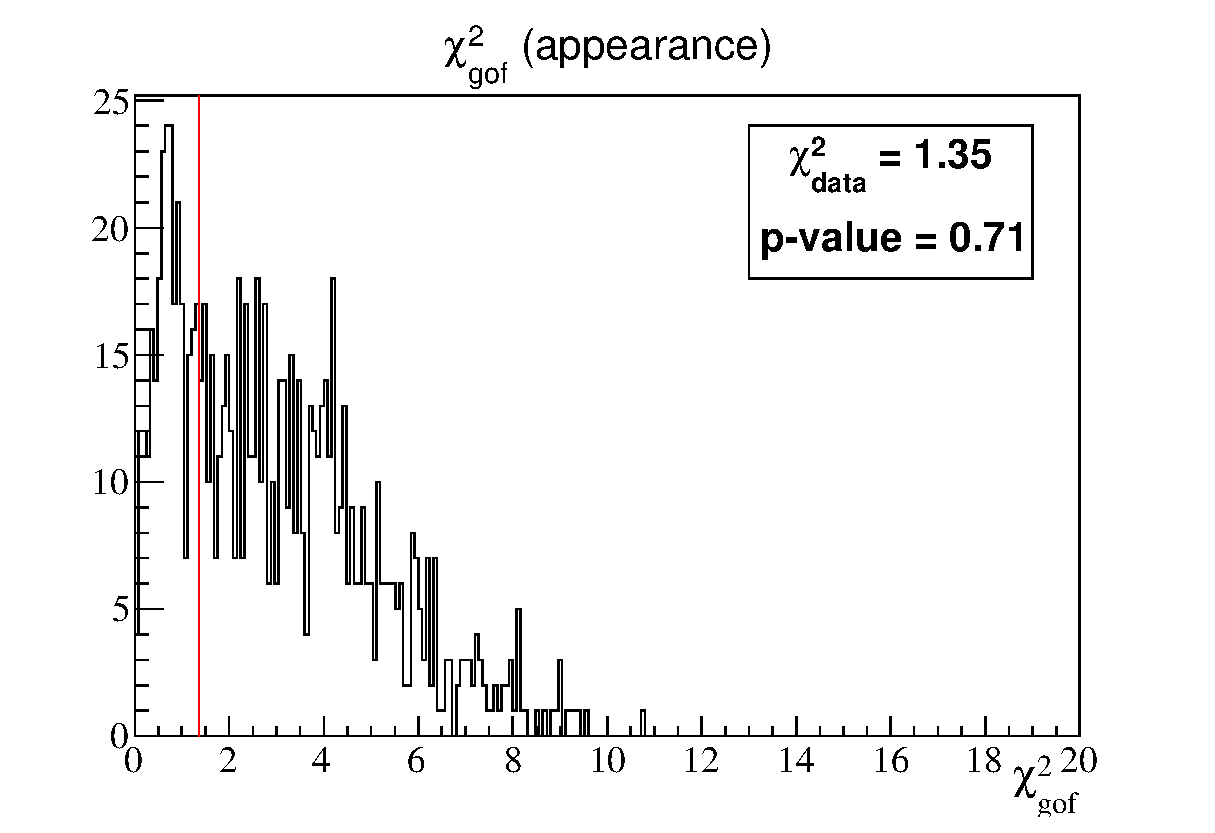
\includegraphics[width=18pc]{./images/appendix/fake_dataset_fits/realistic_fake_dataset2_nh_1st_gof_app_new.eps}
\caption {
  Distribution of $\chi^2_{gof}$
  from 1k toy MC experiments generated at the dataset \#9 stand-alone 3-flavour $\nu_{e}$ appearance analysis best-fit oscillation point.
  The $\chi^2_{gof}$ value for the dataset \#9 ($\chi^2_{data}$) is highlighted.
  All $\chi^2_{gof}$ values were computed 
  using the 3 (single e-like ring) 
  reconstructed energy binning scheme  as described in Sec.\ \ref{sec:goodness_of_fit}.
  }
\label{fig:toymc9_gofchisq_app}
\end{minipage}

\end{figure*}



%
% delta\chisq and contours
%

\begin{figure*}[htb]

\begin{minipage}[t]{0.22\linewidth}
\center
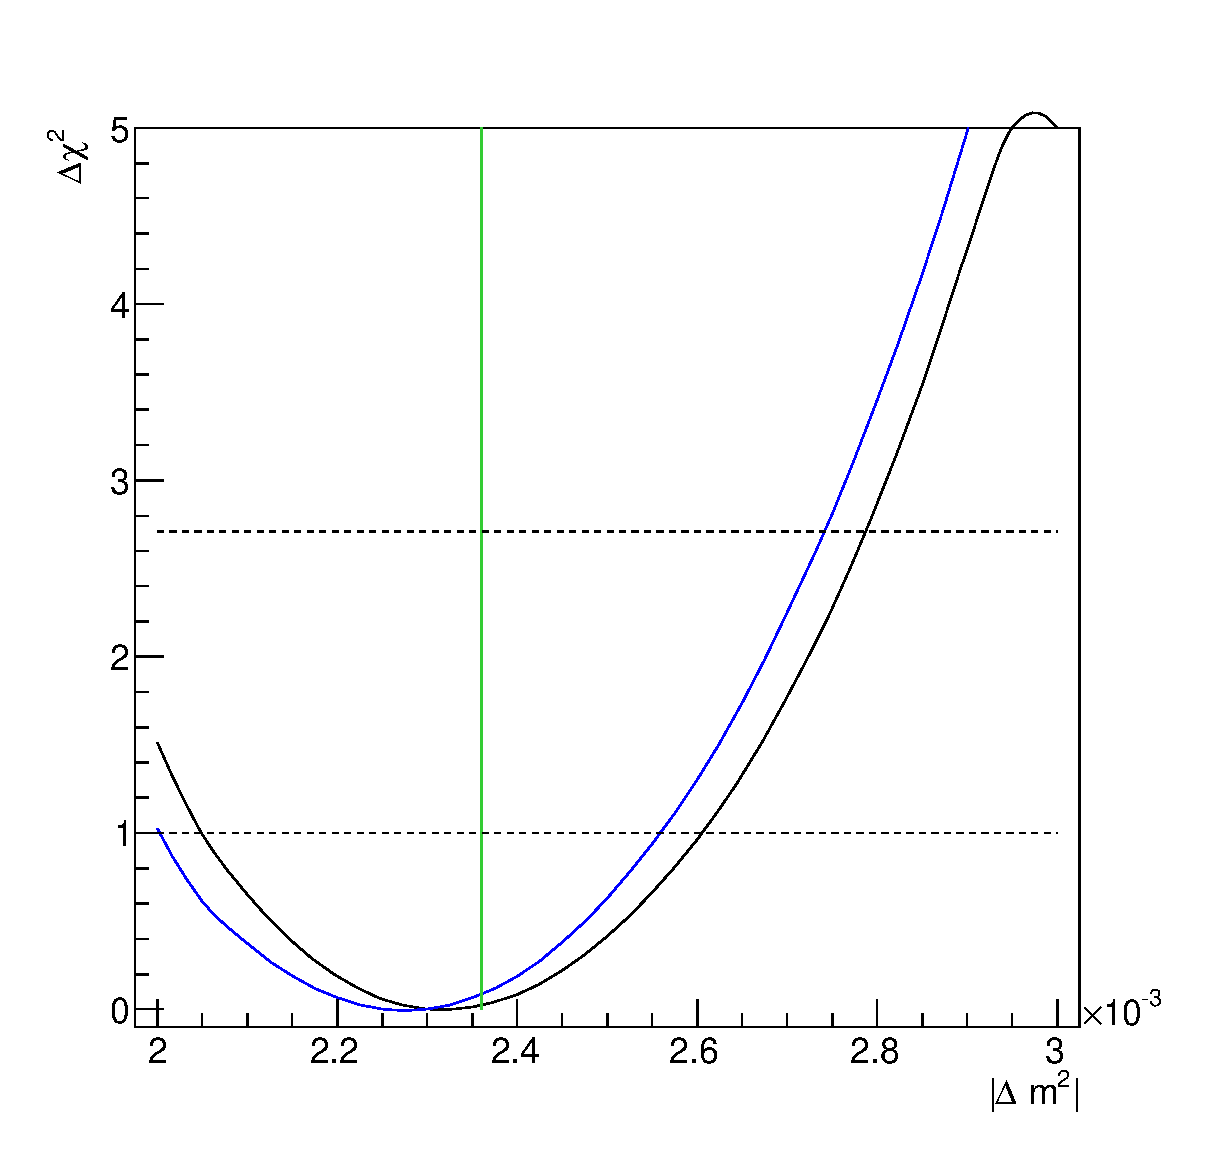
\includegraphics[width=9pc]{./images/appendix/fake_dataset_fits/realistic_fake_dataset2_chisq_dm23sq_global_min.eps}
\caption {
  $\Delta\chi^2$ as function of $|\Delta m^{2}|$ for fake dataset \#9.
  At each point, $\chi^2$ was minimized with respect to 
  $\sin^{2}\theta_{23}$, $\sin^{2}\theta_{13}$, $\delta_{CP}$
  and all relevant nuisance parameters for the joint analysis (black)
  and with respect to $\sin^{2}\theta_{23}$ and all relevant nuisance
  parameters for the disappearance analysis (blue).
}
\label{fig:toymc9_dchisq_Dmsq}
\end{minipage}
\hspace{0.02\linewidth}
\begin{minipage}[t]{0.22\linewidth}
\center
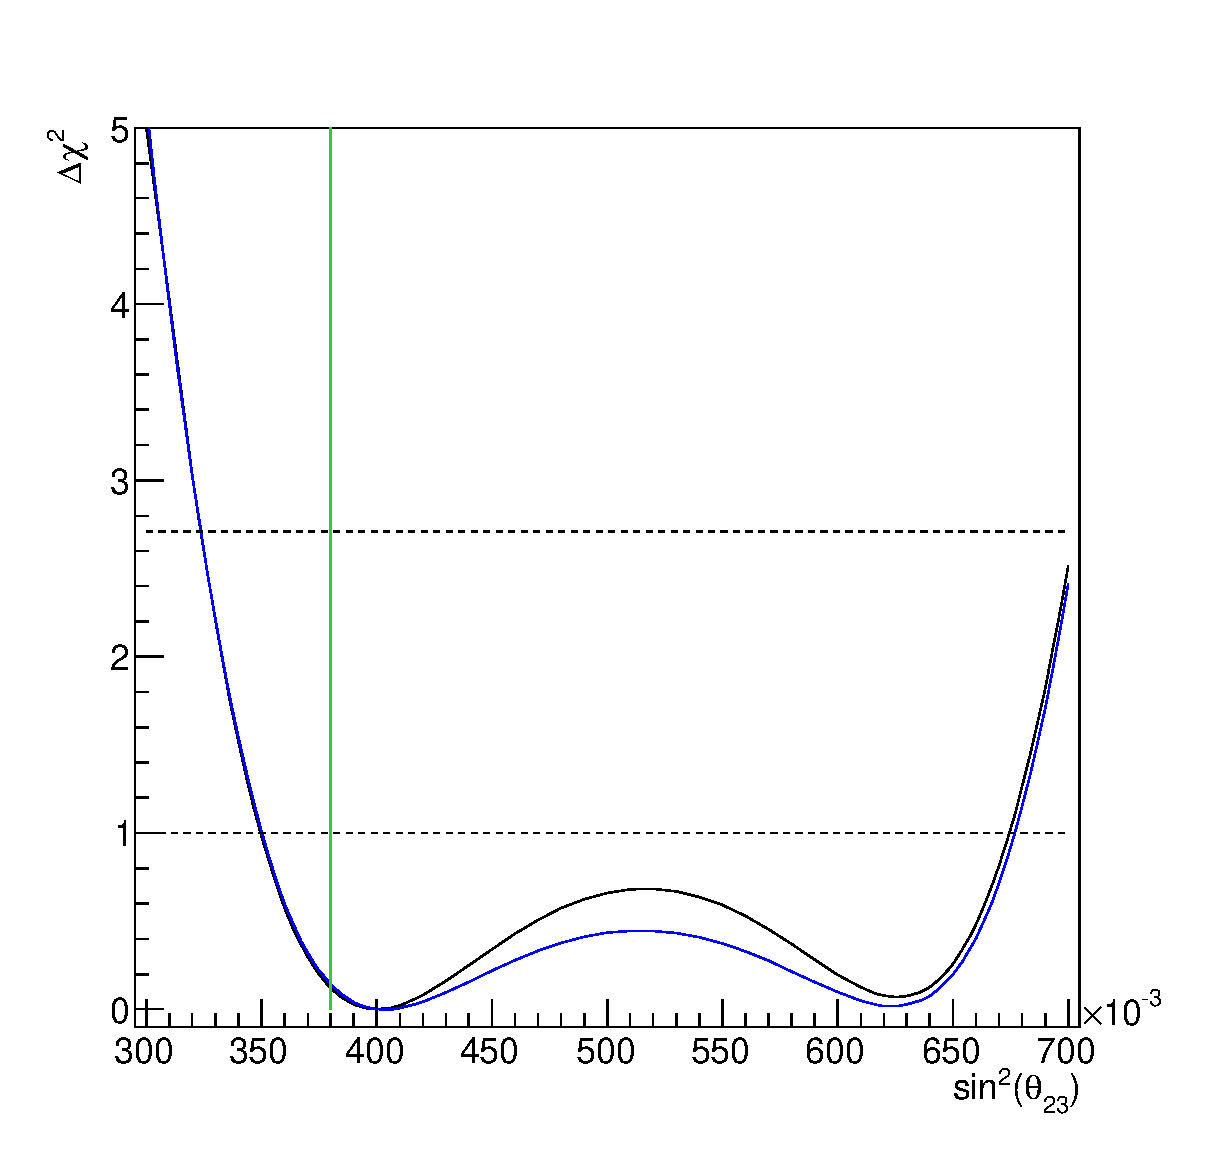
\includegraphics[width=9pc]{./images/appendix/fake_dataset_fits/realistic_fake_dataset2_chisq_theta23_global_min.eps}
\caption {
  $\Delta\chi^2$ as function of $sin^{2}\theta_{23}$ for fake dataset \#9.
  At each point, $\chi^2$ was minimized with respect to 
  $|\Delta m^{2}|$, $\sin^{2}\theta_{13}$, $\delta_{CP}$
  and all relevant nuisance parameters for the joint analysis (black)
  and with respect to $\sin^{2}\theta_{23}$ and all relevant nuisance
  parameters for the disappearance analysis (blue).
}
\label{fig:toymc9_dchisq_sinsqtheta23}
\end{minipage}
\hspace{0.02\linewidth}
\begin{minipage}[t]{0.22\linewidth}
\center
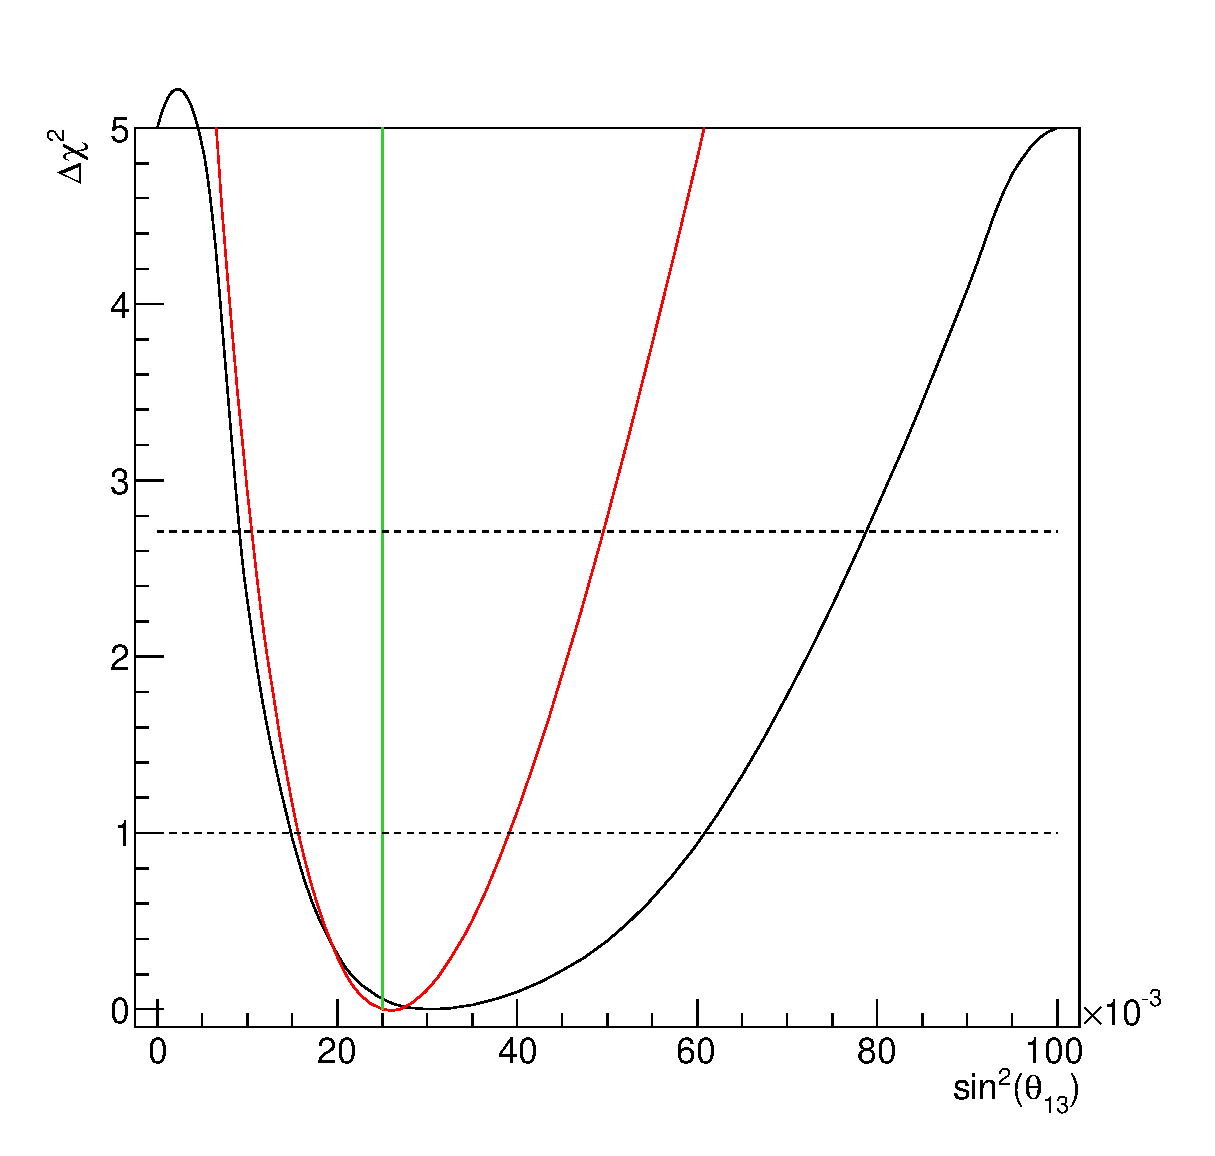
\includegraphics[width=9pc]{./images/appendix/fake_dataset_fits/realistic_fake_dataset2_chisq_theta13_global_min.eps}
\caption {
  $\Delta\chi^2$ as function of $sin^{2}\theta_{13}$ for fake dataset \#9.
  At each point, $\chi^2$ was minimized with respect to 
  $\sin^{2}\theta_{23}$, $\sin^{2}\theta_{13}$, $\delta_{CP}$
  and all relevant nuisance parameters for the joint analysis (black)
  and with respect to all relevant nuisance parameters 
  ($\delta_{CP}$ is fixed to 0) for the appearance analysis (red).
}
\label{fig:toymc9_dchisq_sinsqtheta13}
\end{minipage}
\hspace{0.02\linewidth}
\begin{minipage}[t]{0.22\linewidth}
\center
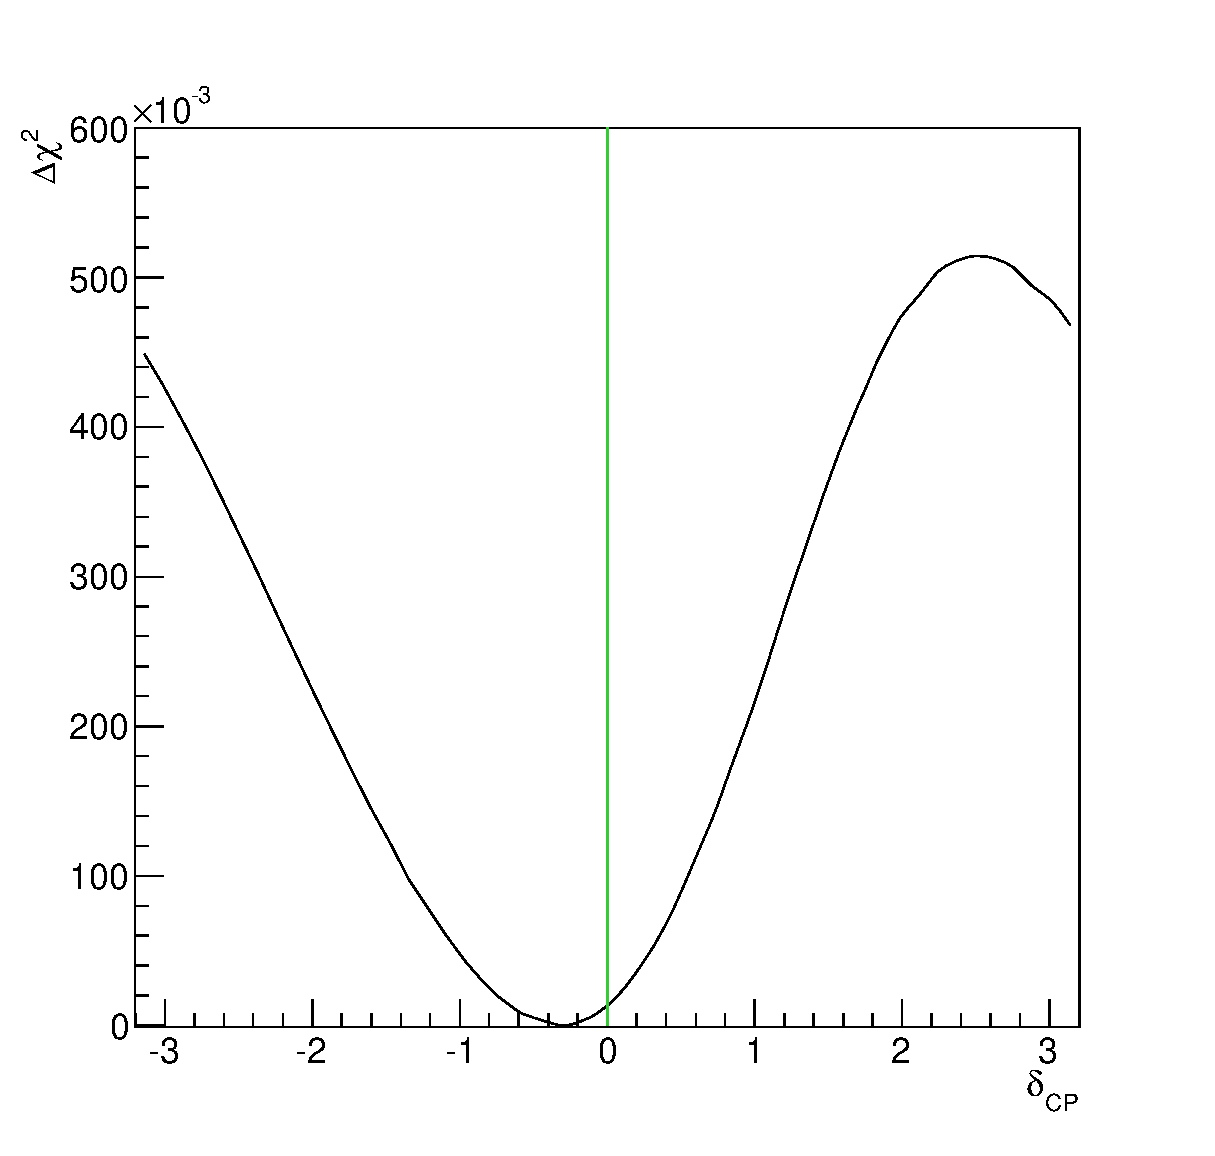
\includegraphics[width=9pc]{.//images/appendix/fake_dataset_fits/realistic_fake_dataset2_chisq_deltacp_global_min.eps}
\caption {
  $\Delta\chi^2$ as function of $\delta_{CP}$ for fake dataset \#9.
  At each point, $\chi^2$ was minimized with respect to 
  all oscillation parameters not shown (and not considered to be fixed)
  and all relevant nuisance parameters.
}
\label{fig:toymc9_dchisq_deltacp}
\end{minipage}
\vfill
\vspace*{0.7cm}
\begin{minipage}[t]{0.48\linewidth}
\center
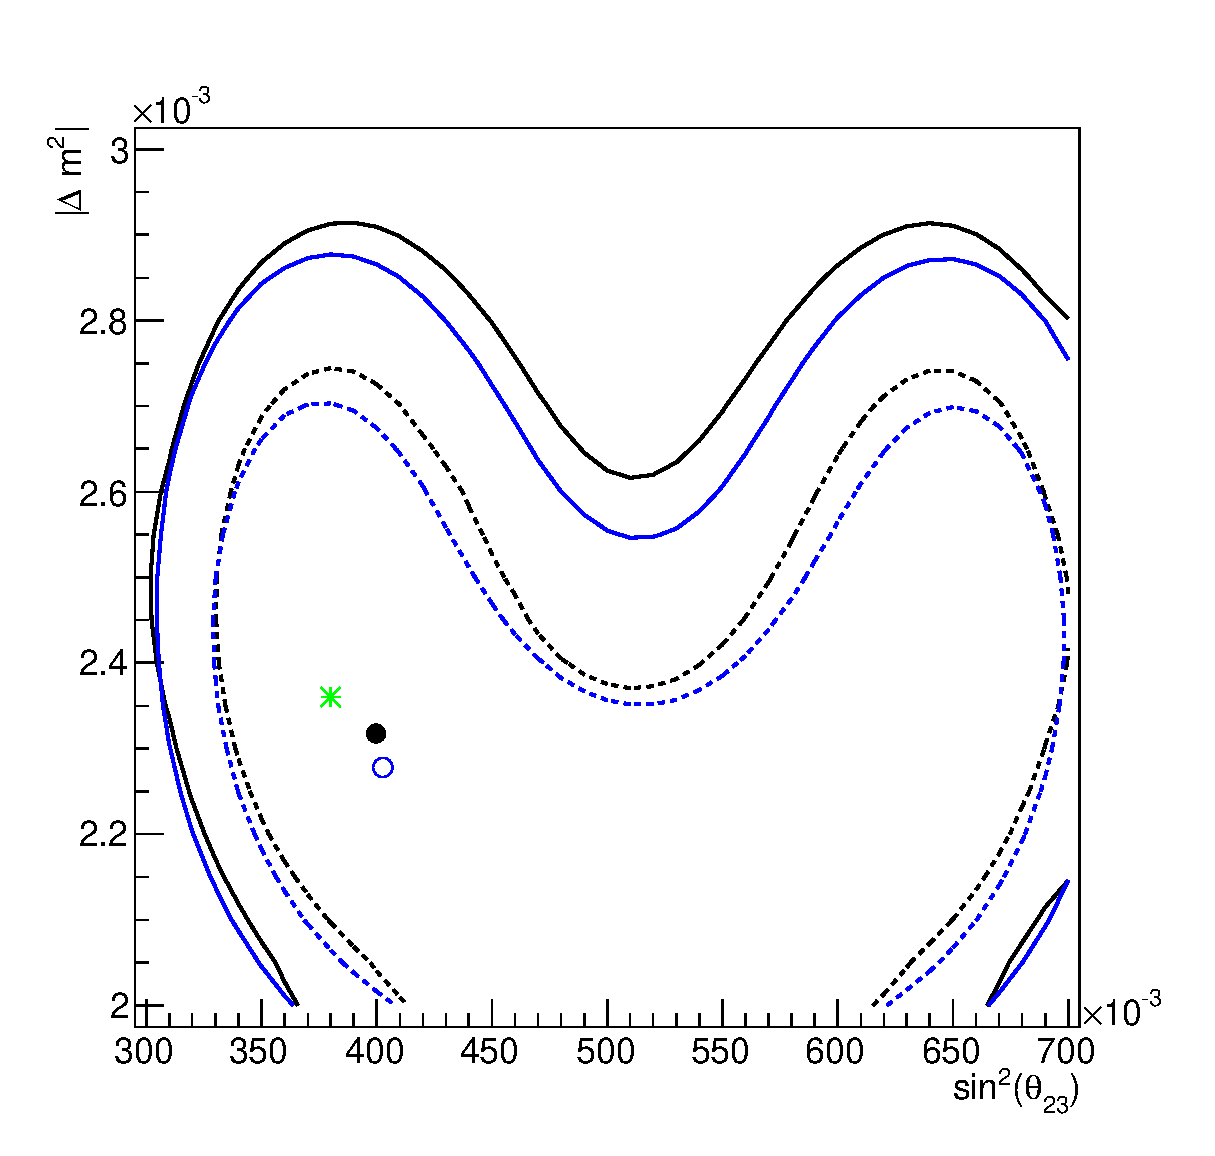
\includegraphics[width=15pc]{./images/appendix/fake_dataset_fits/realistic_fake_dataset2_chisq_theta23_dm23sq_global_min.eps}
\caption {
  68\% and 90\% CL regions in ($sin^{2}\theta_{23}$, $|\Delta m^{2}|$) space for fake dataset \#9.
  At each point, $\chi^2$ was minimized with respect to 
  $\sin^{2}\theta_{13}$, $\delta_{CP}$
  and all relevant nuisance parameters for the joint analysis (black)
  and with respect to all relevant nuisance parameters for the disappearance analysis (blue).
}
\label{fig:toymc9_confreg_sinsqtheta23_Dmsq}
\end{minipage}
\hspace{0.03\linewidth}
\begin{minipage}[t]{0.48\linewidth}
\center
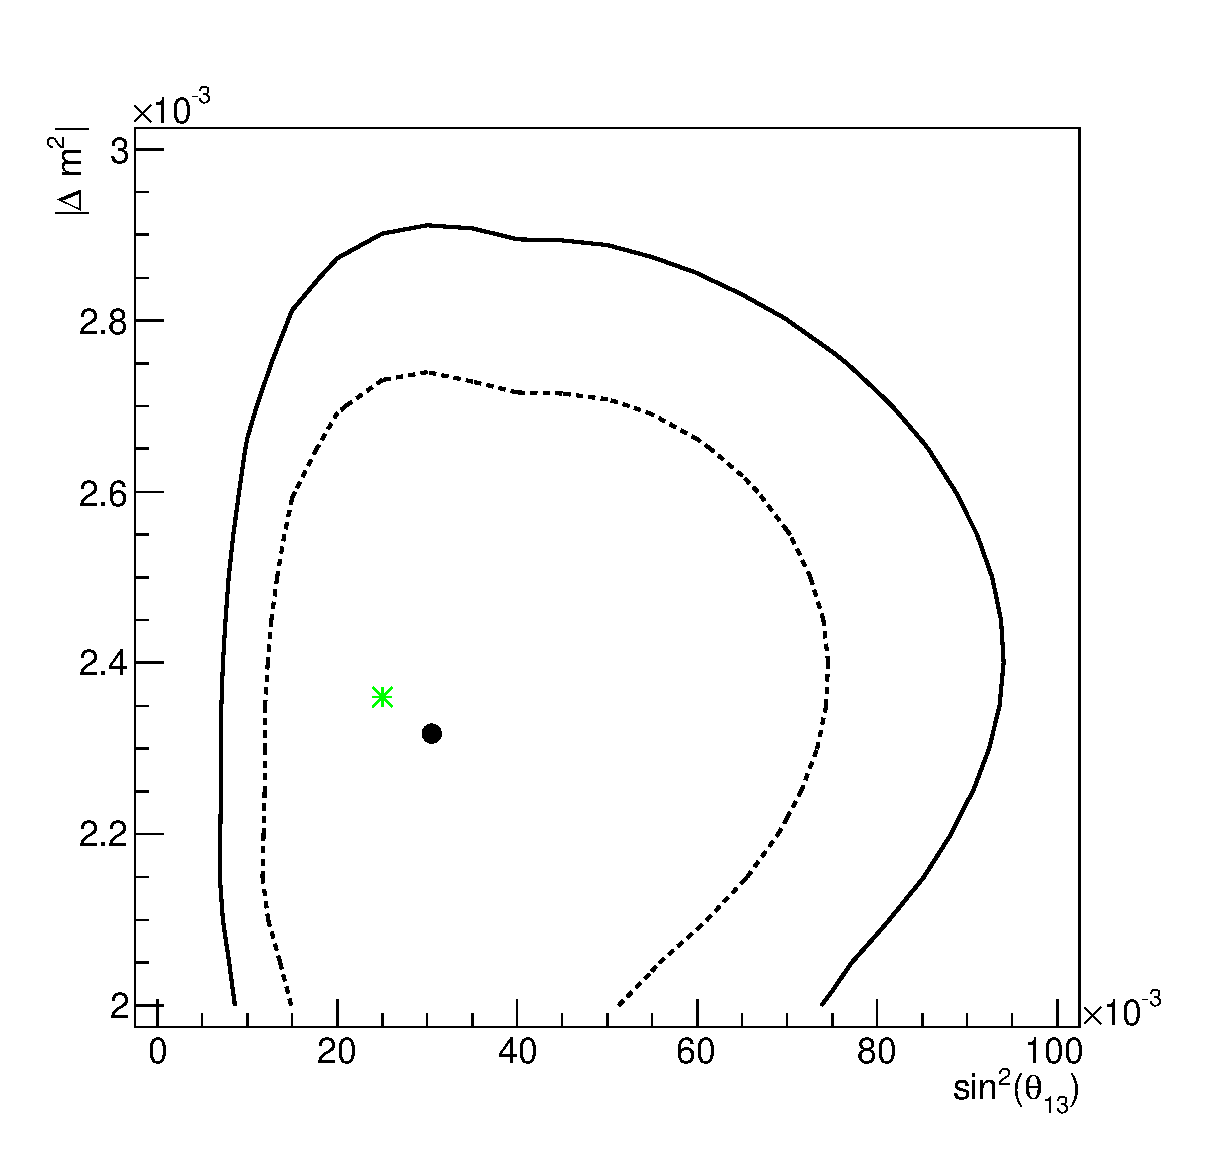
\includegraphics[width=15pc]{./images/appendix/fake_dataset_fits/realistic_fake_dataset2_chisq_theta13_dm23sq_global_min.eps}
\caption {
  68\% and 90\% CL regions in ($sin^{2}\theta_{13}$, $|\Delta m^{2}|$) space for fake dataset \#9.
  At each point, $\chi^2$ was minimized with respect to 
  all oscillation parameters not shown (and not considered to be fixed)
  and all relevant nuisance parameters.
}
\label{fig:toymc9_confreg_sinsqtheta13_Dmsq}
\end{minipage}

\vfill
\vspace*{0.7cm}

\begin{minipage}[t]{0.48\linewidth}
\center
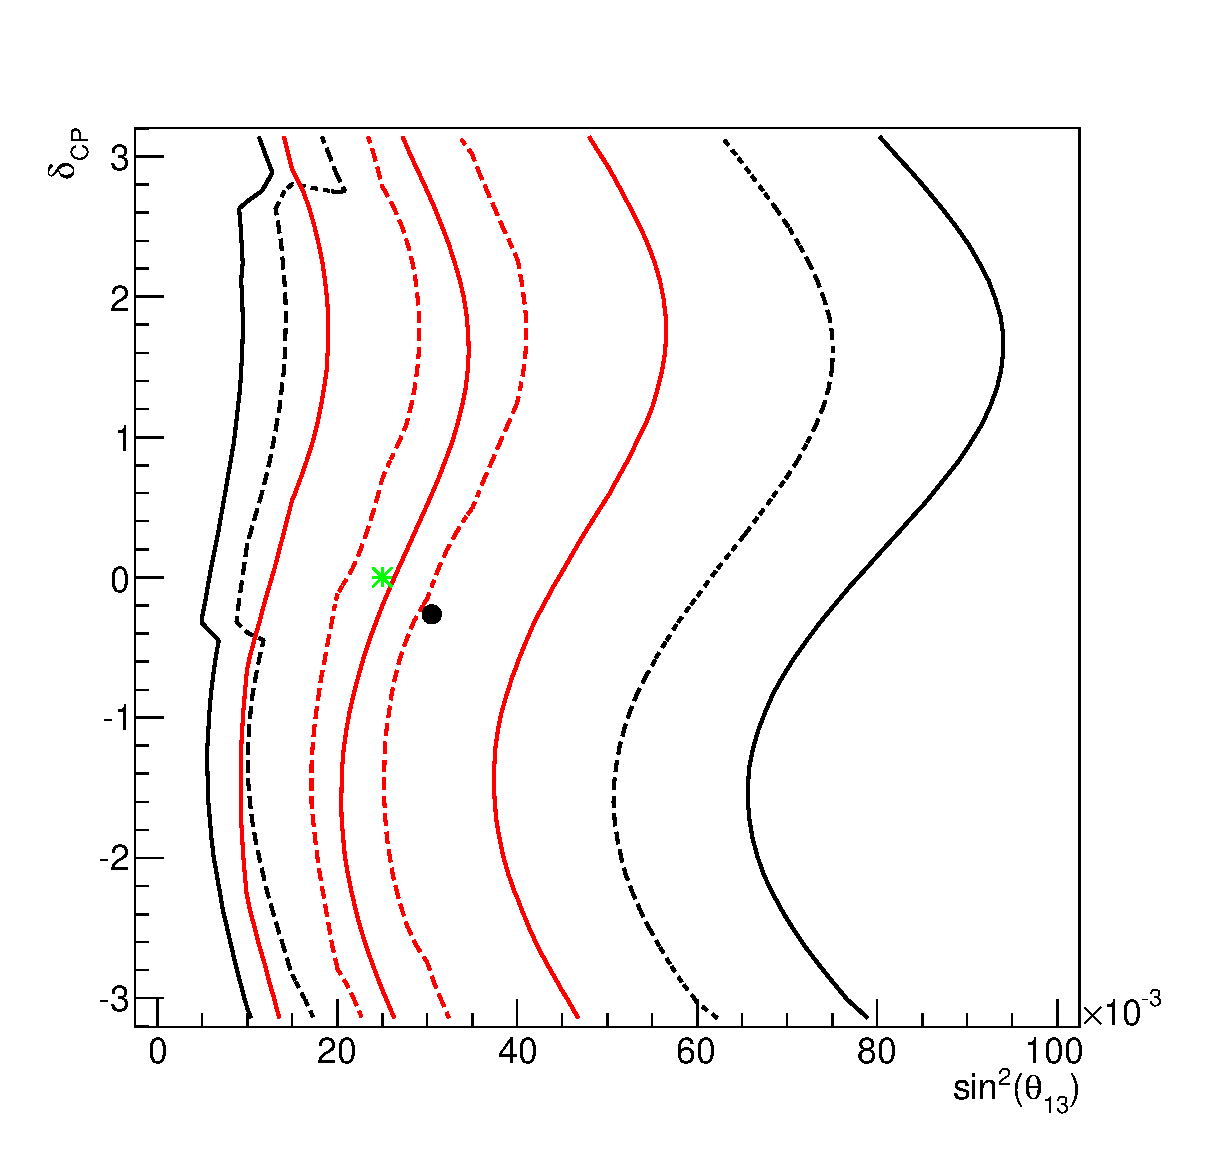
\includegraphics[width=15pc]{./images/appendix/fake_dataset_fits/realistic_fake_dataset2_chisq_theta13_deltacp_global_min.eps}
\caption {
  68\% and 90\% CL regions in ($sin^{2}\theta_{13}$, $\delta_{CP}$) space for fake dataset \#9.
  At each point, $\chi^2$ was minimized with respect to 
  $|\Delta m^{2}|$, $\sin^{2}\theta_{23}$
  and all relevant nuisance parameters for the joint analysis (black)
  and with respect to all relevant nuisance parameters for the appearance analysis (red).
  Notice that different methods are used to
  construct confidence regions for the joint analysis (global minimum) and for the 
  stand-alone appearance analysis (raster scan).
}
\label{fig:toymc9_confreg_sinsqtheta13_deltacp}
\end{minipage}
\hspace{0.03\linewidth}
\begin{minipage}[t]{0.48\linewidth}
\center
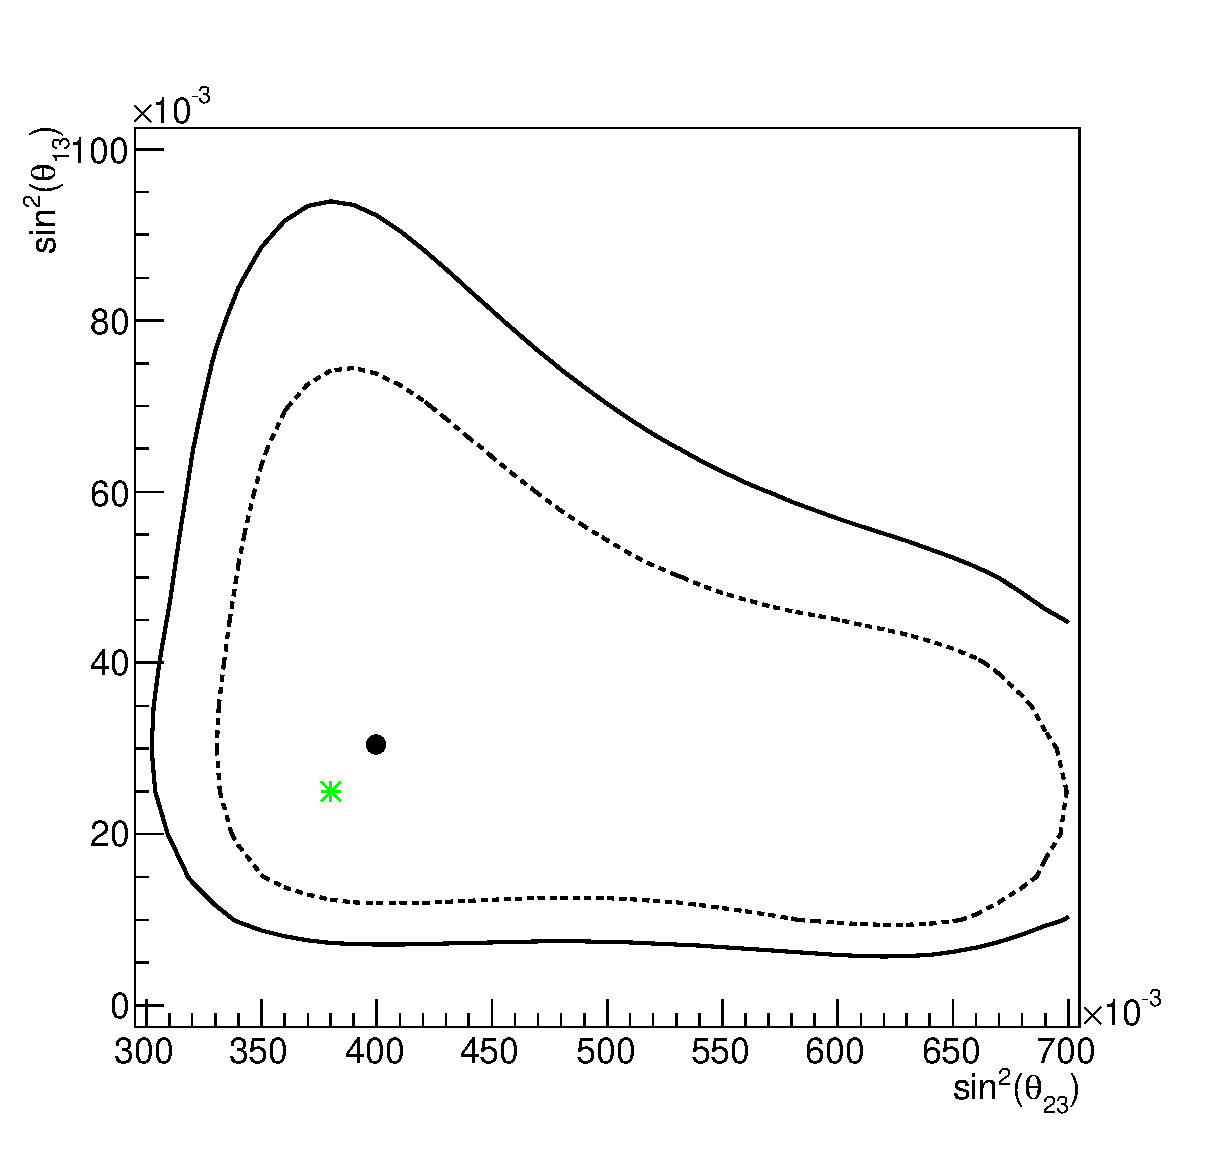
\includegraphics[width=15pc]{./images/appendix/fake_dataset_fits/realistic_fake_dataset2_chisq_theta13_theta23_global_min.eps}
\caption {
  68\% and 90\% CL regions in ($sin^{2}\theta_{23}$, $sin^{2}\theta_{13}$) space for fake dataset \#9.
  At each point, $\chi^2$ was minimized with respect to 
  all oscillation parameters not shown (and not considered to be fixed)
  and all relevant nuisance parameters.
}
\label{fig:toymc9_confreg_sinsqtheta23_sinsqtheta13}
\end{minipage}

\end{figure*}





% 
% 
% ..............................................
% Fake dataset #10
% 
%

\clearpage
\begin{figure*}[htb]

\begin{minipage}[t]{0.46\linewidth}
\center
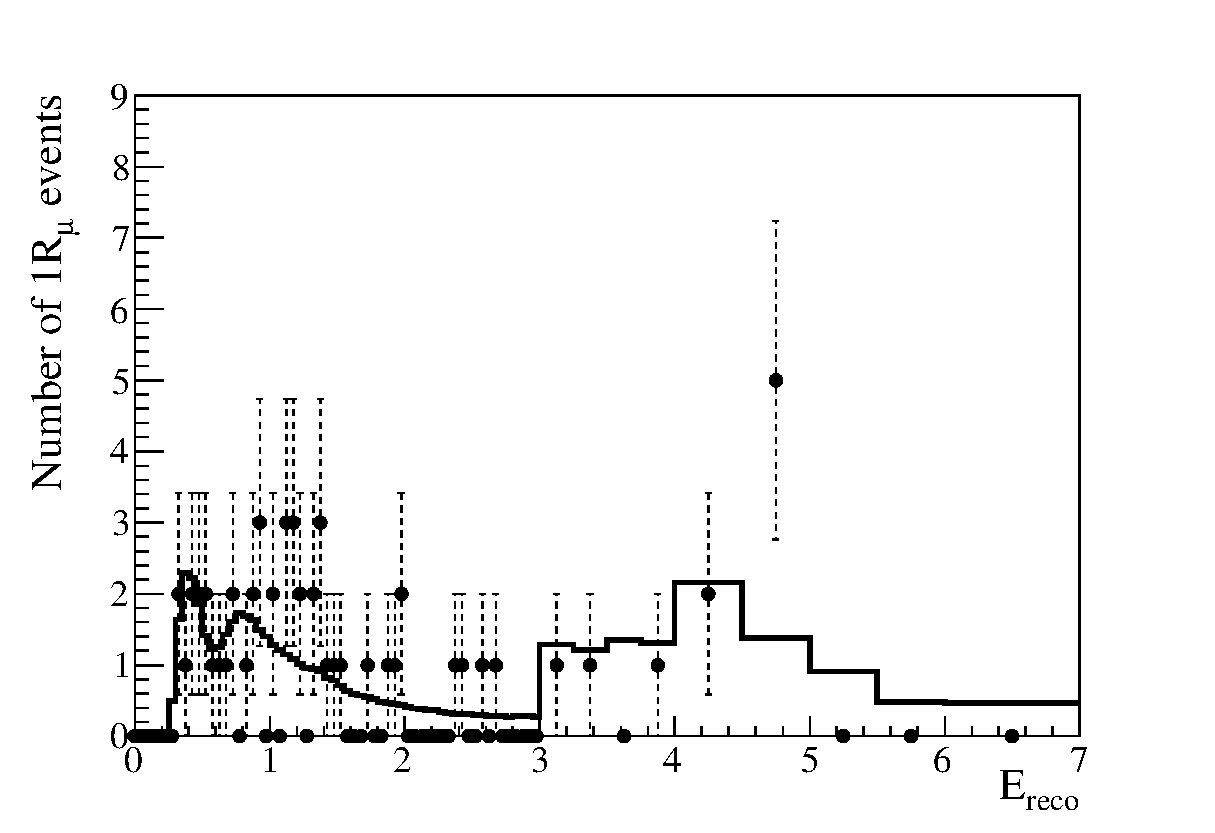
\includegraphics[width=15pc]{./images/appendix/fake_dataset_fits/realistic_fake_dataset3_nh_1st_1Rmu.eps}
\caption {
  Single $\mu$-like ring event best-fit reconstructed energy spectrum
  to fake dataset \#10.
}
\label{fig:toymc10_1Rmu_bestfit_spectrum}
\end{minipage}
\hspace{0.03\linewidth}
\begin{minipage}[t]{0.46\linewidth}
\center
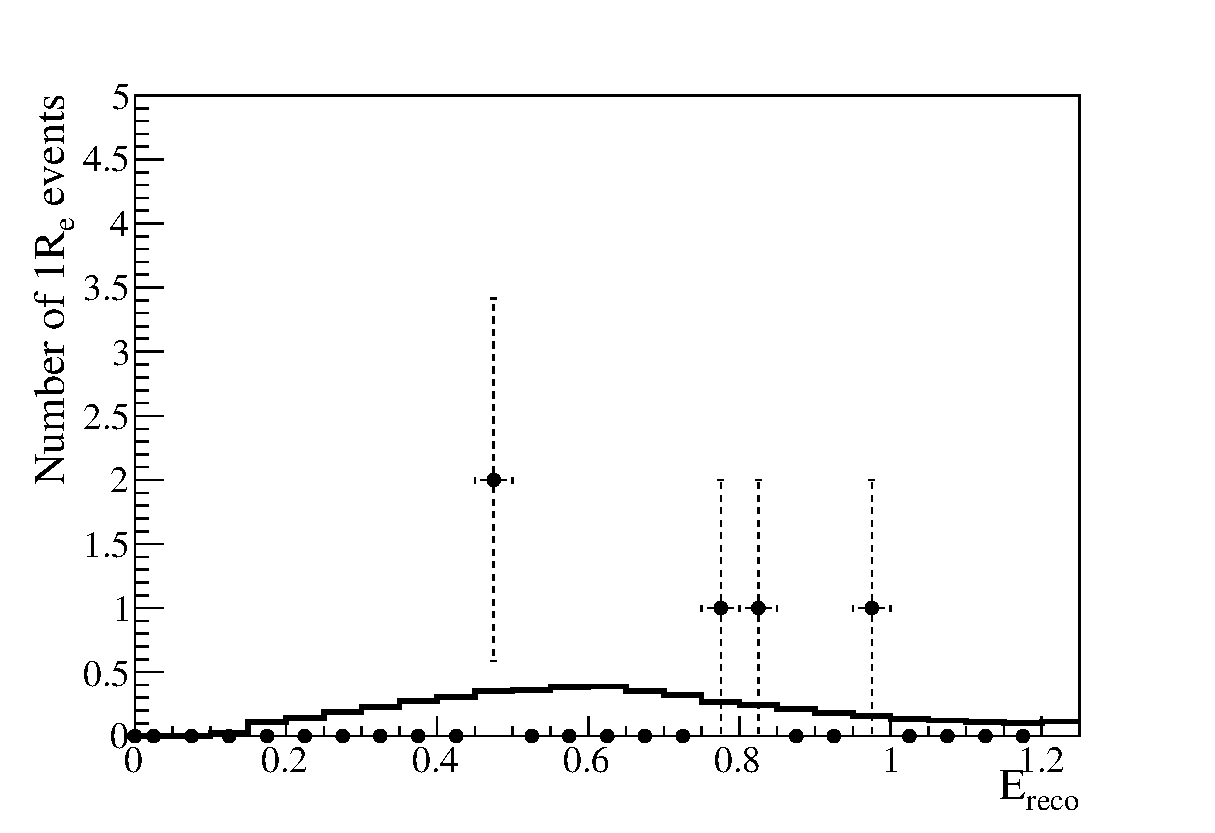
\includegraphics[width=15pc]{./images/appendix/fake_dataset_fits/realistic_fake_dataset3_nh_1st_1Re.eps}
\caption {
  Single e-like ring event best-fit reconstructed energy spectrum
  to fake dataset \#10.
}
\label{fig:toymc10_1Re_bestfit_spectrum}
\end{minipage}

\vfill
\vspace*{0.7cm}

\begin{minipage}[t]{0.90\linewidth}
\center
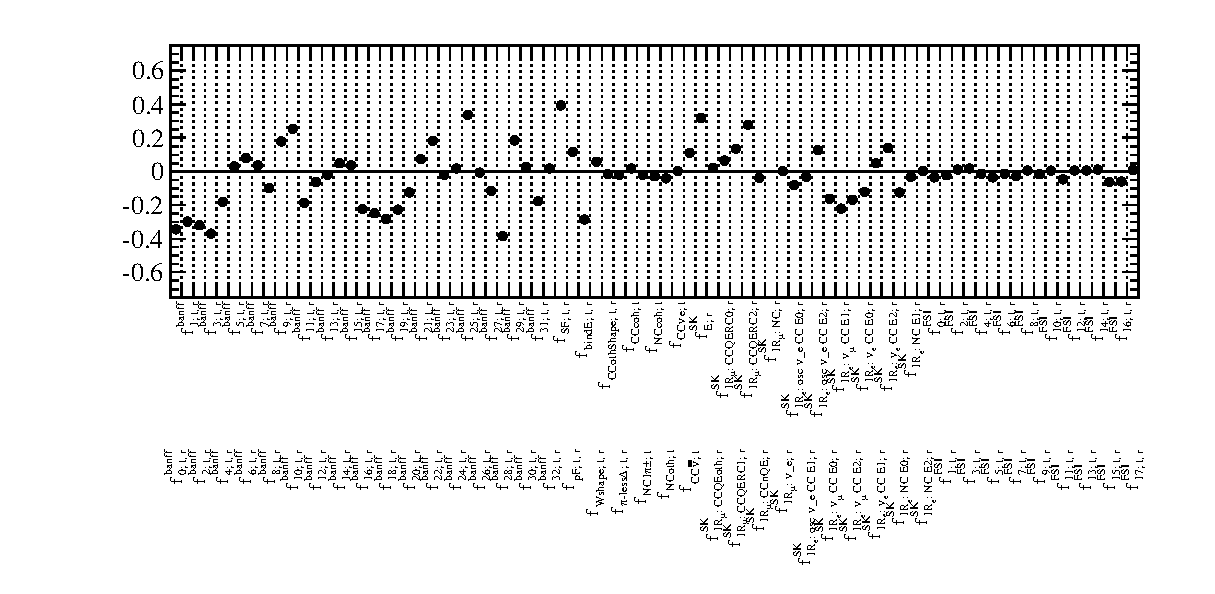
\includegraphics[width=30pc,angle=270]{./images/appendix/fake_dataset_fits/pulls_realistic_fake_dataset3_nh_1st.eps}
\caption {
  Systematic parameter pulls for the oscillation fit to fake dataset \#10.
}
\label{fig:toymc10_pulls}
\end{minipage}

\end{figure*}


%...........................................................
%
% chisq distributions used for calculating the fit p-values
%

\begin{figure*}[htb]

\begin{minipage}[t]{0.90\linewidth}
\center
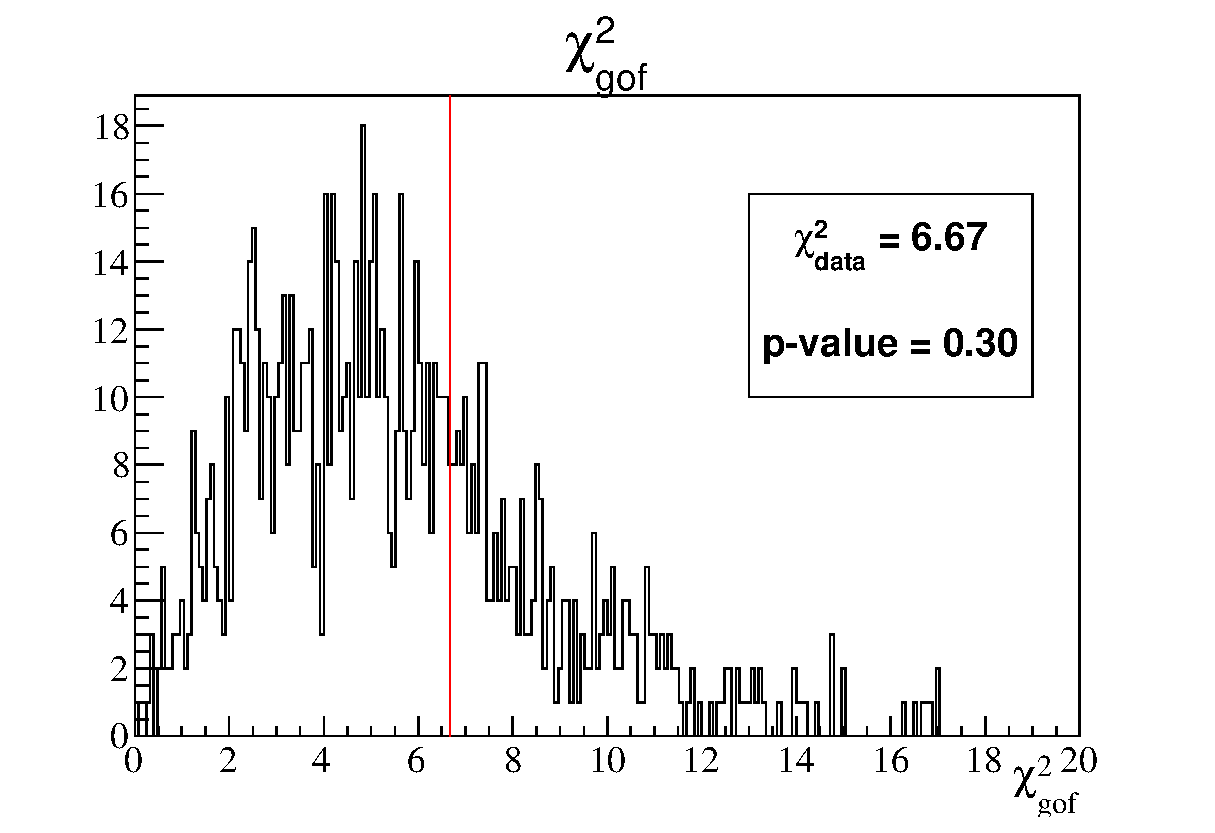
\includegraphics[width=30pc]{./images/appendix/fake_dataset_fits/realistic_fake_dataset3_nh_1st_gof_new.eps}
\caption {
  Distribution of $\chi^2_{gof}$, the goodness-of-fit (gof) $\chi^2$, 
  from 1k toy MC experiments generated at dataset \#10 joint 3-flavour analysis best-fit oscillation point.
  The $\chi^2_{gof}$ value for the dataset \#10 ($\chi^2_{data}$) is highlighted.
  All $\chi^2_{gof}$ values were computed 
  using the 5 (single $\mu$-like ring) + 3 (single e-like ring) 
  reconstructed energy binning scheme described in Sec.\ \ref{sec:goodness_of_fit}.
}
\label{fig:toymc10_gofchisq}
\end{minipage}

\vfill
\vspace*{0.7cm}

\begin{minipage}[t]{0.46\linewidth}
\center
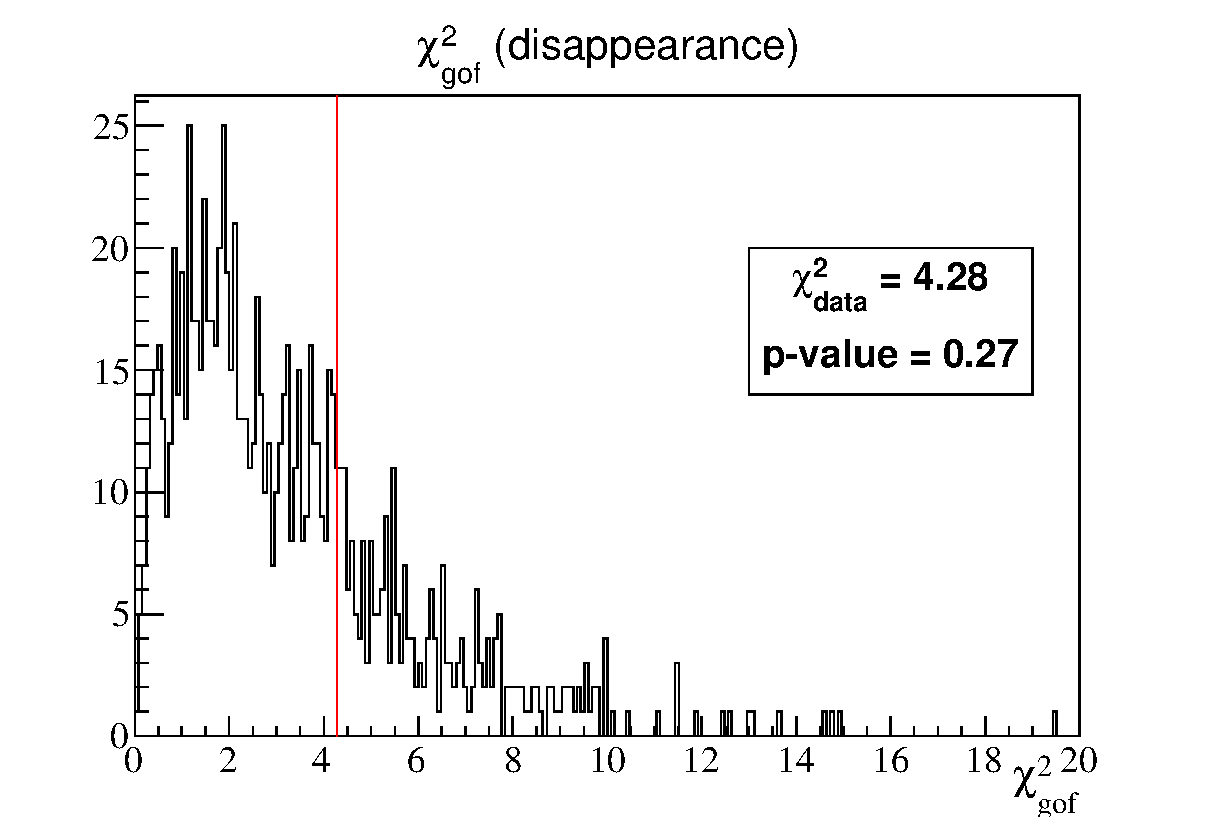
\includegraphics[width=18pc]{./images/appendix/fake_dataset_fits/realistic_fake_dataset3_nh_1st_gof_disap_new.eps}
\caption {
  Distribution of $\chi^2_{gof}$
  from 1k toy MC experiments generated at the dataset \#10 stand-alone 3-flavour $\nu_{\mu}$ disappearance analysis best-fit oscillation point.
  The $\chi^2_{gof}$ value for the dataset \#10 ($\chi^2_{data}$) is highlighted.
  All $\chi^2_{gof}$ values were computed 
  using the 5 (single $\mu$-like ring) 
  reconstructed energy binning scheme described in Sec.\ \ref{sec:goodness_of_fit}.
}
\label{fig:toymc10_gofchisq_disapp}
\end{minipage}
\hspace{0.03\linewidth}
\begin{minipage}[t]{0.46\linewidth}
\center
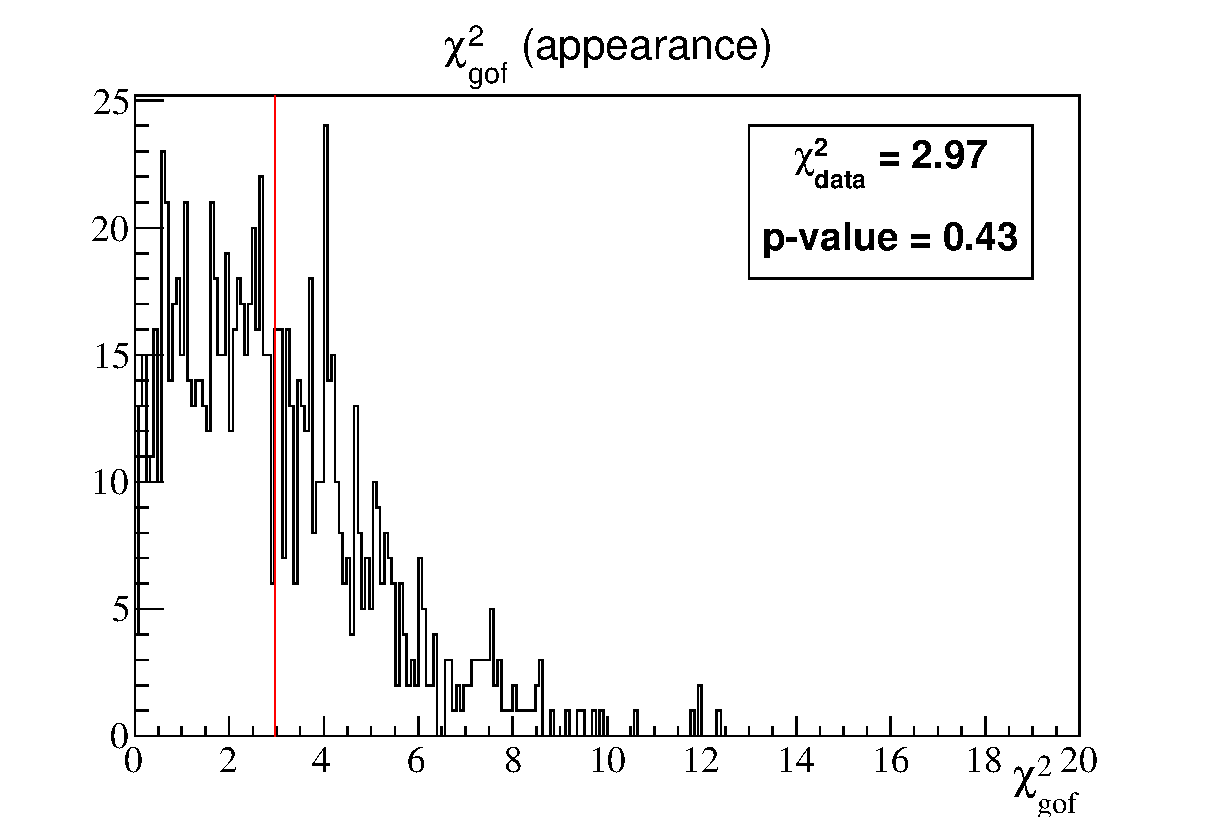
\includegraphics[width=18pc]{./images/appendix/fake_dataset_fits/realistic_fake_dataset3_nh_1st_gof_app_new.eps}
\caption {
  Distribution of $\chi^2_{gof}$
  from 1k toy MC experiments generated at the dataset \#10 stand-alone 3-flavour $\nu_{e}$ appearance analysis best-fit oscillation point.
  The $\chi^2_{gof}$ value for the dataset \#10 ($\chi^2_{data}$) is highlighted.
  All $\chi^2_{gof}$ values were computed 
  using the 3 (single e-like ring) 
  reconstructed energy binning scheme  as described in Sec.\ \ref{sec:goodness_of_fit}.
}
\label{fig:toymc10_gofchisq_app}
\end{minipage}

\end{figure*}



%
% delta\chisq and contours
%

\begin{figure*}[htb]

\begin{minipage}[t]{0.22\linewidth}
\center
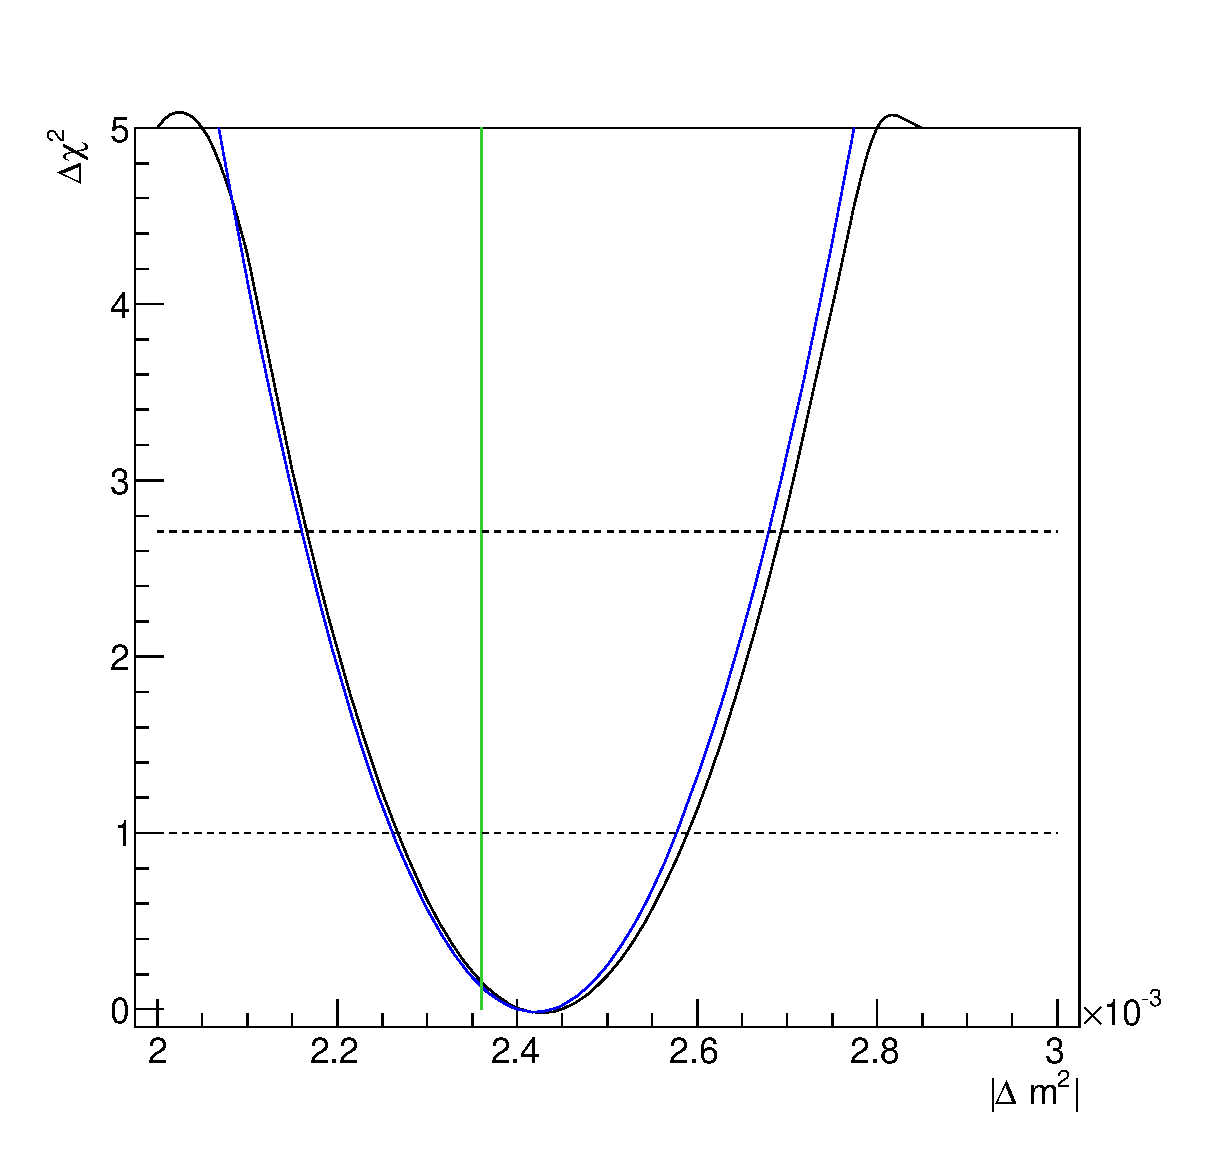
\includegraphics[width=9pc]{./images/appendix/fake_dataset_fits/realistic_fake_dataset3_chisq_dm23sq_global_min.eps}
\caption {
  $\Delta\chi^2$ as function of $|\Delta m^{2}|$ for fake dataset \#10.
  At each point, $\chi^2$ was minimized with respect to 
  $\sin^{2}\theta_{23}$, $\sin^{2}\theta_{13}$, $\delta_{CP}$
  and all relevant nuisance parameters for the joint analysis (black)
  and with respect to $\sin^{2}\theta_{23}$ and all relevant nuisance
  parameters for the disappearance analysis (blue).
}
\label{fig:toymc10_dchisq_Dmsq}
\end{minipage}
\hspace{0.02\linewidth}
\begin{minipage}[t]{0.22\linewidth}
\center
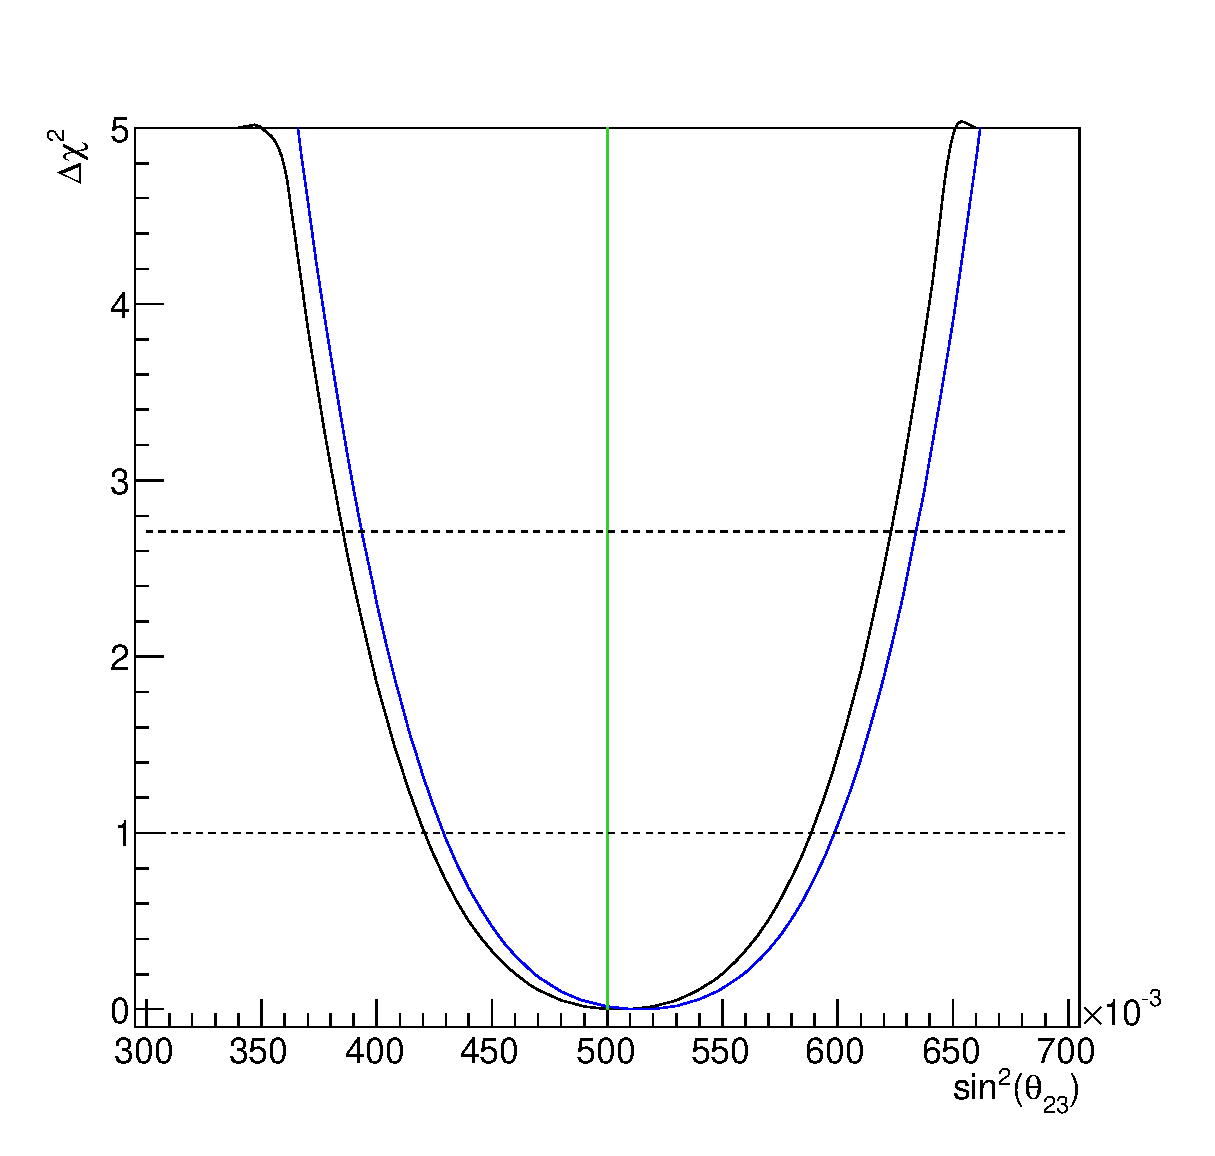
\includegraphics[width=9pc]{./images/appendix/fake_dataset_fits/realistic_fake_dataset3_chisq_theta23_global_min.eps}
\caption {
  $\Delta\chi^2$ as function of $sin^{2}\theta_{23}$ for fake dataset \#10.
  At each point, $\chi^2$ was minimized with respect to 
  $|\Delta m^{2}|$, $\sin^{2}\theta_{13}$, $\delta_{CP}$
  and all relevant nuisance parameters for the joint analysis (black)
  and with respect to $\sin^{2}\theta_{23}$ and all relevant nuisance
  parameters for the disappearance analysis (blue).
}
\label{fig:toymc10_dchisq_sinsqtheta23}
\end{minipage}
\hspace{0.02\linewidth}
\begin{minipage}[t]{0.22\linewidth}
\center
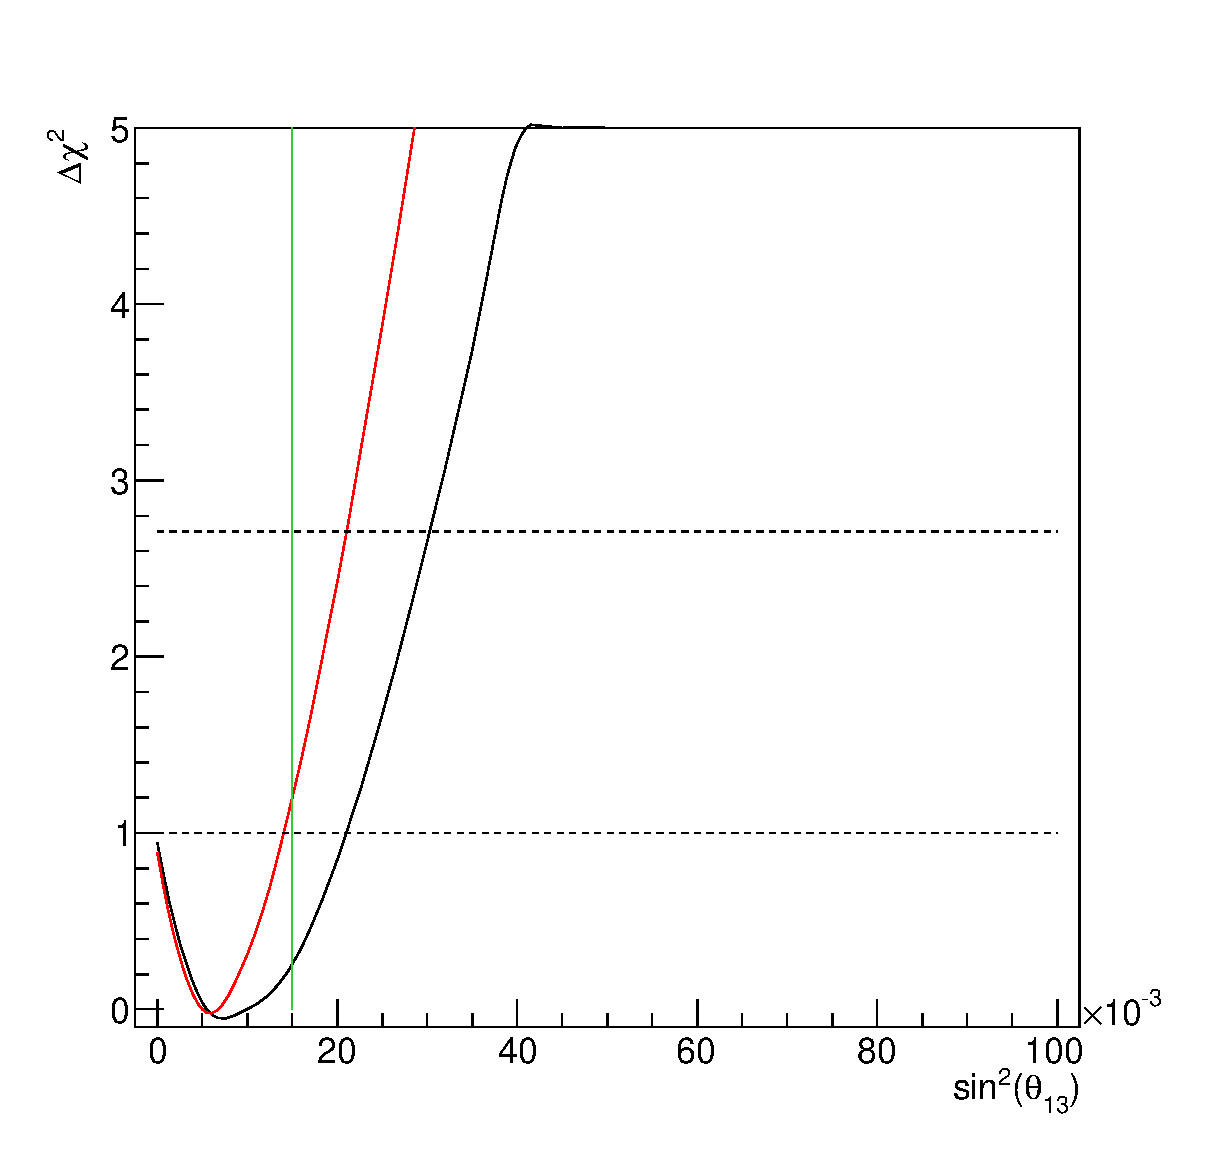
\includegraphics[width=9pc]{./images/appendix/fake_dataset_fits/realistic_fake_dataset3_chisq_theta13_global_min.eps}
\caption {
  $\Delta\chi^2$ as function of $sin^{2}\theta_{13}$ for fake dataset \#10.
  At each point, $\chi^2$ was minimized with respect to 
  $\sin^{2}\theta_{23}$, $\sin^{2}\theta_{13}$, $\delta_{CP}$
  and all relevant nuisance parameters for the joint analysis (black)
  and with respect to all relevant nuisance parameters 
  ($\delta_{CP}$ is fixed to 0) for the appearance analysis (red).
}
\label{fig:toymc10_dchisq_sinsqtheta13}
\end{minipage}
\hspace{0.02\linewidth}
\begin{minipage}[t]{0.22\linewidth}
\center
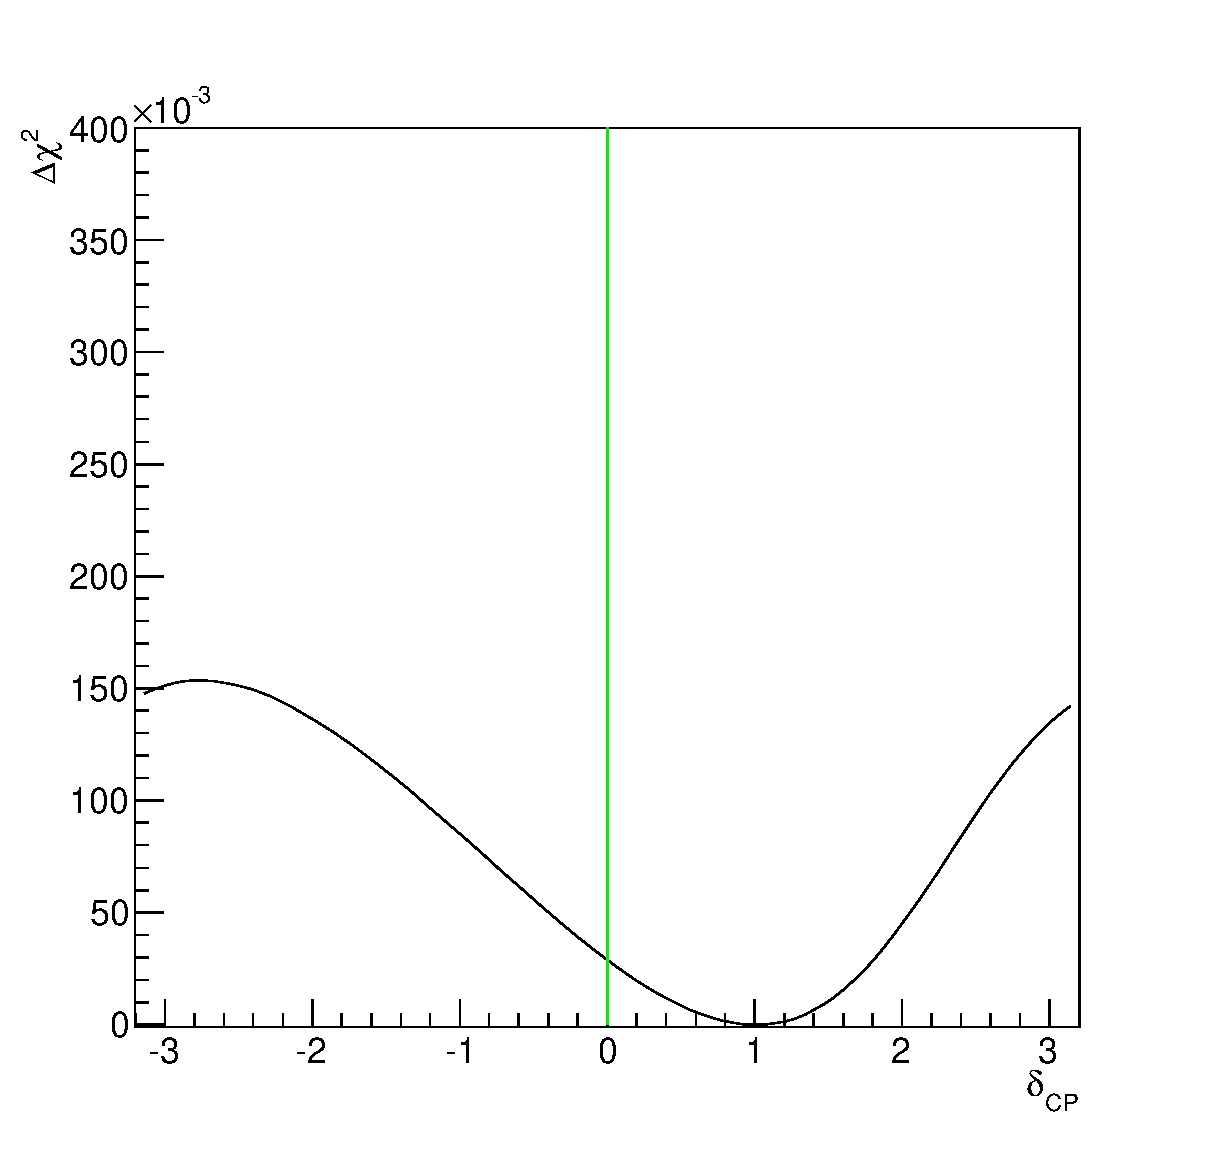
\includegraphics[width=9pc]{.//images/appendix/fake_dataset_fits/realistic_fake_dataset3_chisq_deltacp_global_min.eps}
\caption {
  $\Delta\chi^2$ as function of $\delta_{CP}$ for fake dataset \#10.
  At each point, $\chi^2$ was minimized with respect to 
  all oscillation parameters not shown (and not considered to be fixed)
  and all relevant nuisance parameters.
}
\label{fig:toymc10_dchisq_deltacp}
\end{minipage}
\vfill
\vspace*{0.7cm}
\begin{minipage}[t]{0.48\linewidth}
\center
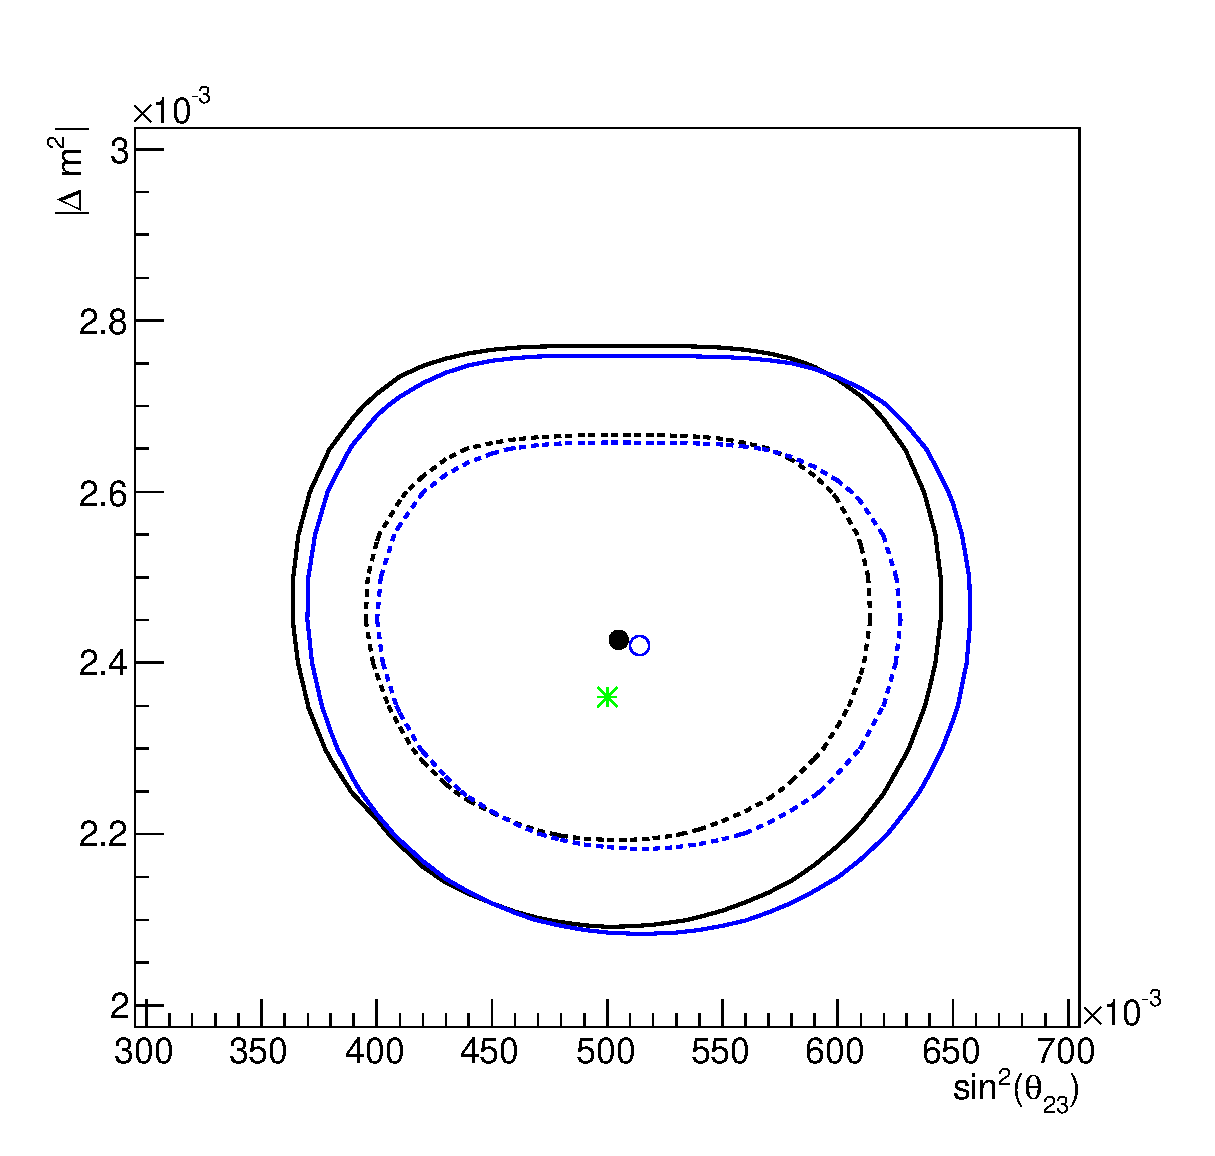
\includegraphics[width=15pc]{./images/appendix/fake_dataset_fits/realistic_fake_dataset3_chisq_theta23_dm23sq_global_min.eps}
\caption {
  68\% and 90\% CL regions in ($sin^{2}\theta_{23}$, $|\Delta m^{2}|$) space for fake dataset \#10.
  At each point, $\chi^2$ was minimized with respect to 
  $\sin^{2}\theta_{13}$, $\delta_{CP}$
  and all relevant nuisance parameters for the joint analysis (black)
  and with respect to all relevant nuisance parameters for the disappearance analysis (blue).
}
\label{fig:toymc10_confreg_sinsqtheta23_Dmsq}
\end{minipage}
\hspace{0.03\linewidth}
\begin{minipage}[t]{0.48\linewidth}
\center
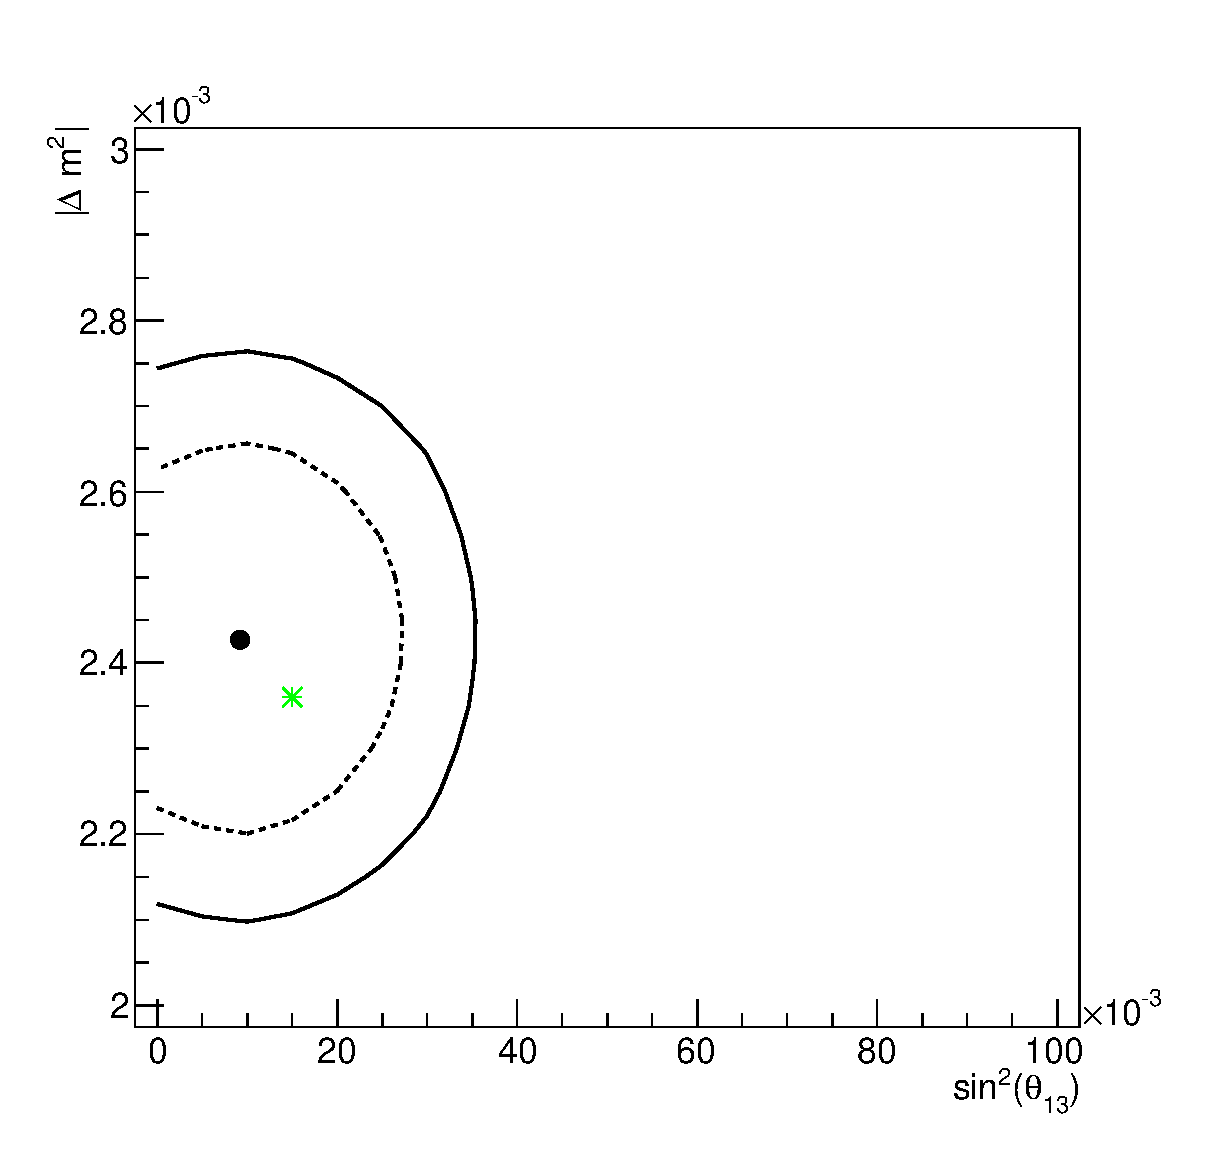
\includegraphics[width=15pc]{./images/appendix/fake_dataset_fits/realistic_fake_dataset3_chisq_theta13_dm23sq_global_min.eps}
\caption {
  68\% and 90\% CL regions in ($sin^{2}\theta_{13}$, $|\Delta m^{2}|$) space for fake dataset \#10.
  At each point, $\chi^2$ was minimized with respect to 
  all oscillation parameters not shown (and not considered to be fixed)
  and all relevant nuisance parameters.
}
\label{fig:toymc10_confreg_sinsqtheta13_Dmsq}
\end{minipage}

\vfill
\vspace*{0.7cm}

\begin{minipage}[t]{0.48\linewidth}
\center
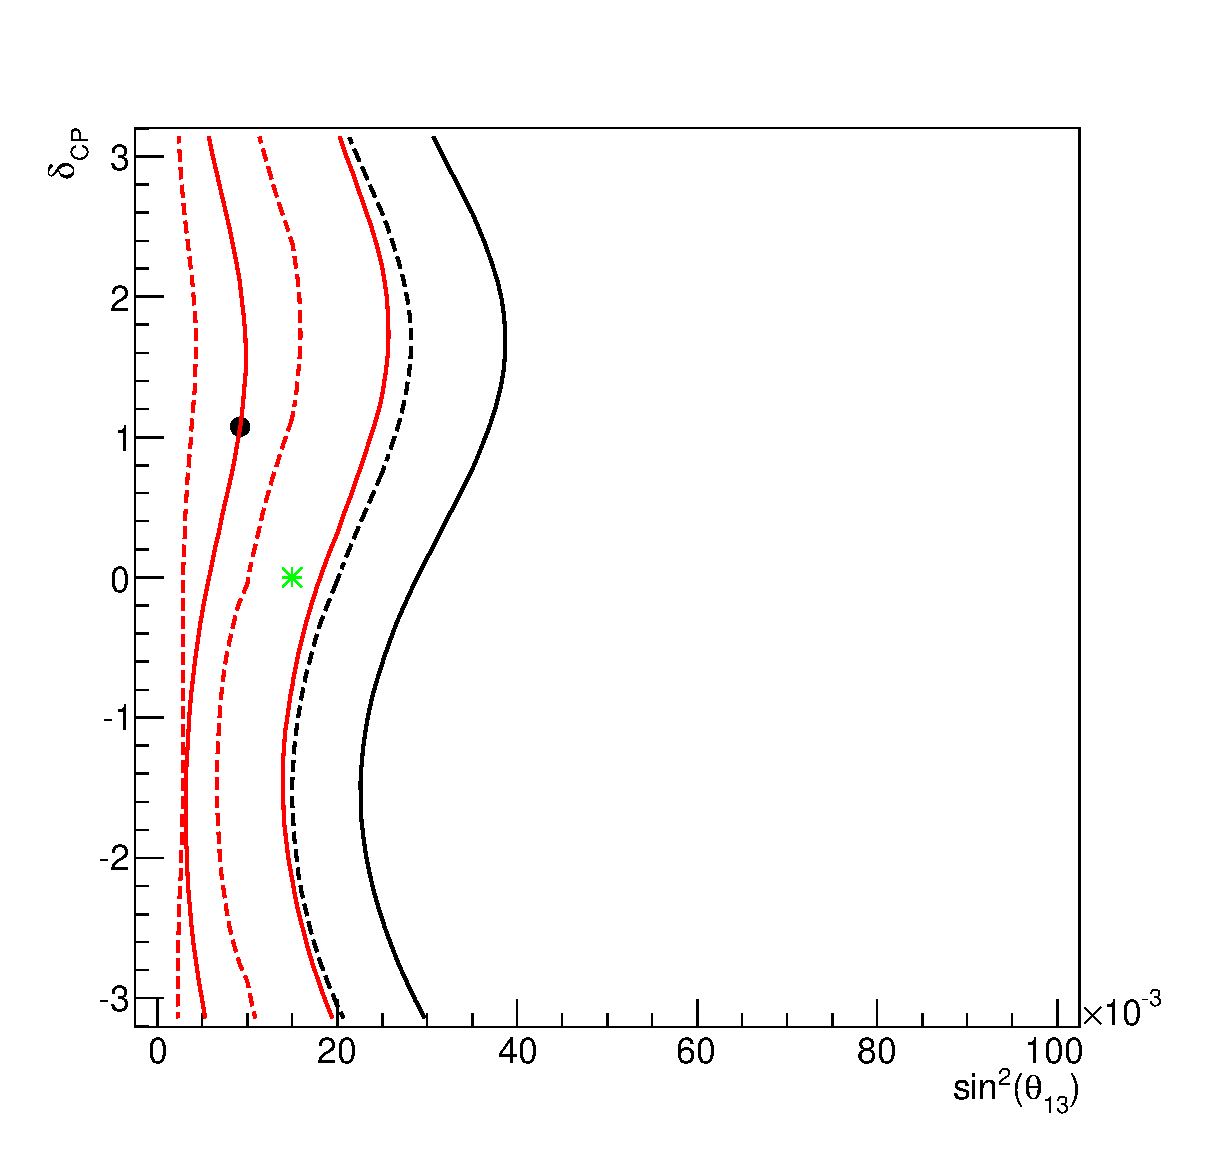
\includegraphics[width=15pc]{./images/appendix/fake_dataset_fits/realistic_fake_dataset3_chisq_theta13_deltacp_global_min.eps}
\caption {
  68\% and 90\% CL regions in ($sin^{2}\theta_{13}$, $\delta_{CP}$) space for fake dataset \#10.
  At each point, $\chi^2$ was minimized with respect to 
  $|\Delta m^{2}|$, $\sin^{2}\theta_{23}$
  and all relevant nuisance parameters for the joint analysis (black)
  and with respect to all relevant nuisance parameters for the appearance analysis (red).
  Notice that different methods are used to
  construct confidence regions for the joint analysis (global minimum) and for the 
  stand-alone appearance analysis (raster scan).
}
\label{fig:toymc10_confreg_sinsqtheta13_deltacp}
\end{minipage}
\hspace{0.03\linewidth}
\begin{minipage}[t]{0.48\linewidth}
\center
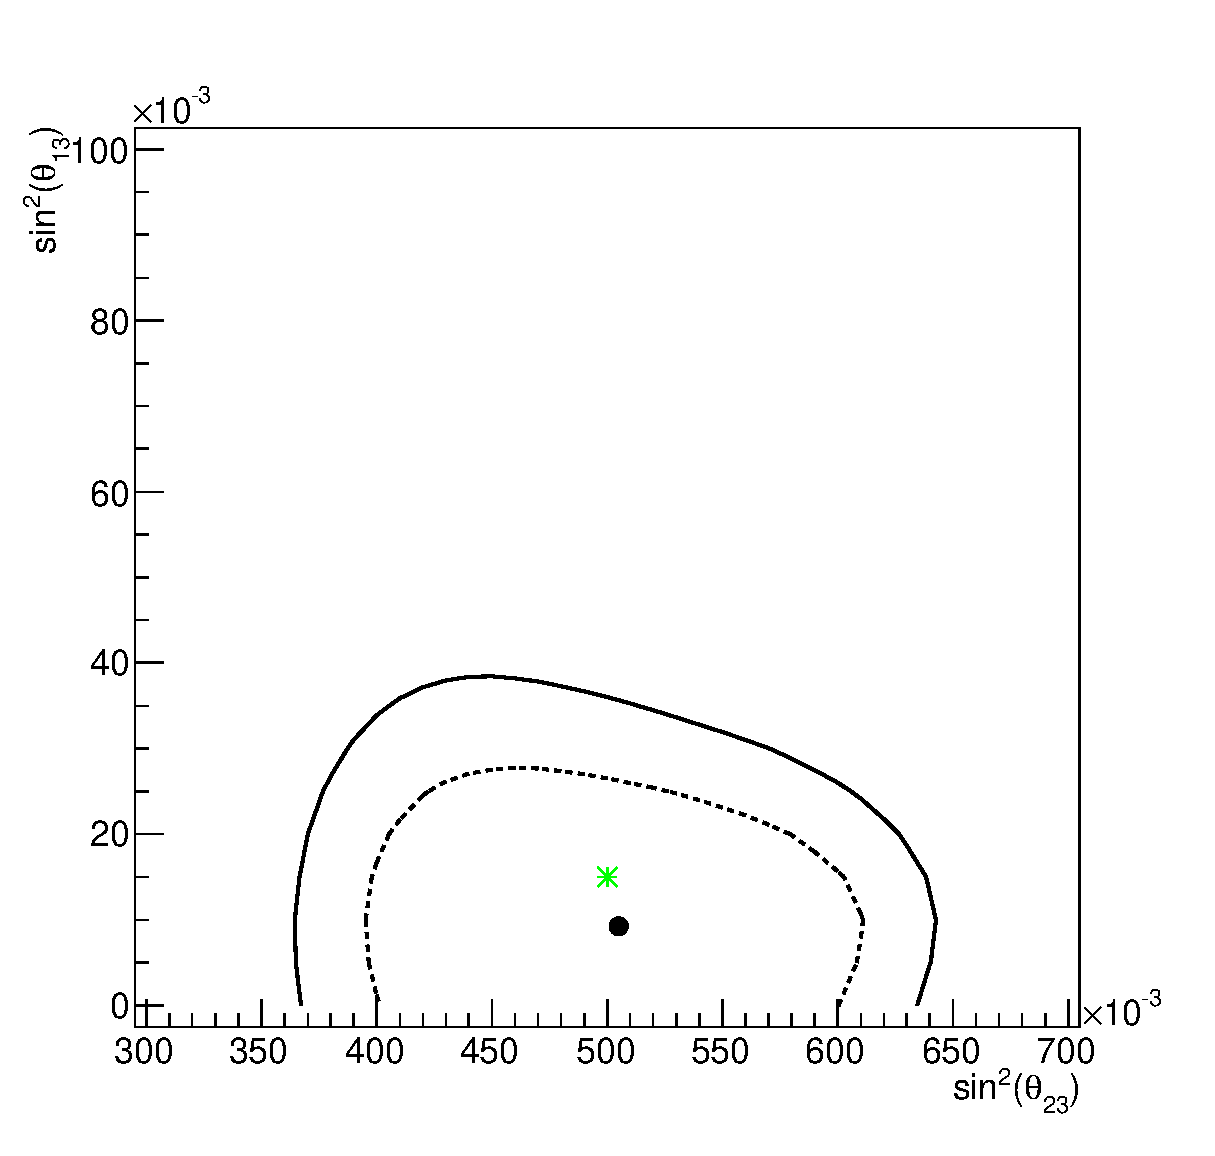
\includegraphics[width=15pc]{./images/appendix/fake_dataset_fits/realistic_fake_dataset3_chisq_theta13_theta23_global_min.eps}
\caption {
  68\% and 90\% CL regions in ($sin^{2}\theta_{23}$, $sin^{2}\theta_{13}$) space for fake dataset \#10.
  At each point, $\chi^2$ was minimized with respect to 
  all oscillation parameters not shown (and not considered to be fixed)
  and all relevant nuisance parameters.
}
\label{fig:toymc10_confreg_sinsqtheta23_sinsqtheta13}
\end{minipage}

\end{figure*}





% 
% 
% ..............................................
% Fake dataset #11
% 
%

\clearpage
\begin{figure*}[htb]

\begin{minipage}[t]{0.46\linewidth}
\center
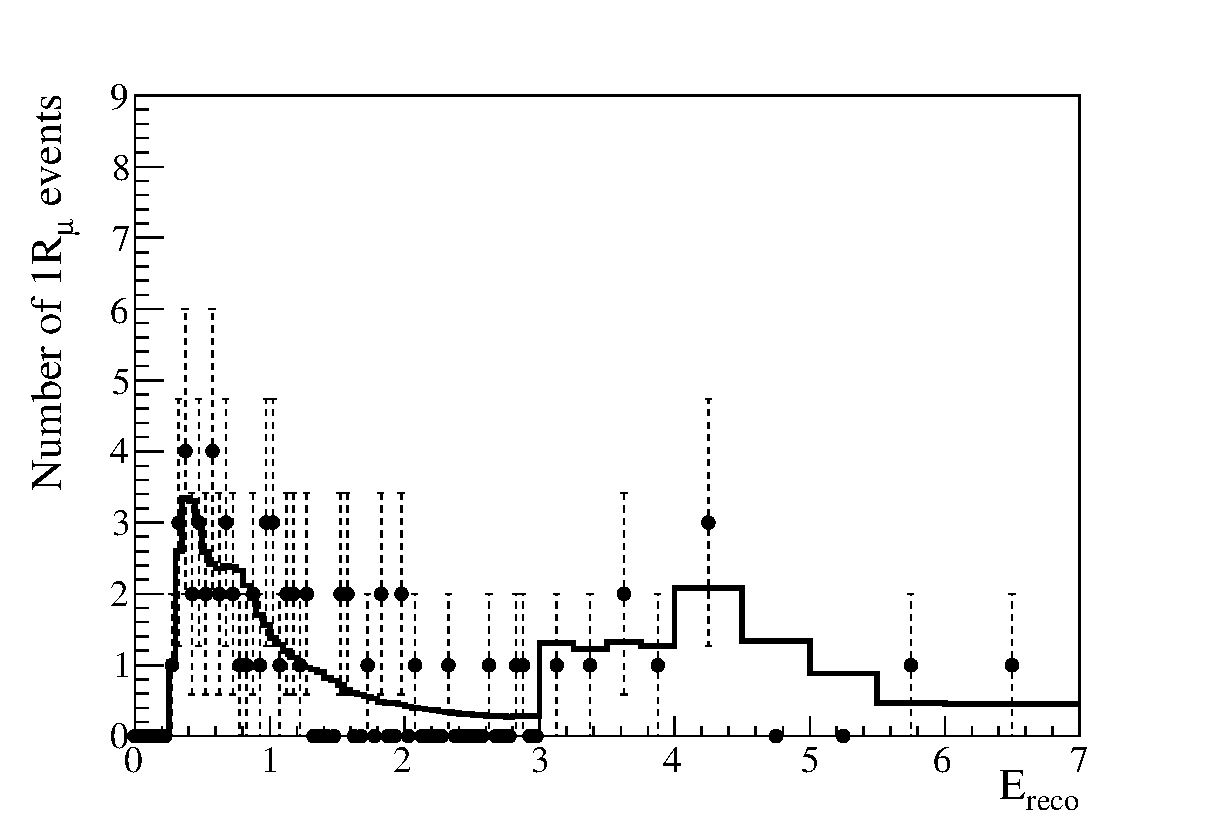
\includegraphics[width=15pc]{./images/appendix/fake_dataset_fits/realistic_fake_dataset4_nh_1st_1Rmu.eps}
\caption {
  Single $\mu$-like ring event best-fit reconstructed energy spectrum
  to fake dataset \#11.
}
\label{fig:toymc11_1Rmu_bestfit_spectrum}
\end{minipage}
\hspace{0.03\linewidth}
\begin{minipage}[t]{0.46\linewidth}
\center
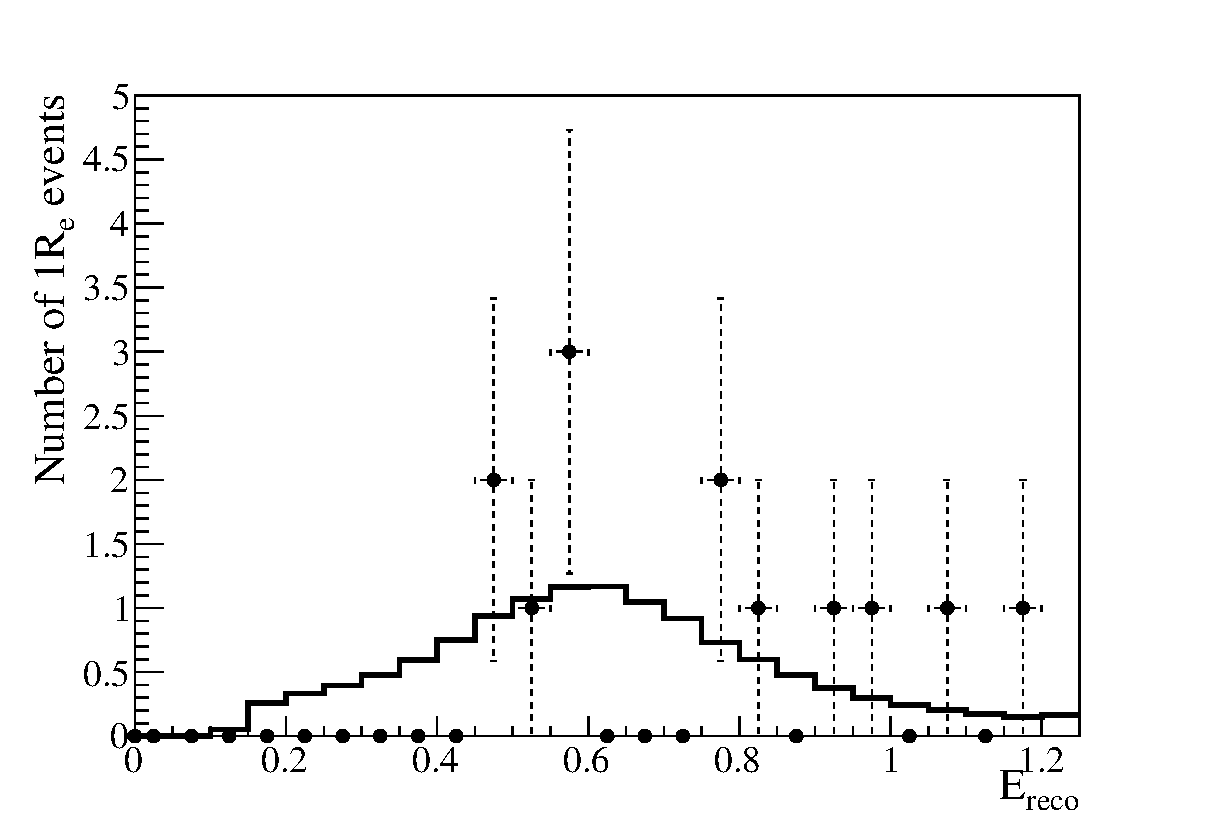
\includegraphics[width=15pc]{./images/appendix/fake_dataset_fits/realistic_fake_dataset4_nh_1st_1Re.eps}
\caption {
  Single e-like ring event best-fit reconstructed energy spectrum
  to fake dataset \#11.
}
\label{fig:toymc11_1Re_bestfit_spectrum}
\end{minipage}

\vfill
\vspace*{0.7cm}

\begin{minipage}[t]{0.90\linewidth}
\center
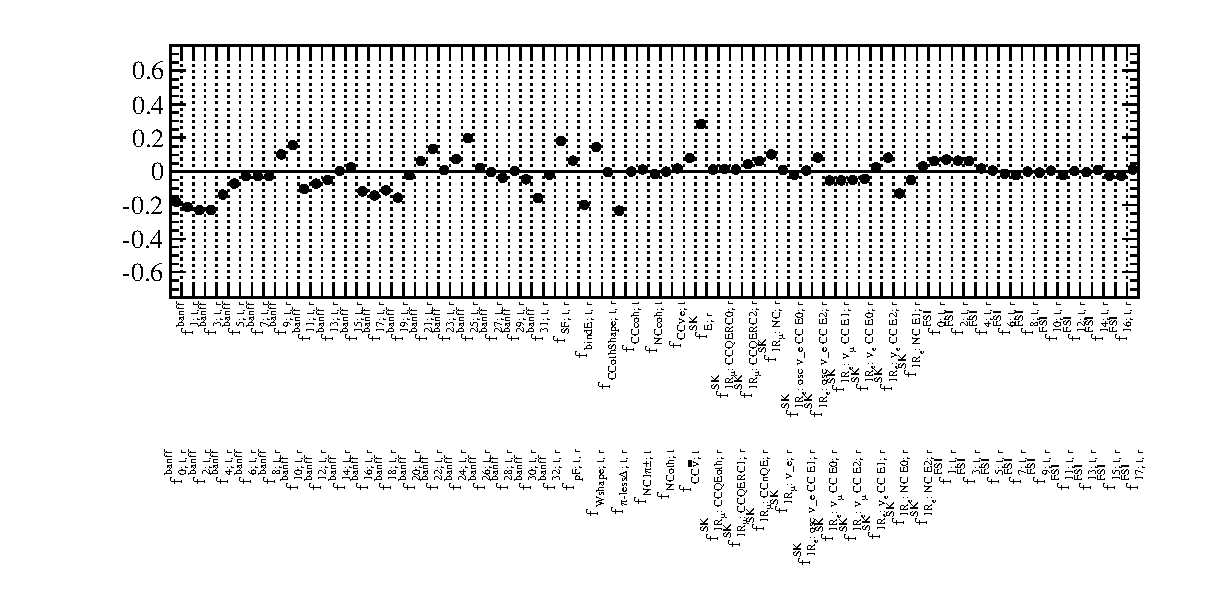
\includegraphics[width=30pc,angle=270]{./images/appendix/fake_dataset_fits/pulls_realistic_fake_dataset4_nh_1st.eps}
\caption {
  Systematic parameter pulls for the oscillation fit to fake dataset \#11.
}
\label{fig:toymc11_pulls}
\end{minipage}

\end{figure*}


%...........................................................
%
% chisq distributions used for calculating the fit p-values
%

\begin{figure*}[htb]

\begin{minipage}[t]{0.90\linewidth}
\center
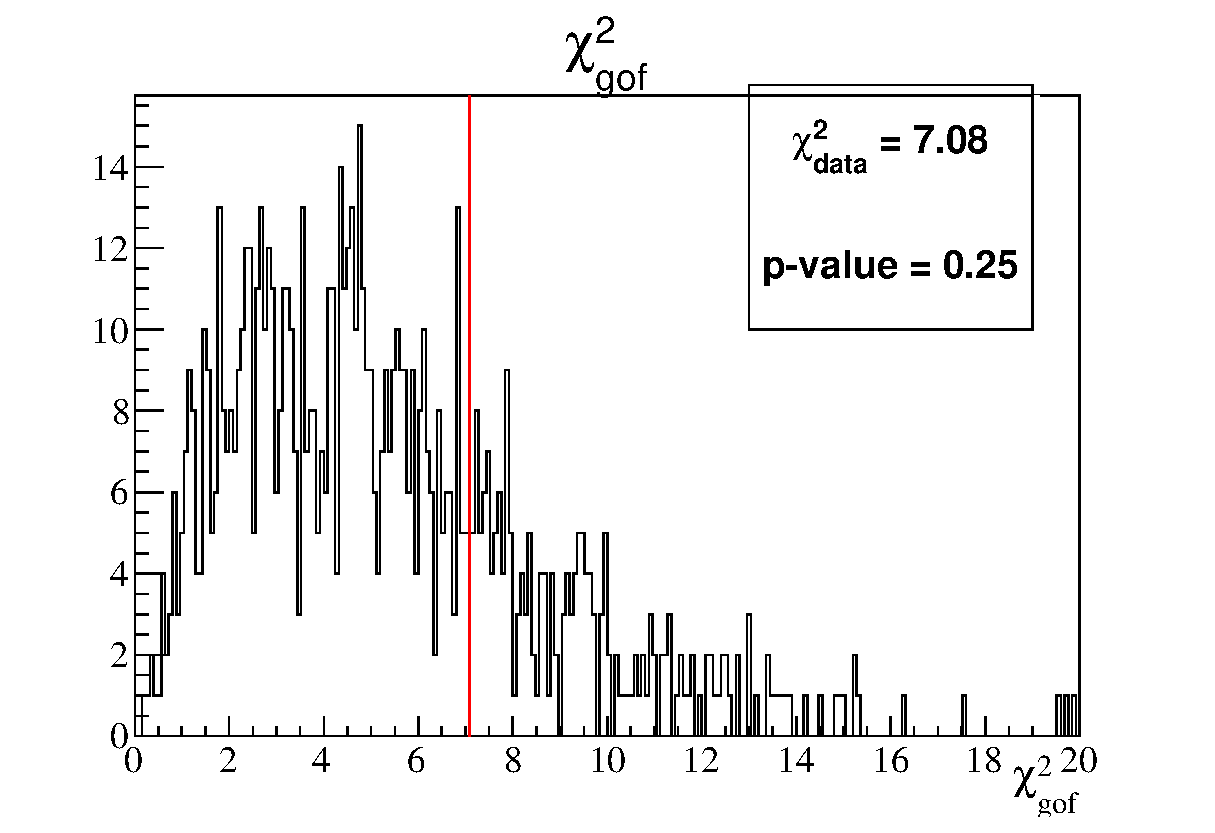
\includegraphics[width=30pc]{./images/appendix/fake_dataset_fits/realistic_fake_dataset4_nh_1st_gof_new.eps}
\caption {
  Distribution of $\chi^2_{gof}$, the goodness-of-fit (gof) $\chi^2$, 
  from 1k toy MC experiments generated at dataset \#11 joint 3-flavour analysis best-fit oscillation point.
  The $\chi^2_{gof}$ value for the dataset \#11 ($\chi^2_{data}$) is highlighted.
  All $\chi^2_{gof}$ values were computed 
  using the 5 (single $\mu$-like ring) + 3 (single e-like ring) 
  reconstructed energy binning scheme described in Sec.\ \ref{sec:goodness_of_fit}.
}
\label{fig:toymc11_gofchisq}
\end{minipage}

\vfill
\vspace*{0.7cm}

\begin{minipage}[t]{0.46\linewidth}
\center
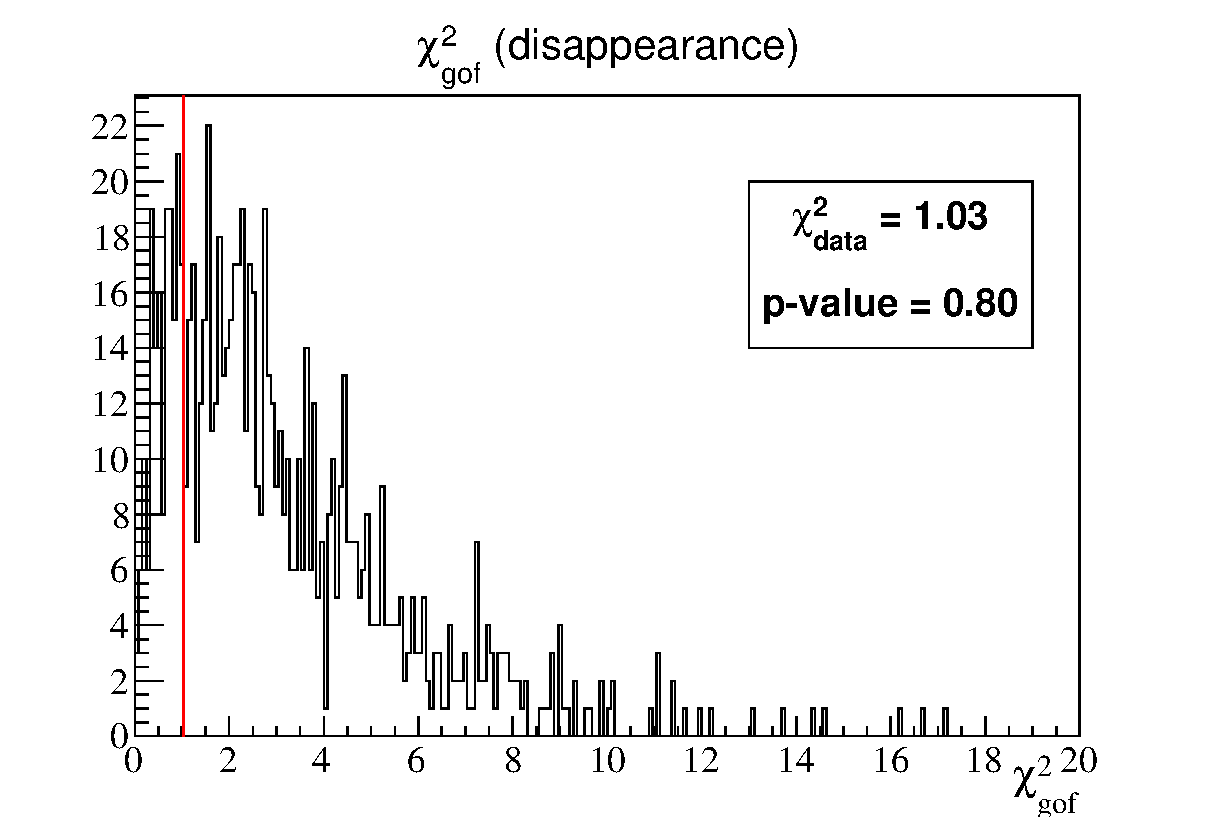
\includegraphics[width=18pc]{./images/appendix/fake_dataset_fits/realistic_fake_dataset4_nh_1st_gof_disap_new.eps}
\caption {
  Distribution of $\chi^2_{gof}$
  from 1k toy MC experiments generated at the dataset \#11 stand-alone 3-flavour $\nu_{\mu}$ disappearance analysis best-fit oscillation point.
  The $\chi^2_{gof}$ value for the dataset \#11 ($\chi^2_{data}$) is highlighted.
  All $\chi^2_{gof}$ values were computed 
  using the 5 (single $\mu$-like ring) 
  reconstructed energy binning scheme described in Sec.\ \ref{sec:goodness_of_fit}.
}
\label{fig:toymc11_gofchisq_disapp}
\end{minipage}
\hspace{0.03\linewidth}
\begin{minipage}[t]{0.46\linewidth}
\center
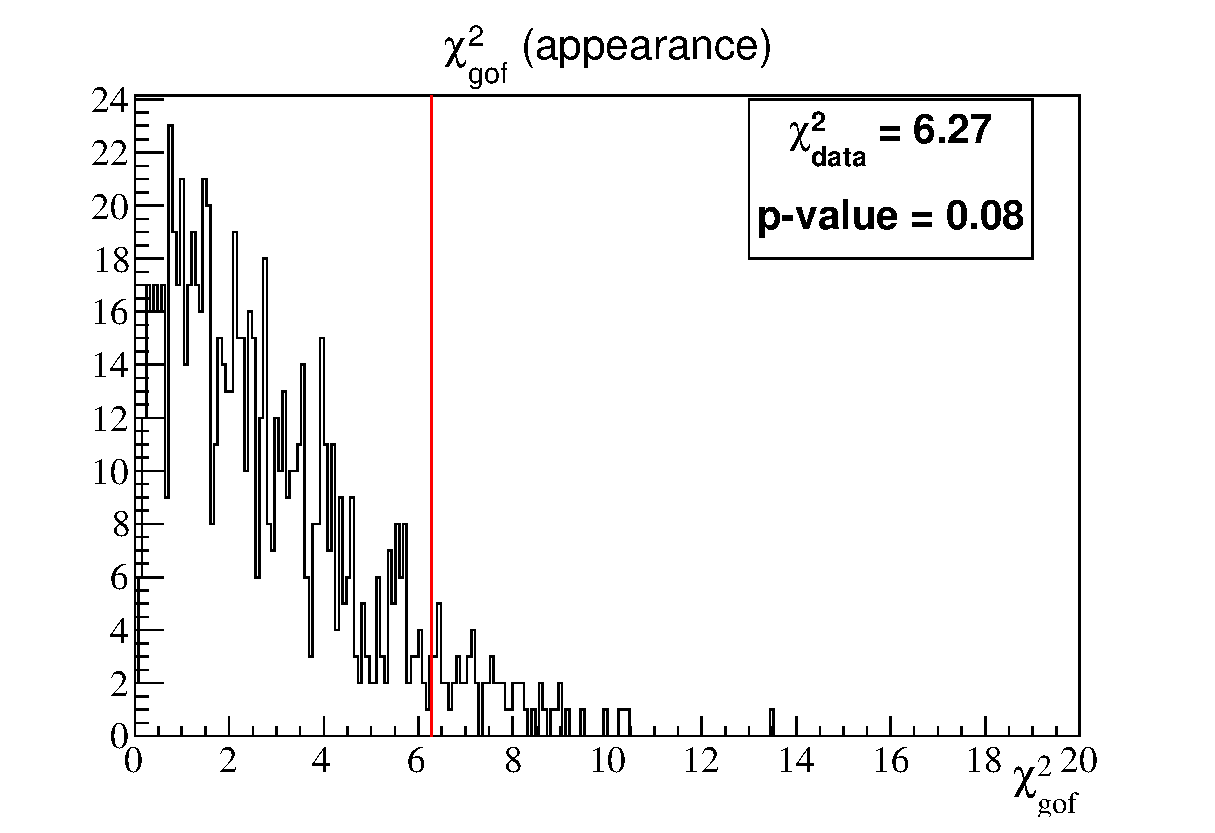
\includegraphics[width=18pc]{./images/appendix/fake_dataset_fits/realistic_fake_dataset4_nh_1st_gof_app_new.eps}
\caption {
  Distribution of $\chi^2_{gof}$
  from 1k toy MC experiments generated at the dataset \#11 stand-alone 3-flavour $\nu_{e}$ appearance analysis best-fit oscillation point.
  The $\chi^2_{gof}$ value for the dataset \#11 ($\chi^2_{data}$) is highlighted.
  All $\chi^2_{gof}$ values were computed 
  using the 3 (single e-like ring) 
  reconstructed energy binning scheme  as described in Sec.\ \ref{sec:goodness_of_fit}.
}
\label{fig:toymc11_gofchisq_app}
\end{minipage}

\end{figure*}



%
% delta\chisq and contours
%

\begin{figure*}[htb]

\begin{minipage}[t]{0.22\linewidth}
\center
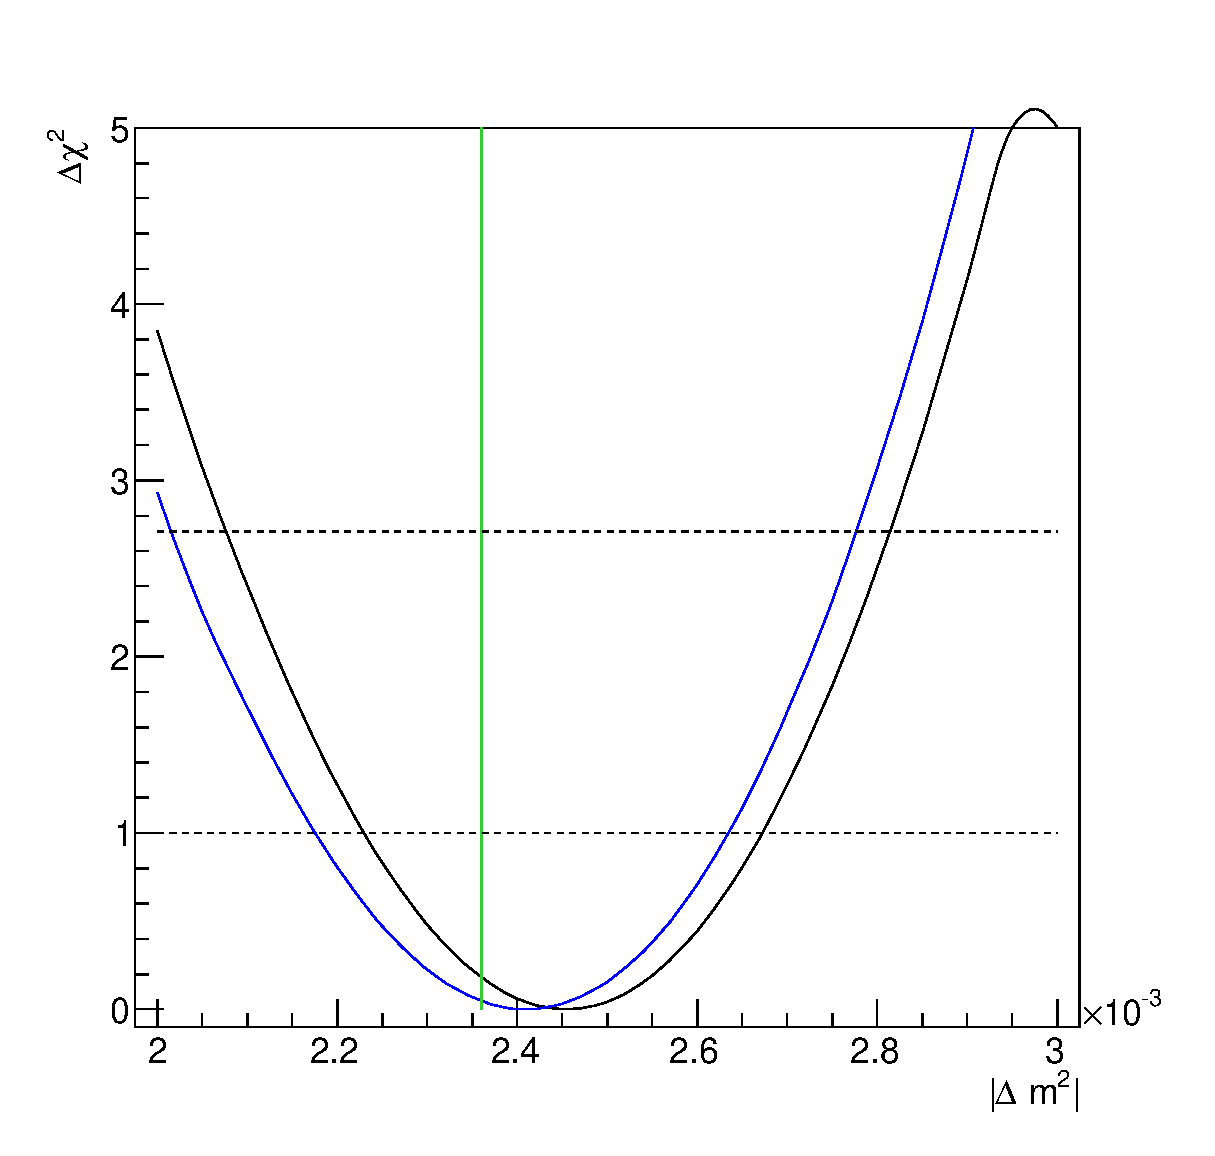
\includegraphics[width=9pc]{./images/appendix/fake_dataset_fits/realistic_fake_dataset4_chisq_dm23sq_global_min.eps}
\caption {
  $\Delta\chi^2$ as function of $|\Delta m^{2}|$ for fake dataset \#11.
  At each point, $\chi^2$ was minimized with respect to 
  $\sin^{2}\theta_{23}$, $\sin^{2}\theta_{13}$, $\delta_{CP}$
  and all relevant nuisance parameters for the joint analysis (black)
  and with respect to $\sin^{2}\theta_{23}$ and all relevant nuisance
  parameters for the disappearance analysis (blue).
}
\label{fig:toymc11_dchisq_Dmsq}
\end{minipage}
\hspace{0.02\linewidth}
\begin{minipage}[t]{0.22\linewidth}
\center
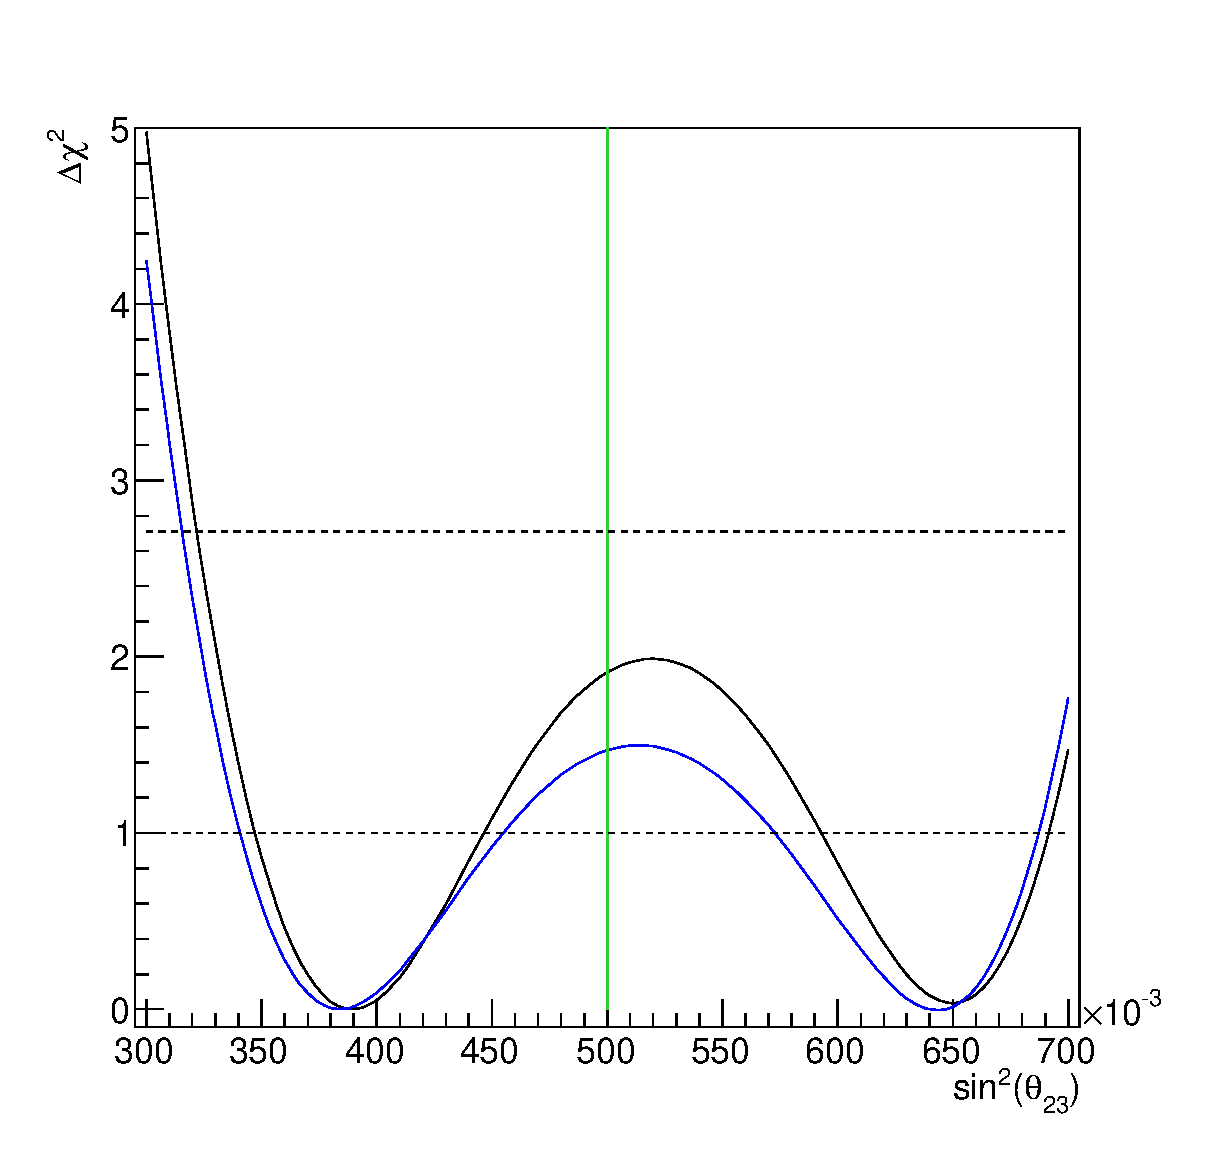
\includegraphics[width=9pc]{./images/appendix/fake_dataset_fits/realistic_fake_dataset4_chisq_theta23_global_min.eps}
\caption {
  $\Delta\chi^2$ as function of $sin^{2}\theta_{23}$ for fake dataset \#11.
  At each point, $\chi^2$ was minimized with respect to 
  $|\Delta m^{2}|$, $\sin^{2}\theta_{13}$, $\delta_{CP}$
  and all relevant nuisance parameters for the joint analysis (black)
  and with respect to $\sin^{2}\theta_{23}$ and all relevant nuisance
  parameters for the disappearance analysis (blue).
}
\label{fig:toymc11_dchisq_sinsqtheta23}
\end{minipage}
\hspace{0.02\linewidth}
\begin{minipage}[t]{0.22\linewidth}
\center
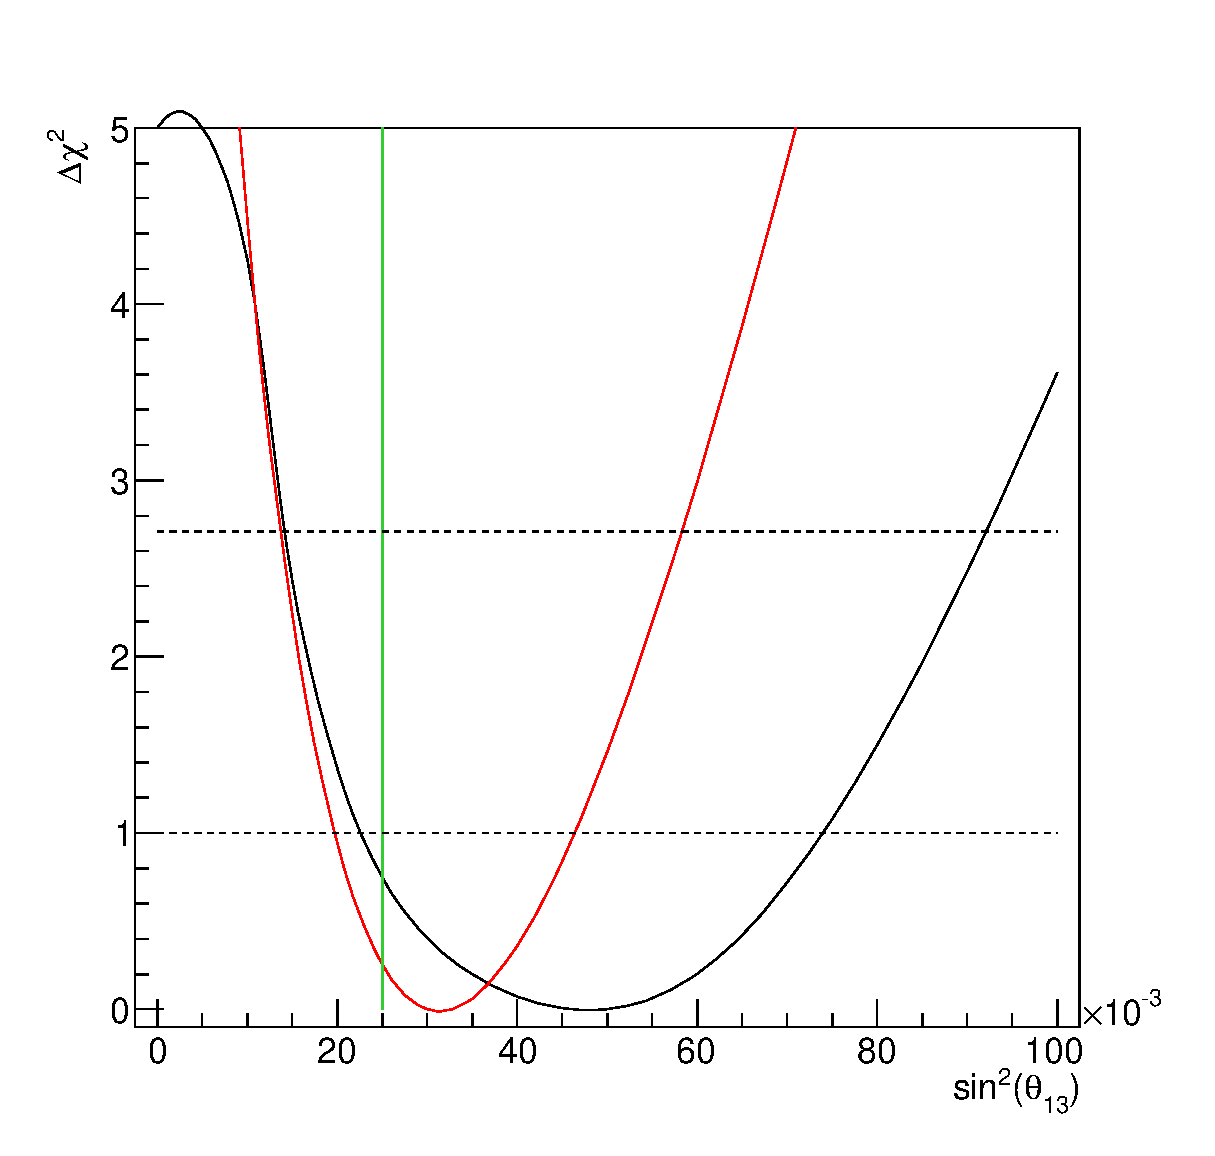
\includegraphics[width=9pc]{./images/appendix/fake_dataset_fits/realistic_fake_dataset4_chisq_theta13_global_min.eps}
\caption {
  $\Delta\chi^2$ as function of $sin^{2}\theta_{13}$ for fake dataset \#11.
  At each point, $\chi^2$ was minimized with respect to 
  $\sin^{2}\theta_{23}$, $\sin^{2}\theta_{13}$, $\delta_{CP}$
  and all relevant nuisance parameters for the joint analysis (black)
  and with respect to all relevant nuisance parameters 
  ($\delta_{CP}$ is fixed to 0) for the appearance analysis (red).
}
\label{fig:toymc11_dchisq_sinsqtheta13}
\end{minipage}
\hspace{0.02\linewidth}
\begin{minipage}[t]{0.22\linewidth}
\center
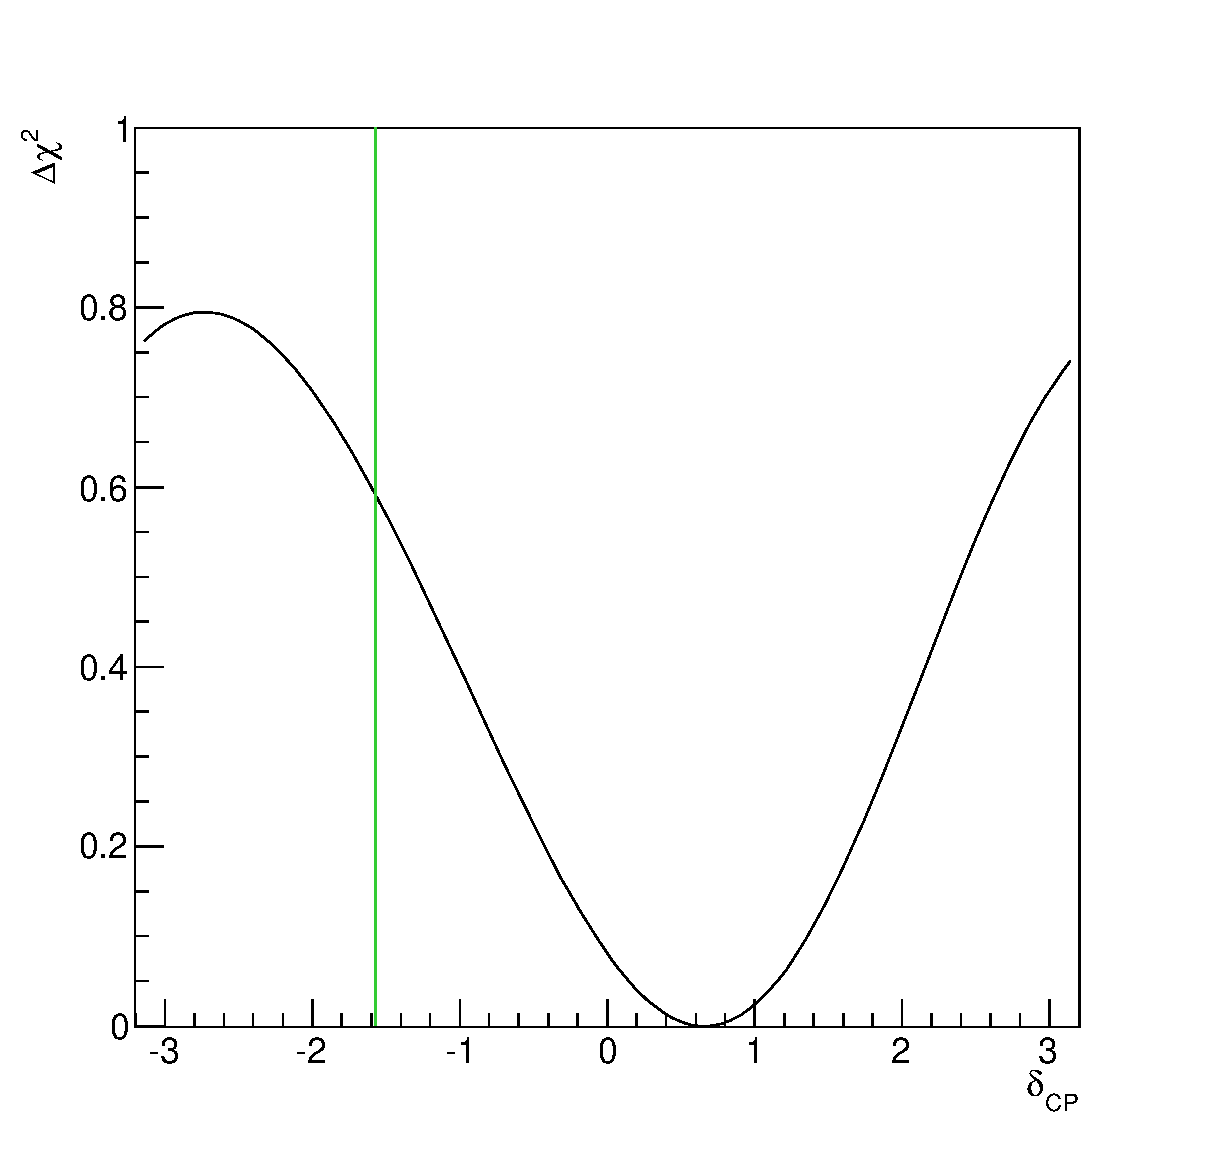
\includegraphics[width=9pc]{.//images/appendix/fake_dataset_fits/realistic_fake_dataset4_chisq_deltacp_global_min.eps}
\caption {
  $\Delta\chi^2$ as function of $\delta_{CP}$ for fake dataset \#11.
  At each point, $\chi^2$ was minimized with respect to 
  all oscillation parameters not shown (and not considered to be fixed)
  and all relevant nuisance parameters.
}
\label{fig:toymc11_dchisq_deltacp}
\end{minipage}
\vfill
\vspace*{0.7cm}
\begin{minipage}[t]{0.48\linewidth}
\center
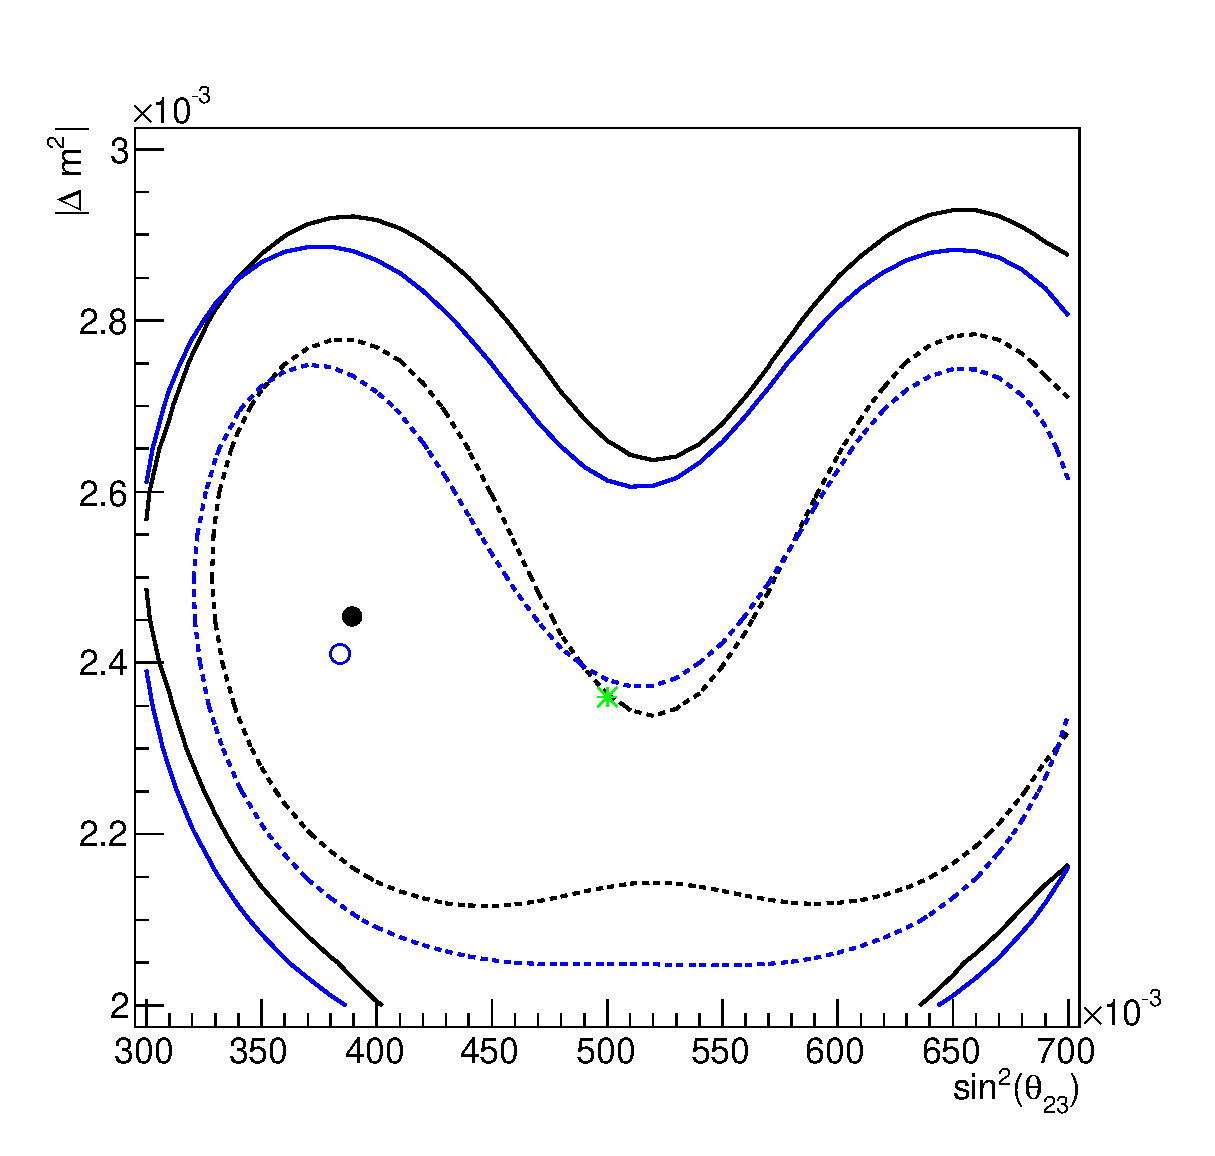
\includegraphics[width=15pc]{./images/appendix/fake_dataset_fits/realistic_fake_dataset4_chisq_theta23_dm23sq_global_min.eps}
\caption {
  68\% and 90\% CL regions in ($sin^{2}\theta_{23}$, $|\Delta m^{2}|$) space for fake dataset \#11.
  At each point, $\chi^2$ was minimized with respect to 
  $\sin^{2}\theta_{13}$, $\delta_{CP}$
  and all relevant nuisance parameters for the joint analysis (black)
  and with respect to all relevant nuisance parameters for the disappearance analysis (blue).
}
\label{fig:toymc11_confreg_sinsqtheta23_Dmsq}
\end{minipage}
\hspace{0.03\linewidth}
\begin{minipage}[t]{0.48\linewidth}
\center
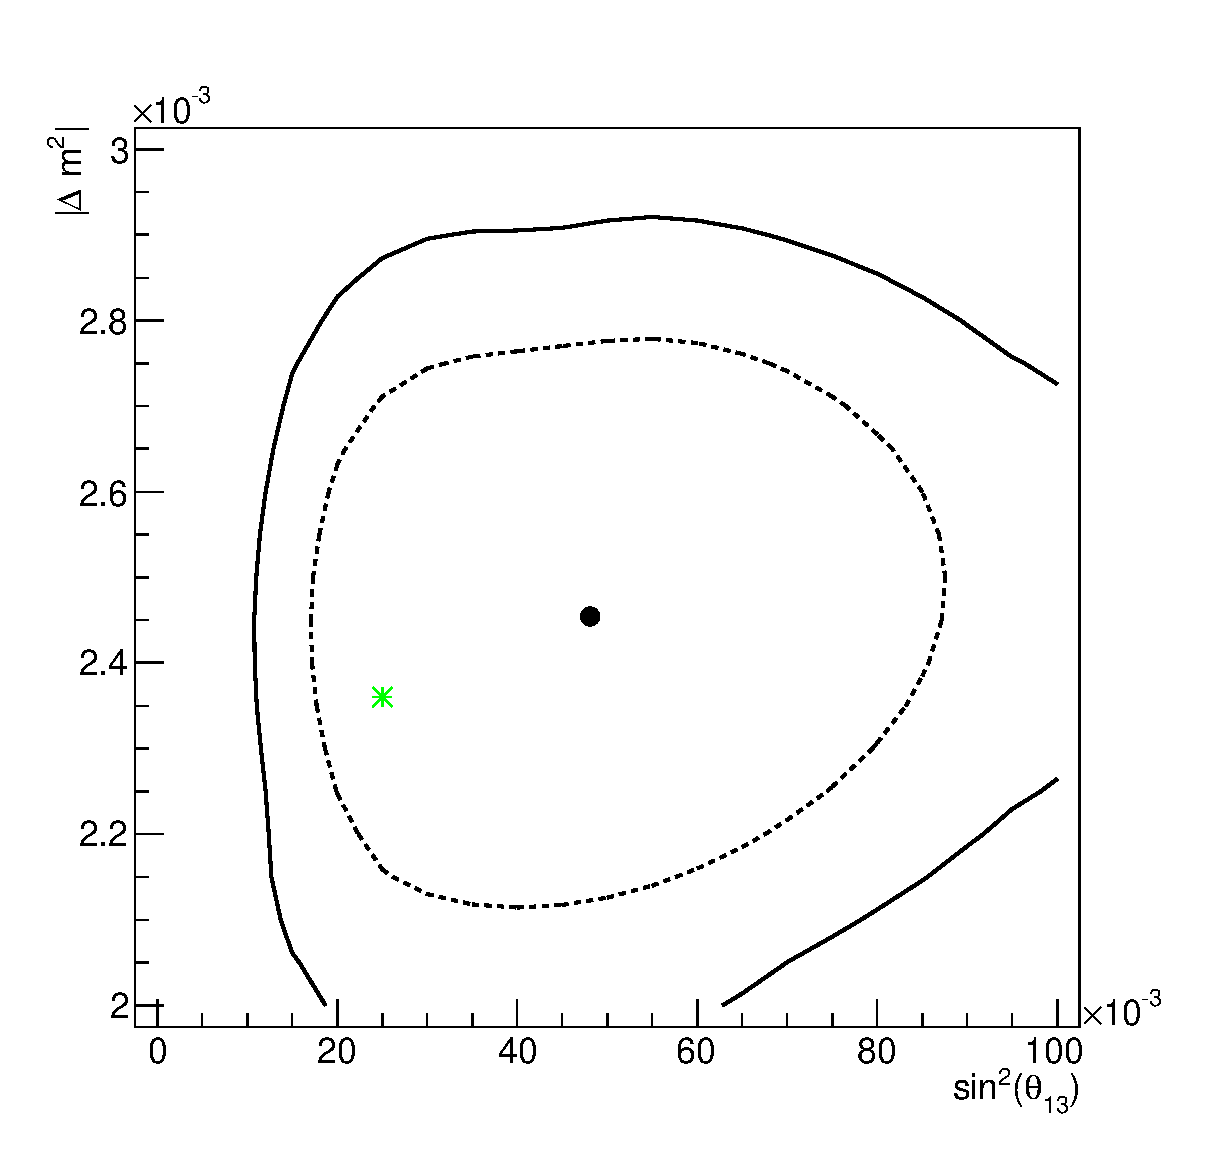
\includegraphics[width=15pc]{./images/appendix/fake_dataset_fits/realistic_fake_dataset4_chisq_theta13_dm23sq_global_min.eps}
\caption {
  68\% and 90\% CL regions in ($sin^{2}\theta_{13}$, $|\Delta m^{2}|$) space for fake dataset \#11.
  At each point, $\chi^2$ was minimized with respect to 
  all oscillation parameters not shown (and not considered to be fixed)
  and all relevant nuisance parameters.
}
\label{fig:toymc11_confreg_sinsqtheta13_Dmsq}
\end{minipage}

\vfill
\vspace*{0.7cm}

\begin{minipage}[t]{0.48\linewidth}
\center
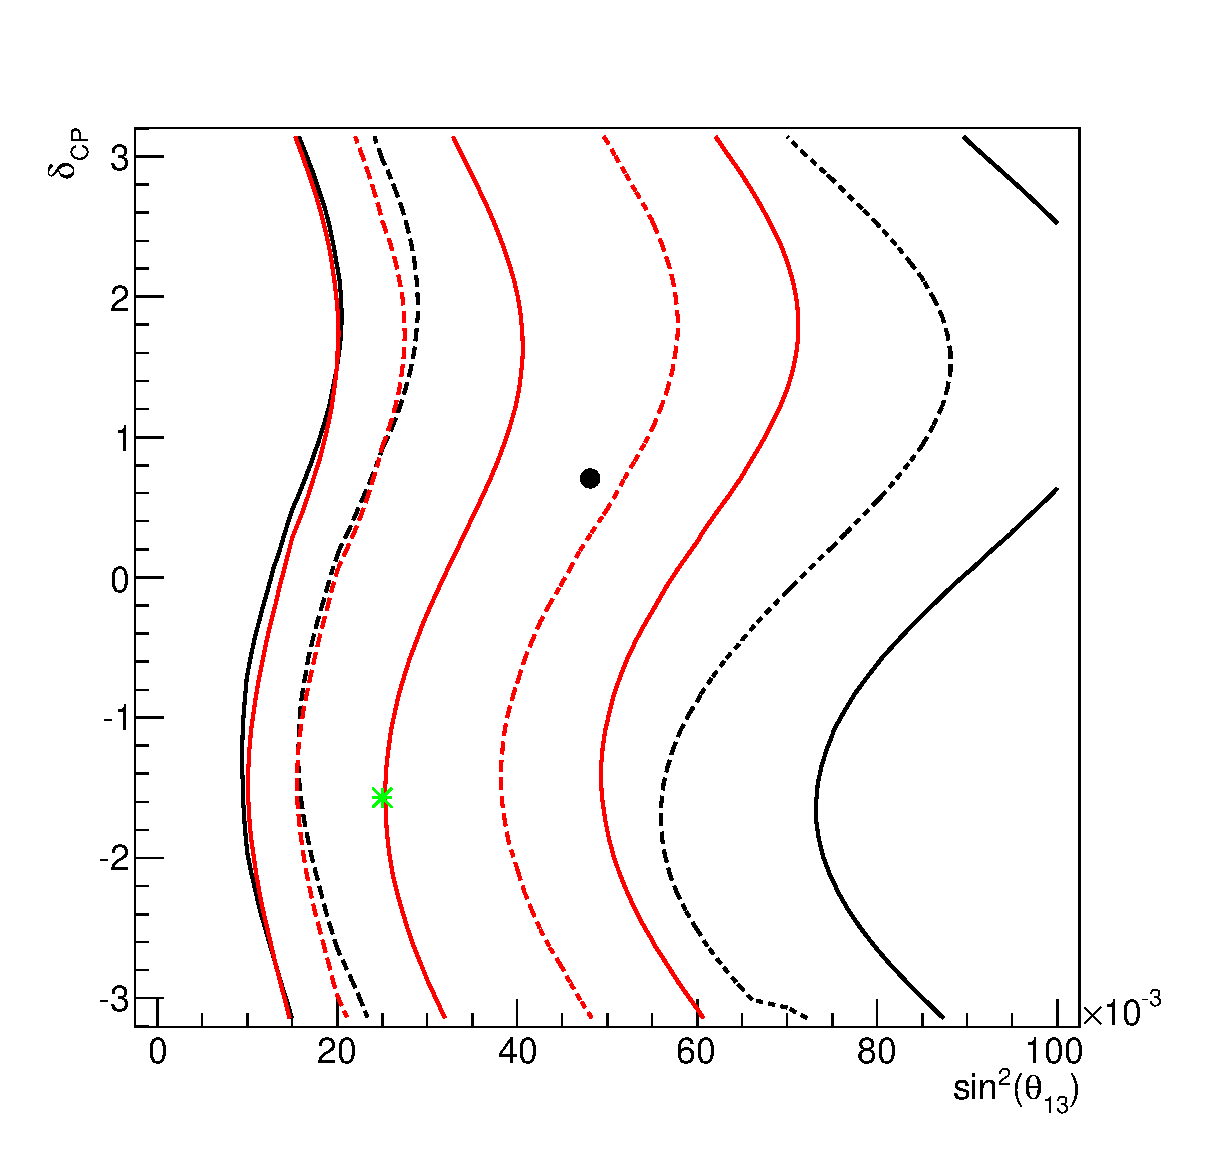
\includegraphics[width=15pc]{./images/appendix/fake_dataset_fits/realistic_fake_dataset4_chisq_theta13_deltacp_global_min.eps}
\caption {
  68\% and 90\% CL regions in ($sin^{2}\theta_{13}$, $\delta_{CP}$) space for fake dataset \#11.
  At each point, $\chi^2$ was minimized with respect to 
  $|\Delta m^{2}|$, $\sin^{2}\theta_{23}$
  and all relevant nuisance parameters for the joint analysis (black)
  and with respect to all relevant nuisance parameters for the appearance analysis (red).
  Notice that different methods are used to
  construct confidence regions for the joint analysis (global minimum) and for the 
  stand-alone appearance analysis (raster scan).
}
\label{fig:toymc11_confreg_sinsqtheta13_deltacp}
\end{minipage}
\hspace{0.03\linewidth}
\begin{minipage}[t]{0.48\linewidth}
\center
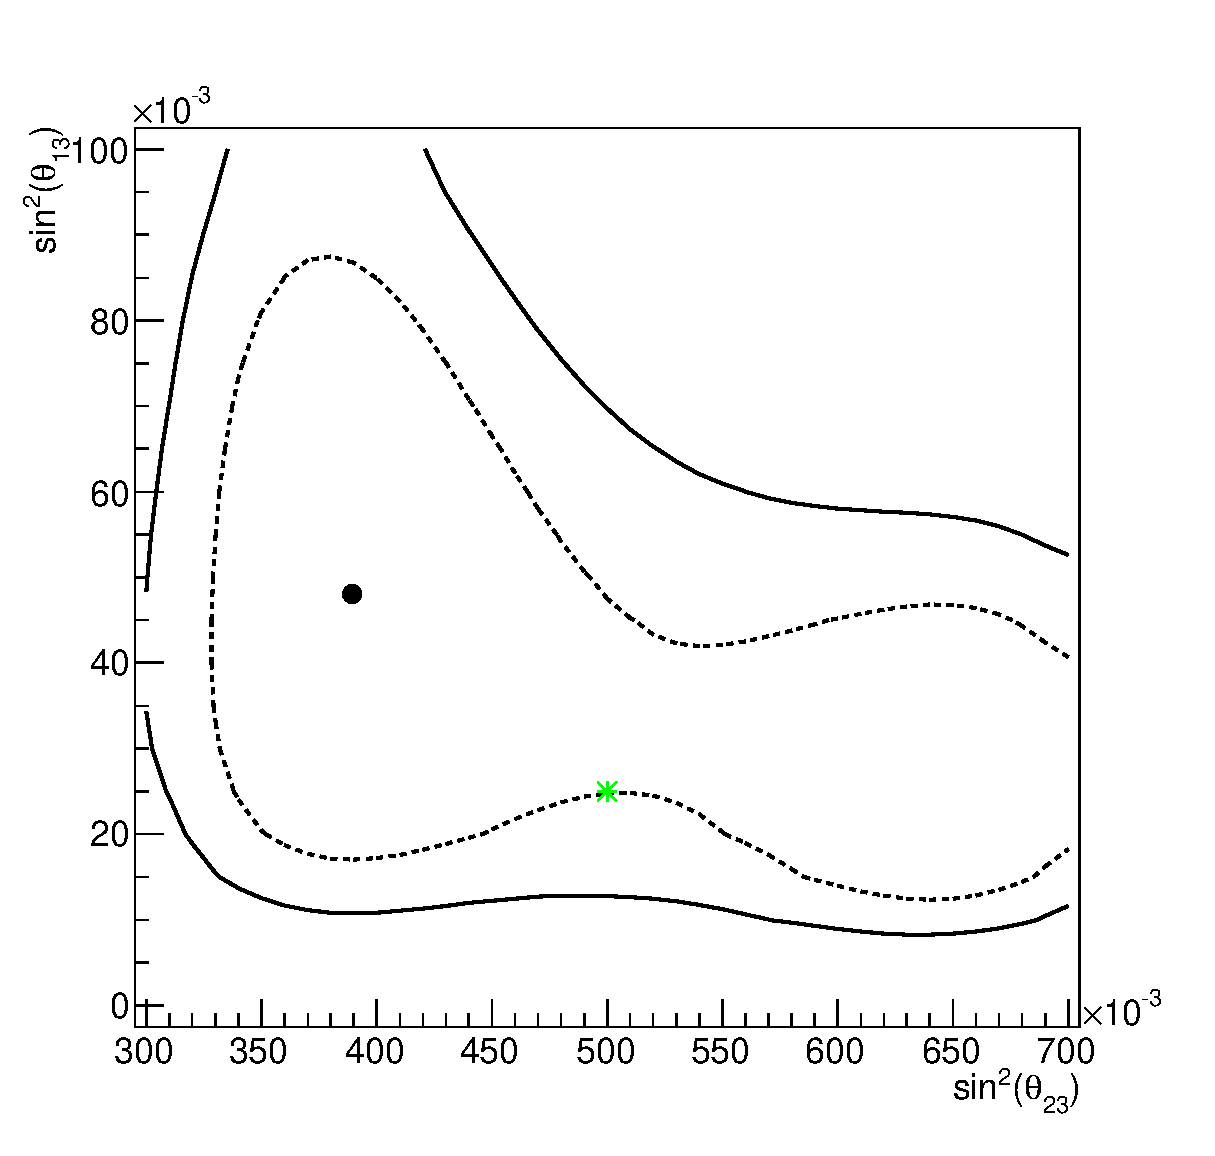
\includegraphics[width=15pc]{./images/appendix/fake_dataset_fits/realistic_fake_dataset4_chisq_theta13_theta23_global_min.eps}
\caption {
  68\% and 90\% CL regions in ($sin^{2}\theta_{23}$, $sin^{2}\theta_{13}$) space for fake dataset \#11.
  At each point, $\chi^2$ was minimized with respect to 
  all oscillation parameters not shown (and not considered to be fixed)
  and all relevant nuisance parameters.
}
\label{fig:toymc11_confreg_sinsqtheta23_sinsqtheta13}
\end{minipage}

\end{figure*}



% 
% 
% ..............................................
% Fake dataset #12
% 
%

\clearpage
\begin{figure*}[htb]

\begin{minipage}[t]{0.46\linewidth}
\center
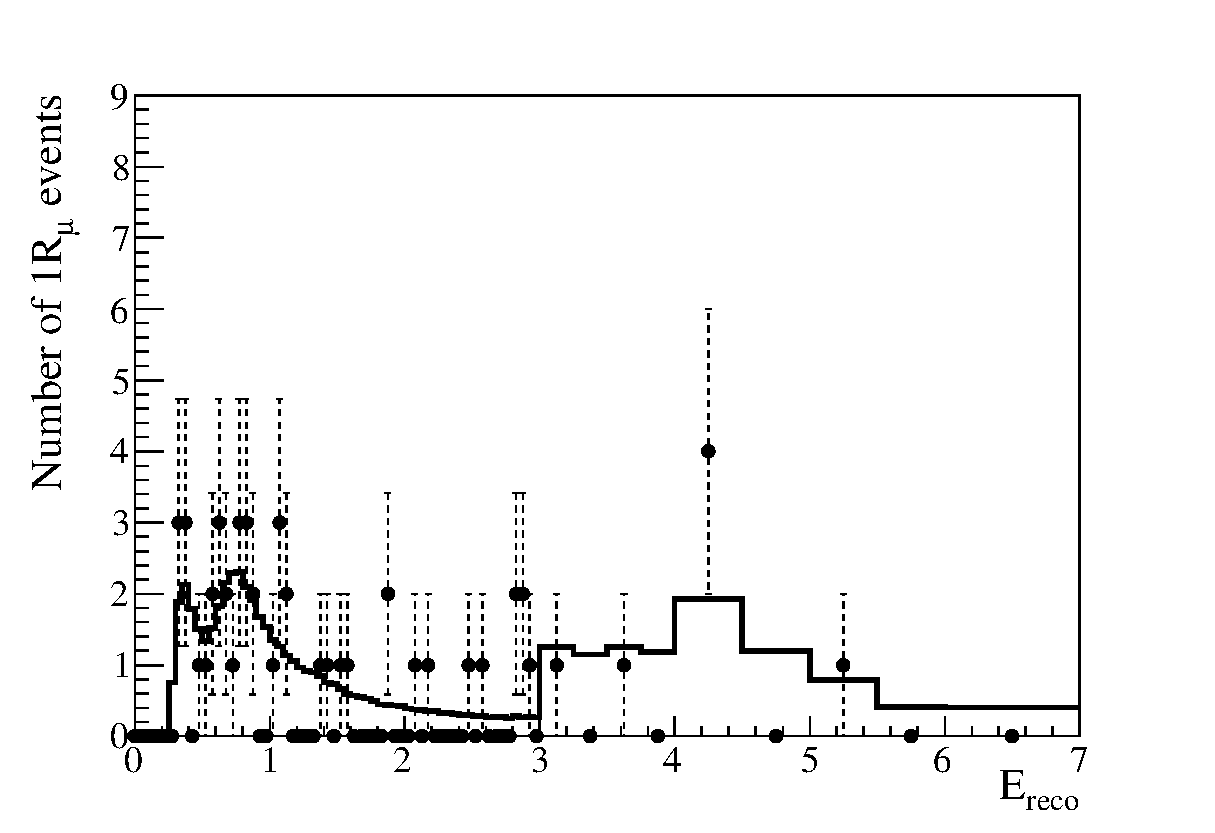
\includegraphics[width=15pc]{./images/appendix/fake_dataset_fits/realistic_fake_dataset5_nh_1st_1Rmu.eps}
\caption {
  Single $\mu$-like ring event best-fit reconstructed energy spectrum
  to fake dataset \#12.
}
\label{fig:toymc12_1Rmu_bestfit_spectrum}
\end{minipage}
\hspace{0.03\linewidth}
\begin{minipage}[t]{0.46\linewidth}
\center
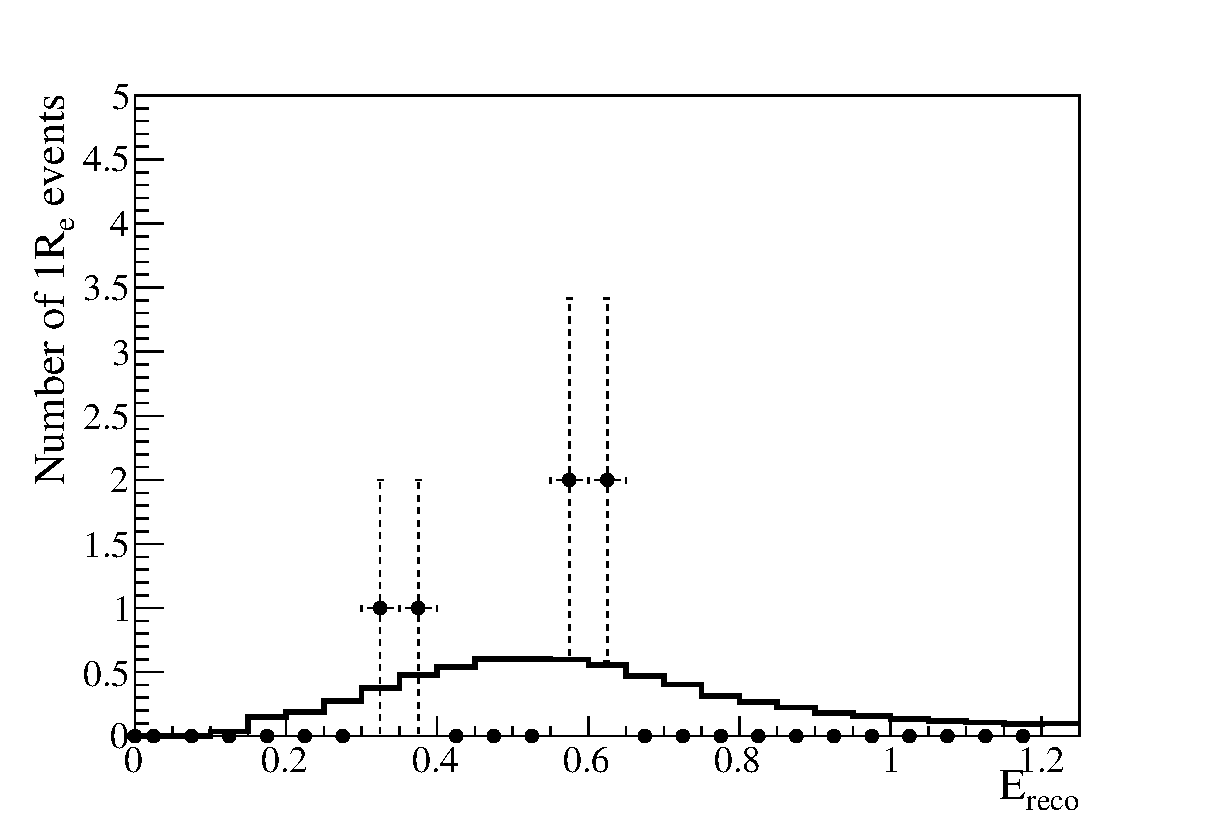
\includegraphics[width=15pc]{./images/appendix/fake_dataset_fits/realistic_fake_dataset5_nh_1st_1Re.eps}
\caption {
  Single e-like ring event best-fit reconstructed energy spectrum
  to fake dataset \#12.
}
\label{fig:toymc12_1Re_bestfit_spectrum}
\end{minipage}

\vfill
\vspace*{0.7cm}

\begin{minipage}[t]{0.90\linewidth}
\center
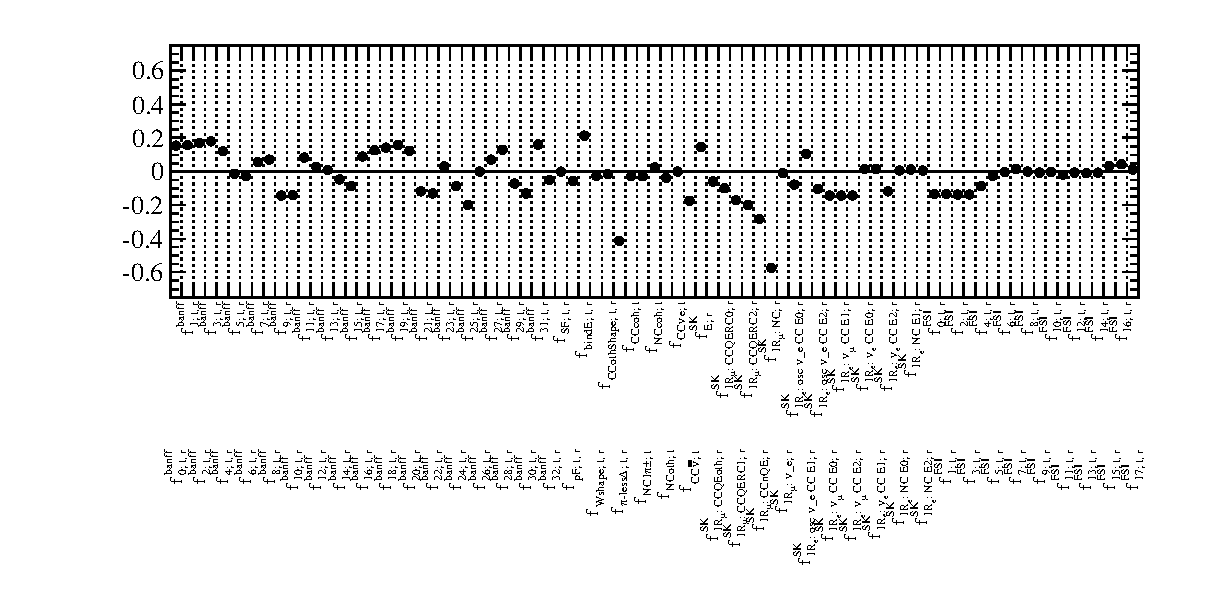
\includegraphics[width=30pc,angle=270]{./images/appendix/fake_dataset_fits/pulls_realistic_fake_dataset5_nh_1st.eps}
\caption {
  Systematic parameter pulls for the oscillation fit to fake dataset \#12.
}
\label{fig:toymc12_pulls}
\end{minipage}

\end{figure*}


%...........................................................
%
% chisq distributions used for calculating the fit p-values
%

\begin{figure*}[htb]

\begin{minipage}[t]{0.90\linewidth}
\center
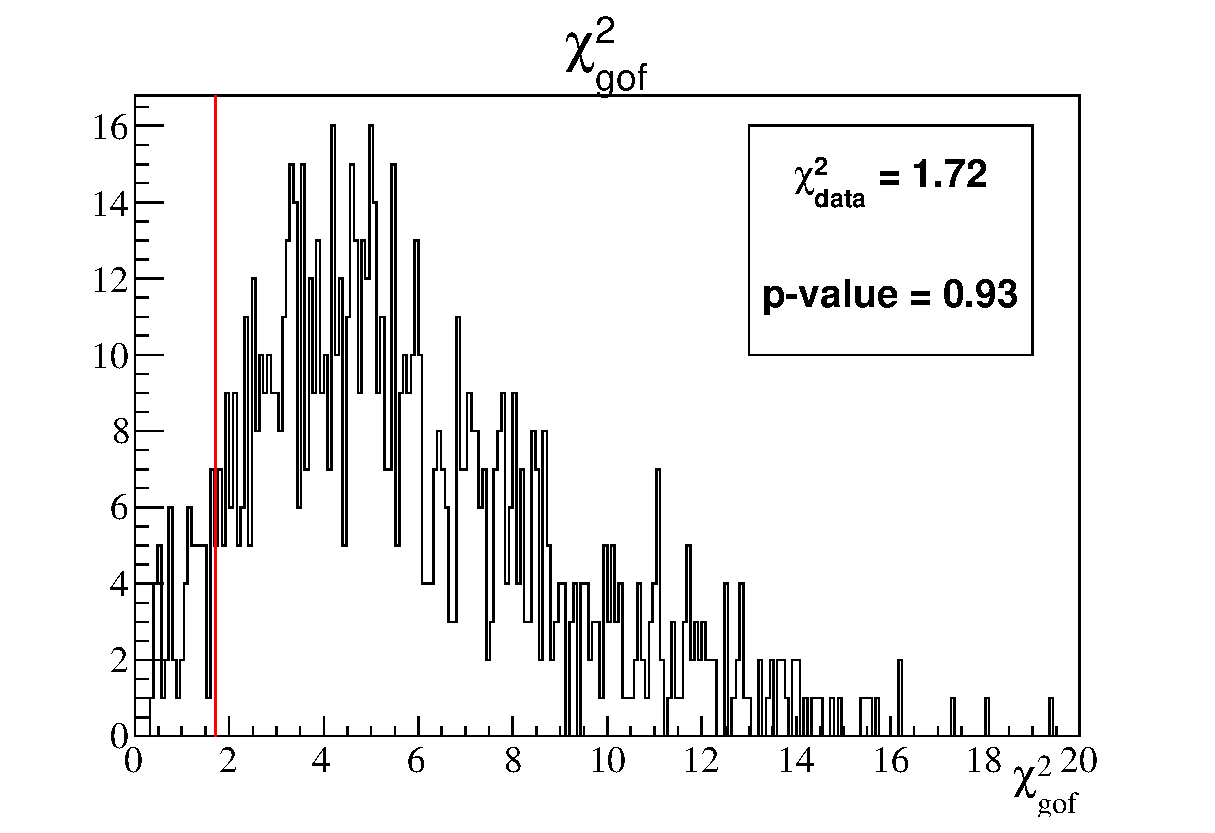
\includegraphics[width=30pc]{./images/appendix/fake_dataset_fits/realistic_fake_dataset5_nh_1st_gof_new.eps}
\caption {
  Distribution of $\chi^2_{gof}$, the goodness-of-fit (gof) $\chi^2$, 
  from 1k toy MC experiments generated at dataset \#12 joint 3-flavour analysis best-fit oscillation point.
  The $\chi^2_{gof}$ value for the dataset \#12 ($\chi^2_{data}$) is highlighted.
  All $\chi^2_{gof}$ values were computed 
  using the 5 (single $\mu$-like ring) + 3 (single e-like ring) 
  reconstructed energy binning scheme described in Sec.\ \ref{sec:goodness_of_fit}.
}
\label{fig:toymc12_gofchisq}
\end{minipage}

\vfill
\vspace*{0.7cm}

\begin{minipage}[t]{0.46\linewidth}
\center
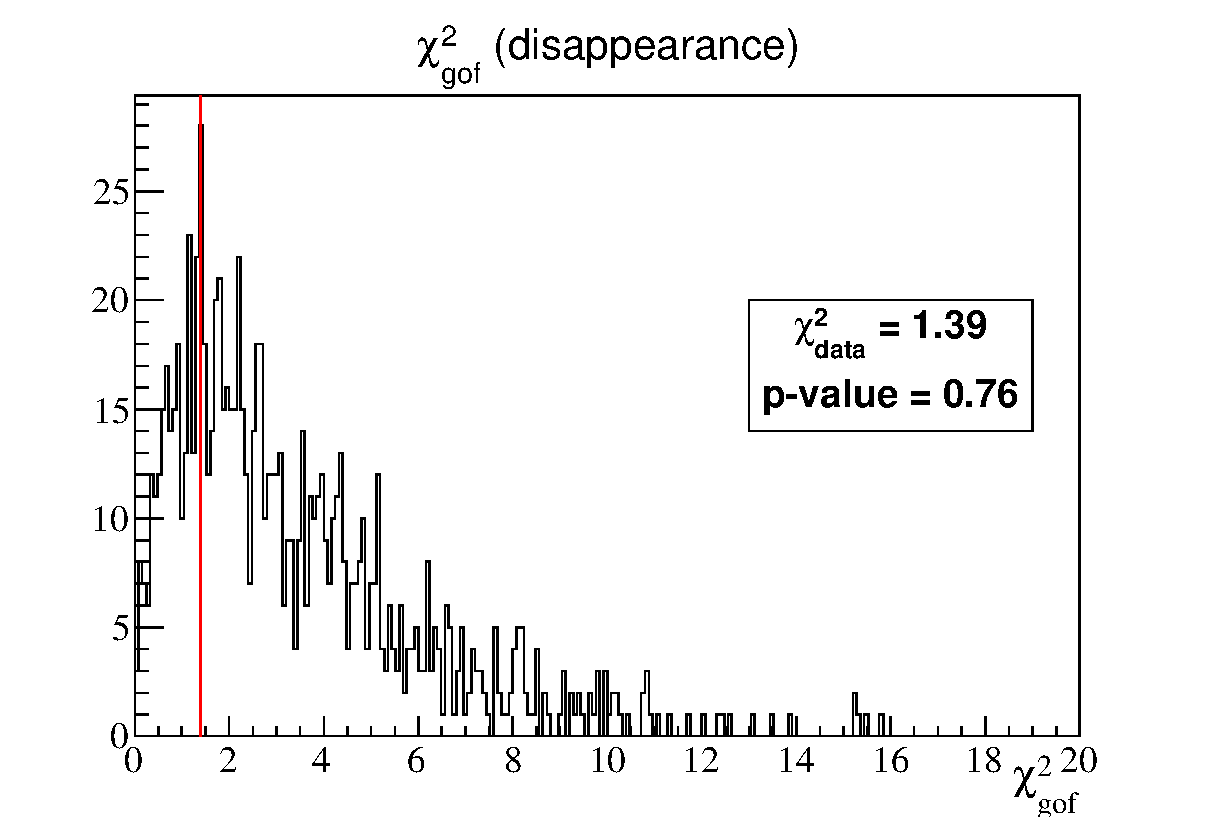
\includegraphics[width=18pc]{./images/appendix/fake_dataset_fits/realistic_fake_dataset5_nh_1st_gof_disap_new.eps}
\caption {
  Distribution of $\chi^2_{gof}$
  from 1k toy MC experiments generated at the dataset \#12 stand-alone 3-flavour $\nu_{\mu}$ disappearance analysis best-fit oscillation point.
  The $\chi^2_{gof}$ value for the dataset \#12 ($\chi^2_{data}$) is highlighted.
  All $\chi^2_{gof}$ values were computed 
  using the 5 (single $\mu$-like ring) 
  reconstructed energy binning scheme described in Sec.\ \ref{sec:goodness_of_fit}.
}
\label{fig:toymc12_gofchisq_disapp}
\end{minipage}
\hspace{0.03\linewidth}
\begin{minipage}[t]{0.46\linewidth}
\center
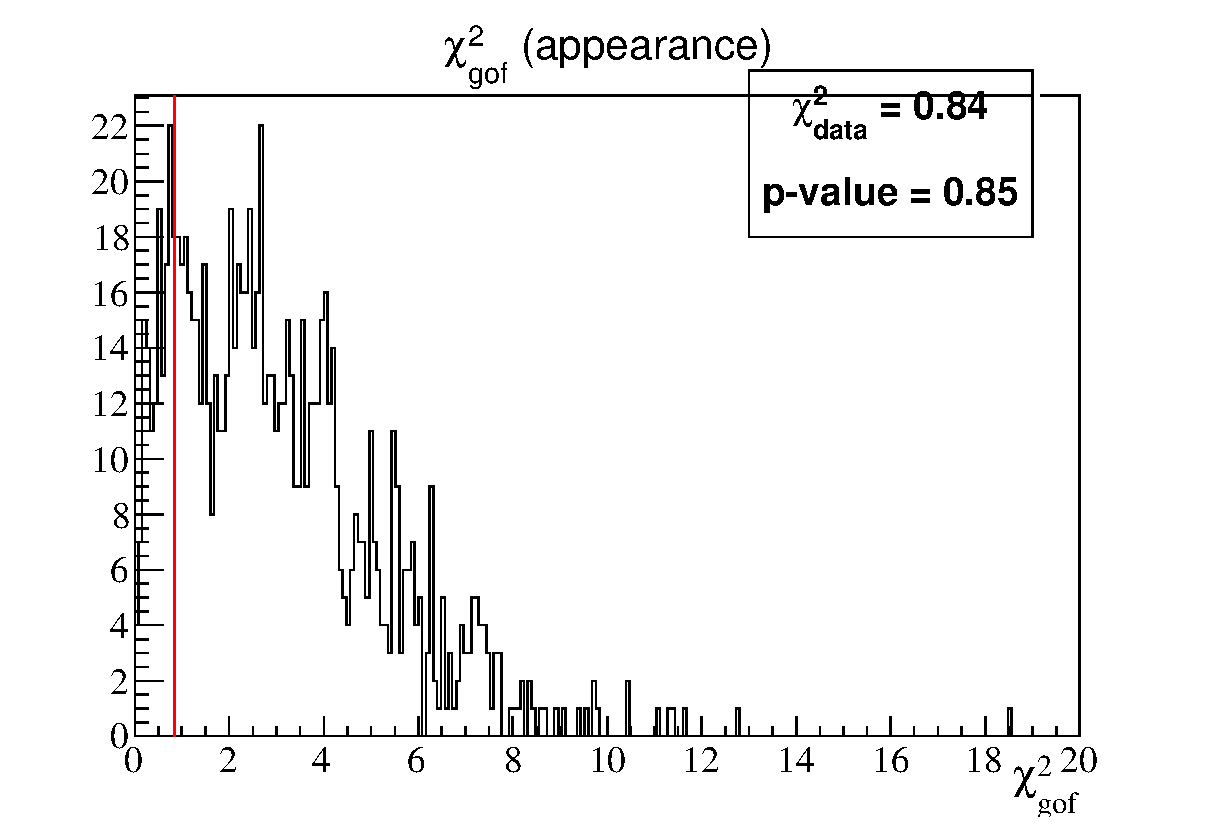
\includegraphics[width=18pc]{./images/appendix/fake_dataset_fits/realistic_fake_dataset5_nh_1st_gof_app_new.eps}
\caption {
  Distribution of $\chi^2_{gof}$
  from 1k toy MC experiments generated at the dataset \#12 stand-alone 3-flavour $\nu_{e}$ appearance analysis best-fit oscillation point.
  The $\chi^2_{gof}$ value for the dataset \#12 ($\chi^2_{data}$) is highlighted.
   All $\chi^2_{gof}$ values were computed 
  using the 3 (single e-like ring) 
  reconstructed energy binning scheme  as described in Sec.\ \ref{sec:goodness_of_fit}.
}
\label{fig:toymc12_gofchisq_app}
\end{minipage}

\end{figure*}



%
% delta\chisq and contours
%

\begin{figure*}[htb]

\begin{minipage}[t]{0.22\linewidth}
\center
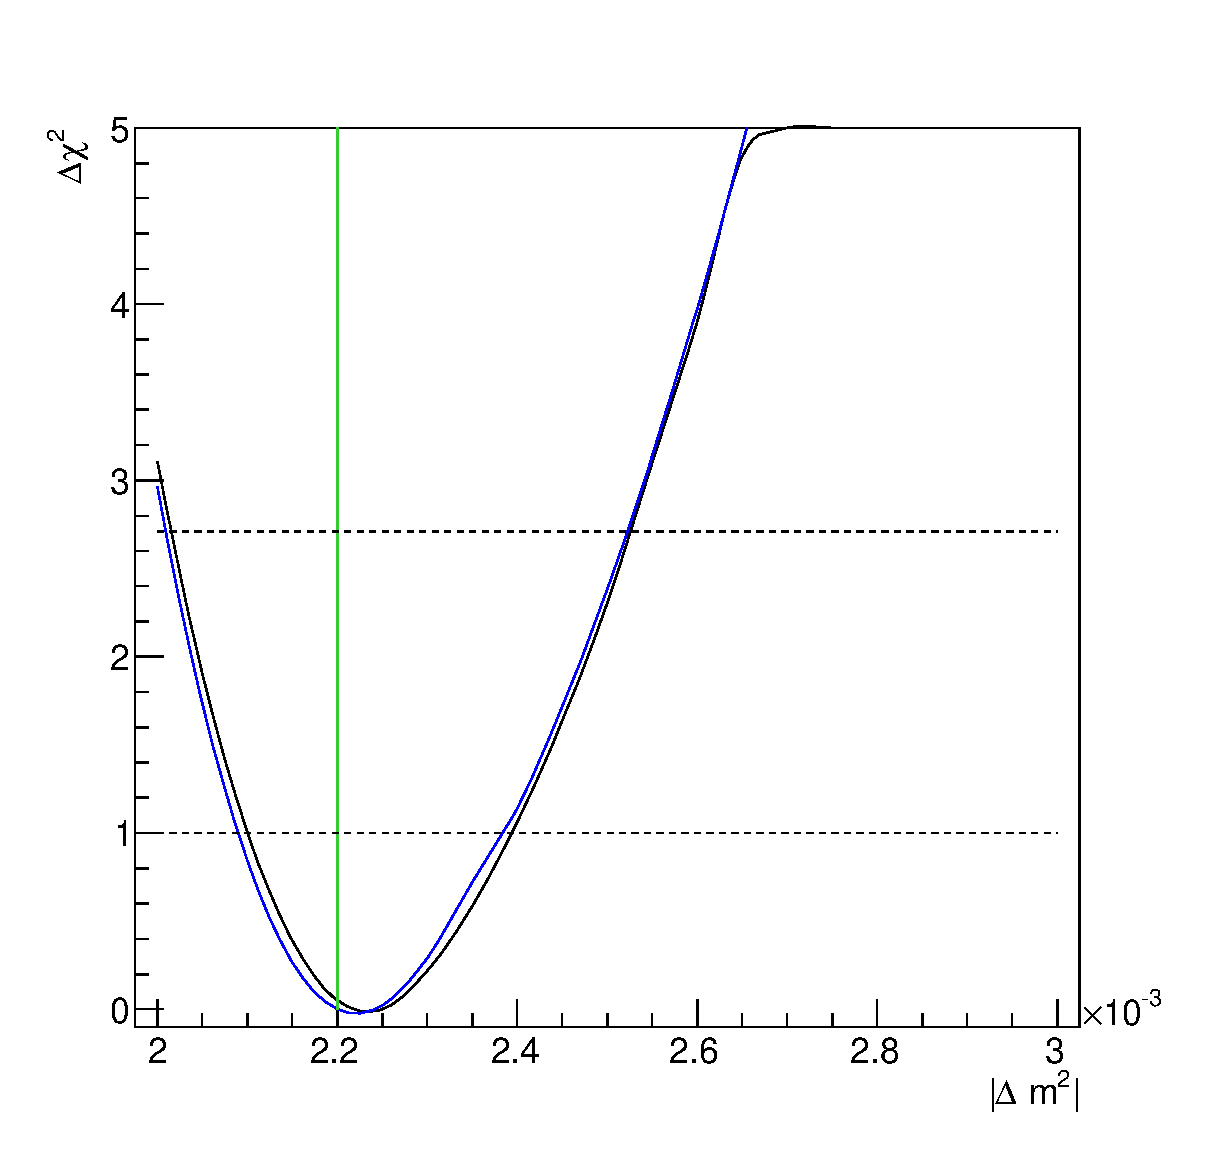
\includegraphics[width=9pc]{./images/appendix/fake_dataset_fits/realistic_fake_dataset5_chisq_dm23sq_global_min.eps}
\caption {
  $\Delta\chi^2$ as function of $|\Delta m^{2}|$ for fake dataset \#12.
  At each point, $\chi^2$ was minimized with respect to 
  $\sin^{2}\theta_{23}$, $\sin^{2}\theta_{13}$, $\delta_{CP}$
  and all relevant nuisance parameters for the joint analysis (black)
  and with respect to $\sin^{2}\theta_{23}$ and all relevant nuisance
  parameters for the disappearance analysis (blue).
}
\label{fig:toymc12_dchisq_Dmsq}
\end{minipage}
\hspace{0.02\linewidth}
\begin{minipage}[t]{0.22\linewidth}
\center
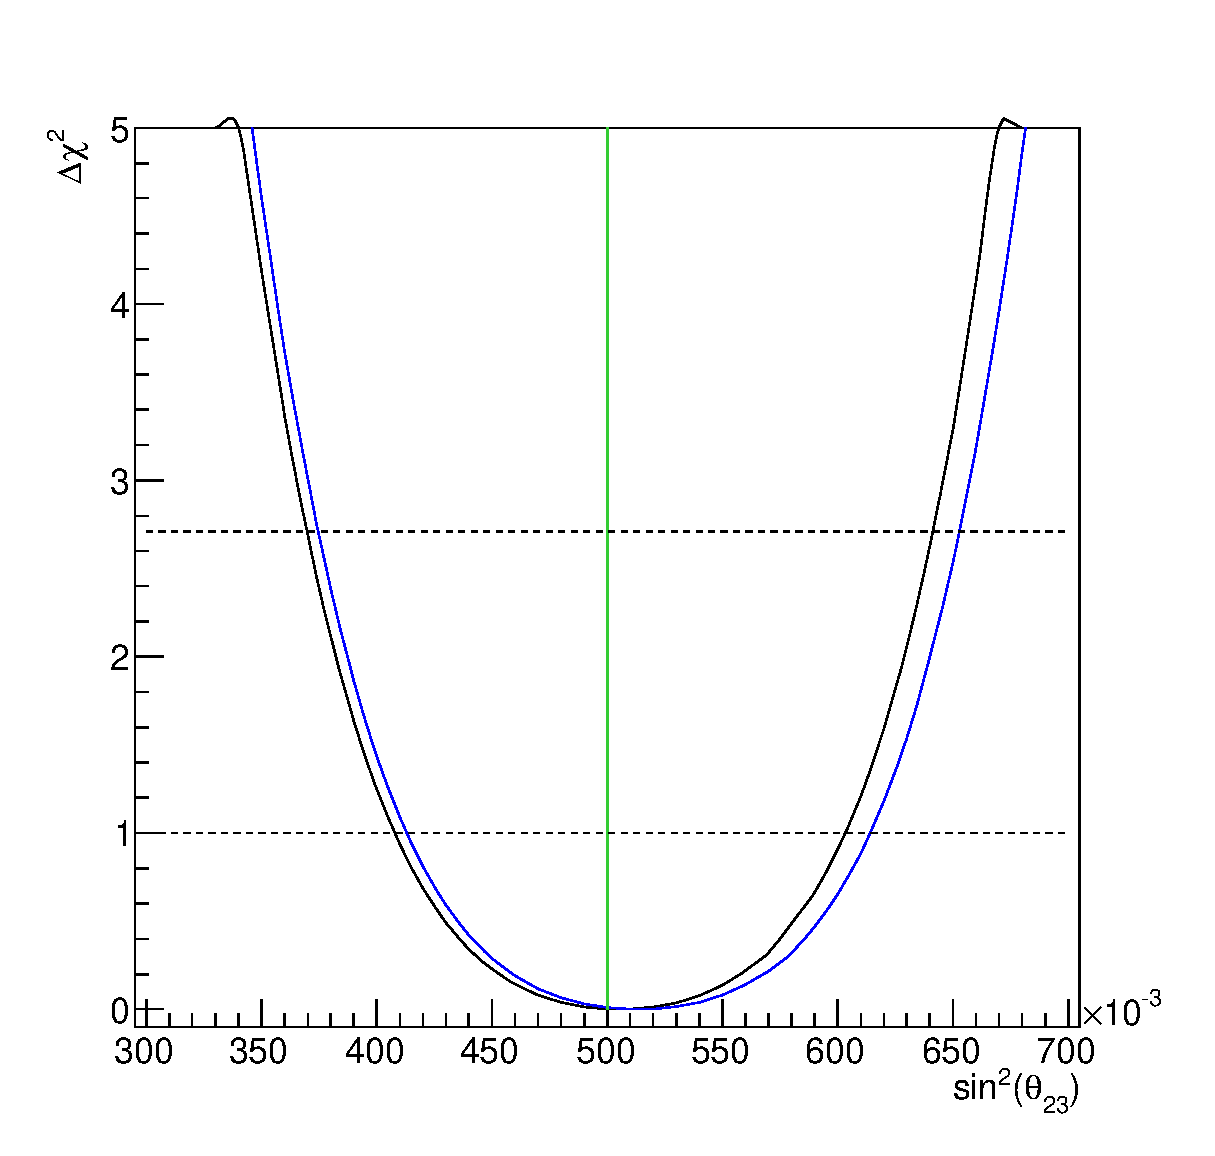
\includegraphics[width=9pc]{./images/appendix/fake_dataset_fits/realistic_fake_dataset5_chisq_theta23_global_min.eps}
\caption {
  $\Delta\chi^2$ as function of $sin^{2}\theta_{23}$ for fake dataset \#12.
  At each point, $\chi^2$ was minimized with respect to 
  $|\Delta m^{2}|$, $\sin^{2}\theta_{13}$, $\delta_{CP}$
  and all relevant nuisance parameters for the joint analysis (black)
  and with respect to $\sin^{2}\theta_{23}$ and all relevant nuisance
  parameters for the disappearance analysis (blue).
}
\label{fig:toymc12_dchisq_sinsqtheta23}
\end{minipage}
\hspace{0.02\linewidth}
\begin{minipage}[t]{0.22\linewidth}
\center
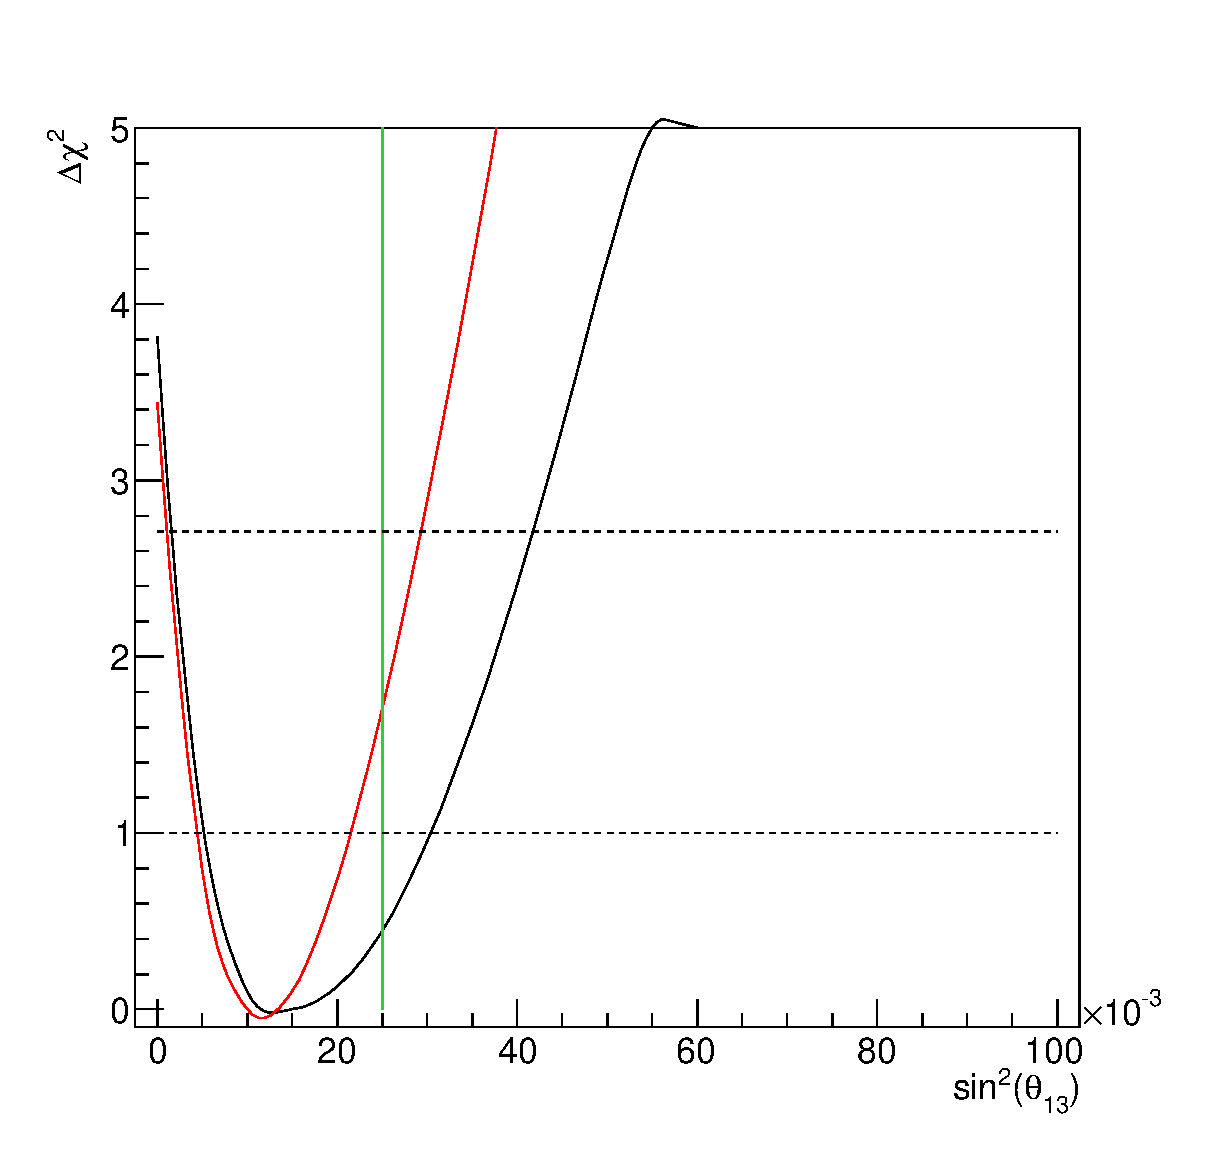
\includegraphics[width=9pc]{./images/appendix/fake_dataset_fits/realistic_fake_dataset5_chisq_theta13_global_min.eps}
\caption {
  $\Delta\chi^2$ as function of $sin^{2}\theta_{13}$ for fake dataset \#12.
  At each point, $\chi^2$ was minimized with respect to 
  $\sin^{2}\theta_{23}$, $\sin^{2}\theta_{13}$, $\delta_{CP}$
  and all relevant nuisance parameters for the joint analysis (black)
  and with respect to all relevant nuisance parameters 
  ($\delta_{CP}$ is fixed to 0) for the appearance analysis (red).
}
\label{fig:toymc12_dchisq_sinsqtheta13}
\end{minipage}
\hspace{0.02\linewidth}
\begin{minipage}[t]{0.22\linewidth}
\center
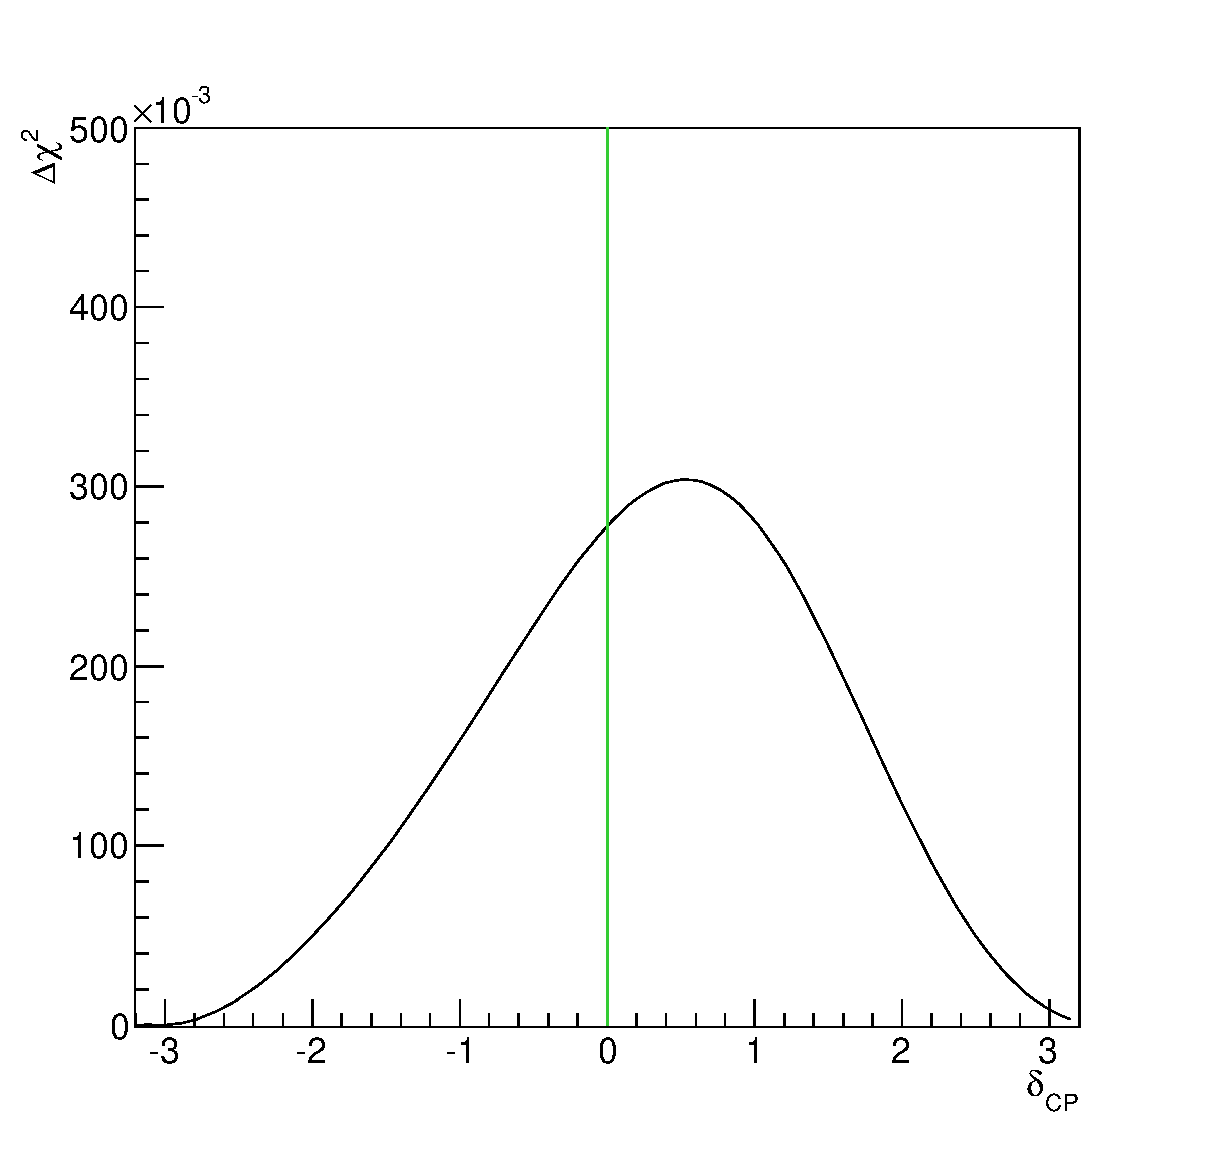
\includegraphics[width=9pc]{.//images/appendix/fake_dataset_fits/realistic_fake_dataset5_chisq_deltacp_global_min.eps}
\caption {
  $\Delta\chi^2$ as function of $\delta_{CP}$ for fake dataset \#12.
  At each point, $\chi^2$ was minimized with respect to 
  all oscillation parameters not shown (and not considered to be fixed)
  and all relevant nuisance parameters.
}
\label{fig:toymc12_dchisq_deltacp}
\end{minipage}
\vfill
\vspace*{0.7cm}
\begin{minipage}[t]{0.48\linewidth}
\center
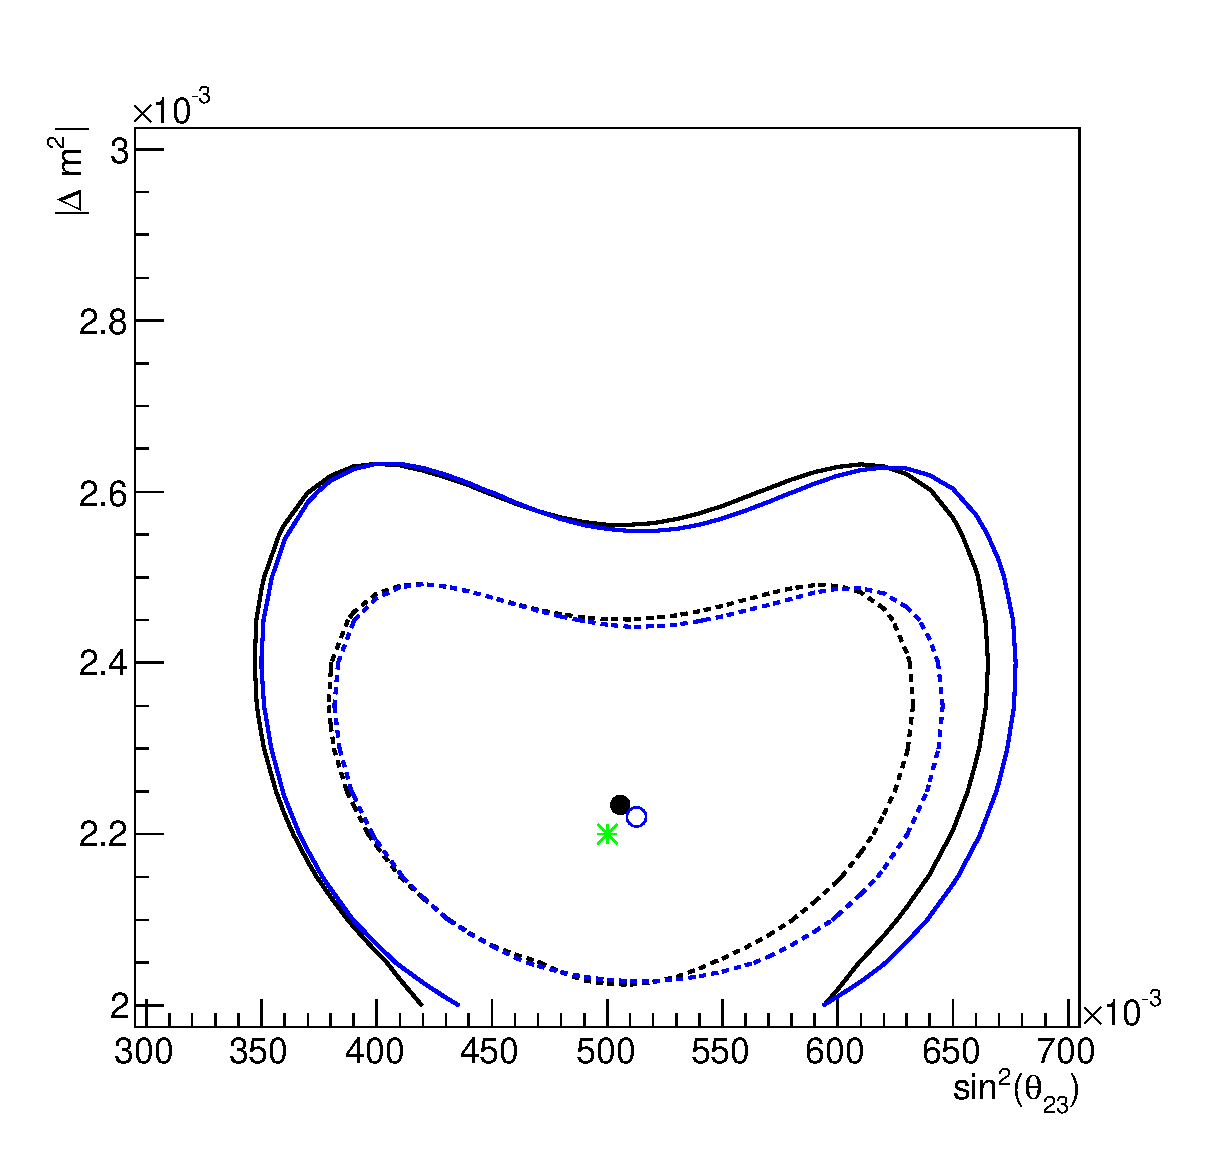
\includegraphics[width=15pc]{./images/appendix/fake_dataset_fits/realistic_fake_dataset5_chisq_theta23_dm23sq_global_min.eps}
\caption {
  68\% and 90\% CL regions in ($sin^{2}\theta_{23}$, $|\Delta m^{2}|$) space for fake dataset \#12.
  At each point, $\chi^2$ was minimized with respect to 
  $\sin^{2}\theta_{13}$, $\delta_{CP}$
  and all relevant nuisance parameters for the joint analysis (black)
  and with respect to all relevant nuisance parameters for the disappearance analysis (blue).
}
\label{fig:toymc12_confreg_sinsqtheta23_Dmsq}
\end{minipage}
\hspace{0.03\linewidth}
\begin{minipage}[t]{0.48\linewidth}
\center
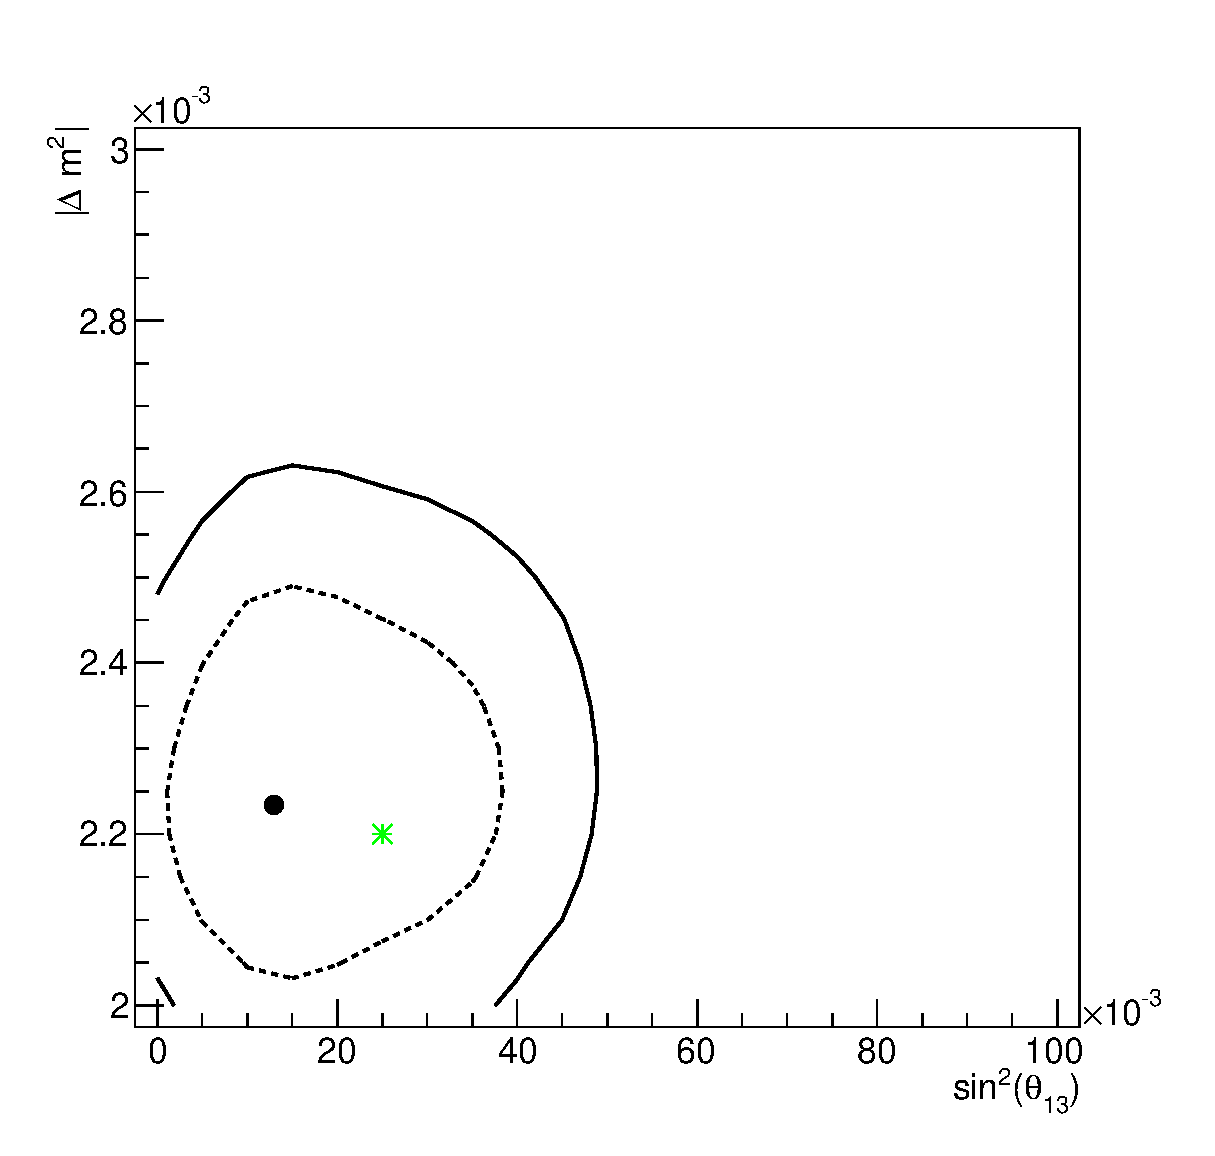
\includegraphics[width=15pc]{./images/appendix/fake_dataset_fits/realistic_fake_dataset5_chisq_theta13_dm23sq_global_min.eps}
\caption {
  68\% and 90\% CL regions in ($sin^{2}\theta_{13}$, $|\Delta m^{2}|$) space for fake dataset \#12.
  At each point, $\chi^2$ was minimized with respect to 
  all oscillation parameters not shown (and not considered to be fixed)
  and all relevant nuisance parameters.
}
\label{fig:toymc12_confreg_sinsqtheta13_Dmsq}
\end{minipage}

\vfill
\vspace*{0.7cm}

\begin{minipage}[t]{0.48\linewidth}
\center
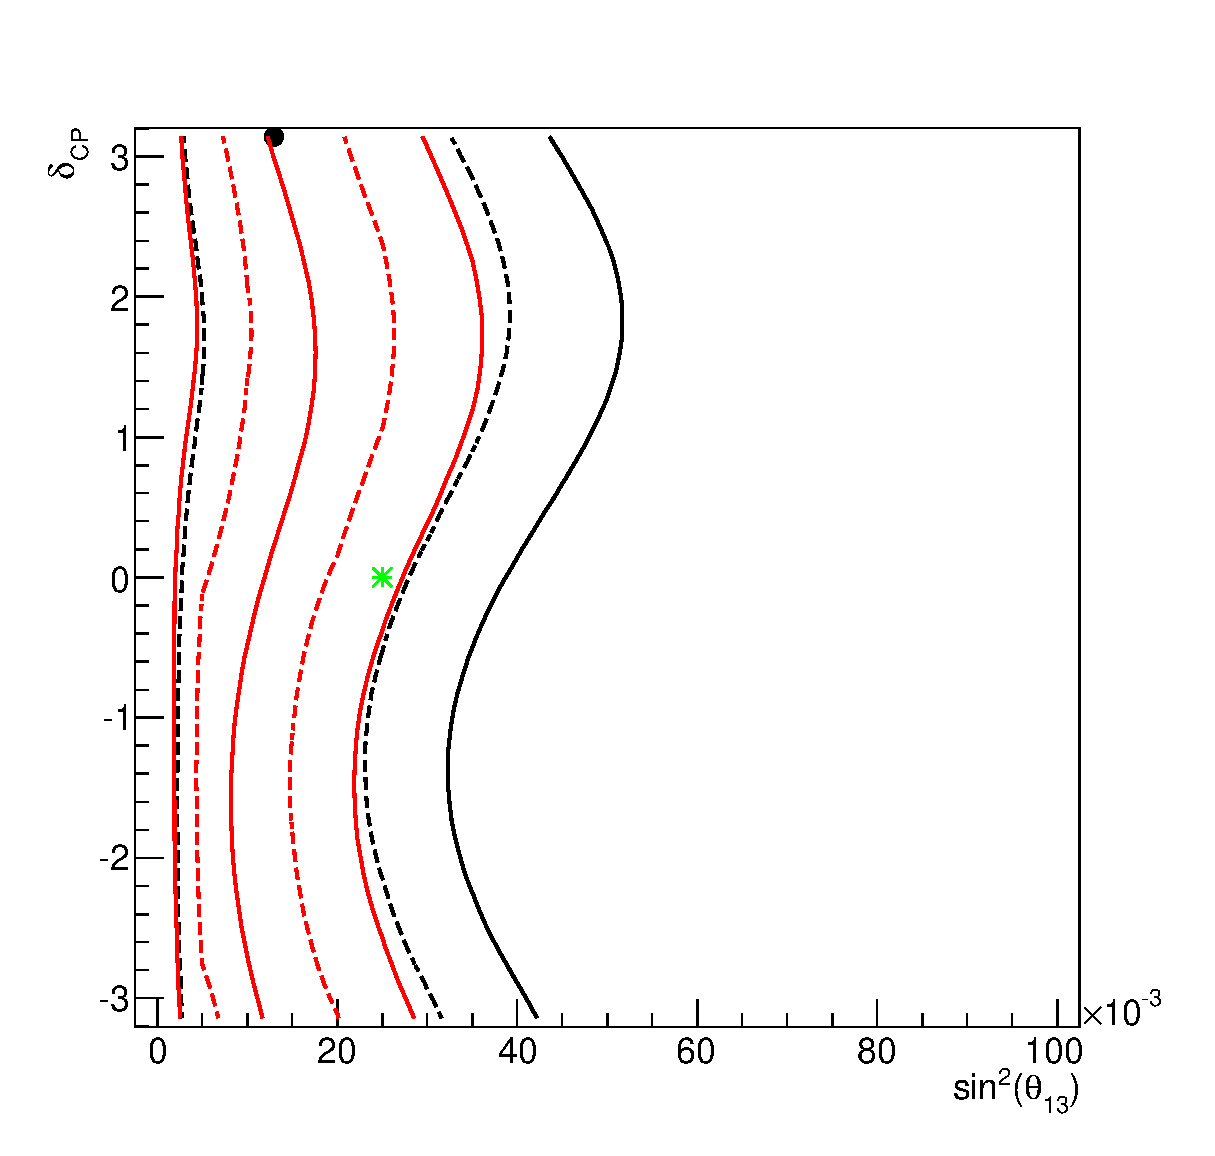
\includegraphics[width=15pc]{./images/appendix/fake_dataset_fits/realistic_fake_dataset5_chisq_theta13_deltacp_global_min.eps}
\caption {
  68\% and 90\% CL regions in ($sin^{2}\theta_{13}$, $\delta_{CP}$) space for fake dataset \#12.
  At each point, $\chi^2$ was minimized with respect to 
  $|\Delta m^{2}|$, $\sin^{2}\theta_{23}$
  and all relevant nuisance parameters for the joint analysis (black)
  and with respect to all relevant nuisance parameters for the appearance analysis (red).
  Notice that different methods are used to
  construct confidence regions for the joint analysis (global minimum) and for the 
  stand-alone appearance analysis (raster scan).
}
\label{fig:toymc12_confreg_sinsqtheta13_deltacp}
\end{minipage}
\hspace{0.03\linewidth}
\begin{minipage}[t]{0.48\linewidth}
\center
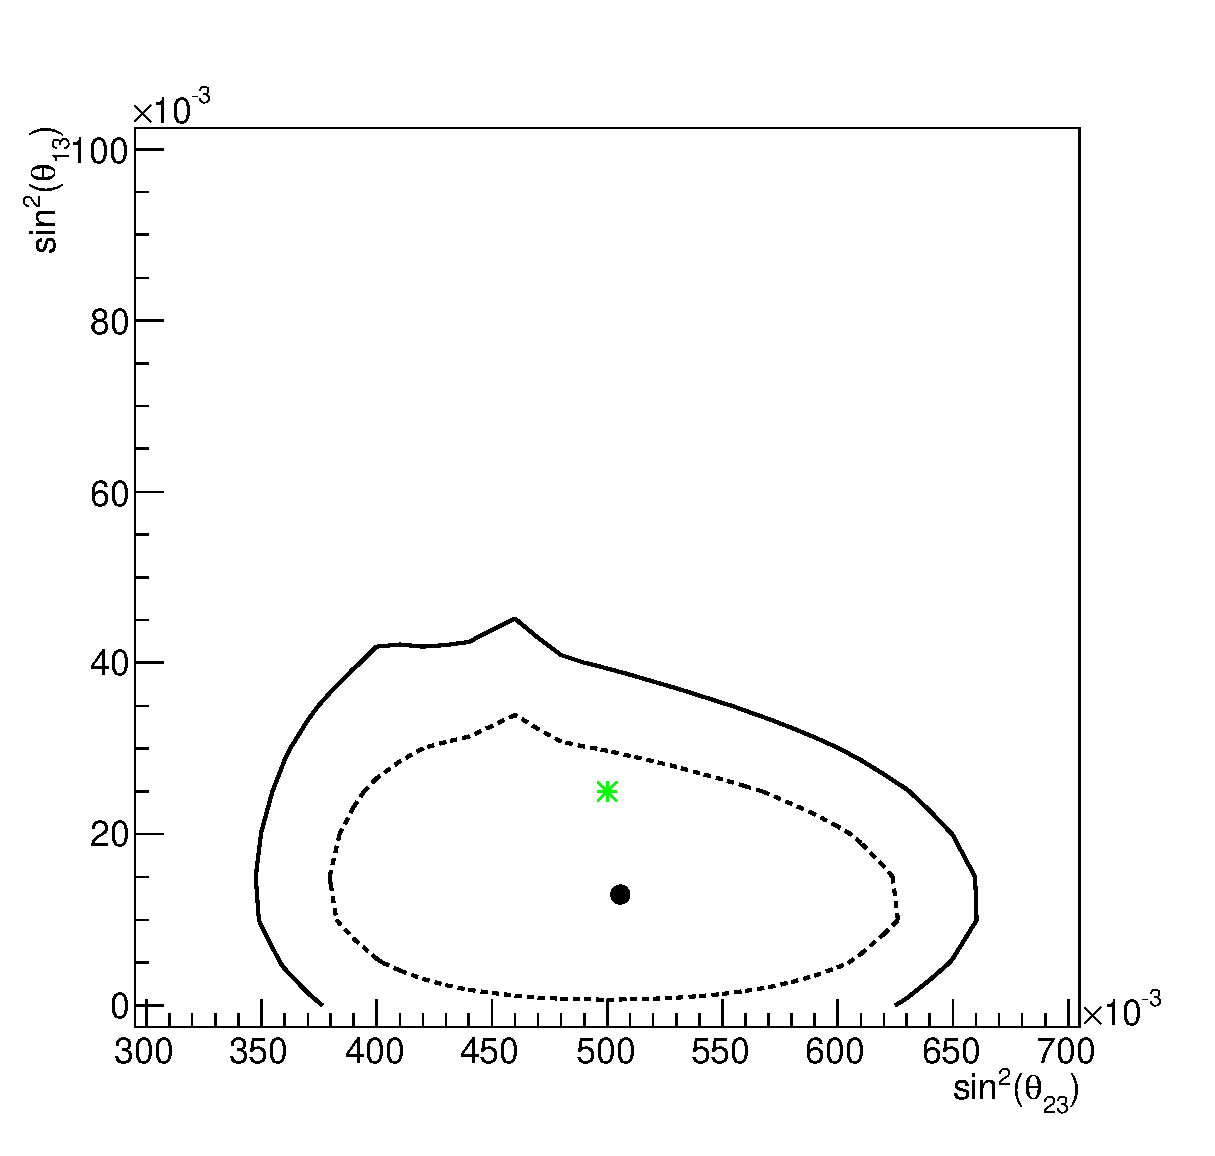
\includegraphics[width=15pc]{./images/appendix/fake_dataset_fits/realistic_fake_dataset5_chisq_theta13_theta23_global_min.eps}
\caption {
  68\% and 90\% CL regions in ($sin^{2}\theta_{23}$, $sin^{2}\theta_{13}$) space for fake dataset \#12.
  At each point, $\chi^2$ was minimized with respect to 
  all oscillation parameters not shown (and not considered to be fixed)
  and all relevant nuisance parameters.
}
\label{fig:toymc12_confreg_sinsqtheta23_sinsqtheta13}
\end{minipage}

\end{figure*}




% 
% 
% ..............................................
% Fake dataset #13
% 
%

\clearpage
\begin{figure*}[htb]

\begin{minipage}[t]{0.46\linewidth}
\center
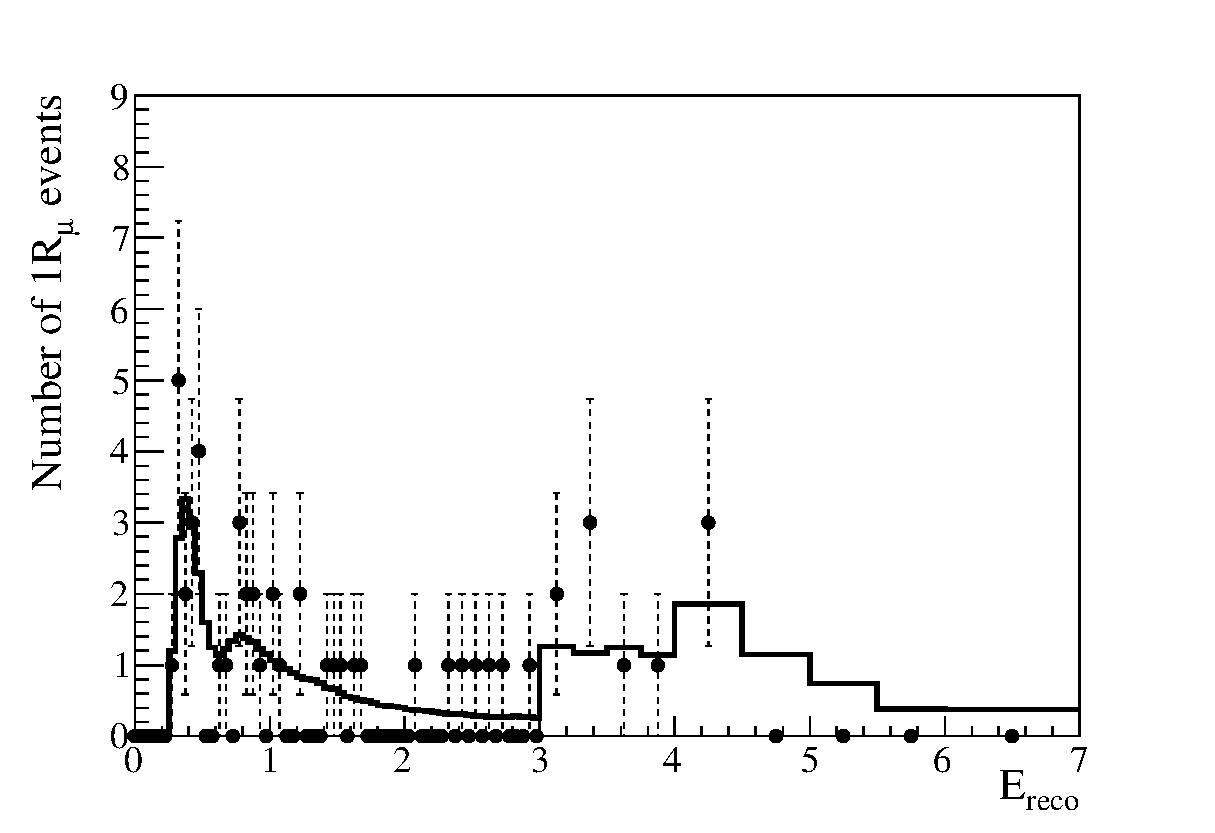
\includegraphics[width=15pc]{./images/appendix/fake_dataset_fits/realistic_fake_dataset6_ih_1st_1Rmu.eps}
\caption {
  Single $\mu$-like ring event best-fit reconstructed energy spectrum
  to fake dataset \#13.
}
\label{fig:toymc13_1Rmu_bestfit_spectrum}
\end{minipage}
\hspace{0.03\linewidth}
\begin{minipage}[t]{0.46\linewidth}
\center
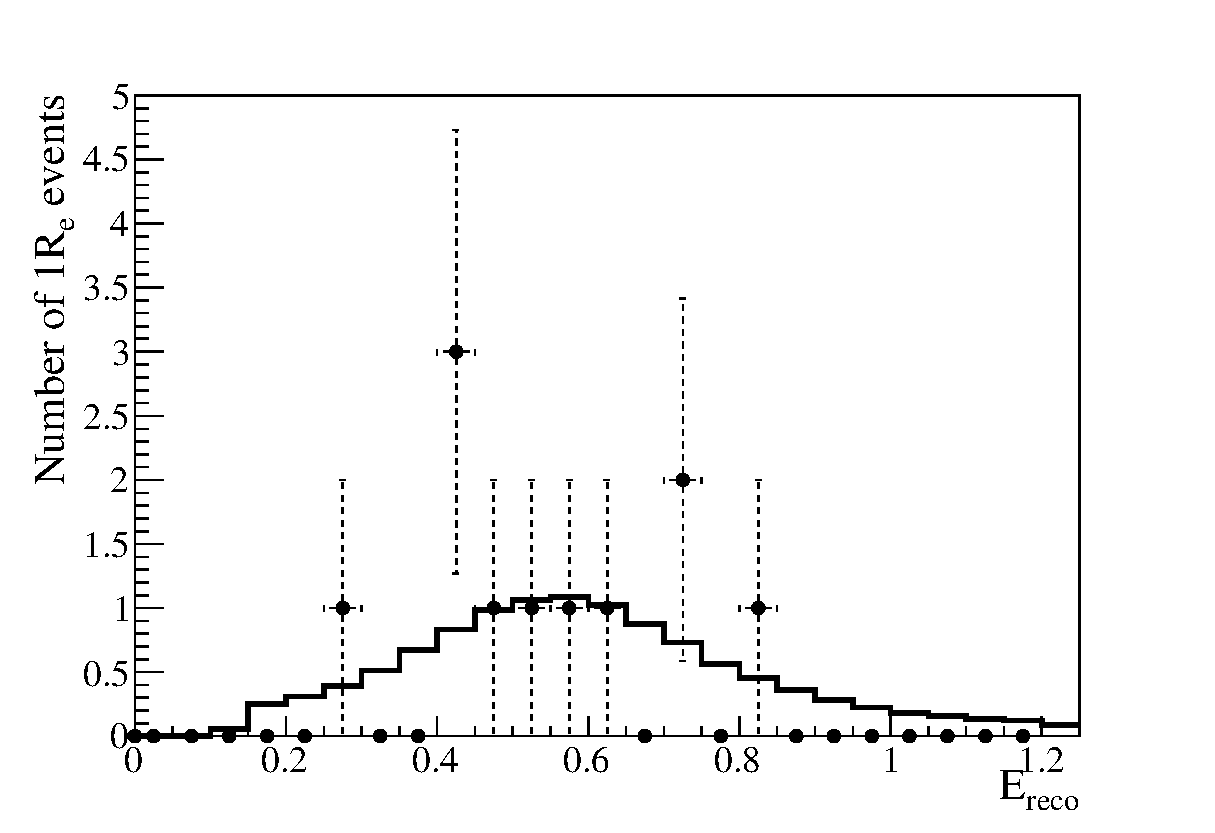
\includegraphics[width=15pc]{./images/appendix/fake_dataset_fits/realistic_fake_dataset6_ih_1st_1Re.eps}
\caption {
  Single e-like ring event best-fit reconstructed energy spectrum
  to fake dataset \#13.
}
\label{fig:toymc13_1Re_bestfit_spectrum}
\end{minipage}

\vfill
\vspace*{0.7cm}

\begin{minipage}[t]{0.90\linewidth}
\center
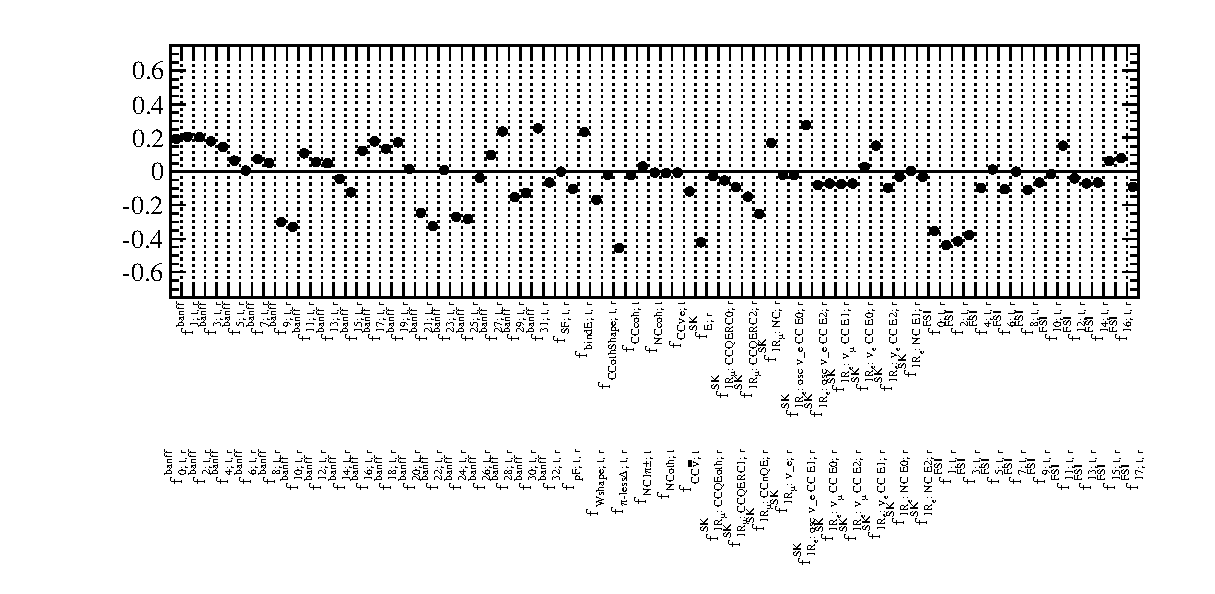
\includegraphics[width=30pc,angle=270]{./images/appendix/fake_dataset_fits/pulls_realistic_fake_dataset6_ih_1st.eps}
\caption {
  Systematic parameter pulls for the oscillation fit to fake dataset \#13.
}
\label{fig:toymc13_pulls}
\end{minipage}

\end{figure*}


%...........................................................
%
% chisq distributions used for calculating the fit p-values
%

\begin{figure*}[htb]

\begin{minipage}[t]{0.90\linewidth}
\center
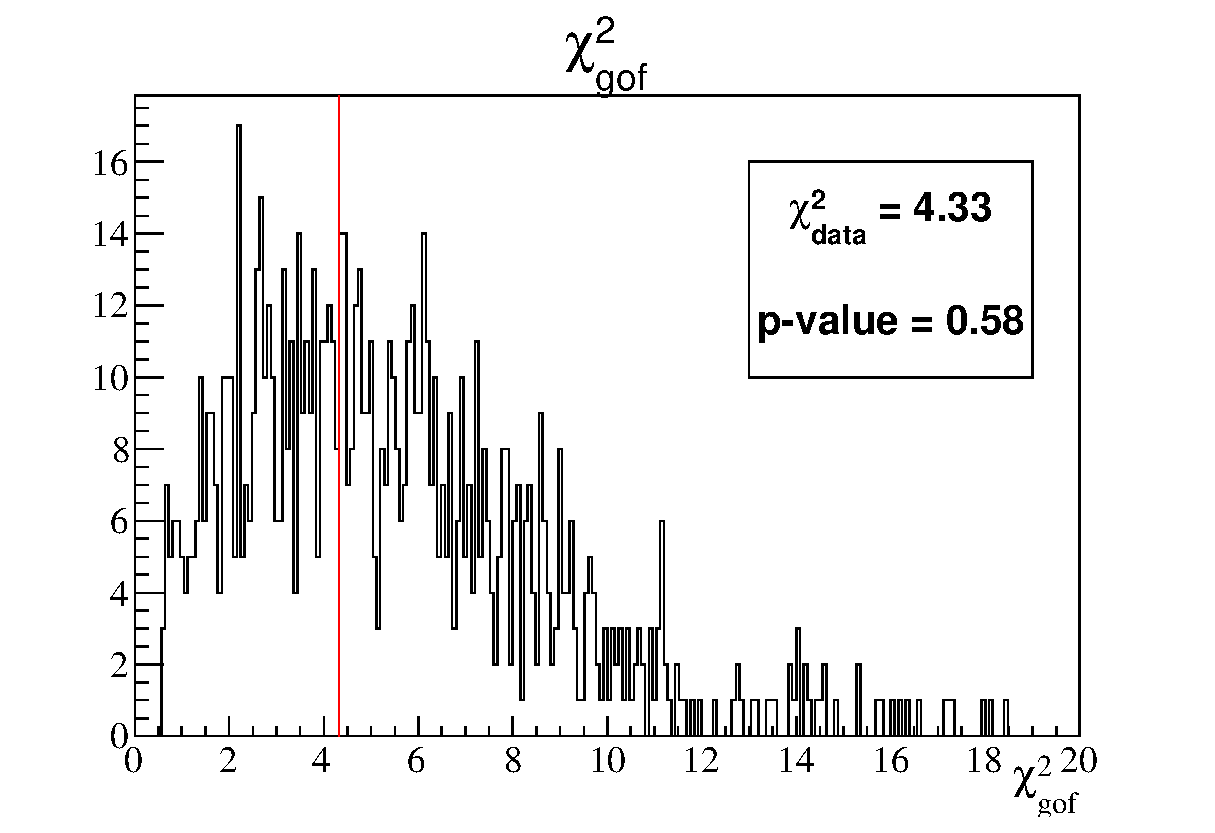
\includegraphics[width=30pc]{./images/appendix/fake_dataset_fits/realistic_fake_dataset6_ih_1st_gof_new.eps}
\caption {
  Distribution of $\chi^2_{gof}$, the goodness-of-fit (gof) $\chi^2$, 
  from 1k toy MC experiments generated at dataset \#13 joint 3-flavour analysis best-fit oscillation point.
  The $\chi^2_{gof}$ value for the dataset \#13 ($\chi^2_{data}$) is highlighted.
  All $\chi^2_{gof}$ values were computed 
  using the 5 (single $\mu$-like ring) + 3 (single e-like ring) 
  reconstructed energy binning scheme described in Sec.\ \ref{sec:goodness_of_fit}.
}
\label{fig:toymc13_gofchisq}
\end{minipage}

\vfill
\vspace*{0.7cm}

\begin{minipage}[t]{0.46\linewidth}
\center
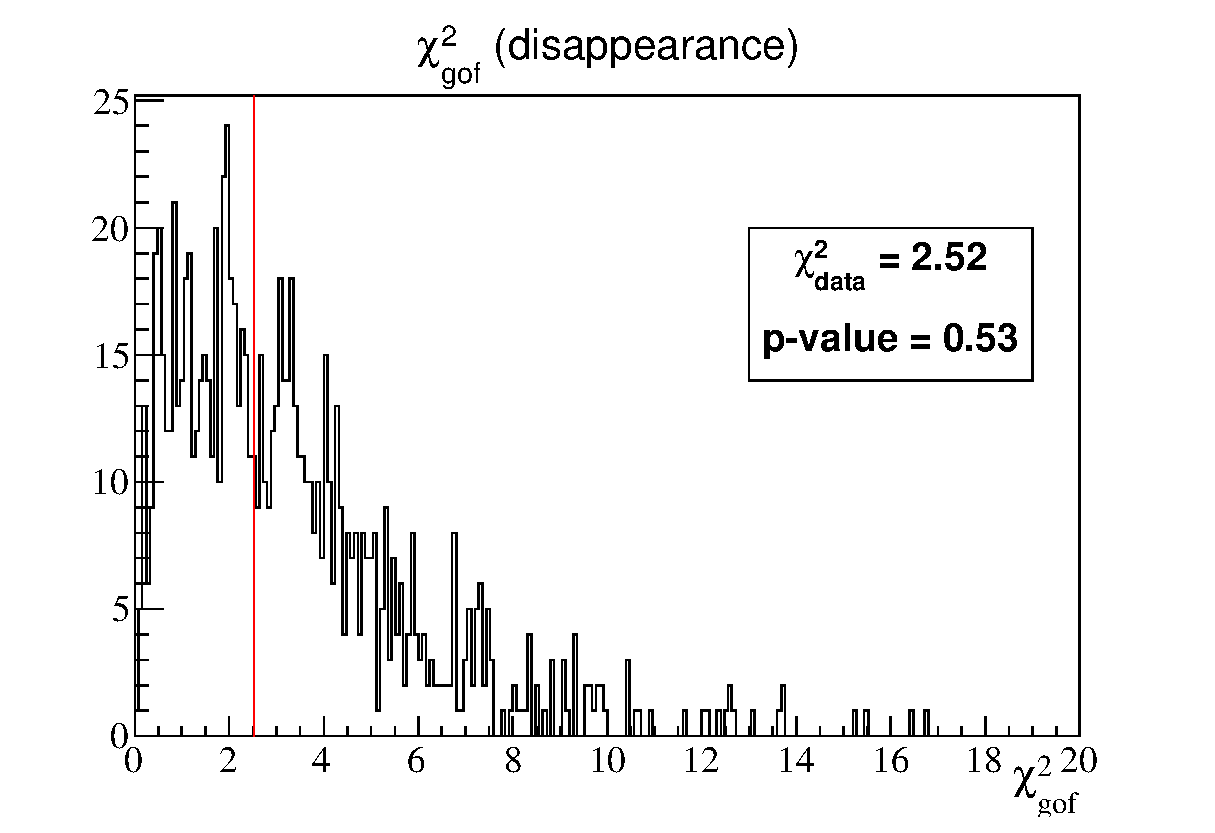
\includegraphics[width=18pc]{./images/appendix/fake_dataset_fits/realistic_fake_dataset6_ih_1st_gof_disap_new.eps}
\caption {
  Distribution of $\chi^2_{gof}$
  from 1k toy MC experiments generated at the dataset \#13 stand-alone 3-flavour $\nu_{\mu}$ disappearance analysis best-fit oscillation point.
  The $\chi^2_{gof}$ value for the dataset \#13 ($\chi^2_{data}$) is highlighted.
  All $\chi^2_{gof}$ values were computed 
  using the 5 (single $\mu$-like ring) 
  reconstructed energy binning scheme described in Sec.\ \ref{sec:goodness_of_fit}.
}
\label{fig:toymc13_gofchisq_disapp}
\end{minipage}
\hspace{0.03\linewidth}
\begin{minipage}[t]{0.46\linewidth}
\center
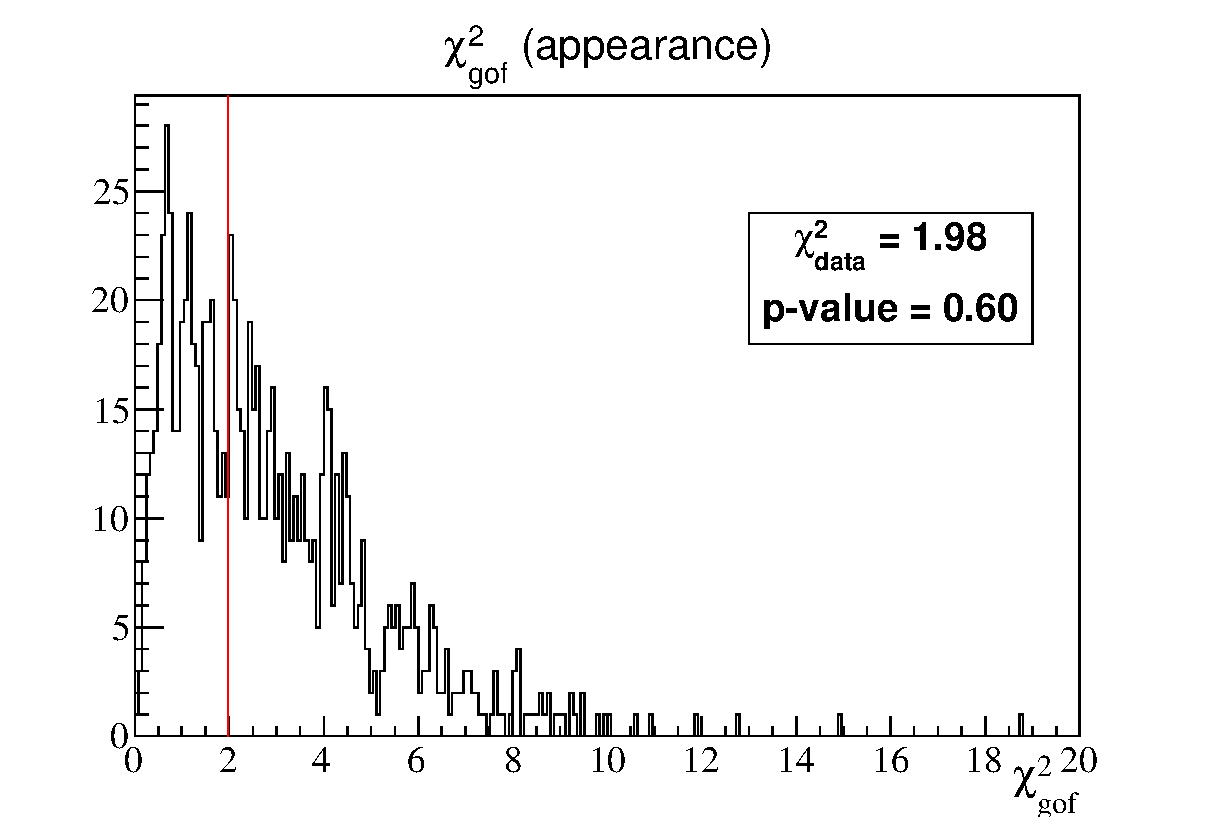
\includegraphics[width=18pc]{./images/appendix/fake_dataset_fits/realistic_fake_dataset6_ih_1st_gof_app_new.eps}
\caption {
  Distribution of $\chi^2_{gof}$
  from 1k toy MC experiments generated at the dataset \#13 stand-alone 3-flavour $\nu_{e}$ appearance analysis best-fit oscillation point.
  The $\chi^2_{gof}$ value for the dataset \#13 ($\chi^2_{data}$) is highlighted.
   All $\chi^2_{gof}$ values were computed 
  using the 3 (single e-like ring) 
  reconstructed energy binning scheme  as described in Sec.\ \ref{sec:goodness_of_fit}.
}
\label{fig:toymc13_gofchisq_app}
\end{minipage}

\end{figure*}




%
% delta\chisq and contours
%

\begin{figure*}[htb]

\begin{minipage}[t]{0.22\linewidth}
\center
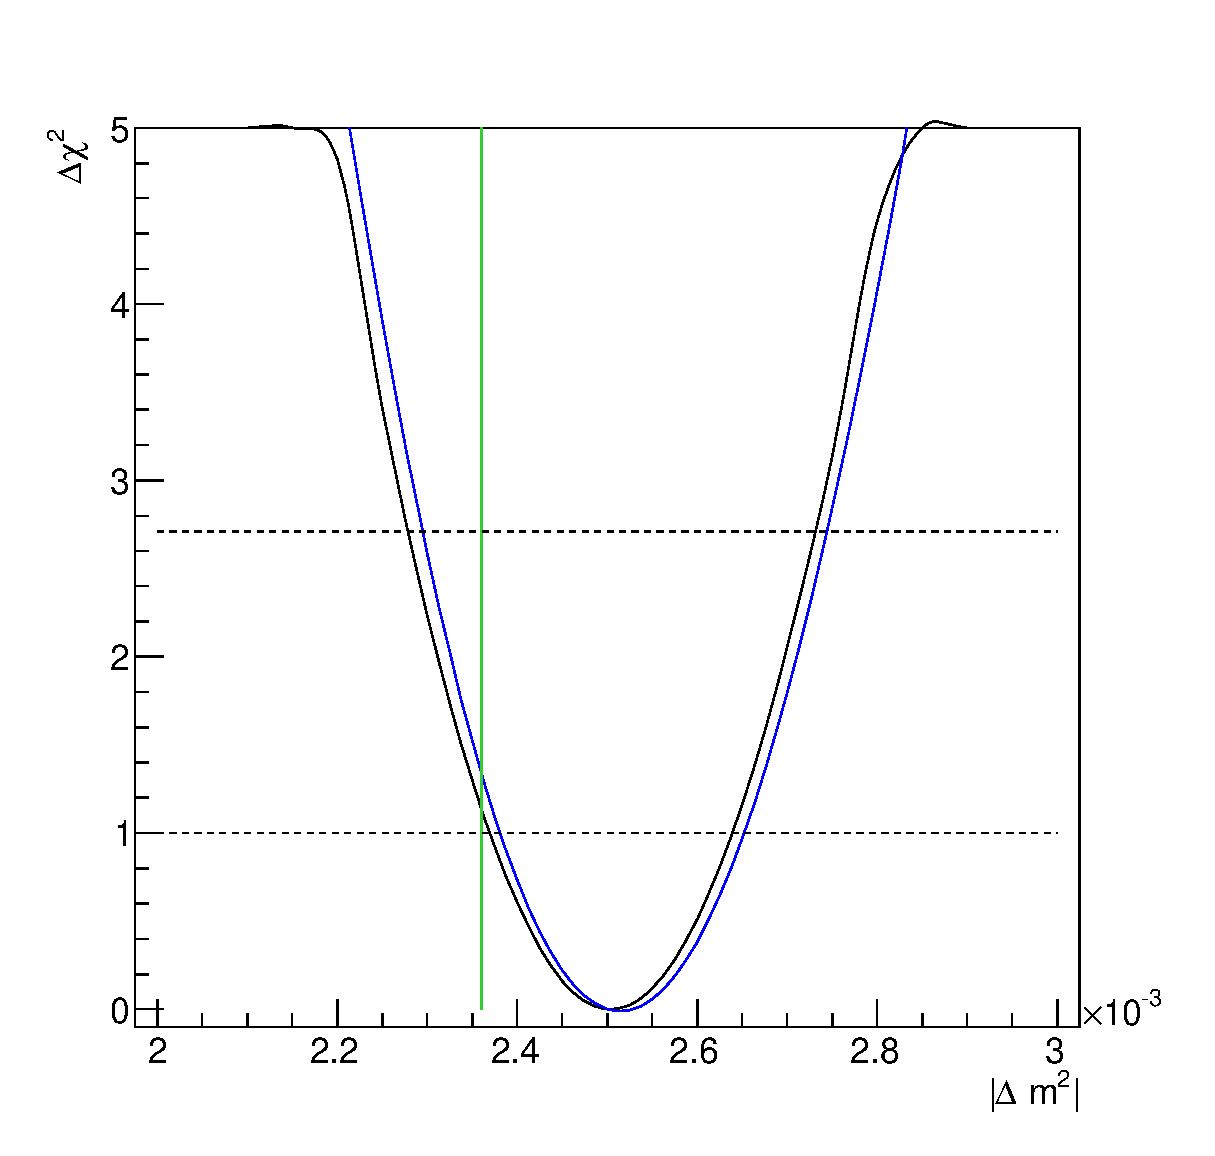
\includegraphics[width=9pc]{./images/appendix/fake_dataset_fits/realistic_fake_dataset6_chisq_dm23sq_global_min.eps}
\caption {
  $\Delta\chi^2$ as function of $|\Delta m^{2}|$ for fake dataset \#13.
  At each point, $\chi^2$ was minimized with respect to 
  $\sin^{2}\theta_{23}$, $\sin^{2}\theta_{13}$, $\delta_{CP}$
  and all relevant nuisance parameters for the joint analysis (black)
  and with respect to $\sin^{2}\theta_{23}$ and all relevant nuisance
  parameters for the disappearance analysis (blue).
}
\label{fig:toymc13_dchisq_Dmsq}
\end{minipage}
\hspace{0.02\linewidth}
\begin{minipage}[t]{0.22\linewidth}
\center
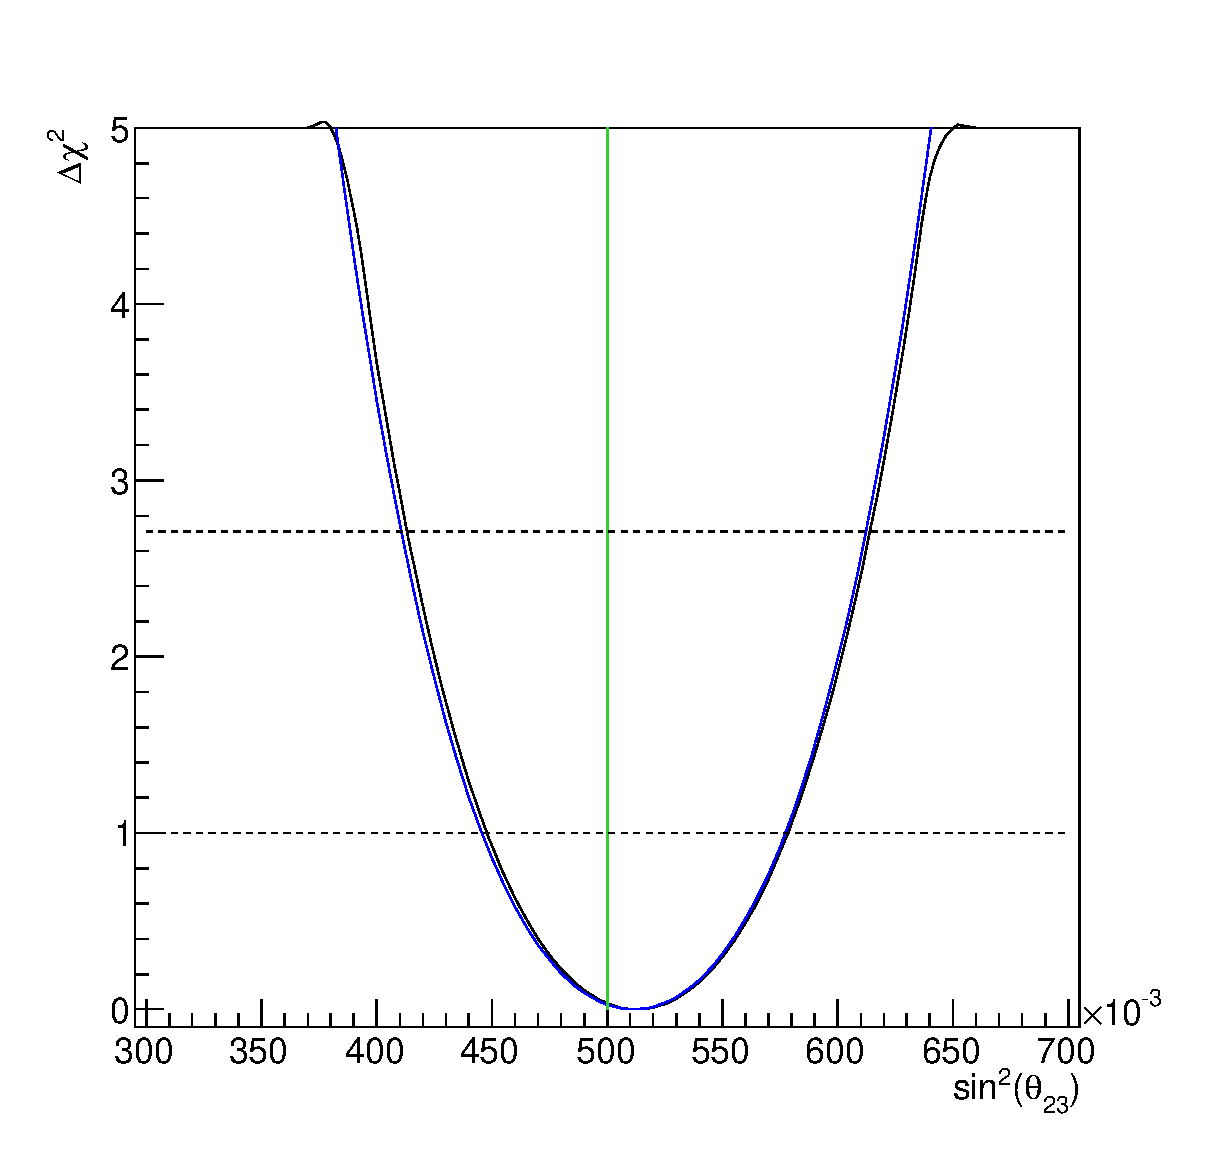
\includegraphics[width=9pc]{./images/appendix/fake_dataset_fits/realistic_fake_dataset6_chisq_theta23_global_min.eps}
\caption {
  $\Delta\chi^2$ as function of $sin^{2}\theta_{23}$ for fake dataset \#13.
  At each point, $\chi^2$ was minimized with respect to 
  $|\Delta m^{2}|$, $\sin^{2}\theta_{13}$, $\delta_{CP}$
  and all relevant nuisance parameters for the joint analysis (black)
  and with respect to $\sin^{2}\theta_{23}$ and all relevant nuisance
  parameters for the disappearance analysis (blue).
}
\label{fig:toymc13_dchisq_sinsqtheta23}
\end{minipage}
\hspace{0.02\linewidth}
\begin{minipage}[t]{0.22\linewidth}
\center
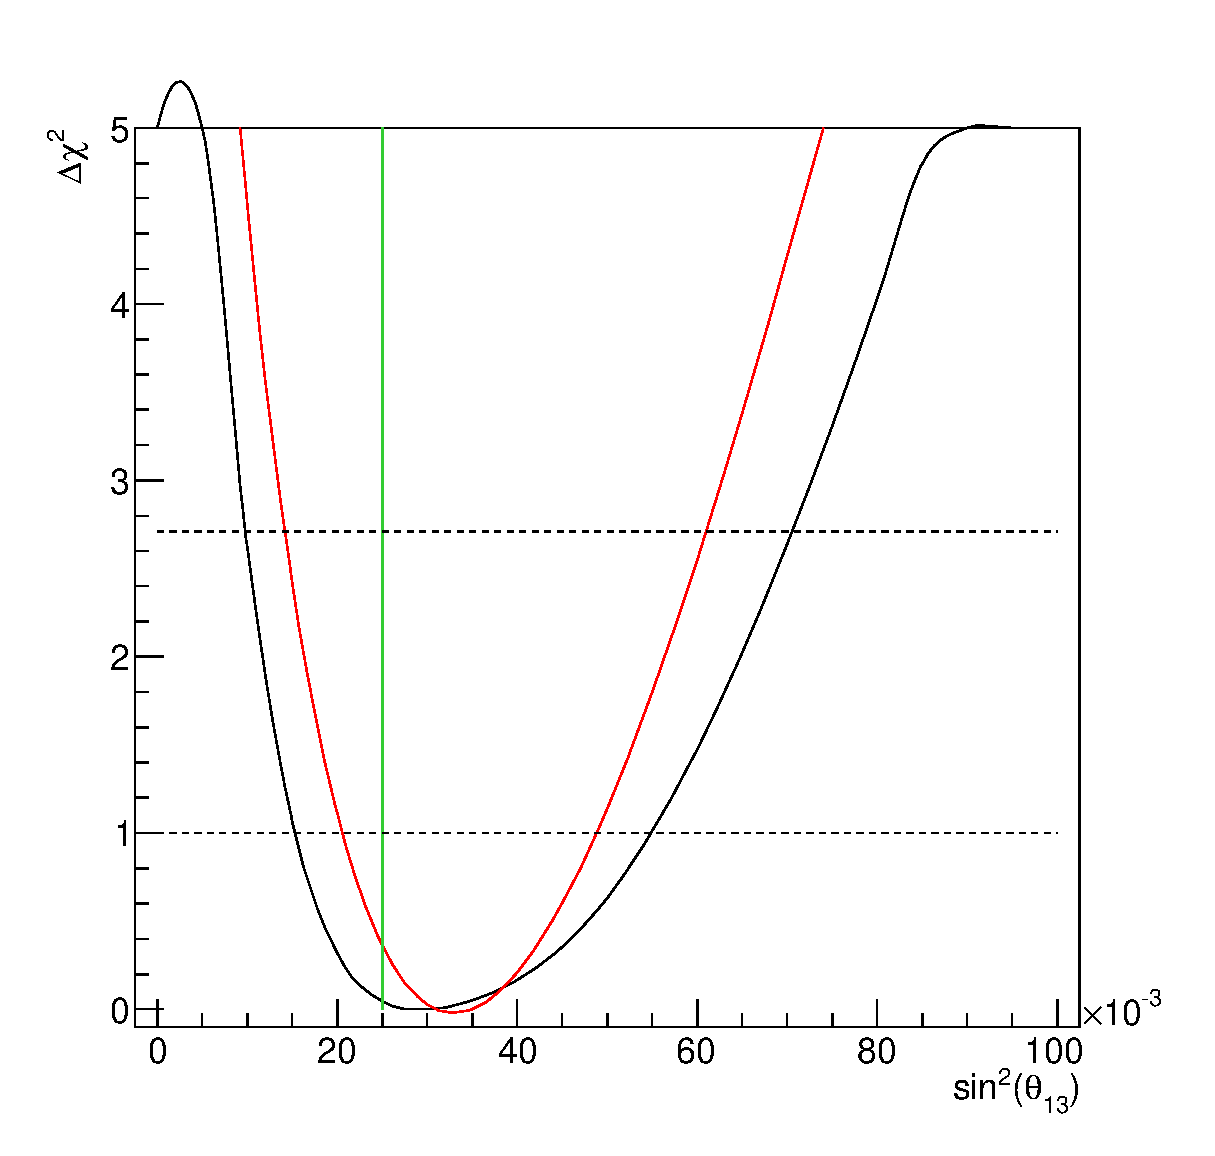
\includegraphics[width=9pc]{./images/appendix/fake_dataset_fits/realistic_fake_dataset6_chisq_theta13_global_min.eps}
\caption {
  $\Delta\chi^2$ as function of $sin^{2}\theta_{13}$ for fake dataset \#13.
  At each point, $\chi^2$ was minimized with respect to 
  $\sin^{2}\theta_{23}$, $\sin^{2}\theta_{13}$, $\delta_{CP}$
  and all relevant nuisance parameters for the joint analysis (black)
  and with respect to all relevant nuisance parameters 
  ($\delta_{CP}$ is fixed to 0) for the appearance analysis (red).
}
\label{fig:toymc13_dchisq_sinsqtheta13}
\end{minipage}
\hspace{0.02\linewidth}
\begin{minipage}[t]{0.22\linewidth}
\center
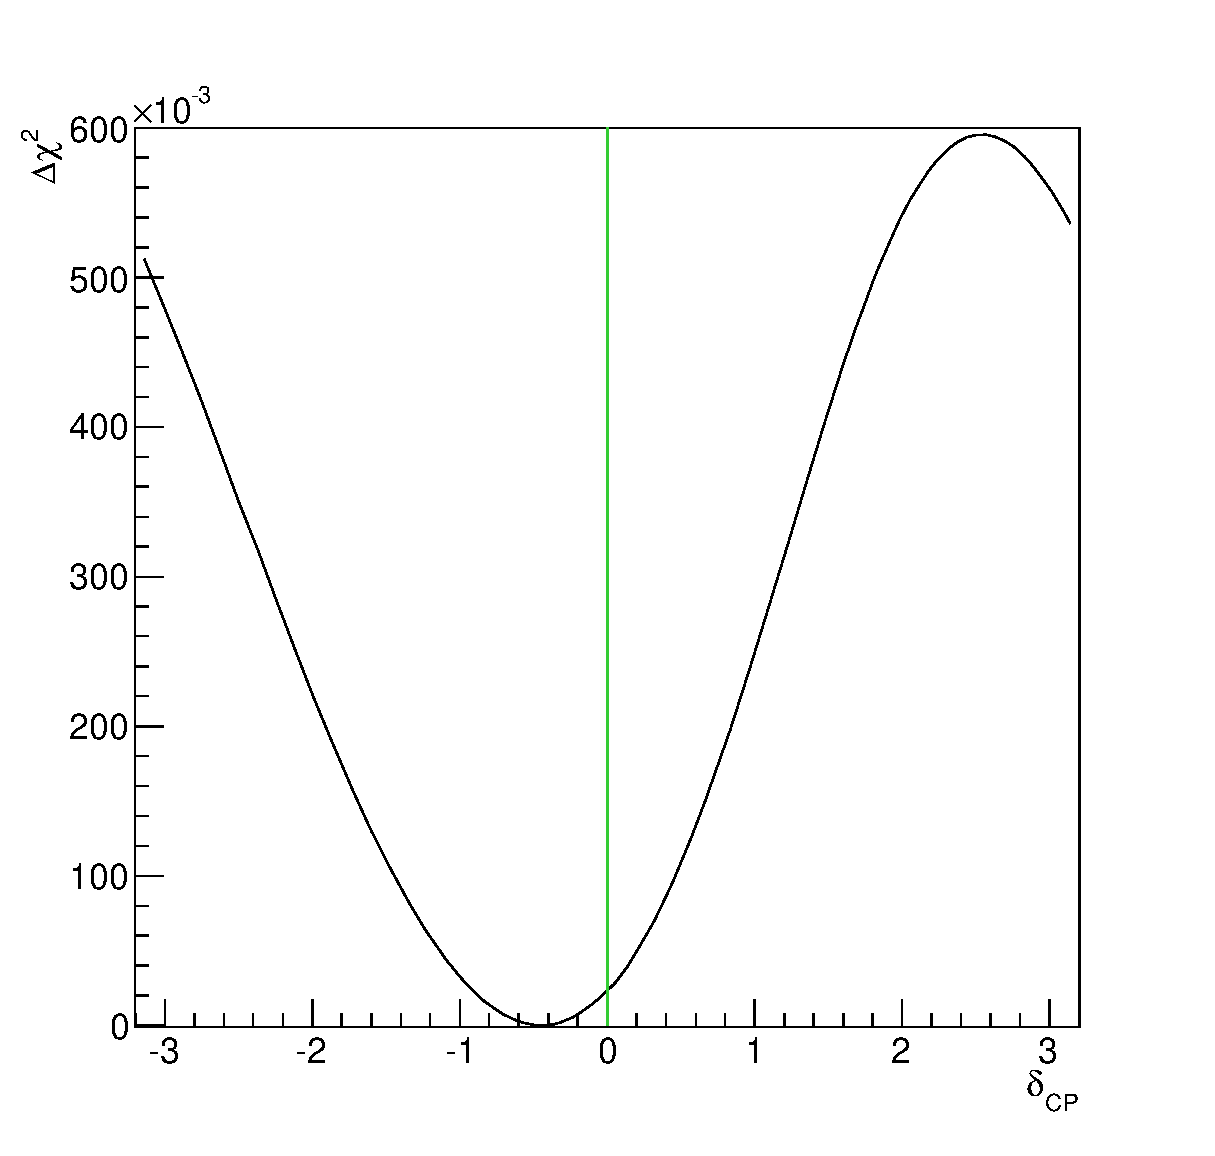
\includegraphics[width=9pc]{.//images/appendix/fake_dataset_fits/realistic_fake_dataset6_chisq_deltacp_global_min.eps}
\caption {
  $\Delta\chi^2$ as function of $\delta_{CP}$ for fake dataset \#13.
  At each point, $\chi^2$ was minimized with respect to 
  all oscillation parameters not shown (and not considered to be fixed)
  and all relevant nuisance parameters.
}
\label{fig:toymc13_dchisq_deltacp}
\end{minipage}
\vfill
\vspace*{0.7cm}
\begin{minipage}[t]{0.48\linewidth}
\center
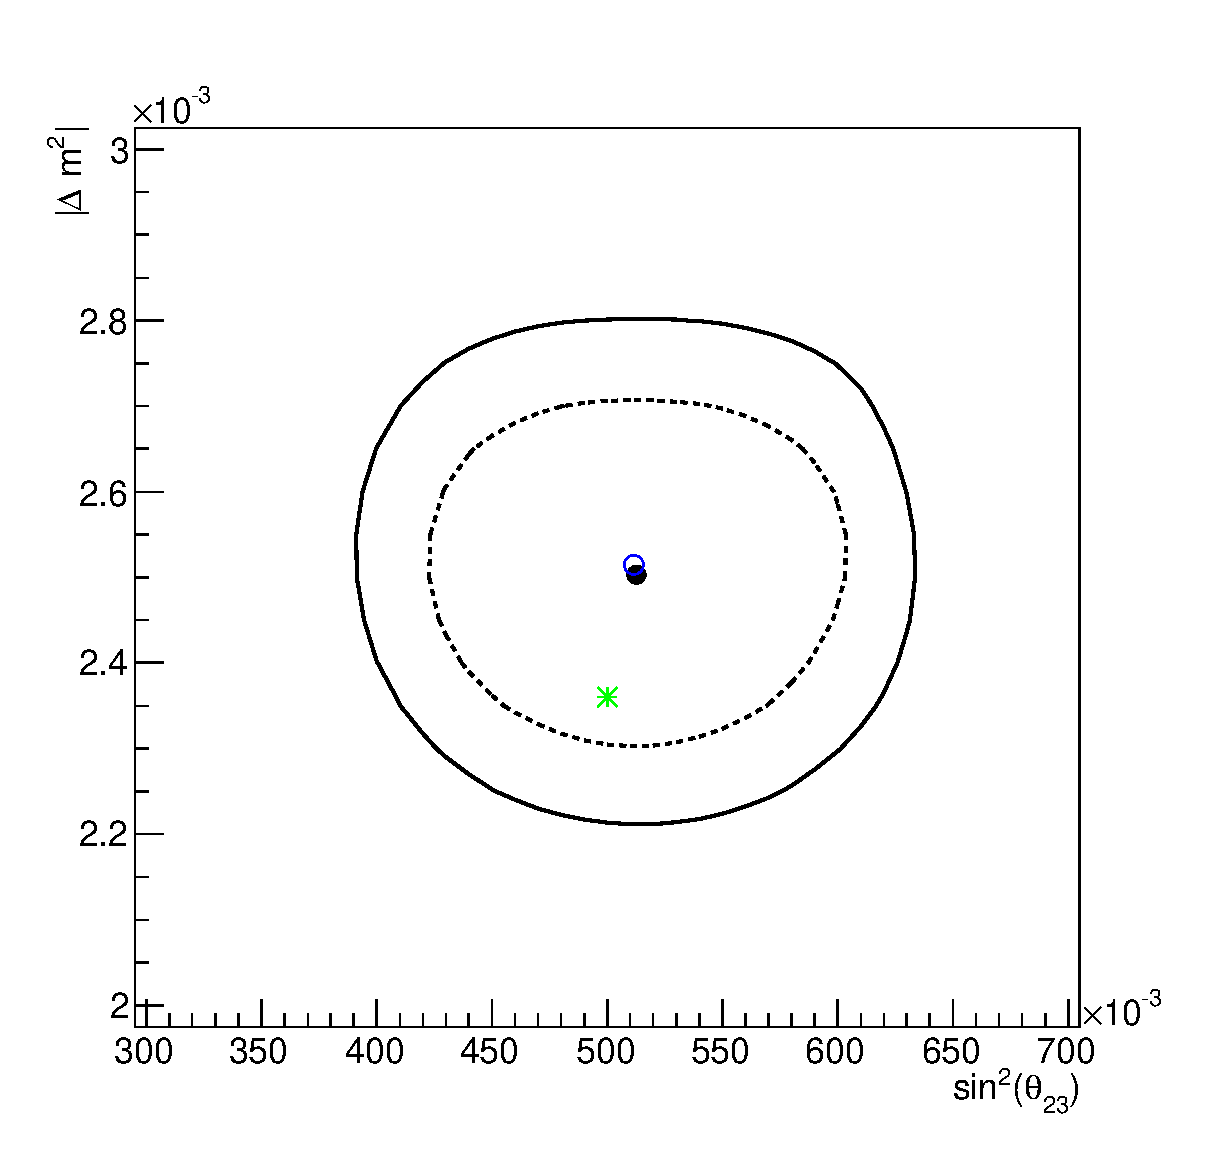
\includegraphics[width=15pc]{./images/appendix/fake_dataset_fits/realistic_fake_dataset6_chisq_theta23_dm23sq_global_min.eps}
\caption {
  68\% and 90\% CL regions in ($sin^{2}\theta_{23}$, $|\Delta m^{2}|$) space for fake dataset \#13.
  At each point, $\chi^2$ was minimized with respect to 
  $\sin^{2}\theta_{13}$, $\delta_{CP}$
  and all relevant nuisance parameters for the joint analysis (black)
  and with respect to all relevant nuisance parameters for the disappearance analysis (blue).
}
\label{fig:toymc13_confreg_sinsqtheta23_Dmsq}
\end{minipage}
\hspace{0.03\linewidth}
\begin{minipage}[t]{0.48\linewidth}
\center
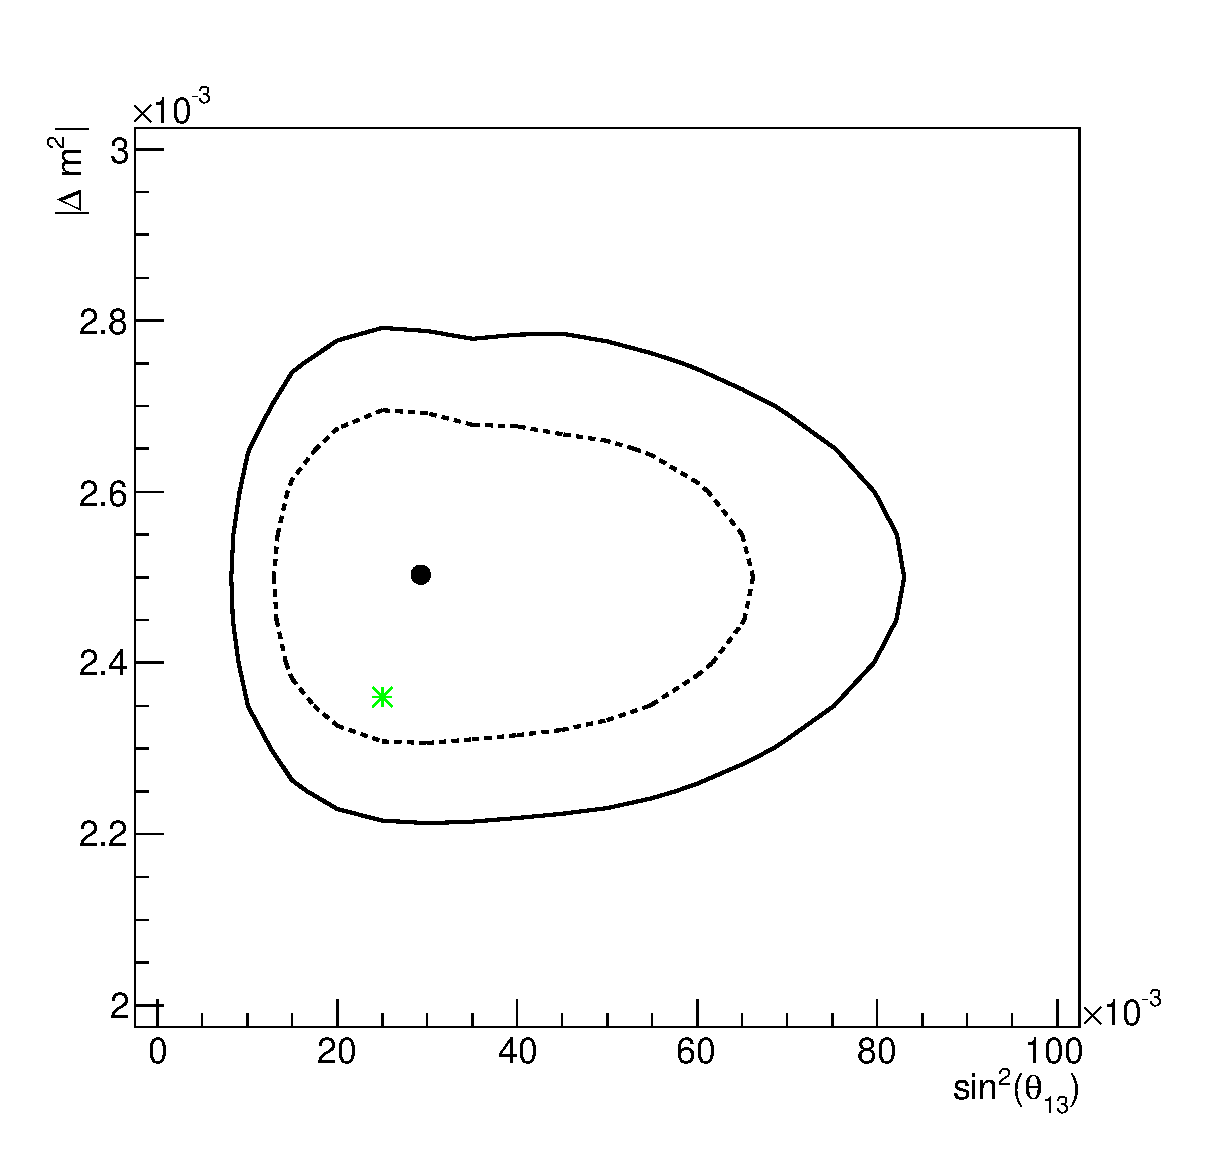
\includegraphics[width=15pc]{./images/appendix/fake_dataset_fits/realistic_fake_dataset6_chisq_theta13_dm23sq_global_min.eps}
\caption {
  68\% and 90\% CL regions in ($sin^{2}\theta_{13}$, $|\Delta m^{2}|$) space for fake dataset \#13.
  At each point, $\chi^2$ was minimized with respect to 
  all oscillation parameters not shown (and not considered to be fixed)
  and all relevant nuisance parameters.
}
\label{fig:toymc13_confreg_sinsqtheta13_Dmsq}
\end{minipage}

\vfill
\vspace*{0.7cm}

\begin{minipage}[t]{0.48\linewidth}
\center
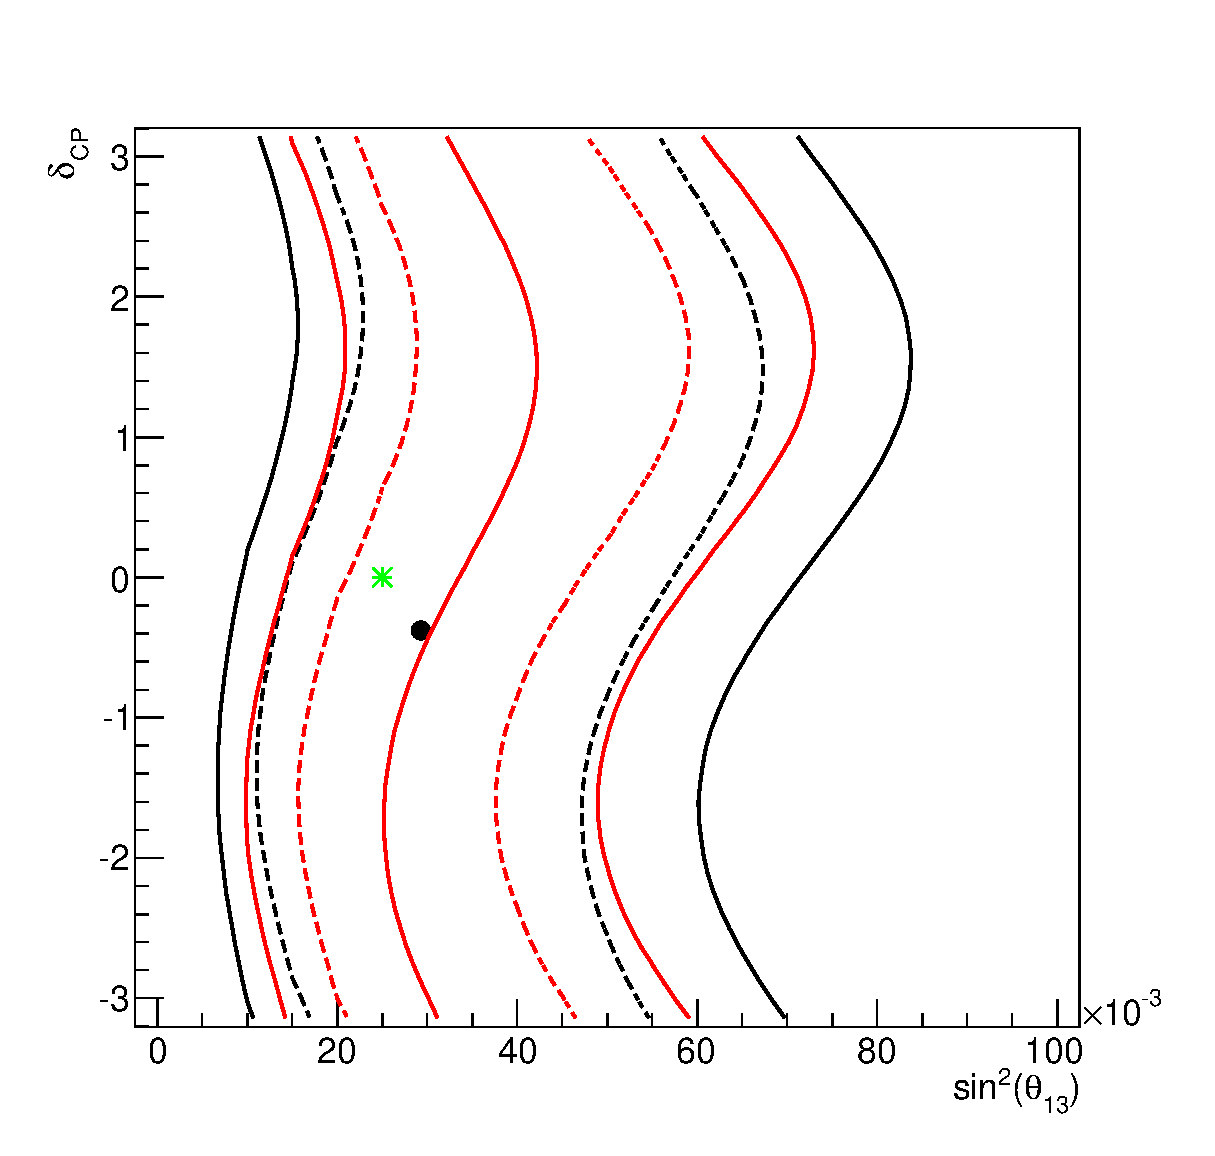
\includegraphics[width=15pc]{./images/appendix/fake_dataset_fits/realistic_fake_dataset6_chisq_theta13_deltacp_global_min.eps}
\caption {
  68\% and 90\% CL regions in ($sin^{2}\theta_{13}$, $\delta_{CP}$) space for fake dataset \#13.
  At each point, $\chi^2$ was minimized with respect to 
  $|\Delta m^{2}|$, $\sin^{2}\theta_{23}$
  and all relevant nuisance parameters for the joint analysis (black)
  and with respect to all relevant nuisance parameters for the appearance analysis (red).
  Notice that different methods are used to
  construct confidence regions for the joint analysis (global minimum) and for the 
  stand-alone appearance analysis (raster scan).
}
\label{fig:toymc13_confreg_sinsqtheta13_deltacp}
\end{minipage}
\hspace{0.03\linewidth}
\begin{minipage}[t]{0.48\linewidth}
\center
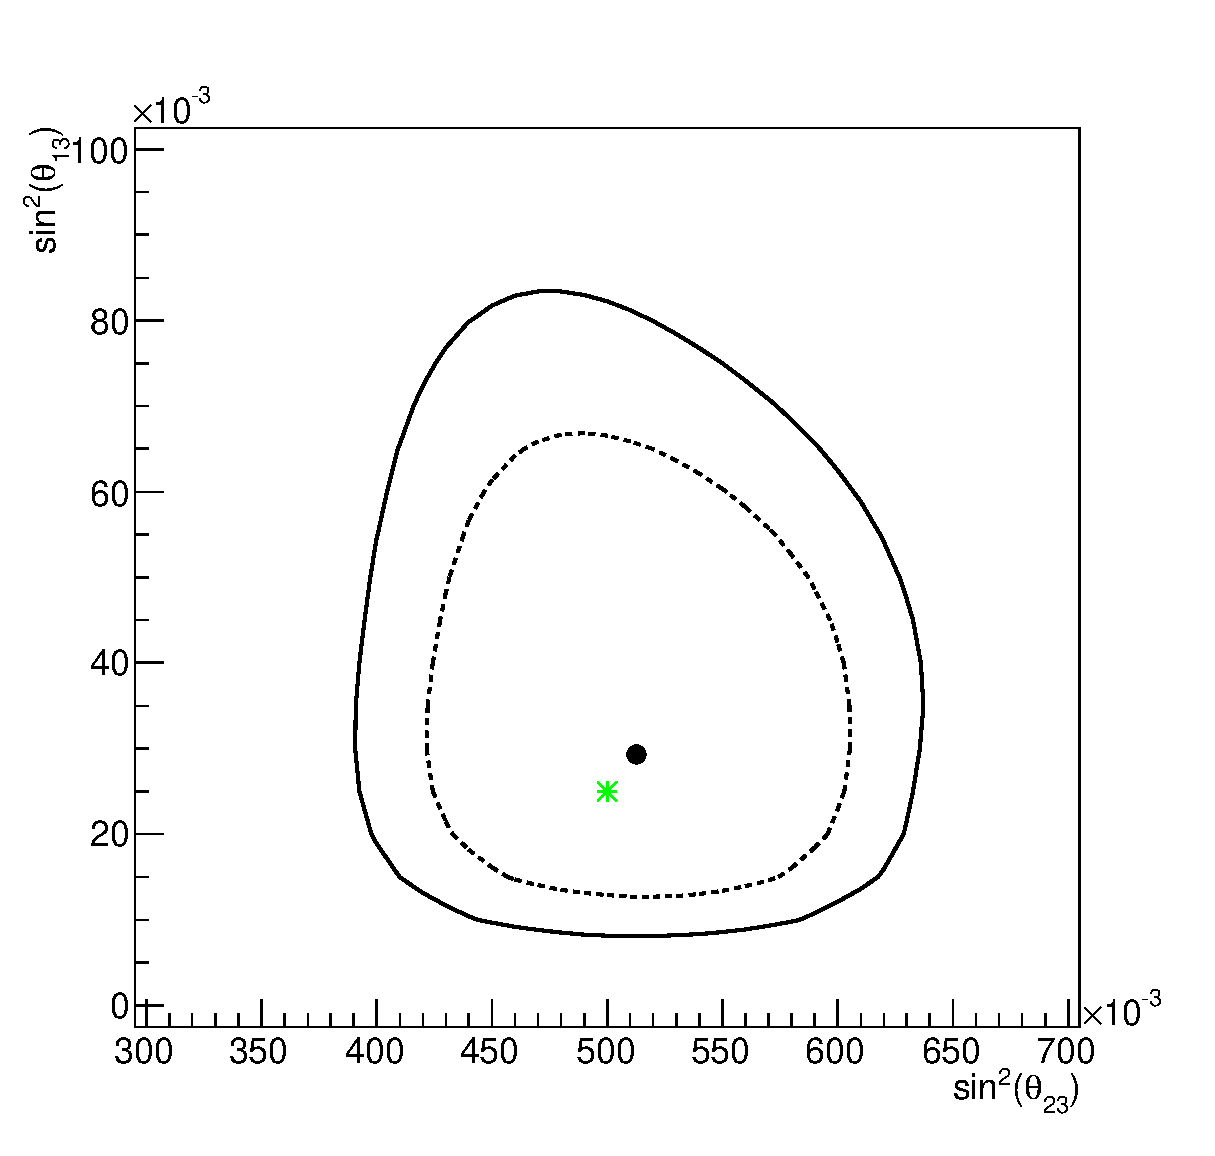
\includegraphics[width=15pc]{./images/appendix/fake_dataset_fits/realistic_fake_dataset6_chisq_theta13_theta23_global_min.eps}
\caption {
  68\% and 90\% CL regions in ($sin^{2}\theta_{23}$, $sin^{2}\theta_{13}$) space for fake dataset \#13.
  At each point, $\chi^2$ was minimized with respect to 
  all oscillation parameters not shown (and not considered to be fixed)
  and all relevant nuisance parameters.
}
\label{fig:toymc13_confreg_sinsqtheta23_sinsqtheta13}
\end{minipage}

\end{figure*}




